\documentclass[12pt]{ucdavisthesis}
%\documentclass[12pt,draftcls]{ucdavisthesis}

% PLEASE READ THE MANUAL - ucdavisthesis.pdf (in the package installation directory)

%%%%%%%%%%%%%%%%%%%%%%%%%%%%%%%%%%%%%%%%%%%%%%%%%%%%%%%%%%%%%%%%%%%%%%%%
%                                                                      %
%               LATEX COMMANDS FOR DOCUMENT SETUP                      %
%                                                                      %
%%%%%%%%%%%%%%%%%%%%%%%%%%%%%%%%%%%%%%%%%%%%%%%%%%%%%%%%%%%%%%%%%%%%%%%%

%\usepackage{bookmark}
\usepackage[us,nodayofweek,12hr]{datetime}
\usepackage{graphicx}
\usepackage{caption}
\usepackage{subcaption}
\usepackage{rotating}
\usepackage{hypernat}
\usepackage{adjustbox}
\usepackage{hyperref}
%\usepackage{abntcite}
\usepackage{amsmath}
\usepackage{multirow}
\usepackage{caption}
\usepackage{supertabular}
%\usepackage{fontspec}
\usepackage{graphicx,xspace}
\usepackage{bm}
\usepackage [english]{babel}
\usepackage [autostyle, english = american]{csquotes}
\MakeOuterQuote{"}

\usepackage[ansinew]{inputenc}
\usepackage[T1]{fontenc}
\usepackage{libertine}
\input{glyphtounicode}
\pdfglyphtounicode{f_f}{FB00}
\pdfglyphtounicode{f_f_i}{FB03}
\pdfglyphtounicode{f_f_l}{FB04}
\pdfglyphtounicode{f_i}{FB01}
\pdfgentounicode=1


%\usepackage[square,comma,numbers,sort&compress]{natbib}
%\usepackage{hypernat}
% Other useful packages to try
%\usepackage{amsmath}
%\usepackage{amssymb}
%
% Different fonts to try (uncomment only fontenc and one font at a time)
% (you may need to install these first)
%\usepackage[T1]{fontenc} %enable fontenc package if using one of the fonts below
%\usepackage[adobe-utopia]{mathdesign}
%\usepackage{tgschola}
%\usepackage{tgbonum}
%\usepackage{tgpagella}
%\usepackage{tgtermes}
%\usepackage{fourier}
%\usepackage{fouriernc}
%\usepackage{kmath,kerkis}
%\usepackage{kpfonts}
%\usepackage[urw-garamond]{mathdesign}
%\usepackage[bitstream-charter]{mathdesign}
%\usepackage[sc]{mathpazo}
%\usepackage{mathptmx}
%\usepackage[varg]{txfonts}


\usepackage[toc,page]{appendix}

\hyphenation{dis-ser-ta-tion blue-print man-u-script pre-par-ing} %add hyphenation rules for words TeX doesn't know


%\renewcommand{\rightmark}{\scriptsize A University of California Davis\ldots \hfill Rev.~\#1.0 \quad Compiled: \currenttime, \today}
% a fancier running header that can be used with draftcls options

%%%%%%%%%%%%%%%%%%%%%%%%%%%%%%%%%%%%%%%%%%%%%%%%%%%%%%%%%%%%%%%%%%%%%%%%
%                                                                      %
%        DOCUMENT SETUP AND INFORMATION FOR PRELIMINARY PAGES          %
%                                                                      %
%%%%%%%%%%%%%%%%%%%%%%%%%%%%%%%%%%%%%%%%%%%%%%%%%%%%%%%%%%%%%%%%%%%%%%%%

\title          {A Collider Search for Dark Matter Produced in Association\\
                 with a Higgs Boson with the CMS Detector at the 13 TeV LHC}
%Exact title of your thesis. Indicate italics where necessary by underlining or using italics. Please capitalize the first letter of each word that would normally be capitalized in a title.

\author         {Dustin Ray Burns}
%Your full name as it appears on University records. Do not use initials.

\authordegrees  {B.S. (Georgia Institute of Technology) 2011 \\
                 M.S. (University of California, Davis) 2012}
%Indicate your previous degrees conferred.

\officialmajor  {Physics}
%This is your official major as it appears on your University records.

\graduateprogram{Physics}
%This is your official graduate program name. Used for UMI abstract.

\degreeyear     {2017}
% Indicate the year in which your degree will be officially conferred.

\degreemonth    {June}
% Indicate the month in which your degree will be officially conferred. Used for UMI abstract.

\committee{Michael Mulhearn}{Robin Erbacher}{Albert De Roeck}{}{}
% These are your committee members. The command accepts up to five committee members so be sure to have five sets of braces, even if there are empties.

%%%%%%%%%%%%%%%%%%%%%%%%%%%%%%%%%%%%%%%%%%%%%%%%%%%%%%%%%%%%%%%%%%%%%%%%

\copyrightyear{2017}
%\nocopyright

%%%%%%%%%%%%%%%%%%%%%%%%%%%%%%%%%%%%%%%%%%%%%%%%%%%%%%%%%%%%%%%%%%%%%%%%

\dedication{\textsl{To my teachers.}}

%%%%%%%%%%%%%%%%%%%%%%%%%%%%%%%%%%%%%%%%%%%%%%%%%%%%%%%%%%%%%%%%%%%%%%%%

\abstract{
The study presented in this dissertation is a search for dark matter produced in 13 TeV proton-proton collisions at the Large Hadron Collider (LHC) using $\usedLumi$ of data collected in 2016 with the Compact Muon Solenoid (CMS) detector. Dark matter escapes the detector without interacting, resulting in a large imbalance of transverse momentum, which can be observed when a Higgs boson is tagged in the opposite direction. A variety of models which motivate a dark matter and Higgs interaction are discussed. The experimental signature of these models is called mono-Higgs. 

In this search, the Higgs is produced primarily from gluon fusion and decays to four leptons via two $Z$ bosons ($\HZZfl$). In addition to observing the Higgs in the four-lepton final state, an extensive study of missing transverse energy (MET) is required to search for the mono-Higgs signature. 
A background model is developed for the Standard Model processes that result in the same final state as the signal, then a counting experiment is performed in an optimized signal region. There is no evidence for an excess of events in the signal region above the backgrounds, so cross section limits are set for two kinematically distinct signal models.
}

%%%%%%%%%%%%%%%%%%%%%%%%%%%%%%%%%%%%%%%%%%%%%%%%%%%%%%%%%%%%%%%%%%%%%%%%

\acknowledgments{
I would like to thank the numerous groups and individuals who have facilitated my academic journey. 

First, the teachers and professors who made a particularly strong impact on my education or personal and professional development: my graduate adviser Michael Mulhearn, Professors Mani Tripathi and Robin Erbacher from UC Davis, Professors David Finkelstein, Dierdre Shoemaker, and Yuri Bakhtin from Georgia Tech, Professors Yosi Balas, Catherine Davis, and Imad El-Jeaid from Middle Georgia College, and Scott Hammond, Kate Hoppenrath, Cherie McAdams, Terasa Martin, Vicki Dobbs, and Bonnie Rary from Dacula High School. Lastly, Peg Alton from Dacula Middle School, who convinced me to join the gifted program, the first step on my journey of academic accomplishment. Even a small conversation can make a very large impact.

Second, I would like to thank my primary collaborators in CMS, Giorgia Miniello and Nicola De Filippis, who helped make the completion of this analysis possible. I am honored to be a member of the same team that discovered the Higgs boson in the four-lepton final state, and I am grateful for having access to their expertise, feedback, and documentation. It has been a very rewarding process to watch the different mono-Higgs analysis teams grow and succeed. I am grateful for having the chance to work with the analyzers on all of the mono-Higgs teams. Harrison Prosper, Shalhout Shalhout, and Eiko Yu have always made themselves available to help with technical questions for my analysis. I am also appreciative of the research and personal support I have received from Francesca Ricci-Tam, Wells Wulsin, Rachel Yohay, and Justin Pilot. 

I am lucky to have had a great group of friends in my cohort, including Karen Ng, Henry Stoltenberg, Dusty Stolp, Chad Flores, and James Morad, who have encouraged and supported me throughout graduate school. Kyle Tos, Christine McLean, and Mengyao Shi have been exceptional friends and office-mates. I have relied heavily on the help and friendship from students in my lab, including Zhangqier Wang, Chris Brainerd, and Brandon Buonacorsi.

Finally, I would like to thank my family: my parents David Burns and Tina Liston, for giving me the opportunity to succeed, and my wife, Kayla Burns, for providing me with stability and support throughout college, and for thoroughly editing this document. Appa and Dax Burns have helped me work through many research issues on our evening walks.
}

%%%%%%%%%%%%%%%%%%%%%%%%%%%%%%%%%%%%%%%%%%%%%%%%%%%%%%%%%%%%%%%%%%%%%%%%

% Each chapter can be in its own file for easier editing and brought in with the \include command.
% Then use the \includeonly command to speed compilation when working on a particular chapter.
%%% \includeonly{ucdavisthesis_example_Chap1}

\begin{document}

\newcommand{\Pg}{\ensuremath{g}}
\newcommand{\Pe}{\ensuremath{e}}
\newcommand{\PH}{\ensuremath{H}}
\newcommand{\Pgm}{\ensuremath{\mu}}
\newcommand{\cPq}{\ensuremath{q}}
\newcommand{\PW}{\ensuremath{W}}
\newcommand{\cPZ}{\ensuremath{Z}}
\newcommand{\Z}{\ensuremath{Z}}
\newcommand{\cPqt}{\ensuremath{t}}
\newcommand{\cPqb}{\ensuremath{b}}
\newcommand{\ttbar}{\ensuremath{t\bar{t}}}
\newcommand{\fbinv}{\ensuremath{\rm{\ fb}^{-1}}}
\newcommand{\pt}{\ensuremath{p_{\rm{T}}}}
\newcommand{\ET}{\ensuremath{E_{\rm{T}}}}
\newcommand{\MET}{\ensuremath{E_{\rm{T}}^{\rm{MISS}}}}
\newcommand{\JPsi}{\ensuremath{J/\Psi}}
\newcommand{\keV}    {\ensuremath{\mathrm{ke\kern -0.1em V}}}
\newcommand{\MeV}    {\ensuremath{\mathrm{Me\kern -0.1em V}}}
\newcommand{\GeV}    {\ensuremath{\mathrm{Ge\kern -0.1em V}}}
\newcommand{\TeV}    {\ensuremath{\mathrm{Te\kern -0.1em V}}}

\newcommand{\bibfont}{\singlespacing}
% need this command to keep single spacing in the bibliography when using natbib
\newcommand{\ggH}{\ensuremath{\Pg\Pg\to\PH}}
\newcommand{\qqH}{\ensuremath{\cPq\cPq\to\cPq\cPq\PH}}
\newcommand{\WH}{\ensuremath{\PW\PH}\xspace}
\newcommand{\ZH}{\ensuremath{\cPZ\PH}\xspace}
\newcommand{\ttH}{\ensuremath{\cPqt\bar{\cPqt}\PH}}
%\newcommand{\ttH}{\ensuremath{\cPqt\bar{\cPqt}\PH}\xspace}
\newcommand{\bbH}{\ensuremath{\cPqb\bar{\cPqb}\PH}\xspace}
\newcommand{\qqZZ}{\ensuremath{\cPq\bar{\cPq}\to\cPZ\cPZ}}
\newcommand{\ggZZ}{\ensuremath{\Pg\Pg\to\cPZ\cPZ}}
\newcommand{\HZZfl}{\ensuremath{\PH\to\cPZ\cPZ\to4\ell}}
\newcommand{\Hllll}{\ensuremath{\PH\to4\ell}}
\newcommand{\mH}{\ensuremath{m_{\PH}}}
\newcommand{\mllll}{\ensuremath{m_{4\ell}}}
\newcommand{\mpllll}{\ensuremath{m'_{4\ell}}}
\newcommand{\ptllll}{\ensuremath{p_{\mathrm{T},4\ell}}}
\newcommand{\KD}{\ensuremath{{\cal D}^{\rm kin}_{\rm bkg}} }
\newcommand{\VDj}{\mathrm{{\cal D}_{\rm jet}} }
\newcommand{\DMeVbfjj}{\ensuremath{{\mathcal D}_{\rm 2jet}}\xspace}
\newcommand{\DMeVbfj}{\ensuremath{{\mathcal D}_{\rm 1jet}}\xspace}
\newcommand{\mll}{\ensuremath{m_{\ell\ell}}}
\newcommand{\mlplm}{\ensuremath{m_{\ell^{+}\ell^{-}}}}
\newcommand{\DMeWh}{\ensuremath{{\mathcal D}_{\rm \WH}}\xspace}
\newcommand{\DMeZh}{\ensuremath{{\mathcal D}_{\rm \ZH}}\xspace}
\newcommand{\DQgjj}{\ensuremath{{\mathcal D}^{\rm q/g}_{\rm 2jet}}\xspace}
\newcommand{\DQgj}{\ensuremath{{\mathcal D}^{\rm q/g}_{\rm 1jet}}\xspace}
\newcommand{\DCombVbfjj}{\ensuremath{{\mathcal D}^{\rm comb.}_{\rm 2jet}}\xspace}
\newcommand{\DCombVbfj}{\ensuremath{{\mathcal D}^{\rm comb.}_{\rm 1jet}}\xspace}
\newcommand{\DCombWh}{\ensuremath{{\mathcal D}^{\rm comb.}_{\rm \WH}}\xspace}
\newcommand{\DCombZh}{\ensuremath{{\mathcal D}^{\rm comb.}_{\rm \ZH}}\xspace}
\newcommand{\sip}{\ensuremath{\text{SIP}_\text{3D}} }
\newcommand{\Zee}{\mathrm{\cPZ\rightarrow\Pe^{+}\Pe^{-}}}
\newcommand{\Zone}{\mathrm{Z}}
\newcommand{\MassD}{\mathrm{{\cal D}_{\rm mass}} }
\newcommand{\MassDprime}{\mathrm{{\cal D}'_{\rm mass}} }
\newcommand{\LikMass}{\mathcal{L}_{3D}^{m,\Gamma} }
\newcommand{\LikMassTwoD}{\mathcal{L}_{2D}^{m,\Gamma} }
\newcommand{\LikMassOneD}{\mathcal{L}_{1D}^{m,\Gamma} }
\newcommand{\LikMuOneD}{\mathrm{{\cal L}_{1D}(m_{4l})} }
\newcommand{\LikMuTwoD}{\mathrm{{\cal L}_{2D}(m_{4l},\KD)} }
\newcommand{\LikMuOneDPrime}{\mathrm{{\cal L}_{1D}(m_{4l}')} }
\newcommand{\LikMuTwoDPrime}{\mathrm{{\cal L}_{2D}(m_{4l}',\KD)} }
\newcommand{\muV}{\ensuremath{\mu_{\mathrm{VBF},\mathrm{V\PH}}} }
\newcommand{\muF}{\ensuremath{\mu_{\Pg\Pg\PH,\,\ttbar\PH}} }

\newcommand{\usedLumi}{35.9\fbinv}
%\newcommand{\usedLumi}{35.9\fbinv}
\newcommand{\posOfPValueMinimum}{12X.X}
\newcommand{\expSignAtMinimum}{xx.x}
\newcommand{\obsSignAtMinimum}{yy.y}
\newcommand{\expSignAtRunIMass}{10.5}
\newcommand{\obsSignAtRunIMass}{10.8}
\newcommand{\valMuAtRunIMass}{\ensuremath{1.04^{+0.19}_{-0.17}}}
\newcommand{\valMuVAtRunIMass}{\ensuremath{0.00}^{+1.37}_{-0.00}}
\newcommand{\valMuFAtRunIMass}{\ensuremath{1.20}^{+0.35}_{-0.31}}
\newcommand{\valMass}{\ensuremath{12X.XX^{+0.xx}_{-0.yy}}}
\newcommand{\valMassThreeDRefit}{\ensuremath{125.25 \pm 0.20 (\mathrm{stat.}) \pm 0.08 (\mathrm{sys.})}}

\bibliographystyle{unsrturl}
%\bibliographystyle{unsrtnat}
%many other bibliography styles are available (IEEEtran, mla, etc.). Use one appropriate for your field.

\makeintropages %Processes/produces the preliminary pages

%\chapter{test}
%\newcommand{\usedLumi}{35.9}
$\usedLumi$

\chapter{Motivation and theoretical background}

The first section of this chapter lays the theoretical framework of the Standard Model (SM) of particle physics, including the historical discovery timeline for symmetries of nature, each corresponding to a leap forward in our physical understanding. The second section gives the SM particle content and their properties. The last section extends the symmetry group of the SM to include candidates for the observed cosmic dark matter (DM) and the particles that could mediate the DM--SM interactions.

\section{The Standard Model}

\subsection{Symmetries of nature}

Each major advance in the history of physics has corresponded to the discovery and mathematical implementation of a new global space-time, global discrete, or local gauge symmetry. In this section, I will review these discoveries, informally developing the mathematical framework needed to understand the symmetry groups of the SM. Along the way, two important subplots will play out: (1) the development of our understanding of physics at smaller distance scales and higher energies and (2) the unification of previously separate physical sectors.

\indent Our ancient ancestors were aware that certain geometrical shapes, e.g. the Platonic solids, possessed the quality of symmetry, and they were driven to understand the composition of physical substances by breaking them down into fundamental, indivisible units. These units, known as atoms by the ancient Greeks, interact and rearrange themselves according to physical laws to account for the variety of substances and physical phenomena we observe. The attraction to applying symmetry to nature is evidenced by the centuries-long belief that the Earth lie at the center of the universe, with the celestial bodies orbiting in perfect, divine circles.

\indent The end of the scientifically repressive Middle Ages brought along an improvement in astronomical observations and the growth of the pseudo-scientific field of alchemy, which attempted to reduce, understand, and manipulate the fundamental elements of physical substances. When Johannes Kepler discovered his three laws of planetary motion, he unified the description of the motion of the planets. For the first time, the conservation of a physical quantity, what we now know as angular momentum, was associated with a general set of physical objects. At the burgeoning of the scientific revolution, Isaac Newton championed the idea that the same physical laws can be applied to all physical events and that properties of these laws can be abstracted to apply to nature at a fundamental level.

\indent Newton defined an inertial reference frame implicitly as one where his first law holds, that is, that an object remains at constant motion unless acted on by an outside force. Since his laws were the same in all inertial reference frames, a new symmetry of nature was discovered, now called symmetry under Euclidean transformations. Since Euclidean transformations form a mathematical group, it is said that classical mechanics is invariant under the Euclidean group. The invariance under the Euclidean transformations can be used to derive conservation laws: Newton's laws do not depend on spatial translations or rotations, implying the conservation of linear and angular momentum, respectively. These relationships foreshadow Emmy Noether's abstraction of the connection between continuous symmetries and conserved quantities. She proved that there is a conserved quantity, or current, associated with every symmetry of a physical system \cite{Noether:1918zz}. This famous theorem facilitates the derivation of conserved quantities and will be used extensively in the theories that follow. The extension of the Euclidean transformations to include time translations and motion at constant velocity (boosts) forms the Galilean group.

\indent The next symmetry of nature to be discovered came when Hendrik Lorentz found that \\
James Clerk Maxwell's equations, which unified the classical eletricity and magnetism sectors \cite{Maxwell01011865}, were invariant under a set of transformations that generalized the classical Galiliean translations, now called Lorentz transformations, which form the Lorentz group \cite{Lorentz}. The Lorentz symmetry corresponds to the conservation law of total electric charge \cite{Noether:1918zz2}. Soon after, Albert Einstein derived the Lorentz symmetry as a property of space-time itself through his special theory of relativity, assuming two simple postulates: the laws of physics and the speed of light are the same in all inertial reference frames \cite{Einstein:1905ve}. From these simple assumptions, Einstein was able to extend the classical laws of physics to the high velocity, high energy sector. Before Einstein, the symmetries of nature were thought to be consequences of the physical laws themselves, but Einstein's major paradigm shift was to view the symmetry itself as the more fundamental property, an insight key to his formulation of the general theory of relativity for the gravitational interaction \cite{Einstein:1914bt}. Combining the Lorentz and Euclidean transformations yields the Poincare group, the final global space-time symmetry of the SM.

\indent Just as relativists were probing physics at higher speeds and energies, other physicists were investigating the behavior of systems at smaller distance scales, conducting experiments to explore phenomena such as the Compton effect \cite{PhysRev.21.483} and photoelectric effect \cite{Einstein:1905cc}, which shows the quantized, particle-like behavior of light, and electron beam diffraction \cite{Davisson:1927ta}, which shows the wave-like behavior of electrons. Quantum theory was developed to consolidate the wave-like and particle-like behaviors of systems, and it extended the validity of classical physics to microscopic scales. Where in classical physics particles' states were described by their absolute position and momentum, quantum theory describes the state of a system by a probabalistic wavefunction. The classical symmetries and conservation laws carried over to quantum theory, with the concept of angular momentum generalized to include spin. Particles with zero or integer spin are called bosons, and were shown to obey Bose-Einstein statistics, where the wavefunction is symmetric under all permutations of particles. Particles with half-integer spin are called fermions, and they obey Fermi-Dirac statistics, where the wavefunction is symmetric under even permutations and changes sign under odd permutations, implying that no two particles can occupy the same state. These many-particle symmetries were applied to derive properties of materials and states of electrons in atomic and periodic systems, blackbody radiation, and many other properties of matter and radiation \cite{Shankar}.

\indent Quantum theory was successfully applied to a myriad of low-energy systems. Paul Dirac extended quantum theory and the Schr\"odinger equation, which describes the evolution of a quantum system in time, to the relativistic regime \cite{Diracqm}. His formulation of the wave equation for a spin-$\frac{1}{2}$ particle with mass $m$ is inherently Lorentz invariant:

\begin{equation}
(i \gamma^\mu \partial_\mu - m)\psi = 0
\end{equation}
The solutions to the Dirac equation were found to have both positive and negative energy solutions, to the surprise of Dirac. His explanation was that the vacuum consisted of a "sea" of negative energy solutions, each in a distinct state due to the Pauli exclusion principle, and when a pair of electrons was produced, a positive energy state was filled and a negative energy state was vacated, creating a "hole" in the sea. The particle corresponding to this hole would have the same energy as the electron but, in order to conserve total charge, must have the oppositely signed charge. This positively charged electron was not know to exist at the time, but it was soon discovered in cosmic ray experiments and named the positron \cite{PhysRev.43.491}. Dirac's theoretical prediction of the positron and its subsequent discovery opened the door for the discovery that every particle has an oppositely charged antimatter partner. 

\indent In an attempt to apply relativistic quantum theory to the electromagnetic (EM) field and the spin-0 photon, Dirac formulated the theory of quantum electrodynamics (QED) \cite{Dirac243}. QED is the first example of a quantum field theory (QFT), where the physical dynamics apply to the quantum field associated with a particle rather than the particle itself, and particles and antiparticles interact as excitations of the field. This formulation of creation and annihilation of particles and antiparticles gave a more physically intuitive explanation for the negative energy solutions of the Dirac equation than the Dirac "sea". QED became the prototype for developing future relativistic quantum theories, and Dirac's procedure became the template for quantizing a general field theory. 

\indent With the discovery of antimatter and the apparatus of QFT in place, physicists continued searching for additional symmetries. If a particle state is an eigenvector of a symmetry operator, then the eigenvalue is an important quantum number of the state, since if the symmetry is conserved, the quantum number can be used to determine if a decay or interaction of this state is allowed. Three important discrete symmetries operations, and their products, have had significant importance: space coordinate parity inversion ($P$), particle-antiparticle charge conjugation ($C$), and time reveral ($T$) \cite{Bettini}. Violation of $P$ was observed for the weak interactions in the decays of Cobalt-60 atoms \cite{PhysRev.105.1413}. Although it was long believed to be a symmetry of all the interactions, $CP$, the product of $C$ and $P$ was found to be violated by the weak decays of $K$ mesons \cite{PhysRevLett.13.138}. It is only the combination of $P$, $C$, and $T$ that is now thought to be an exact symmetry of nature, obeyed by all interactions. The $CPT$ symmetry was proven to be conserved in all relativistic QFTs \cite{PhysRev.82.914, Luders:1954zz}.

\indent The mid-twentieth century saw an explosion of discovery in particle physics and was a golden age for the feedback between theoretical and experimental work. The experimental discovery of additional particles such as the muon \cite{PhysRev.50.263}, pion \cite{Lattes:1947mx}, neutrino \cite{1956Sci...124..103C}, and many others inspired the theoretical development of the quark model \cite{GellMann:1964nj}, the refinement of QED \cite{PhysRev.73.416, PhysRev.74.1439, PhysRev.76.749, PhysRev.76.769, PhysRev.80.440, Tomonaga:1946zz, PhysRev.75.486, PhysRev.75.1736}, and the formulation of theories to explain the strong \cite{GellMann:1964nj, Zweig:1981pd, Zweig:1964jf, PhysRevLett.30.1346, PhysRevD.8.3633} and weak \cite{Fermi:1933jpa} nuclear forces. Conversely, these new theories led to the prediction and subsequent experimental discovery of new fundamental particles, such as the charm \cite{PhysRevLett.33.1406, PhysRevLett.33.1404} and bottom \cite{PhysRevLett.39.252} quarks, and composite particles, such as the $\Omega^-$ \cite{Barnes:1964pd}.

\indent The development of the theories of the strong and weak forces unveiled a new set of symmetries: local invariance under unitary gauge transformations. In keeping with the trend of the discovery of new symmetries being associated with the unification of physical sectors, the electromagnetic and weak nuclear interactions were found to be components of a single force, called the electroweak force \cite{Glashow:1961tr, PhysRevLett.19.1264}. Again, with QED as the prototype, the Lagrangians for the electroweak and strong forces were constructed to be invariant under unitary groups. Early work by Hermann Weyl \cite{Weyl:1927vd}, showing the gauge invariance of EM, was extended to QED and lay the mathematical framework for describing the gauge invariance of the other forces. To demonstrate gauge invariance and how the gauge group generators are asssociated with the force carriers, take the QED terms of the SM Lagrangian as an example case \cite{peskinschroeder}:

\begin{equation}
\mathcal{L} \supset \bar{\psi} ( i \gamma^\mu D_\mu - m ) \psi - \frac{1}{4} F^{\mu\nu}F_{\mu\nu}
\end{equation}
where $F^{\mu\nu} = \partial^\mu A ^\nu - \partial^\nu A^\mu$ is the electromagnetic field tensor, $A_\mu$ is the EM four-potential and field corresponding to the photon, and $D_\mu = \partial_\mu + i e A_\mu$ is the gauge covariant derivative. These terms are invariant under the the U(1) transformations:

\begin{equation}
\psi \rightarrow e^{i\theta(x)} \psi.
\end{equation}

In general, the generators of an interaction's continuous symmetry group correspond to the gauge fields whose excitations are the gauge bosons that mediate that interaction. Just how $A_\mu$ is the field corresponding to the photon in QED and generator of the U(1) symmetry group of EM, the $W$ and $Z$ bosons and gluons are formed from the generators of the symmetry groups for the electroweak and strong interactions, SU(2)$\times$U(1) and SU(3), respectively. Additionally, the covariant derivative is transformed in a way analagous to the QED covariant derivative, adding a factor for each generator with the corresponding charge in the coefficient. These charges (electric, color, weak isospin and hypercharge) are conserved for all of the forces in all interactions \cite{Bettini}.

\indent Although the mathematical descriptions of their symmetries are similar, the EM, weak, and strong nuclear forces are quite different qualitatively. The EM force is the most familiar, being responsible for the interactions of matter and radiation at macroscopic scales and having only one type of charge which is either positive or negative. The strong force is mediated by eight gluons, corresponding to the eight generators of SU(3), and carries three types of charge, known as red(R), green(G), and blue(B). The "negatives" of these charges are called anticolors: antired($\bar{\rm{R}}$), antigreen($\bar{\rm{G}}$), and antiblue($\bar{\rm{B}}$). Keeping with the visible color analogy, the theory of the strong force is called quantum chromodynamics (QCD). At low energies, the quarks and antiquarks are confined to form only color-neutral states. This is known as color confinement and implies no free quarks exist. Instead, quarks only come in neutral combinations called hadrons. Since hadrons are strictly color-neutral, their states transform as the singlet representation under SU(3). At high energies, the strong coupling decreases, and the quarks can be treated as effectively free particles with perturbation theory using Feynman diagrams. This property of the strong force is known as asymptotic freedom. The weak force is qualitatively different than either the EM or strong forces, as particles do not exchange its mediators to form bound states of any kind. The low-energy limit of the weak theory was developed by Enrico Fermi to explain beta decays \cite{Fermi:1933jpa}, but the full description was not developed until the electroweak force was formulated. 

\indent The unification of the electromagnetic and weak interactions into the electroweak force at about 100 $\GeV$ had one major shortcoming: the invariance of the Lagrangian required the gauge bosons, $B$ from U(1) and $W^1, W^2, W^3$ from SU(2), to be massless. While the photon is indeed massless, the $W$ and $Z$ bosons have a nonzero mass. Higgs and others \cite{PhysRevLett.13.321, Higgs:1964ia, PhysRevLett.13.508, PhysRevLett.13.585, PhysRev.145.1156, Kibble:1967sv} proposed a solution by introducing a new scalar field whose excitations were called the Higgs boson ($H$). The scalar field is a complex doublet, meaning it has four total real components, and its vacuum expectation value (VEV), or value throughout all of space, is one of many nonzero values in the bottom of its "Mexican hat" potential. This spontaneous symmetry can be broken by choosing one of the values for the VEV: $H = \frac{1}{\sqrt{2}} (0, \nu)$, where $\nu=246$ $\GeV$ is called the $H$ VEV. At energies above $O(100)$ $\GeV$, the electroweak symmetry is obeyed, the gauge bosons are massless, and the Higgs field has one of many values along the circle at the base of its potential. When the $H$ field is expressed as a perturbation about this VEV, the electroweak symmetry is broken into the weak and EM forces, and mass terms are generated for the weak force bosons, which are expressed as linear combinations of $B, W^1, W^1, W^3$. The process of the Higgs acquiring a VEV, spontaneously breaking the symmetry in its potential, and generating the masses of the weak bosons is known as the Higgs mechanism, and it results in the breaking of the electroweak symmetry. This mechanism can be carried out for a general operator depending on $H$ with the substitution

\begin{equation}
H \rightarrow \frac{1}{\sqrt{2}} (\nu + h)
\end{equation}
where $h$ is the physical Higgs, corresponding to the leftover degree of freedom of the $H$ doublet that is not absorbed by the three massive gauge bosons. H couples to the SM fermions, detailed in Section~\ref{sec:smpart}, not by the same mixing as described for the gauge bosons, but via Yukawa interactions, direct couplings whose coefficients are related to the fermion masses. The Higgs mechanism was the final piece of the puzzle to understanding the fundamental laws of the known particles.
 
\indent The final result in this saga is the standard model of particle physics, a relativistic gauge quantum field theory, globally invariant under the Poincare group, and locally invariant under the product of the strong and electroweak symmetry groups, which describes all of the fundamental particles and their interactions. The next section details the particle content of the SM.

\subsection{Particle content}\label{sec:smpart}

The particle content of the SM is displayed in Figure~\ref{fig:smparticles}

\begin{figure}[tbh]
\centering
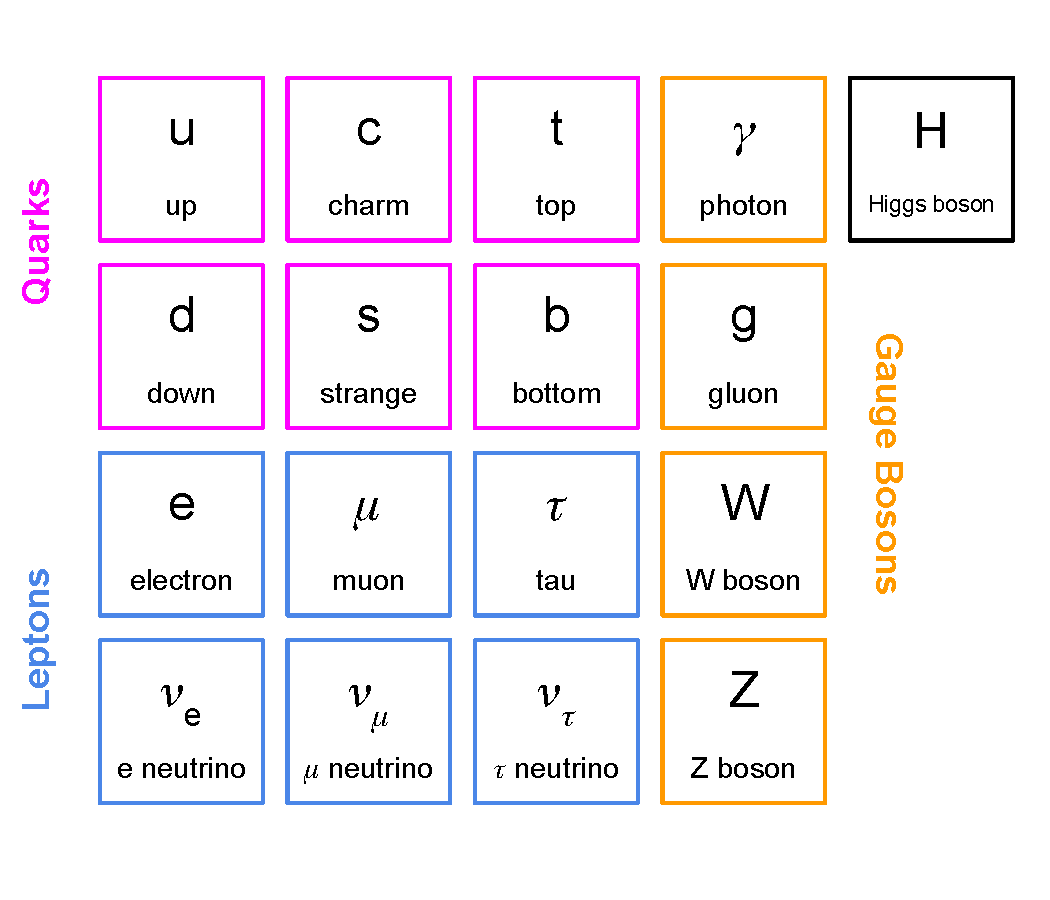
\includegraphics[width=5in]{figures/smparticles.pdf}
\caption{Particles of the Standard Model.}
\label{fig:smparticles}
\end{figure}

The particles of the standard model consist of the spin-$\frac{1}{2}$ fermions, which interact to form regular matter, the spin-1 bosons, which mediate the interactions of the fermions, and the spin-0 scalar Higgs boson, which generates the masses of the bosons and fermions via the Higgs mechanism \cite{Bettini}.

\indent The fermions come in three sets of increasing masses, called generations, corresponding to the first three columns of Figure~\ref{fig:smparticles}. Across the rows, the particles have similar properties and are abbreviated $u^i, d^i, e^i, \nu_e^i$ from top to bottom, where the generation index $i=1,2,3$. Within each generation, the fermions are divided into two categories: (1) the quarks, which are charged under the EM, weak, and strong forces, and (2) the leptons, which are charged under the EM and weak forces. Each fermion has a corresponding antiparticle, whose mass is the same, but whose charges are opposite in sign. The quarks are SU(3) triplets, having a color charge of either R, G, or B. Since the weak force violates $P$, the fermions can be distinguished by their chirality, labeled as either right-handed ($e^i_R$) or left-handed ($e^i_L$). The $(u^i, d^i)_L$ and $(e^i, \nu_e^i)_L$ pairs and their right handed antiparticle pairs are SU(2) doublets and interact via the weak force. The right-handed fermions (left-handed antifermions) are SU(2) singlets and do not interact via the weak force. The weak isospins ($T_3$) for the left handed fermions are: $(u^i, d^i)_L = (\frac{1}{2}, -\frac{1}{2})$ and $(e^i, \nu_e^i)_L = (-\frac{1}{2}, \frac{1}{2})$. The EM charges are $(u^i, d^i)_L = (\frac{2}{3}e, -\frac{1}{3}e)$ and $(e^i, \nu_e^i)_L = (-1e, 0)$, and finally, the weak hypercharges are, $(u^i, d^i)_L = (\frac{1}{3}, \frac{1}{3})$ and $(e^i, \nu_e^i)_L = (-1, -1)$, from the relation $Y_W = 2(Q-T_3)$.

\indent The fourth column of Figure~\ref{fig:smparticles} lists the force mediators, or gauge bosons. The 8 gluons ($g$) of QCD that mediate the strong nuclear force are octets under SU(3) and correspond to linear combinations of the generator gauge fields, $G^a_\mu$. Gluons carry color charge themselves but are electrically neutral. They are massless, consistent with the fact that they correspond to generators of a conserved symmetry, and may be represented using the Gell-Mann matrices as the linearly independent set of states \cite{Griffithsqm}:

\begin{equation}
\begin{split}
\frac{1}{\sqrt{2}}(r\bar{b} + b\bar{r}) \\
\frac{1}{\sqrt{2}}(r\bar{g} + g\bar{r}) \\
\frac{1}{\sqrt{2}}(b\bar{g} + g\bar{b}) \\
\frac{1}{\sqrt{2}}(r\bar{r} - b\bar{b}) \\
-i \frac{1}{\sqrt{2}}(r\bar{b} - b\bar{r}) \\
-i \frac{1}{\sqrt{2}}(r\bar{g} - g\bar{r}) \\
-i \frac{1}{\sqrt{2}}(b\bar{g} - g\bar{b}) \\
\frac{1}{\sqrt{6}}(r\bar{r} + b\bar{b} -2g\bar{g}),
\end{split}
\end{equation}

while the color singlet state that the colorless hadrons are in is:

\begin{equation}
\frac{1}{\sqrt{3}}(r\bar{r} + g\bar{g} + b\bar{b}).
\end{equation}

\indent The remaining gauge bosons, $\gamma$, $W$, and $Z$, mediate the electroweak force. Before electroweak symmetry breaking, the generators of SU(2)$\times$U(1) correspond to the gauge fields \\
$B,\  W^1,\  W^2,\  W^3$, whose excitations are massless gauge bosons. After symmetry breaking via the Higgs mechanism, three of the bosons acquire mass, and the electroweak gauge bosons are reparametrized as:

\begin{equation}
\begin{split}
W^\pm = \frac{1}{\sqrt{2}}(W^1 \pm iW^2) \\
Z = \cos\theta_w W^3 - \sin\theta_w B \\
\gamma = \sin\theta_w W^3 + \cos\theta_w B \\
\end{split}
\end{equation}
where $\theta_w$ is the weak mixing angle, the massive $W^\pm$ and $Z$ bosons mediate the weak force, and the massless $\gamma$ is the photon that mediates EM. the $W^\pm$ bosons have an electric charge of $\pm 1e$, while the $Z$ boson and $\gamma$ are neutral. The isospin of $W^\pm$ are $\pm1$ and 0 for $Z$ and $\gamma$, giving hypercharges of $0$ for $W^\pm$ and 0 for $Z$ and $\gamma$. 

\indent The final particle of the SM is the scalar $H$. $H$ is electrically neutral and constructed to be an SU(2) doublet before electroweak symmetry breaking, with one component having weak isospin $\frac{1}{2}$ (hypercharge $-1$), and the neutral component having isospin $-\frac{1}{2}$ (hypercharge 1), which includes the physical $h$. After electroweak symmetry breaking, three of the $H$ components are absorbed by the gauge bosons, and the remaining physical $h$ remains neutral. The parity of $h$ is 1. Although $H$ couples to all massive fermions and bosons, the decay channels that are relevant for collider searches are: $ZZ^* \rightarrow 4l,\  WW^* \rightarrow 2l2\nu,\  \gamma\gamma,\  \tau\bar{\tau},$ and $b\bar{b}$. After a decades long search, the discovery and verification of quantum numbers of $H$ was announced in 2012 \cite{Chatrchyan:2012xdj, Aad:2012tfa}. The four-lepton invariant mass distribution, showing the $H$ peak at its observed mass of $m_H = 125$ $\GeV$, is shown in Figure~\ref{4l} \cite{CMS:HZZ}.

\begin{figure}[tbh]
\centering
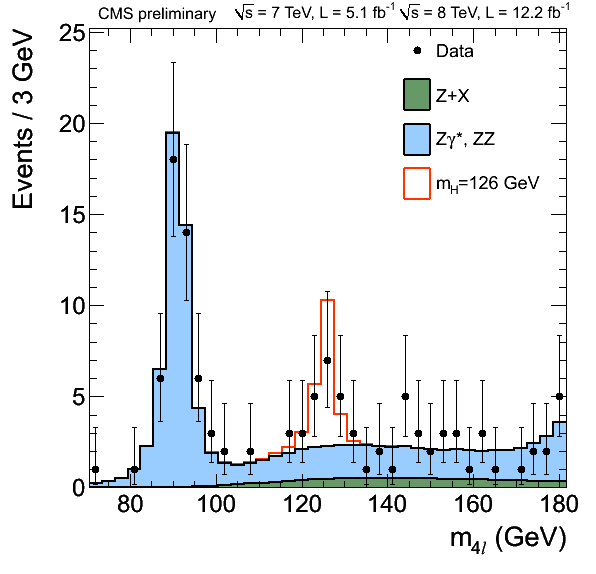
\includegraphics[width=3in]{figures/ZZMass_7Plus8TeV_70-180_3GeV.png}
\caption{Four-lepton invariant mass distribution showing $H$ discovery in the $ZZ^*$ decay channel. The red line shows the signal distribution for $m_H=125$ $\GeV$.}
\label{4l}
\end{figure}


\section{Dark matter}

\subsection{Background}

This section gives an overview of the most compelling sources of observational evidence for the existence of dark matter (DM), the potential particles candidates for DM, and the potential methods for detecting them.  

\subsubsection{Observational evidence}

The earliest indication that there may be matter in the universe that cannot be detected by conventional optical observations, so called dark matter (DM), came from measurements of the orbital velocities of astronomical bodies in galaxy clusters \cite{Kapteyn:1922zz, Zwicky:1937zza} and galaxies \cite{Rubin:1970zza, Rubin:1980zd}. Classical Newtonian gravity gives a galactic rotation curve, which shows how the velocity $v$ of a massive object depends on its distance $r$ from the center of a galaxy, as $v(r) \propto \sqrt{M(r)/r}$, where $M(r)$ is the total mass in the galaxy within a radius $r$. However, measurements of the orbital velocities of objects outside of the visible part of galaxies, where $v(r) \propto 1/\sqrt{r}$, show instead $v(r) \propto$ constant, i.e. that the mass $M(r) \propto r$ instead of being constant \cite{Agashe:2014kda}. The larger than expected velocities imply the existence of this spherically symmetric, dark halo of non-luminous matter in galaxies. 

\indent A compelling example showing direct evidence for DM is galaxy cluster 1E0657-558, often referred to as the "bullet cluster" from its bullet-like shape \cite{Clowe:2003tk}. The bullet cluster passed through another galaxy cluster at some point in the recent cosmological past. The luminous matter, observed by traditional optical telescopes, is seen to lag behind the total mass of the clusters, observed by studying the weak gravitational lensing of objects in the background of the two clusters. The luminous matter in each cluster lags due to its EM interaction with the luminous matter in the opposing cluster, while what is inferred to be the DM continues on a ballistic trajectory, not experiencing lag from EM interactions \cite{Agashe:2014kda}. 

Many other cosmological observations and theories, including observations from strong gravitational lensing in elliptical galaxies \cite{Koopmans:2002qh}, observations from weak lensing of distant galaxies by foreground matter \cite{Hoekstra:2002nf}, and modeling of anisotropies in the cosmic microwave background (CMB) \cite{Hu:2001bc, Hu:1996qs}, strongly support the existence of DM, and other than a handful of competing theories which modify the laws of gravity instead of adding new matter, the existence of DM is widely accepted \cite{Bertone:2004pz} and is believed to account for $20-40$\% of the mass density of the universe \cite{Bergstrom:2000pn}.

\subsubsection{Particle candidates}

From a variety of searches for different types of new dark particles, much more is known about what DM is not than what it is. Surveys are made to detect gravitational microlensing from massive compact halo objects (MACHOs), such as black holes, dwarf stars, and neutron stars, that could be baryonic matter faking DM. These objects cannot account for the majority of DM \cite{Tisserand:2006zx, Wyrzykowski:2011tr}. In fact, Big Bang nucleosynthesis, the theory of how light nuclei were produced in the early universe, shows that measurements of the abundances of elements today suggest that most of DM is non-baryonic \cite{Copi:1994ev}. Measurements of CMB anisotropies determine the density of non-baryonic matter, an important constraint on potential DM candidates \cite{Agashe:2014kda}. For example, the only SM particles that could potentially account for DM are neutrinos, but these are excluded because they are not abundant enough to account for the DM density \cite{Bertone:2004pz}. 

\indent For all that is unknown about the particle content of the dark sector, there are several properties of DM that are known with high confidence: (1) it does not interact via the EM force, or this interaction is highly suppressed, (2) it is stable over long time scales, (3) it has a relic density consistent with cosmological observations, and (4) it is "cold", meaning it was non-relativistic by the time galaxies were beginning to form \cite{Bertone:2004pz}. A plethora of candidates satisfying these properties has been developed, including sterile neutrinos, like SM neutrinos but that do not interact via the weak force \cite{Dodelson:1993je}, axions, theoretical particles developed to address CP violation \cite{Rosenberg:2000wb}, and particles from "little Higgs" models \cite{BirkedalHansen:2003mpa, Cheng:2003ju}, just to name a few. 

\indent The most widely studied candidates, however, are weakly interacting massive particles (WIMPs), with masses in the range of 10 $\GeV$ to a few $\TeV$, and whose self-annihilation cross section is similar in scale to the weak strength \cite{Bertone:2004pz}. The two best motivated WIMPs are the lightest superparticle (LSP) of supersymmetric (SUSY) models \cite{Jungman:1995df} and the lightest Kaluza-Klein particle (LKP) of models with extra dimensions \cite{Kolb:1983fm}. The SUSY model should obey R-parity to guarantee the stability of the LSP. The LSP should be neutral to satisfy constraints from searches for exotic isotopes and is unlikely to be an ordinary sneutrino, which would have been observed in previous WIMP searches \cite{Agashe:2014kda}. This leaves the lightest neutralino, a mixture of the gauge boson superpartner gauginos, as the best DM candidate from SUSY models. Alternatively, models introducing extra spatial dimensions, such as those of Arkani-Hamed, Dimopoulos, and Dvali (ADD) \cite{ArkaniHamed:1998rs} and Randall and Sundrum (RS)\cite{Randall:1999ee}, predict a "tower" of excited states of SM particles, called Kaluza-Klein (KK) states, with increasing mass proportional to the inverse of the scale of the extra dimension, and having the same quantum numbers as their corresponding SM particles. Models where all SM fields can propagate in the extra dimensions, as opposed to models where only gravity can, are called universal extra dimensions (UED) \cite{Appelquist:2000nn}. The best motivated LKP is the first KK excitation in UED of the SM U(1) gauge boson \cite{Cheng:2002iz}. 

\subsubsection{Potential detection methods}

The methods of detecting DM fall into three categories: (1) indirect searches, where the products of DM annihilations or decays are observed, (2) direct searches, where the recoil of SM particles is measured after scattering with an incident DM particle, and (3) collider searches, where the DM candidate is produced directly from interactions of SM particles. These methods complement one another since they each approach the problem in a different way and have different relative strengths and weaknesses. For example, direct searches are limited in their sensitivities at low DM masses by the inability to measure such smaller nuclear recoils, while colliders excel in this region since the production of low mass particles is uninhibited by kinematic restrictions. Conversely, collider searches are less sensitive than direct and indirect searches at high mass, being limited by the energy scale of the collisions.

\indent Indirect DM searches are performed at experiments designed to detect the SM products of the decays or self-annihilations of DM particles. Since DM is attracted by the gravitational force, it could collect in the centers of massive bodies such as the Sun or Earth, where they would be more likely to annihlate in higher densities. The IceCube detector sets the best upper limits on the high-energy muon flux from DM annihilations within the Sun to 103 muons/$\rm{km}^2$/yr \cite{PhysRevLett.110.131302}, while the SuperKamiokande telescope has the best upper limits for softer muons at about 1500 muons/$\rm{km}^2$/yr \cite{0004-637X-742-2-78}. Searches for photons from DM annihilating in the galactic halo can produce monoenergetic photon spectra, but these signals are particularly difficult to isolate from photons of regular astrophysical origin. The FERMI/LAT collaboration has found a small signal in a region around the galactic center, with known point sources removed from the data, but the result is not strong enough to be considered a discovery \cite{Ackermann:2013uma}. Finally, DM can produce an excess in the spectra of antiparticles such as positrons. Experiments find small excesses with these signatures, but they may be explained by astrophysical sources, and they predict a DM cross section too high to be consistent with a thermal WIMP \cite{Agashe:2014kda}.

\indent Direct DM searches measure the interaction of DM with regular matter through either elastic or inelastic collisions, in either a spin-dependent or spin-independent manner in terrestrial laboratory detectors \cite{Bertone:2004pz}. In an elastic scattering experiment, WIMPs interact with the nuclei in the detector as a whole, and the recoil energy spectrum is measured, typically in the range 1-100 $\keV$. In inelastic scattering experiments, the WIMP either excites or ionizes orbital electrons, or the WIMP leaves the nuclei in the detector in an excited state, yielding an energy recoil of the nucleus plus an emitted photon a short time later. These target interactions are also distinguished by whether the DM-nucleon interactions involve the spin degree of freedom of the nuclei. Spin-independent detectors benefit from an increase in the DM-nucleon interaction cross section by increasing the mass of the detector nuclei, while the mass of the detector material does not benefit the spin-dependent measurements to the same degree. The best cross section lower limits for spin-indenpendent and spin-dependent neutron interactions come from the Large Underground Xenon (LUX) detector, a time-projection chamber filled with 368 kg of scintillating liquid xenon, surrounded by highly sensitive light detectors to search for the signature of DM scattering with a xenon atom, and shielded by a large water tank and a mile of Earth overburden \cite{Akerib:2016lao}. For a WIMP mass of 33 $\GeV$, the cross section lower limits from LUX are on the order of $10^{-45} \rm{cm}^2$ for spin-independent, and $10^{-41}(10^{-39}) \rm{cm}^2$ for spin-independent neutron(proton) interactions.

\indent Finally, DM can be produced directly in particle colliders, and searches for signatures of high missing energy from DM escaping the detector opposite a tagged SM particle can be explored. Such signatures are referred to as mono-$X$, where $X$ is the single SM particles observed in the detector. Note that since the DM is produced and is not from cosmic origins, collider searches are not traditional DM searches, where the target signal originates from the cosmic dark matter. Consequently, a DM-like particle produced and detected at a collider experiment, displaying some of the expected properties, may mimic cosmic DM, but may not be stable on cosmological time scales \cite{Askew:2014kqa}. The methods of collider searches are covered in detail in the next section, including the current statuses of these searches. 

\indent When the observations of either of the three detection methods are consistent with the backgrounds only and no signal is observed, the results are cast in the form of exclusion limits, and special care must be taken to compare these limits between the different methods. Of particular interest is the comparison of DM cross section upper limits between direct and collider searches. In order to compare the DM-nucleon cross sections from direct and indirect searches to the mono-$X$ production cross sections from collider searches, a model for how DM couples to nucleons must be specified. For comparisons to the spin-independent cross section upper limits for DM scattering off a nucleus $N$ found by LUX, the following relation will be used:

\begin{equation}
\sigma^{SI}_{\chi N} = \frac{\mu^2_{\chi N}}{\pi} [Zf_p + (A-Z)f_n]^2
\end{equation}
where $\mu_{\chi N} = $ is the $\chi-N$ reduced mass, $A$ and $Z$ are the atomic mass numbers of $N$, and $f_{p/n}$ are the model-dependent couplings of DM to protons/neutrons \cite{Carpenter:2013xra}. A set of models describing the explicit coupling of DM to SM particles is detailed in the next section.

\section{Beyond the Standard Model}

\subsection{Collider searches for DM}

Previous DM searches at the Large Hadron Collider (LHC) include analyses with mono-$X$ signatures: $X$ produced in association with large missing transverse momentum (MET) from the DM escaping the detector, where $X$ is a jet \cite{Aad:2015zva, Khachatryan:2014rra}, $t$/$b$ quark \cite{Aad:2014vea, Khachatryan:2014uma, Khachatryan:2015nua}, photon \cite{Aad:2014tda, Chatrchyan:2012tea, Khachatryan:2014rwa}, lepton \cite{Khachatryan:2014tva, ATLAS:2014wra}, or $W$/$Z$ boson \cite{Aad:2014vka, Aad:2013oja, Khachatryan:2015bbl}. The discovery of the Higgs boson has opened a new portal to searching for DM at the LHC through the mono-$H$ signature \cite{Carpenter:2013xra, Berlin:2014cfa}. 

\indent Mono-$H$ is purely a discovery mode for DM. Due to the distinct production topologies and suppressed couplings, mono-$H$ analyses cannot contribute to the combination of other mono-$X$ analyses. In contrast with other mono-$X$ signatures, in which $X$ is emitted as initial state radiation (ISR)(see Figure~\ref{fig:isr}), ISR of a $H$ is highly suppressed due to the small $H$-quark coupling. Therefore, the $H$ is radiated preferentially from the new physics vertex (see Figure~\ref{fig:fsr}), directly probing the effective DM-SM coupling. The models describing the effective vertex for the case where $X$ comes from ISR, referred to as ISR models, couple DM to quarks either through effective field theory (EFT) operators, or explicitly with a scalar or vector mediator \cite{Abercrombie:2015wmb}. Since the effective vertex does not explicitly involve $X$, the different mono-$X$ searches can be combined, each carrying a weight proportional to the quark-$X$ coupling. Since the quark-$H$ coupling is small compared to the other quark-$X$ couplings, mono-$H$ cannot make a strong contribution to the combination, and is therefore not included. The models that have $X$ emitted directly from the effective vertex, referred to as discovery models, do have a well-motivated mono-$H$ signature. These models couple DM to $X$ directly with EFT operators or a new mediator particle, so not all mono-$X$ analyses are combined as in the ISR case. Each mono-$X$ signature has discovery models that motivate an enhanced DM-$X$ coupling, so although some signatures can be combined for these models, with comparable contributions, they are usually studied independently for the different signatures. These models are called discovery models because they each allow for the detection of DM for each mono-$X$ signature, independently from the others. Therefore, even though the signatures contribute different amounts to the ISR model combinations, it is of critical importance to look at each signature's discovery models. This dissertation will consist of the study of the discovery models for mono-$H$. 

\begin{figure}[tbh]
\centering
\begin{subfigure}{0.45\textwidth}
\centering
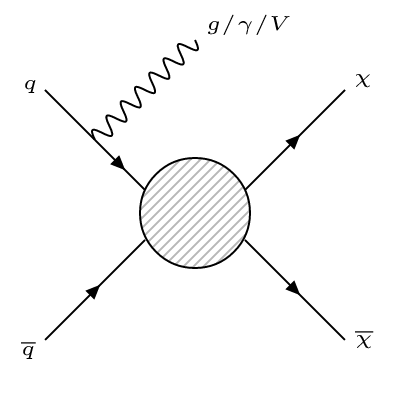
\includegraphics[width=2in]{figures/isr.png}
\caption{}
\label{fig:isr}
\end{subfigure}
\begin{subfigure}{0.45\textwidth}
\centering
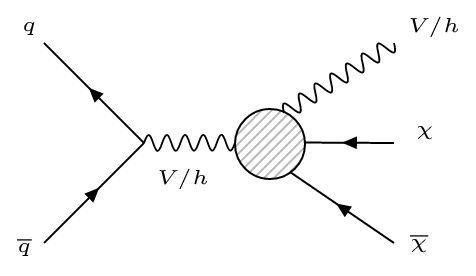
\includegraphics[width=2.5in]{figures/fsr.png}
\caption{}
\label{fig:fsr}
\end{subfigure}
\caption{(a) Mono-$X$ production topology for signatures with $X$ emitted as ISR. (b) Mono-$X$ production topology for signatures with $X$ emitted from new physics vertex.}
\label{monox}
\end{figure}

Mono-$H$ searches have been done at the 8 $\TeV$ LHC for H decaying to two photons \cite{Aad:2015yga} and two bottom quarks \cite{Aad:2015dva} at ATLAS, with results consistent with SM predictions and limits set on various model parameters. The $b\bar{b}$ final state shows a higher sensitivity to limit setting for the models used in the data interpretation at 8 $\TeV$. For 13 $\TeV$ LHC data, mono-$H$ searches are being done at ATLAS for $H$ to $b\bar{b}$ \cite{Atlas:2016Hbb} and at CMS for the five H decay modes: $ZZ$, $WW$ \cite{CMS-AN-15-338}, $\gamma\gamma$ \cite{CMS-AN-15-203}, $b\bar{b}$ \cite{CMS-AN-15-209}, and $\tau\tau$. Because each final state will have various benefits and drawbacks, each has a dedicated analysis, exploring the sensitivity to different models in different regions of parameter space.

The $H\rightarrow ZZ$ decay mode, where the two $Z$ bosons decay to four leptons, is studied in this dissertation. The mode where the $Z$ bosons decay to two leptons and two neutrinos is open for investigation. Over other $H$ decay modes, the four-lepton final state has the advantage of easily reducible backgrounds and a clean reconstruction of final state particles. The lepton combinations of four electrons, four muons, and two electrons two muons are treated individually, then combined in the final results. This channel was key to the discovery of $H$ at 7 and 8 $\TeV$ \cite{Chatrchyan:2013mxa, ATLAS:2013nma}, and this analysis is an extension of these studies and their continuation \cite{CMS-AN-15-277, CMS-PAS-HIG-15-004}. In particular, the baseline event selection used here is chosen to match that of the other $H\rightarrow ZZ$ analysis groups through an event by event synchronization exercise \cite{synchtwiki}.

Nine kinematically distinct models with DM are used in the data interpretation, including five effective field theory (EFT) models and four simplified models. The EFT models couple DM to $H$ via an $n$-dimensional contact operator, with operators of dimension four, five, six, and eight \cite{Carpenter:2013xra}. They have the benefit of being independent of the details of new physics models and having a one-dimensional parameter space. The EFTs have the drawback of limited ranges of validity, being constrained by perturbativity and $H$ and $Z$ to invisible decay limits. The EFT parameter choices are discussed in the next section. The simplified models introduce an additional massive particle to mediate the DM-SM coupling. This mediator particle is a vector, scalar, or pseudoscalar \cite{Carpenter:2013xra, Berlin:2014cfa}. Although they are better motivated by the addition of new physics, the simplified models have the drawback of more complex parameter spaces, including parameters which affect the kinematics of the final state particles and must be scanned over. The simplified model parameter choices discussed in Section~\ref{sec:sigmodels} are chosen to be consistent with other LHC DM searches \cite{Abercrombie:2015wmb}.

\subsection{Signal models}
\label{sec:sigmodels}
The signal models are divided into two categories: effective field theories (EFTs) and simplified models.

\subsubsection{Effective field theory models and benchmarks}

The five EFTs are summarized in Table~\ref{tab:efts}. The models have Lagrangians with effective operators ranging from dimension four to eight with either scalar or fermionic DM \cite{McDonald:1993ex, LopezHonorez:2012kv}, producing mono-$H$ signatures shown in Figure~\ref{fig:eftsig}. The models have two parameters each, the DM mass and the coupling or mass cutoff scale. Although there are regions of parameter space where the kinematics are independent of the coupling or mass cutoff scale, the kinematics generally depend on the choice of both parameters. The DM mass values are the same for all models: 1, 10, 50, 65, 100, 200, 400, 800, 1000, 1300 $\GeV$, as recommended by the LHC DM Working Group (DMWG) \cite{Abercrombie:2015wmb}. These mass values are chosen with a fine enough grid spacing to cover the range of variation in kinematics. The additional value of 65 $\GeV$, around half the Higgs' mass, is added where the cross sections begin to drop significantly and assists in producing smooth limit curves.

\begin{figure}[tbh]
\centering
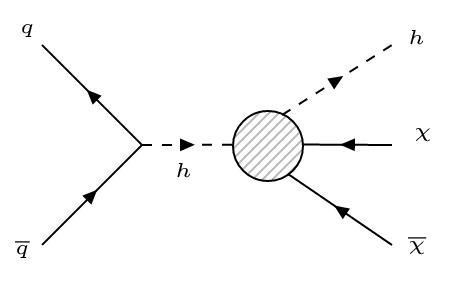
\includegraphics[width=3in]{figures/eftsig.png}
\caption{Collider production diagram for mono-Higgs effective field theories.}
\label{fig:eftsig}
\end{figure}

The value of the coupling must be set for each model individually so as to ensure the value is in a range where the kinematics are independent of the coupling. In these regions of parameter space, cross section limits can be reliably scaled to coupling limits. The additional value of $\Lambda = 1000 \GeV$ for EFT$\_$xdxHDHc is included to compare with previous limits, even though it is in the region where the kinematics depend on the coupling. Existing constraints on the couplings from perturbativity \cite{Carpenter:2013xra} and invisible branching ratio limits \cite{Belanger:2013kya, PhysRevD.86.010001} are shown in Table~\ref{tab:eftlims}. The constraints from invisible branching ratio limits only apply when the DM mass is less than half the mediator mass, allowing this decay to be kinematically open. The production cross sections for these benchmark choices are given in Appendix A.

\begin{table*}[htbH]
\begin{center}
\begin{tabular}{ l | c | l | c | c}
\hline
Name & Operator & Param. & Dim. & $S_{\chi}$ \\
\hline
EFT$\_$HHxx$\_$scalar & $\lambda |H|^{2} \chi^{2}$ & $m_{\chi}, \lambda = 0.1$ & 4 & 0 \\
EFT$\_$HHxx$\_$combined & $\frac{1}{\Lambda} |H|^{2} \bar{\chi} \chi$ & $m_{\chi}, \Lambda = 1000$ $\GeV$ & 5 & 1/2 \\
EFT$\_$HHxxg5x & $\frac{1}{\Lambda} |H|^{2} \bar{\chi} i \gamma_{5} \chi$ & $m_{\chi}, \Lambda = 100$ $\GeV$ & 5 & 1/2\\
EFT$\_$xdxHDHc & $\frac{1}{\Lambda^{2}} \chi^{\dag} i \partial^{\mu} \chi H^{\dag} i D_{\mu} H $ & $m_{\chi}, \Lambda = 100,1000$ $\GeV$ & 6 & 0\\
EFT$\_$xgxFHDH & $\frac{1}{\Lambda^{4}} \bar{\chi} \gamma^{\mu} \chi B_{\mu\nu} H^{\dag} D^{\nu} H$ & $m_{\chi}, \Lambda = 200$ $\GeV$ & 8 & 1/2\\
\hline
\end{tabular}
\caption{Effective Field Theory Models \cite{Carpenter:2013xra}.}\label{tab:efts}
\end{center}
\end{table*}

\begin{table*}[htbH]
\begin{center}
\begin{tabular}{ l | c | l}
\hline
Name & Perturbativity & $BR_{inv}$ Limits \\
\hline
EFT$\_$HHxx$\_$scalar & $\lambda < 4\pi$ & $\lambda < 0.016$ ($m_\chi < m_h/2$)\\
EFT$\_$HHxx$\_$combined & $\Lambda > v/4\pi $ & $\Lambda > 10$ $\TeV$ ($m_\chi < m_h/2$)\\
EFT$\_$HHxxg5x & $\Lambda > v/4\pi $ & $\Lambda > 10$ $\TeV$ ($m_\chi < m_h/2$) \\
EFT$\_$xdxHDHc & $g_Z < 4\pi$, $\Lambda > 30$ $\GeV$ & $\Lambda > 400$ $\GeV$ ($m_\chi < m_Z/2$) \\
\hline
\end{tabular}
\caption{Constraints on effective field theory model parameters \cite{Carpenter:2013xra}.}\label{tab:eftlims}
\end{center}
\end{table*}

\subsubsection{Simplified models}

\indent There are four simplified models, each including one or more new massive particles that mediate the $H$-DM interaction. The models with vector mediators are motivated by the addition of new symmetries to the Standard Model, with the mediator corresponding to the gauge boson of the new symmetry. Additional models are motivated by the addition of scalar or pseudoscalar mediators as a portal into the dark sector.

\subsubsection{$Z'$ - Two Higgs doublet model}

The $Z'$ - Two Higgs Doublet Model (Zp2HDM) simplified model extends the gauge group of the SM to include a new symmetry, $U(1)_{Z'}$, with $Z'$ the gauge boson \cite{Berlin:2014cfa}. This symmetry is spontaneously broken by a scalar singlet $\phi$, generating a $Z'$ mass above the electroweak (EW) symmetry breaking scale. The right-handed quarks are charged under $U(1)_{Z'}$ and all other SM particles are neutral. The $Z'$ coupling to quarks, $g_z$, is constrained by EW global fits \cite{PhysRevD.86.010001} and dijet resonance searches \cite{Aaltonen:2008dn, Chatrchyan:2013qha} to be:

\begin{equation}
g_z < 0.03 \frac{g}{\cos\theta_w\sin^2\beta}\frac{\sqrt{M_{Z'}^2-M_Z^2}}{M_Z}.
\end{equation}

Additionally, a second Higgs doublet is added with a Type 2 two-Higgs doublet model, introducing states $\Phi_u$ and $\Phi_d$, which couple to up and down type quarks, respectively, as:

\begin{equation}
\mathcal{L} \supset -y_u Q \bar{\Phi}_u \bar{u} - y_d Q \Phi_d \bar{d} + y_e L \Phi_d \bar{e} + h.c..
\end{equation}

$\Phi_u$ is chosen to be charged under $U(1)_{Z'}$, while $\Phi_d$ is neutral. The two Higgs doublets obtain VEVs $\nu_u$ and $\nu_d$ after EW symmetry breaking and can be parametrized as:

\begin{equation}
\begin{split}
\Phi_d = \frac{1}{\sqrt{2}} \begin{pmatrix}-\sin(\beta) H^{+} \\ \nu_d - \sin(\alpha)h + \cos(\alpha)H - i\sin(\beta)A^0 \end{pmatrix} \\
\Phi_u = \frac{1}{\sqrt{2}} \begin{pmatrix} \cos(\beta)H^{+} \\  \nu_u + \cos(\alpha)h + \sin(\alpha)H + i\cos(\beta)A^0 \end{pmatrix}
\end{split}
\end{equation}
where $h$ and $H$ are neutral $CP$-even scalars, and $A^0$ is $CP$-odd. The angle $\alpha$ is defined as the angle that diagonalizes the $h-H$ mass mixing matrix, and the angle $\beta$ is defined as $\tan(\beta) = \nu_u / \nu_d$. The $h$ is assumed to be the SM Higgs boson with $m_h = 125$ $\GeV$, while the other scalars have masses $> 300$ $\GeV$. Due to perturbativity and previous constraints \cite{Craig:2013hca}, $\alpha$ and $\beta$ are chosen such that $\tan(\beta)>0.3$ and $\alpha = \beta - \pi/2$.

Mono-$H$ signals arise when the pseudoscalar $A^0$ has a large branching ratio to DM, as shown in Figure~\ref{fig:zp2hdmsig}. The new particles and parameters of the Zp2HDM model are summarized in Table~\ref{tab:Zp2HDM}. The values of the parameters chosen for various benchmark scenarios are given Section~\ref{sec:sigbench}.

\begin{figure}[tbh]
\centering
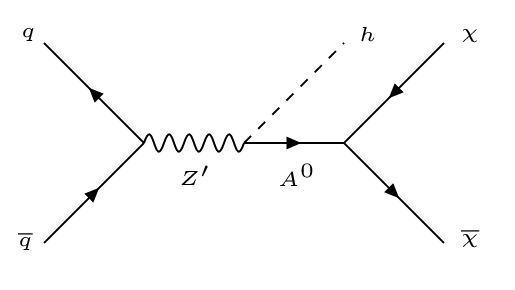
\includegraphics[width=3in]{figures/zp2hdmsig.png}
\caption{Collider production diagram for Zp2HDM.}
\label{fig:zp2hdmsig}
\end{figure}

\begin{table*}[htbH]
\begin{center}
\begin{tabular}{ l | l}
\hline
Particle & Description \\
\hline
$\chi$ & Fermionic DM particle \\
Z' & $U(1)_{Z'}$ gauge boson \\
$\phi$ & Z' sector scalar \\
$\Phi_u, \Phi_d$ & Two Higgs doublets \\
$h, H$ & Neutral CP-even scalars \\
$H^\pm$ & Charged heavy Higgs \\
$A^0$ & Neutral CP-odd pseudoscalar \\
\hline
Param. & Description \\
\hline
$m_\chi$ & DM mass \\
$m_{Z'}$ & Z' mass \\
$g_z$ & Z'-quark coupling \\
$y_{u/d/e}$ & $\Phi$-up-quark/down-quark/lepton coupling \\
$\nu_{u/d}$ & $\Phi_{u/d}$ VEV \\
$\alpha$ & $h$-$H$ mixing angle \\
$\beta$ & $\Phi_{u/d}$ VEV angle \\
\hline
\end{tabular}
\caption{New particles and parameters of the Zp2HDM simplified model \cite{Carpenter:2013xra}}\label{tab:Zp2HDM}
\end{center}
\end{table*}


\subsubsection{Baryonic $Z'$ model}

The Baryonic $Z'$ (ZpBaryonic) simplified model extends the gauge group of the SM to include a new symmetry, $U(1)_B$ for the baryon number $B$, with the $Z'$ being the gauge boson of $U(1)_B$ \cite{Carone:1994aa, Agashe:2004bm, FileviezPerez:2010gw}. $Z'$ couples to quarks and fermionic DM as:

\begin{equation}
\mathcal{L} \supset g_q \bar{q} \gamma^\mu q Z'_\mu + g_\chi \bar{\chi} \gamma^\mu \chi Z'_\mu
\end{equation}

To derive a mono-Higgs signature, $U(1)_B$ is spontaneously broken by a "baryonic Higgs" scalar $h_B$, which mixes with the SM Higgs via a mixing angle $\theta$. This mixing induces an $h-Z'$ interaction $-g_{hZ'Z'} h Z'_\mu Z'^\mu$, with coupling:

\begin{equation}
g_{hZ'Z'} = \frac{m_{Z'}^2 \sin(\theta)}{\nu_B}
\end{equation}
where $m_{Z'}$ is the mass of the $Z'$ and $\nu_B$ is the VEV of $h_B$. At energies less than $m_{Z'}$, these operators combine to yield an effective Lagrangian:

\begin{equation}
\mathcal{L}_{eff} = -\frac{g_q g_\chi}{m_{Z'}^2} \bar{q} \gamma^\mu q \bar{\chi} \gamma_\mu \chi (1 + \frac{g_{hZ'Z'}}{m_{Z'}^2} h)
\end{equation}
The first term gives rise to mono-jet and mono-EW boson signals, while the second yields the mono-Higgs signal shown in Figure~\ref{fig:zpsig}.

\begin{figure}[tbh]
\centering
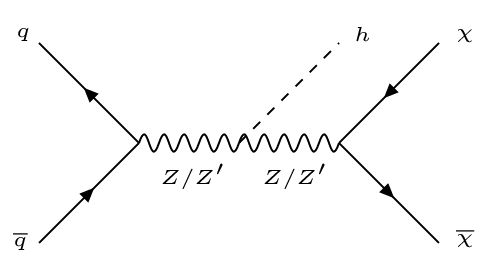
\includegraphics[width=3in]{figures/zpsig.png}
\caption{Collider production diagram for Z' models.}
\label{fig:zpsig}
\end{figure}

The new particles and parameters of the ZpBaryonic model are summarized in Table~\ref{tab:ZpBaryonic}. Perturbativity arguments require the $Z'$-quark coupling to be less than $4\pi$ \cite{Carpenter:2013xra}. The values of the parameters chosen for various benchmark scenarios are given in Section~\ref{sec:sigbench}.

\begin{table*}[htbH]
\begin{center}
\begin{tabular}{ l | l}
\hline
Particle & Description \\
\hline
$\chi$ & Fermionic DM particle \\
Z' & $U(1)_B$ gauge boson \\
$h_B$ & Baryonic Higgs \\
\hline
Param. & Description \\
\hline
$m_\chi$ & DM mass \\
$m_{Z'}$ & Z' mass \\
$g_q$ & Z'-quark coupling \\
$g_\chi$ & Z'-DM coupling \\
$g_{hZ'Z'}$ & Z'-h coupling \\
$\theta$ & $h$-$h_B$ mixing angle \\
$\nu_B$ & $h_B$ VEV \\
\hline
\end{tabular}
\caption{New particles and parameters of the ZpBaryonic simplified model \cite{Carpenter:2013xra}}\label{tab:ZpBaryonic}
\end{center}
\end{table*}

\subsubsection{Hidden sector $Z'$ model}

The Hidden Sector $Z'$ (ZpHS) simplified model mixes the SM and a hidden sector with a $U(1)'$ symmetry \cite{Chang:2006fp, Pospelov:2007mp, Feldman:2007wj, Feng:2008mu, Gopalakrishna:2008dv}. SM particles are neutral under $U(1)'$, while DM is charged. The relevant terms in the Lagrangian are:

\begin{equation}
\mathcal{L}_{eff} \supset \frac{g_2}{2c_W} J^\mu_{NC} Z_\mu + g_\chi \bar{\chi} \gamma^\mu \chi Z'_\mu
\end{equation}
where $J_{NC}$ is the SM neutral current. A mono-Higgs signature arises from a $Z-Z'$ mass mixing, which is diagonalized by the rotation:

\begin{equation}
Z \rightarrow \cos(\theta) Z - \sin(\theta) Z', Z' \rightarrow \cos(\theta) Z' + \sin(\theta) Z
\end{equation}

This mixing yields the mono-Higgs signatures shown in Figure~\ref{fig:zpsig} through the $h-Z-Z'$ interaction: 

\begin{equation}
\mathcal{L}_{eff} \supset \frac{m_Z^2 \sin(\theta)}{\nu} h Z'_\mu Z^\mu
\end{equation}

The new particles and parameters of the ZpHS model are summarized in Table~\ref{tab:ZpHS}. In order to be consistent with the invisible $Z$ width of $\Lambda(Z\rightarrow \chi\bar{\chi})<3$ $\MeV$, the value of $\theta$ is constrained by $\sin\theta<0.03$ for $m_\chi < m_z/2$ \cite{PhysRevD.86.010001}. The values of the parameters chosen for various benchmark scenarios are given in Section~\ref{sec:sigbench}.

\begin{table*}[htbH]
\begin{center}
\begin{tabular}{ l | l}
\hline
Particle & Description \\
\hline
$\chi$ & Fermionic DM particle \\
Z' & $U(1)'$ gauge boson \\
\hline
Param. & Description \\
\hline
$m_\chi$ & DM mass \\
$m_{Z'}$ & Z' mass \\
$g_\chi$ & Z'-DM coupling \\
$\theta$ & $Z$-$Z'$ mixing angle \\
\hline
\end{tabular}
\caption{New particles and parameters of the ZpHS simplified model \cite{Carpenter:2013xra}}\label{tab:ZpHS}
\end{center}
\end{table*}

\subsubsection{Scalar mediator model}

The Scalar Mediator (Scalar) simplified model introduces a real scalar singlet S as a portal into the dark sector \cite{MarchRussell:2008yu}. The quark and DM Yukawa coupling terms are:

\begin{equation}
\mathcal{L} \supset -y_\chi \bar{\chi} \chi S - \frac{m_q}{\nu} \bar{q} q h
\end{equation}
and the relevant terms of the scalar potential are:

\begin{equation}
V \supset a |H|^2 + b |H|^2 S^2 + \lambda_h |H|^4 \rightarrow \frac{1}{2} a (h+\nu)^2 S + \frac{1}{2} b (h+\nu)^2 S^2 + \frac{\lambda_h}{4}(h+\nu)^4.
\end{equation}
The expression after the arrow follows when the Higgs acquires a VEV, as $H \rightarrow \frac{1}{\sqrt{2}} (h + \nu)$. After expanding the expression, there is an $h-S$ mixing term $a\nu hS$. The system can be diagonalized with the rotation:

\begin{equation}
h \rightarrow \cos(\theta) h + \sin(\theta) S, S \rightarrow \cos(\theta) S - \sin(\theta) h
\end{equation}
where $\theta$ is defined by $\sin(2\theta) = 2a\nu/(m_S^2-m_h^2)$. Following this rotation, the Yukawa terms become:

\begin{equation}
\mathcal{L} \supset -y_\chi \bar{\chi} \chi (\cos(\theta) S - \sin(\theta) h) - \frac{m_q}{\nu} \bar{q} q (\cos(\theta) h + \sin(\theta) S)
\end{equation}
and the relevant terms in the scalar potential, at first order in $\sin(\theta)$, are:

\begin{equation}
V \supset \frac{\sin(\theta)}{\nu}(2m_h^2 + m_S^2) h^2 S + b \nu h S^2.
\end{equation}
These terms give rise to the mono-Higgs interactions shown in Figure~\ref{fig:scsig}, as well as additional loop diagrams for gluon fusion production. The new particles and parameters of the Scalar model are summarized in Table~\ref{tab:Scalar}. Perturbativity arguments require $\sin\theta<4\pi$ \cite{Carpenter:2013xra}, while 8 $\TeV$ $H$ data is consistent with $\cos\theta=1$, requiring $\sin\theta<0.4$ \cite{Falkowski:2013dza, Djouadi:2013qya, Giardino:2013bma, Ellis:2013lra}. The values of the parameters chosen for various benchmark scenarios are given in Section~\ref{sec:sigbench}.

\begin{figure}[tbh]
\centering
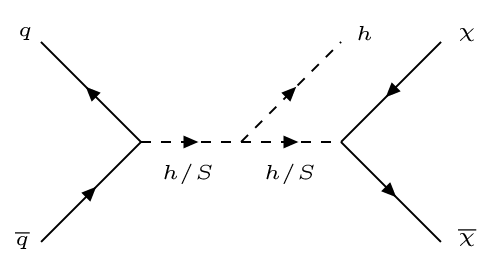
\includegraphics[width=3in]{figures/scsig.png}
\caption{Collider production diagram for Scalar model.}
\label{fig:scsig}
\end{figure}

\begin{table*}[htbH]
\begin{center}
\begin{tabular}{ l | l}
\hline
Particle & Description \\
\hline
$\chi$ & Fermionic DM particle \\
S & Scalar particle \\
\hline
Param. & Description \\
\hline
$m_\chi$ & DM mass \\
$m_{S}$ & S mass \\
$y_\chi$ & S-DM coupling \\
$a, b$ & $h$-$S$ scalar couplings \\
$\theta$ & $h$-$S$ mixing angle \\
\hline
\end{tabular}
\caption{New particles and parameters of the Scalar simplified model \cite{Carpenter:2013xra}}\label{tab:Scalar}
\end{center}
\end{table*}


\subsubsection{Benchmarks}\label{sec:sigbench}

The simplified models are summarized in Table~\ref{tab:sms}. Although these models have better physical motivations, the parameter spaces are vastly more complex than the EFTs, making it difficult to understand the cross section scaling rules and kinematic dependence on parameters accross the entire parameter spaces. The parameter values are chosen to match the recommendations of the DMWG \cite{Abercrombie:2015wmb}. For the ZpHS model, which is not included in the DMWG report, the coupling parameters are chosen to match the benchmarks of Carpenter et al. \cite{Carpenter:2013xra} while the DM and mediator mass scan matches the DMWG recommendations for a vector mediator, shown in Table~\ref{tab:MMVector}. The DM and mediator mass scans for the Zp2HDM and Scalar models are shown in Table~\ref{tab:MM2HDM} and Table~\ref{tab:MMScalar}, respectively. Existing constraints on the couplings from theory and invisible branching ratio limits given in are shown in Table~\ref{tab:smlims} \cite{Carpenter:2013xra}. The production cross sections for the simplified models are given in Appendix A. 

\begin{table*}[htbH]
%\begin{center}
%\begin{adjustbox}{width=\textwidth,totalheight=\textheight,keepaspectratio}
\begin{tabular}{ l | c | c | c}
\hline
Name & Mediator($S_{\rm{Mediator}}$) & Fixed Param. & Scanned Param.\\
\hline
Zp2HDM & Z'(1/2) & $m_\chi = 100$ $\GeV$ & ($m_{Z'}$,$m_{A^0}$) = Table~\ref{tab:MM2HDM} \\
 & $A^0$(0) & $g_Z = 0.8$ &  \\
 & & $\tan\beta = 1$ &  \\
\hline
ZpBaryonic & Z'(1/2) & $g_\chi = 1$ & ($m_{Z'}$,$m_\chi$) = Table~\ref{tab:MMVector} \\
 & & $g_q = 1/3$ &  \\
 & & $g_{hZ'Z'} = m_{Z'}$ &  \\
\hline
ZpHS & Z'(1/2) & $g_\chi = 1$ & ($m_{Z'}$,$m_\chi$) = Table~\ref{tab:MMVector} \\
 & & $\sin(\theta) = 0.1$ & \\
\hline
Scalar & S(0) & $g_\chi = 1$ & ($m_{S}$,$m_\chi$) = Table~\ref{tab:MMScalar}\\
 & & $\sin(\theta) = 0.3$ & \\
 & & $b = 3$ & \\
\hline
\end{tabular}
\caption{Benchmark parameter choices for the simplified models \cite{Carpenter:2013xra, Abercrombie:2015wmb}.}\label{tab:sms}
%\end{adjustbox}
%\end{center}
\end{table*}

\begin{table*}[htbH]
\begin{center}
\begin{tabular}{ l | c | c | c | c | c | c | c | c | c | c}
\hline
$m_\chi$ [$\GeV$] & \multicolumn{10}{|c}{$m_{Z'}$ [$\GeV$]} \\
\hline
1 & 10 & 20 & 50 & 100 & 200 & 300 & 500 & 1000 & 2000 & 10000 \\
10 & 10 & 15 & 50 & 100 & & & & & & 10000 \\
50 & 10 & & 50 & 95  & 200 & 300 & & & & 10000 \\
150 & 10 & & & & 200 & 295 & 500 & 1000 & & 10000 \\
500 & 10 & & & & & & 500 & 995 & 2000 & 10000 \\
1000 & 10 & & & & & & & 1000 & 1995 & 10000 \\
\hline
\end{tabular}
\caption{Benchmark mass points for models with a vector mediator \cite{Abercrombie:2015wmb}.}\label{tab:MMVector}
\end{center}
\end{table*}

\begin{table*}[htbH]
\begin{center}
\begin{tabular}{ l | c | c}
\hline
Name & Perturbativity & $BR_{inv}$ Limits \\
\hline
ZpBaryonic & $g_q<4\pi$ & N/A\\
ZpHS & N/A & $\sin(\theta) < 0.03$ ($m_\chi < m_Z/2$) \\
Scalar & $\sin2\theta<4\pi$ & $\sin\theta<0.4$ \\
\hline
\end{tabular}
\caption{Theoretical and experimental constraints on simplified model parameters \cite{Carpenter:2013xra, Abercrombie:2015wmb}.}\label{tab:smlims}
\end{center}
\end{table*}

\begin{table*}[htbH] 
\begin{center} 
\begin{tabular}{ l | c | c | c | c | c | c | c | c} 
\hline 
$m_{A^0}$ [$\GeV$] & \multicolumn{8}{|c}{$m_{Z'}$ [$\GeV$]} \\ 
\hline 
300 & 600 & 800 & 1000 & 1200 & 1400 & 1700 & 2000 & 2500 \\ 
400 & 600 & 800 & 1000 & 1200 & 1400 & 1700 & 2000 & 2500 \\ 
500 & & 800 & 1000 & 1200 & 1400 & 1700 & 2000 & 2500 \\ 
600 & & 800 & 1000 & 1200 & 1400 & 1700 & 2000 & 2500 \\
700 & & & 1000 & 1200 & 1400 & 1700 & 2000 & 2500 \\ 
800 & & & 1000 & 1200 & 1400 & 1700 & 2000 & 2500 \\ 
\hline
\end{tabular} 
\caption{Benchmark mass points for the Zp2HDM simplified model \cite{Abercrombie:2015wmb}.}\label{tab:MM2HDM} 
\end{center} 
\end{table*} 

\begin{table*}[htbH] 
\begin{center} 
\begin{tabular}{ l | c | c | c | c | c | c | c | c | c} 
\hline 
$m_\chi$ [$\GeV$] & \multicolumn{9}{c}{$m_{Z'}$ [$\GeV$]} \\ 
\hline 
1 & 10 & 20 & 50 & 100 & 200 & 300 & 500 & 1000 & 10000 \\
10 & 10 & 15 & 50 & 100 & & & & & 10000 \\
50 & 10 & & 50 & 95  & 200 & 300 & & & 10000 \\
150 & 10 & & & & 200 & 295 & 500 & 1000 & 10000 \\
500 & 10 & & & & & & 500 & 995 & 10000 \\
1000 & 10 & & & & & & & 1000 & 10000 \\
\hline
\end{tabular} 
\caption{Benchmark mass points for models with a scalar mediator \cite{Abercrombie:2015wmb}.}\label{tab:MMScalar} 
\end{center} 
\end{table*} 


\chapter{Experimental apparatus}

This chapter gives an overview of the experimental apparatus, the Large Hadron Collider (LHC) and Compact Muon Solenoid (CMS) detector, used to collect the data analyzed in this dissertation. The first section reviews the design and performance of the LHC. The second section reviews the design of CMS, its component subdetectors, and data acquisition system.  

\section{Large Hadron Collider}

This section reviews the construction and original design specifications of the LHC \cite{1748-0221-3-08-S08001}, leading up to the $7-8$ $\TeV$ center of mass (COM) energy collisions recorded from March 2010 to February 2013 (Run 1), the upgrades and repairs made to the LHC and its pre-accelerators during Long Shutdown 1 (LS1) from February 2013 to April 2015, and finally, the 13 $\TeV$ COM energy collisions recorded from April 2015 through 2016. 

\indent Due to budgetary and logistical concerns, the LHC is located in the repurposed Large Electron-Positron (LEP) collider tunnel, constructed in the 1980s by the European Organization for Nuclear Research (CERN). CERN continues to operate the LHC accelerator facilities, and its laboratory complex hosts the staff, scientists, and engineers who run the machinery and detectors associated with it. Located beneath the border of Switzerland and France near Geneva, the LEP tunnel consists of eight straight sections and eight arched sections, totaling 26.7 km, at depths varying from 45 m to 170 m beneath the surface. Two 2.5 km transfer tunnels connect the main LEP tunnel to the rest of the CERN complex. A series of pre-accelerators increase the energy of ionized hydrogen gas protons to 450 $\GeV$ before they are injected into the LHC. The underground caverns at Points 2 and 8, which were built for LEP, were repurposed for the ALICE and LHCb experiments, which are the two special-purpose LHC experiments, designed to study quark-gluon plasma in heavy ion collisions and the matter-antimatter imbalance, respectively. The facilities at Points 1 and 5 were built new for the general-purpose CMS and ATLAS experiments. 

\indent Although the length of the LEP tunnel is sufficient for the LHC, the diameter of the tunnel and the geometry of the straight and arched sections are suboptimal for a proton-proton accelerator. Since sychrotron radiation emission is not as much of a problem for protons, the LHC would ideally have longer arched sections. The two counter circulating particle-antiparticle beams of LEP could occupy the same pipe, being curved by the same magnets, but with an inside diameter of only 3.7 m, the tunnel is too narrow to accommodate the two pipes needed for counter circulating proton-proton beams, necessitating the use of the "two-in-one" super-conducting twin bore magnet design. The LHC beam is steared by 1,232 8 T, superconducting dipole twin bore magnets, which are cooled by a system of NbTi Rutherford cables to a temperature below 2 K. This technology is essential to the LHC operation, but comes at the cost of a higher sensitivity to instabilities in the operation temperature, which may cause the magnet to quench, or lose its superconductivity and current.

\indent The LHC was designed to explore physics at the EW symmetry breaking scale, with a nominal COM energy for collisions of 14 $\TeV$, and to search for rare events produced by physics beyond the SM, with a target luminosity of $10^{34} \rm{cm}^{-2} \rm{s}^{-1}$. This energy and luminosity are both the highest ever produced. For a general physics process, the rate of event production is given by
\begin{equation}
N = \sigma \times L \propto \sigma \times n_b N_b^2 f_{rev} \gamma
\end{equation}
where $\sigma$ is the process cross section, $L$ is the LHC luminosity, which is proportional to $n_B$, the number of bunches per beam, $N_b^2$, the number of particles per bunch, $f_{rev}$, the beam revolution frequency, and $\gamma$, the relativistic gamma factor. Consequently, to achieve higher event rates for rare processes, both high beam intensities and high beam energies are required. To search for rare events, such as $H$ production, the basic strategy for designing the LHC was to maximize these luminosity parameters within the budgetary, engineering, and physical limitations, of which there are many. Combining these constraints yields nominal values of 2808 bunches per beam, $1.2\times10^{11}$ protons per bunch, and a revolution frequency of 11245 turns per second. The luminosity decays over a given run with a lifetime of $\tau \approx 15$ hours, due primarily to losses in particle intensity from collisions, and must periodically be dumped and refilled with an average turnaround time of around 7 hours. The integrated luminosity is the integral of the luminosity as a function of time $L(t) = L_0 / (1+t/\tau)^2$ over a run of length $T_{run}$ given by
\begin{equation}
L_{int} = L_0 \tau (1-e^{-T_{run}/\tau})
\end{equation}
where $L_0$ is the initial luminosity. If the LHC runs for 200 days per year with a peak luminosity of $10^{34}\ \rm{cm}^{-2} \rm{s}^{-1}$, the maximum total integrated luminosity, or sum of the integrated luminosity of all runs is about $80\ \rm{fb}^{-1}$ per year. Due to unforeseen setbacks and inefficiencies in collecting data at the detectors, the total integrated luminosity collected by the experiments is far less than the maximum, totaling around $20\ \rm{fb}^{-1}$ each from ATLAS and CMS in the entire Run 1, and about $2\ \rm{fb}^{-1}$ each in 2015. 

\indent The LHC machine was designed to attain a per beam energy of 7 $\TeV$, resulting in COM collisions of 14 $\TeV$, but an accident during beam energy ramp-up in September 2008, caused by a faulty electrical connection between two magnets damaging numerous magnets, resulted in delays \cite{CMS:CERN3}. As a result, the Run 1 beam energy was set to 3.5 $\TeV$ and later increased to 4 $\TeV$, for 7 and 8 $\TeV$ collisions. LS1 began at the conclusion of Run 1, and consisted of a two-year period of maintenance and upgrades, including consolidating and repairing interconnections between about 500 magnet cryostats, adding shielding and relocating various electronic equipment, and upgrading to the LHC's ramp-up accelerators \cite{CMS:CERN1}. It was decided that Run 2 would proceed with beam energies of 6.5 $\TeV$ instead of the originally planned 7 $\TeV$ in the interest of time, since it would have taken longer to retrain the magnets to not quench below currents required for 14 $\TeV$ than it would to retrain them for 13 $\TeV$ \cite{CMS:CERN2}. Overall, the LHC has performed and continues to perform at a very high level, supplying the experiments with beam collisions within the desired luminosity ranges. 

\section{Compact Muon Solenoid}

This section reviews the design and performance of the CMS detector \cite{1748-0221-3-08-S08004}, including its general layout, subdetector systems, and trigger and data acquisition (DAQ) systems. CMS was designed to explore physics at the $\TeV$ scale, recording collisions from the LHC proton beams at their crossing place at Point 5, near Cessy, France. The detector is multi-purpose, in that it is sensitive to detecting a wide array of new physics signatures, but its primary purpose was to validate or refute the Higgs mechanism as being responsible for EW symmetry breaking. Since this goal was accomplished in Run 1, Run 2 looks forward to searching for physics beyond the SM, including signatures from new symmetries such as SUSY, extra dimensions, and DM. Additionally, CMS is disigned to record collisions of heavy ion beams to study QCD at this energy scale. CMS is distinguished from other general-purpose detectors by its high magnetic field solenoidal structure, silicon-based inner tracker, and crystal scintillator EM calorimeter. 

\indent The primary challenges in designing CMS include: (1) accounting for the pileup of inelastic collisions on each event with both sufficiently high granularity detectors and small timing resolution, (2) ensuring all electronics and detector components can withstand the high radiation exposure, and (3) triggering on the roughly $10^9$ events per second to filter out interesting events to a rate manageable by the readout and computing systems. The design requirements can be summarized as follows: (1) good muon identification and charge determination, (2) good charged-particle momentum resolution in the inner tracker, (3) good EM energy resolution, (4) good diphoton, dimuon, dijet, and dielectron mass resolutions, (5) efficient photon and lepton isolation, and (6) good missing energy measurement. All of these requirements will be addressed in the remainder of this chapter.

\indent The cylindrical shape of CMS, with an overall length of 21.6 m and an outer diameter of 14.6 m, is divided into two regions, the barrel and end caps, with the coordinate system centered at the collision point near the center of the cylinder. The standard coordinate definitions have the $x$-axis pointing inward toward the center of the LHC, the $y$-axis pointing upward, and the $z$-axis in the beam direction in a right-handed manner. The polar coordinates $r$ and $\phi$ are measured in the $x-y$ plane, transverse to the beam, where the transverse momentum quantity $p_T$ is defined. The missing energy $E_T^{miss}$ (MET) is defined as the imbalance in measured $p_T$. The polar angle $\theta$ is measured from the $z$-axis. A convenient coordinate for relativistic measurements is the pseudorapidity, defined as $\eta = -\ln{\tan(\theta/2)}$. 

\indent The dominant feature of CMS is the superconducting solenoid, 13 m long and 6 m in diameter, supplying a field of 4 T required to bend charged particles at the energies produced in up to 14 $\TeV$ collisions for the momentum and charge measurements. Within and surrounding the solenoid is a series of layered detectors and support structure, a cutout of which is shown in Figure~\ref{fig:cms}. At the center of CMS, surrounding the beam interaction point, is the inner tracker, a combination of ten layers of silicon microstrip detectors and three layers of silicon pixel detectors, which provide the required granularity for high occupancy collisions. The next layer, still within the solenoid bore, contains the calorimeters, first the electromagnetic calorimeter (ECAL), surrounded by the hadronic calorimeter (HCAL). The ECAL uses avalanche photodiodes in the barrel and vacuum photodiodes in the end caps to read out scintillation light produced by charged particle interactions in the lead tungstate crystals. The HCAL in the barrel uses hybrid photodetectors to read scintillation light from hadronic interactions with the brass and scintillator detector material. The scintillation light is carried to the photodetectors with clear fibers, from wavelength shifting fibers embedded in the scintillator material. The various end cap HCAL systems ensure full coverage for measuring the missing energy. Finally, muon detecting stations are incorporated into and surround the solenoid support structure where the return field is present, including aluminum drift tubes (DTs) in the barrel and cathode strip chambers (CSCs) in the end caps. These subdetector systems of CMS are covered in greater detail in the remainder of this chapter. 

\begin{figure}[tbh]
\centering
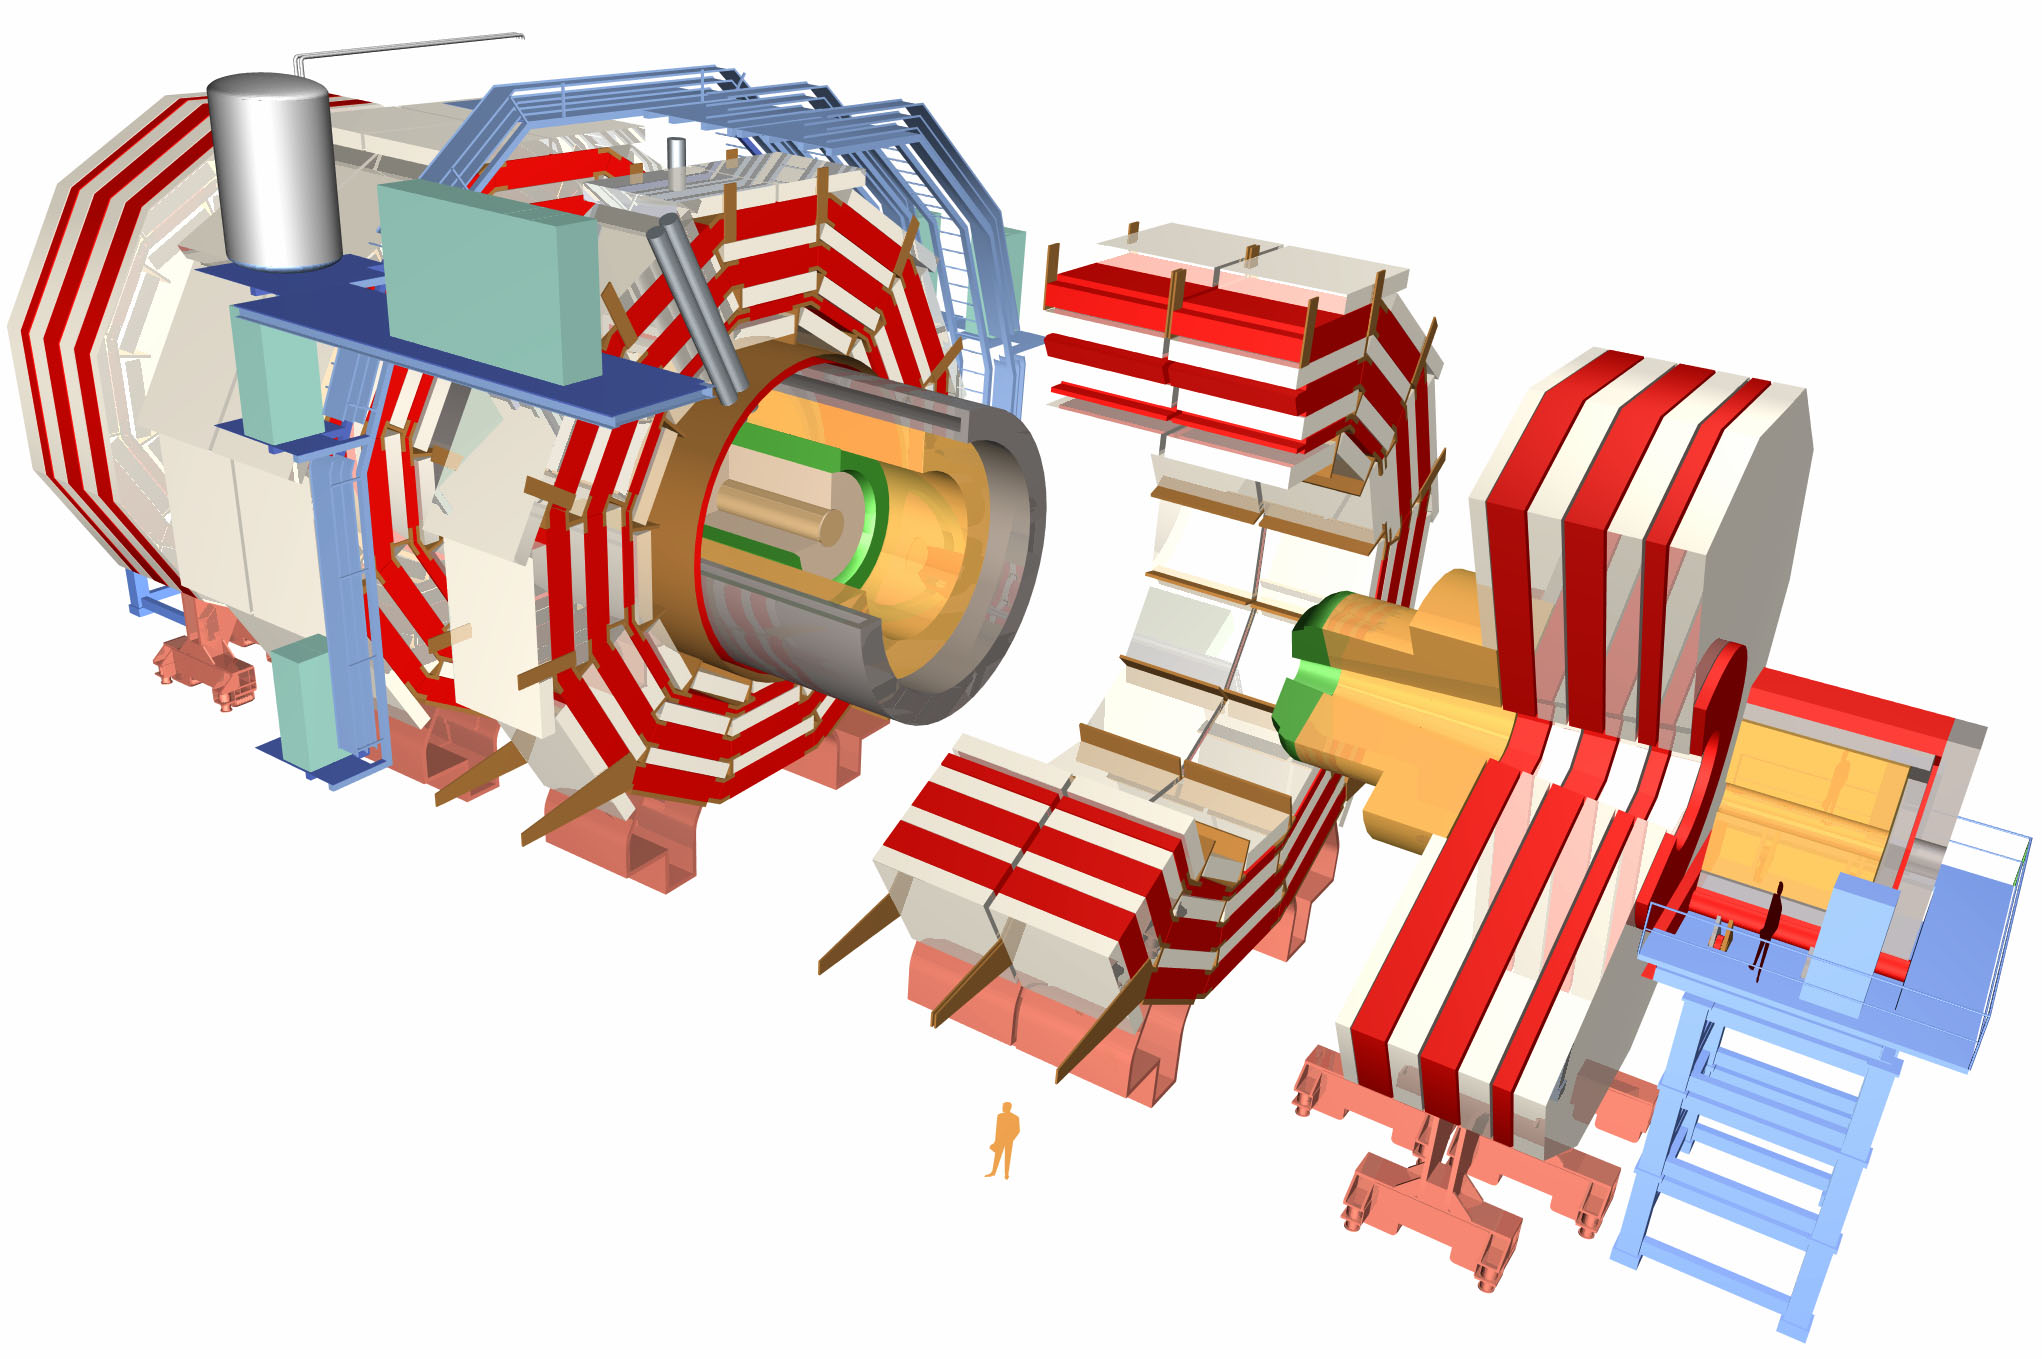
\includegraphics[width=6in]{figures/cms.jpg}
\caption{Deconstructed view of the CMS subdetectors, with human figure for scale. From inside to out, the colored segments correspond to the following systems: light brown is the pixel tracker, cream is the strip tracker, green is the EM calorimeter, orange is the hadronic calorimeter, grey is the solenoid, red is the yoke with white muon chambers. }
\label{fig:cms}
\end{figure}

\subsection{Tracking detectors}

The inner tracking detectors of CMS is supported by a 5.30 m long tube with an inner diameter of 2.38 m suspended from the HCAL barrel. The trackers contain 1,440 pixel and 15,148 strip detector modules, composing the pixel detector and silicon strip tracker, respectively. The detectors are responsible for measuring the trajectories of charged particles, essential to measuring the momenta of particles with energy $>$ 1 $\GeV$ in the range $|\eta|<2.5$, and to reconstructing secondary vertices and impact parameters, needed to identify heavy flavor particles. Being closest to the beam interaction point (IP), the tracking detectors are subjected to the highest radiation doses, and their material may interfere with the trajectories of primary particles through multiple scattering, bremsstrahlung, photon conversion, or nuclear interactions, necessitating the use of silicon technology. Additionally, due to the high particle flux of around 1,000 particles per 25 ns bunch crossing, the detectors must have both high granularity to resolve the trajectories of particles reliably and fast readout times to reduce occupancy from high flux and pileup conditions. 

\indent The detector modules of the tracking detector are shown schematically in Figure~\ref{fig:tracker}. The innermost section, labeled PIXEL, is the pixel detector, composed of 66 million 100 $\mu$m $\times$ 150 $\mu$m pixels on modules layered in three barrels at radii 4.4, 7.3, and 10.2 cm and two disks on each end at $z = \pm34.5, \pm46.5$ cm. A deconstructed barrel pixel module is shown in Figure~\ref{fig:pixmodule}, with the sensor bump-bonded onto readout chips (ROCs) controlled and powered by high-density interconnect (HDI) boards. When a charged particle passes through a pixel sensor, consisting of $n$-type pixels implanted on a high-resistance $n$-type substrate, charge carriers are induced in the conduction band of the substrate. These charge carriers then drift in the 4 T magnetic field to the nearby pixels, where an analog signal is read out, amplified, and digitized by the ROC. This drift is called charge sharing. The end cap pixel modules have a similar construction but with different pixel sensor geometries, called plaquettes. The pixel detector has a resolution of $10-40$ $\mu$m, sufficient for the imposed design requirements. 

\begin{figure}[tbh]
\centering
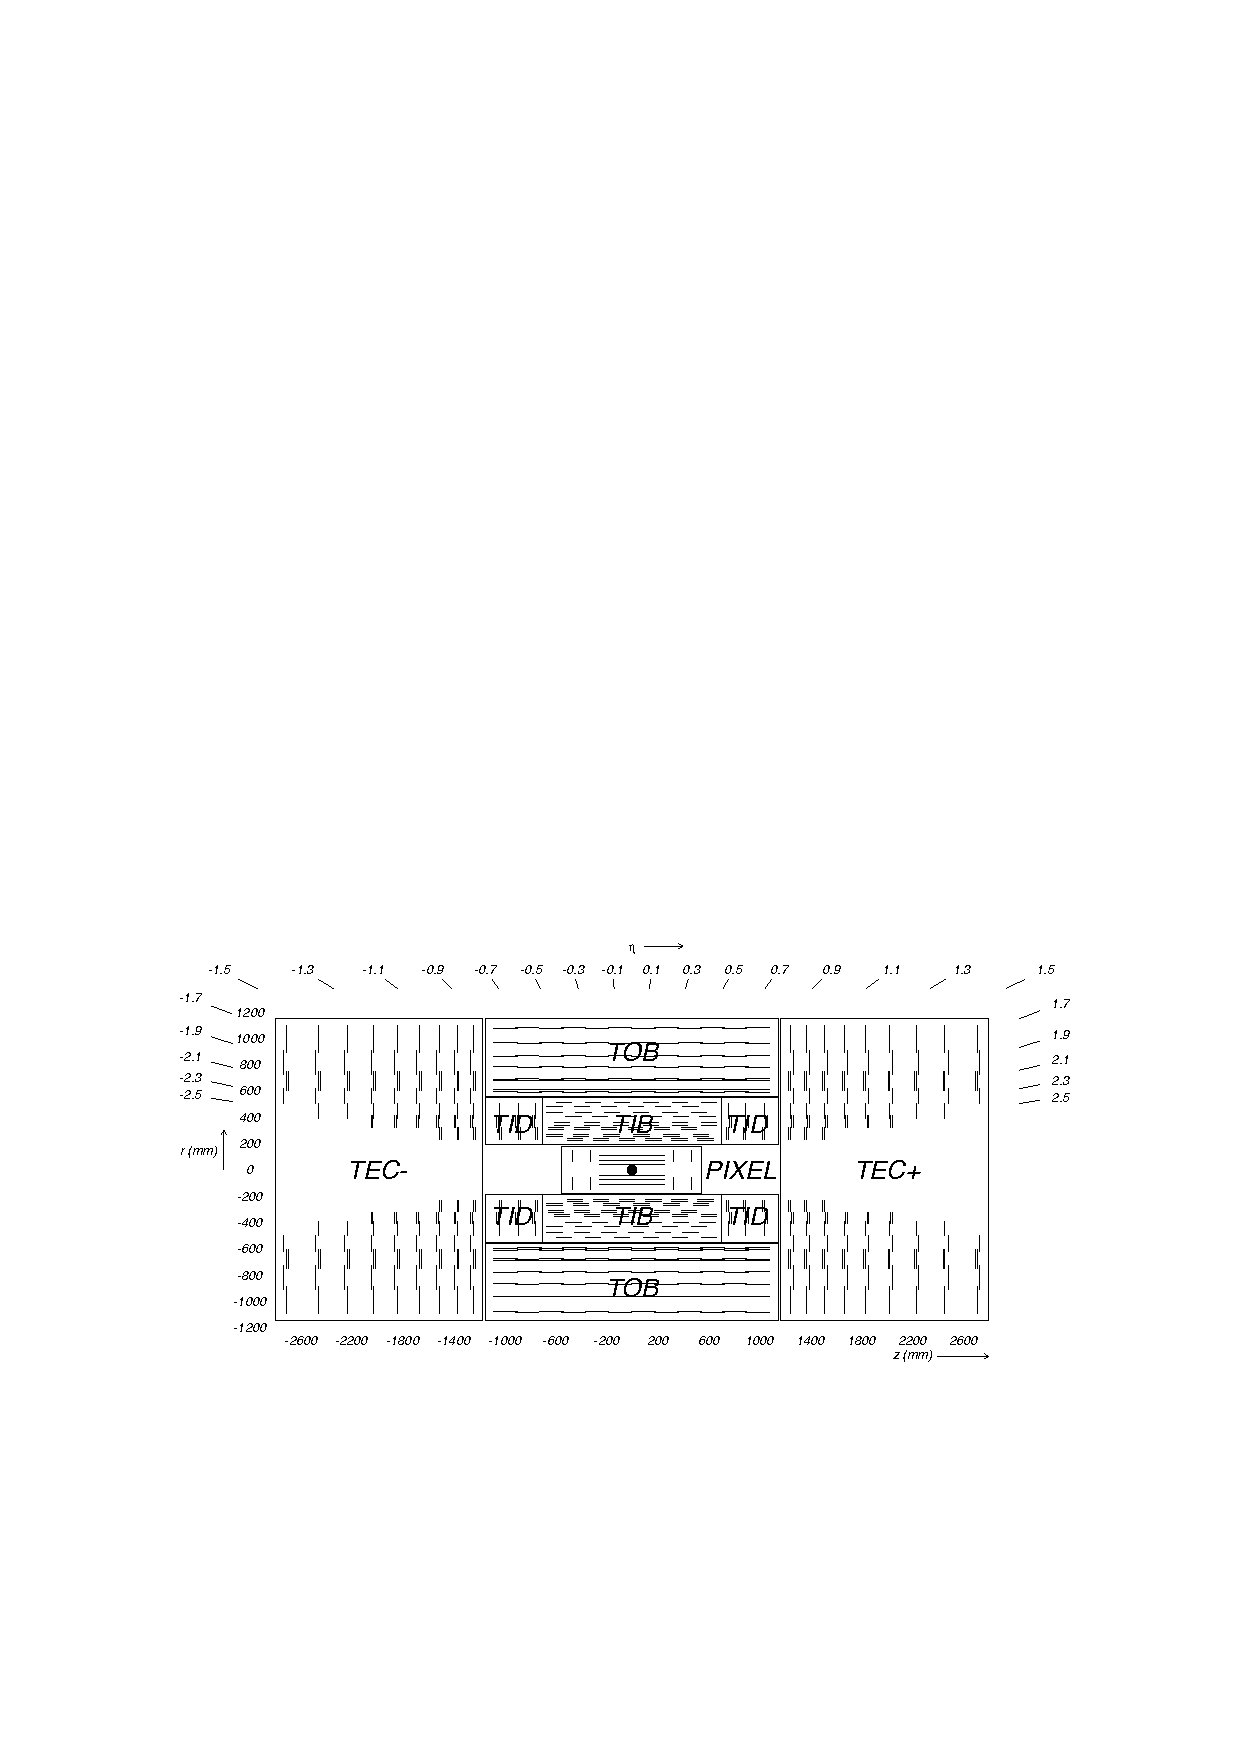
\includegraphics[width=6.5in]{figures/tracker.pdf}
\caption{Schematic diagram of tracking detectors with radial distance of modules, shown as black lines, from center on the left axis, $z$-dimension on the bottom axis, and $\eta$ accross the top.}
\label{fig:tracker}
\end{figure}

\begin{figure}[tbh]
\centering
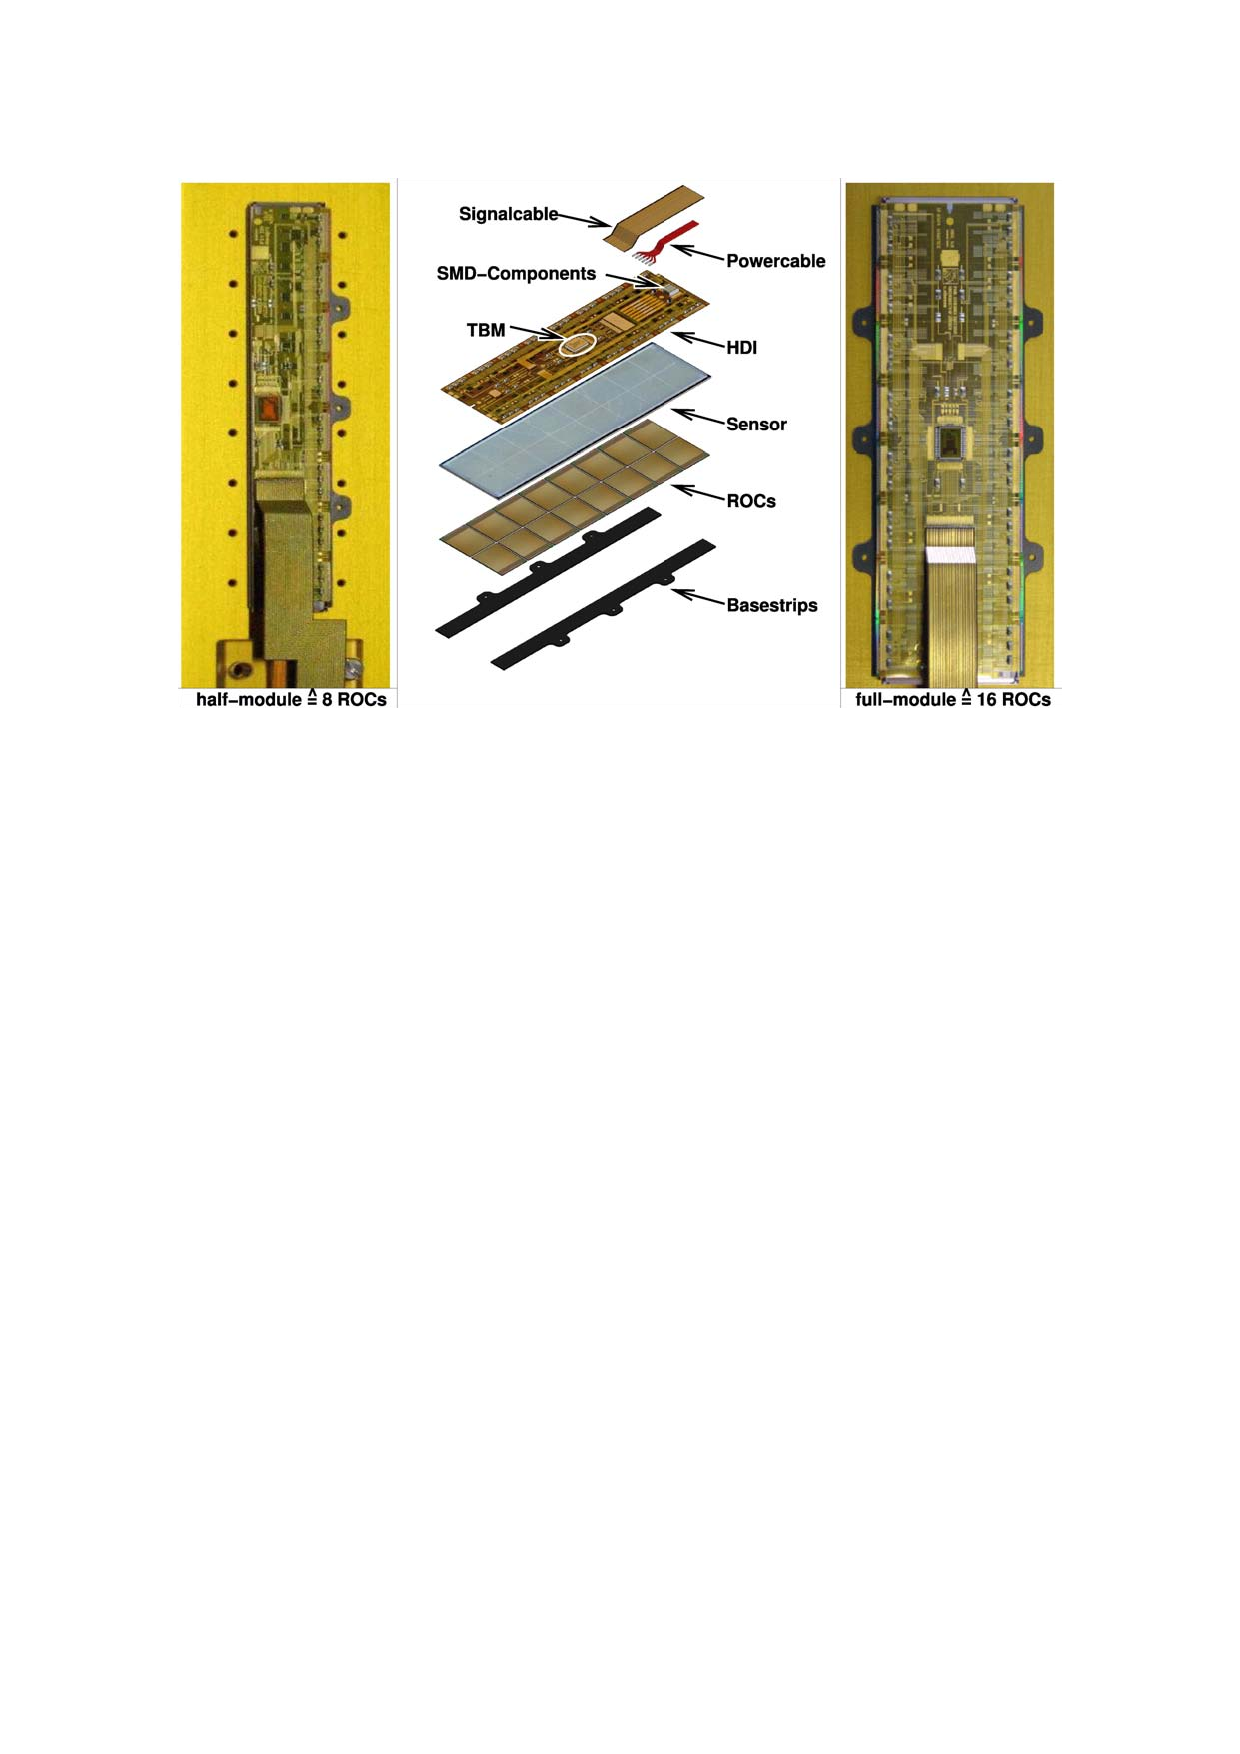
\includegraphics[width=5.5in]{figures/pixelmodule.pdf}
\caption{Deconstructed barrel pixel module showing module components.}
\label{fig:pixmodule}
\end{figure}

\indent The remaining modules of the tracking detector form the strip tracker, which fills the volume between $20-116$ cm radially, and $118$ cm in $z$. These 15,148 modules are divided into the following sections: tracker inner barrel (TIB), with four layers, tracker outer barrel (TOB) with six layers, tracker inner disks (TID) with six layers, and tracker end caps (TEC) with nine layers. The average particle occupancy at distances greater than $20$ cm from the IP is low enough compared to regions closer to the beam line that the strip tracker is not required to have the same granularity as the pixel detector, thus, twenty nine different strip module designs, of different sizes and orientations, are used. The physical principles behind the strip tracker are the same as the pixel detector: charged particles liberate conduction band electrons, which drift toward readout sensors. To enhance the effect of the charge carriers' drift in the magnetic field, the strip detectors are tilted, yielding a resolution of approximately 30 $\mu$m. Excluding defective modules, the detection efficiency of the strip tracker is nearly 100\% (Figure~\ref{fig:stripeff}) \cite{Chatrchyan:2014fea}.

\begin{figure}[tbh]
\centering
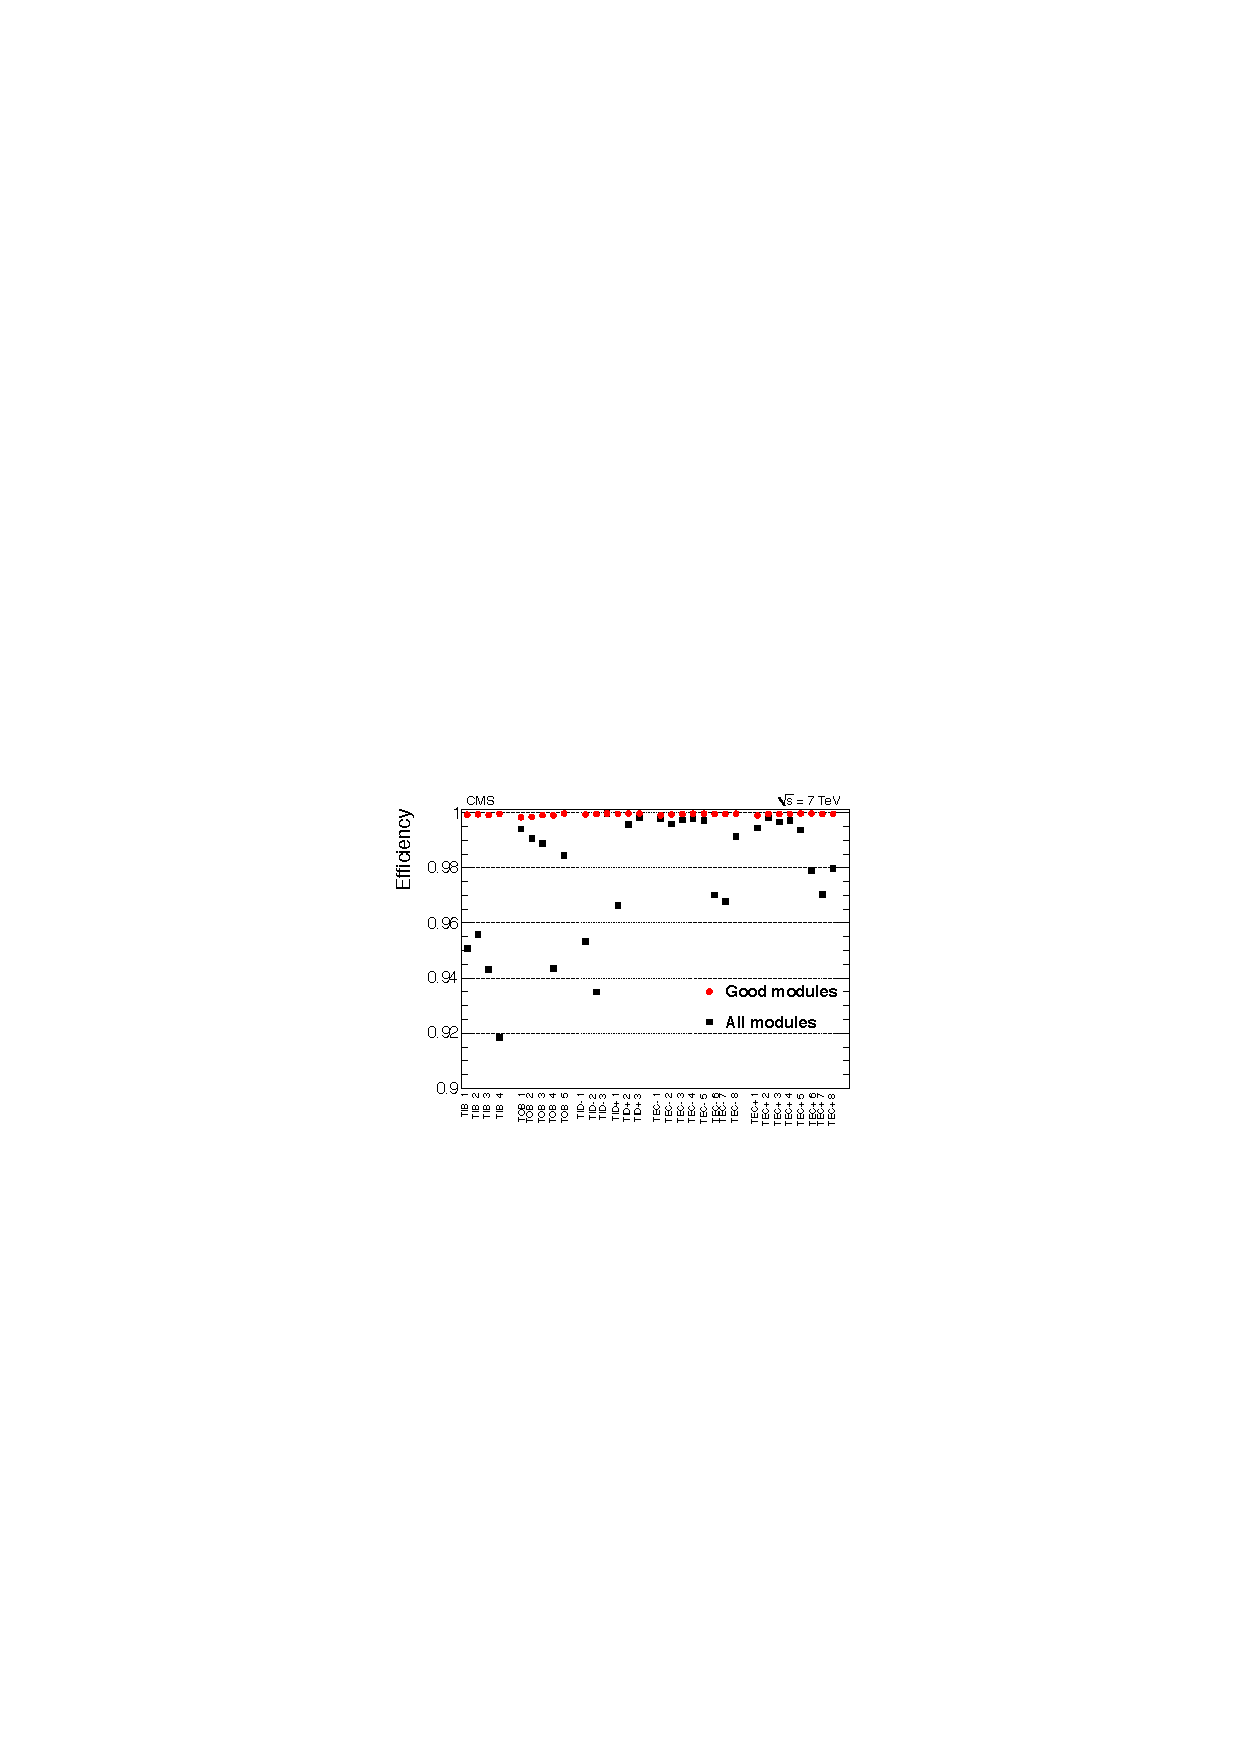
\includegraphics[width=5in]{figures/stripeff.pdf}
\caption{Average hit efficiencies of the strip tracker layers.}
\label{fig:stripeff}
\end{figure}

\subsection{Electromagnetic calorimeter}

The electromagnetic calorimeter (ECAL) consists of 61,200 lead tungstate crystal modules in the ECAL barrel (EB) region, covering $|\eta|<1.479$, and 7,324 modules in each ECAL end cap (EE), covering $1.479<|\eta|<3$. The crystals are oriented radially, as shown in Figure~\ref{fig:ecal}, at angles around three degrees in the EB and two to eight degrees in the EE from the vector to the IP to avoid cracks where particles could escape. The various supercrystal geometries are combined to form supermodules in the EB and two D-electrodes (Dees) on each end cap. The front faces of the EB crystals are at $r=1.29$ m, and present a cross section around $22$ mm$\times$$22$ mm. The EB extends to an outer radius of 1.77 m. The end cap envelopes are at $\pm315.4$ cm relative to the IP in $z$. The crystals themselves have a truncated pyramidal shape. Except for one face on the EB crystals that is depolished to account for nonuniformity in light production from the crystal shape, the crystals are polished on all sides to increase internal reflection. 

\indent The ECAL is responsible for recovering the energy of electrons and photons from the showers of scintillation light produced in the crystals. The accuracy of this measurement is of particular importance in the design of CMS, since the Higgs decay to photons and leptons are key channels in the Higgs search, one of the primary purposes of CMS. In front of each set of endcap crystals, the ECAL contains preshower detectors, consisting of a thin layer of lead followed by a thin layer of silicon strip sensors to create and detect showers from minimum ionizing particles. The primary purpose of the preshower detectors is to identify and veto neutral pion production, in addition to improving the overall position resolution of the ECAL.

\begin{figure}[tbh]
\centering
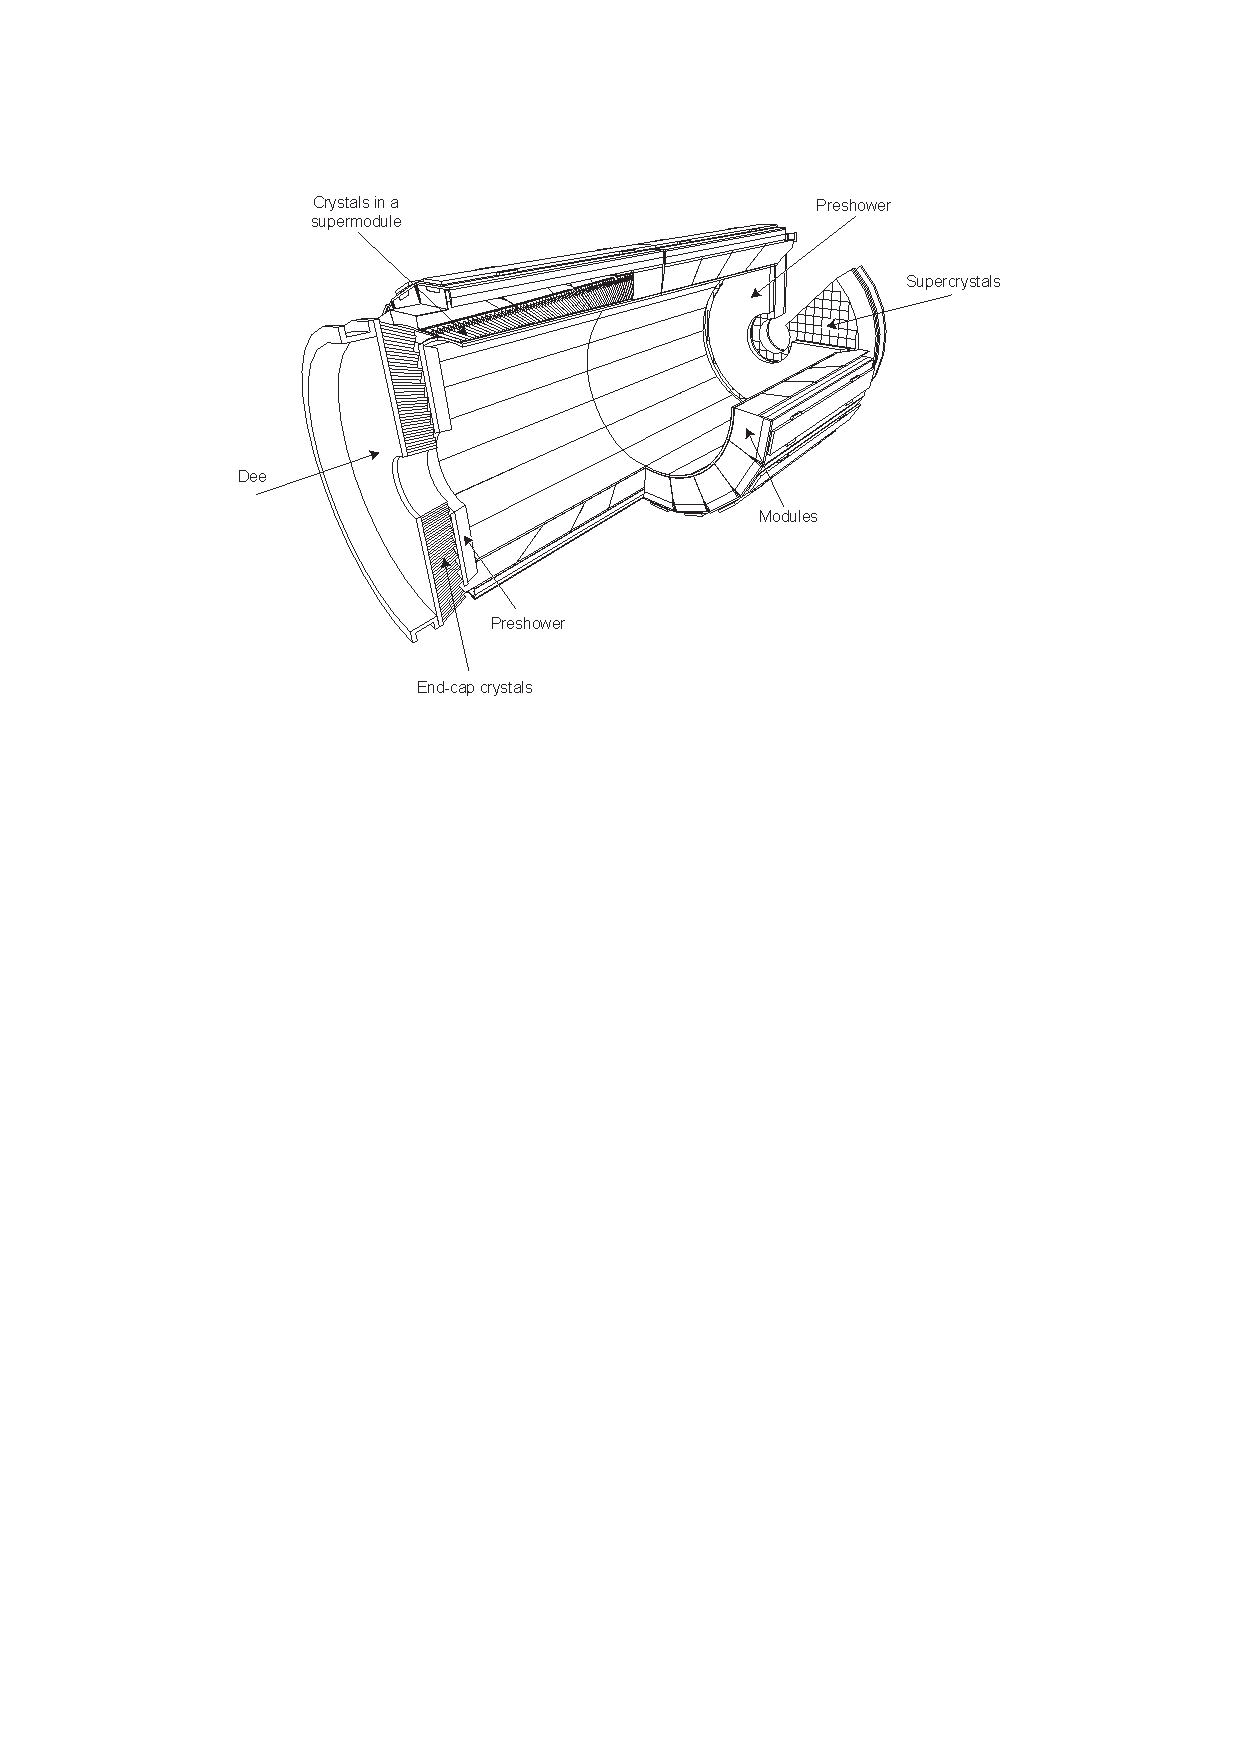
\includegraphics[width=5in]{figures/ecal.pdf}
\caption{Schematic layout of the ECAL crystal modules.}
\label{fig:ecal}
\end{figure}

\indent Lead tungstate crystals were chosen for the construction of the ECAL because of their radiation hardness. The following properties enable a compact detector with sufficiently high granularity: a high density of 8.28 g/$\rm{cm}^3$, a short radiation length of 0.89 cm, and a small Moliere radius of 2.2 cm. Additionally, the crystals have a fast scintillation decay time of about 25 ns, the same time between bunch crossings, enabling fast response and read out. At operating temperature, about 4.5 photoelectrons are collected in the attached photodetectors per $\MeV$ of incident particle energy from the blue-green scintillation light produced in the crystals. EB crystals are glued to avalanche photodiodes (APDs) while EE crystals are read by vacuum phototriodes (VPTs), each specially designed for the CMS ECAL, as shown in Figure~\ref{fig:crystalmodules}. 

\begin{figure}[tbh]
\centering
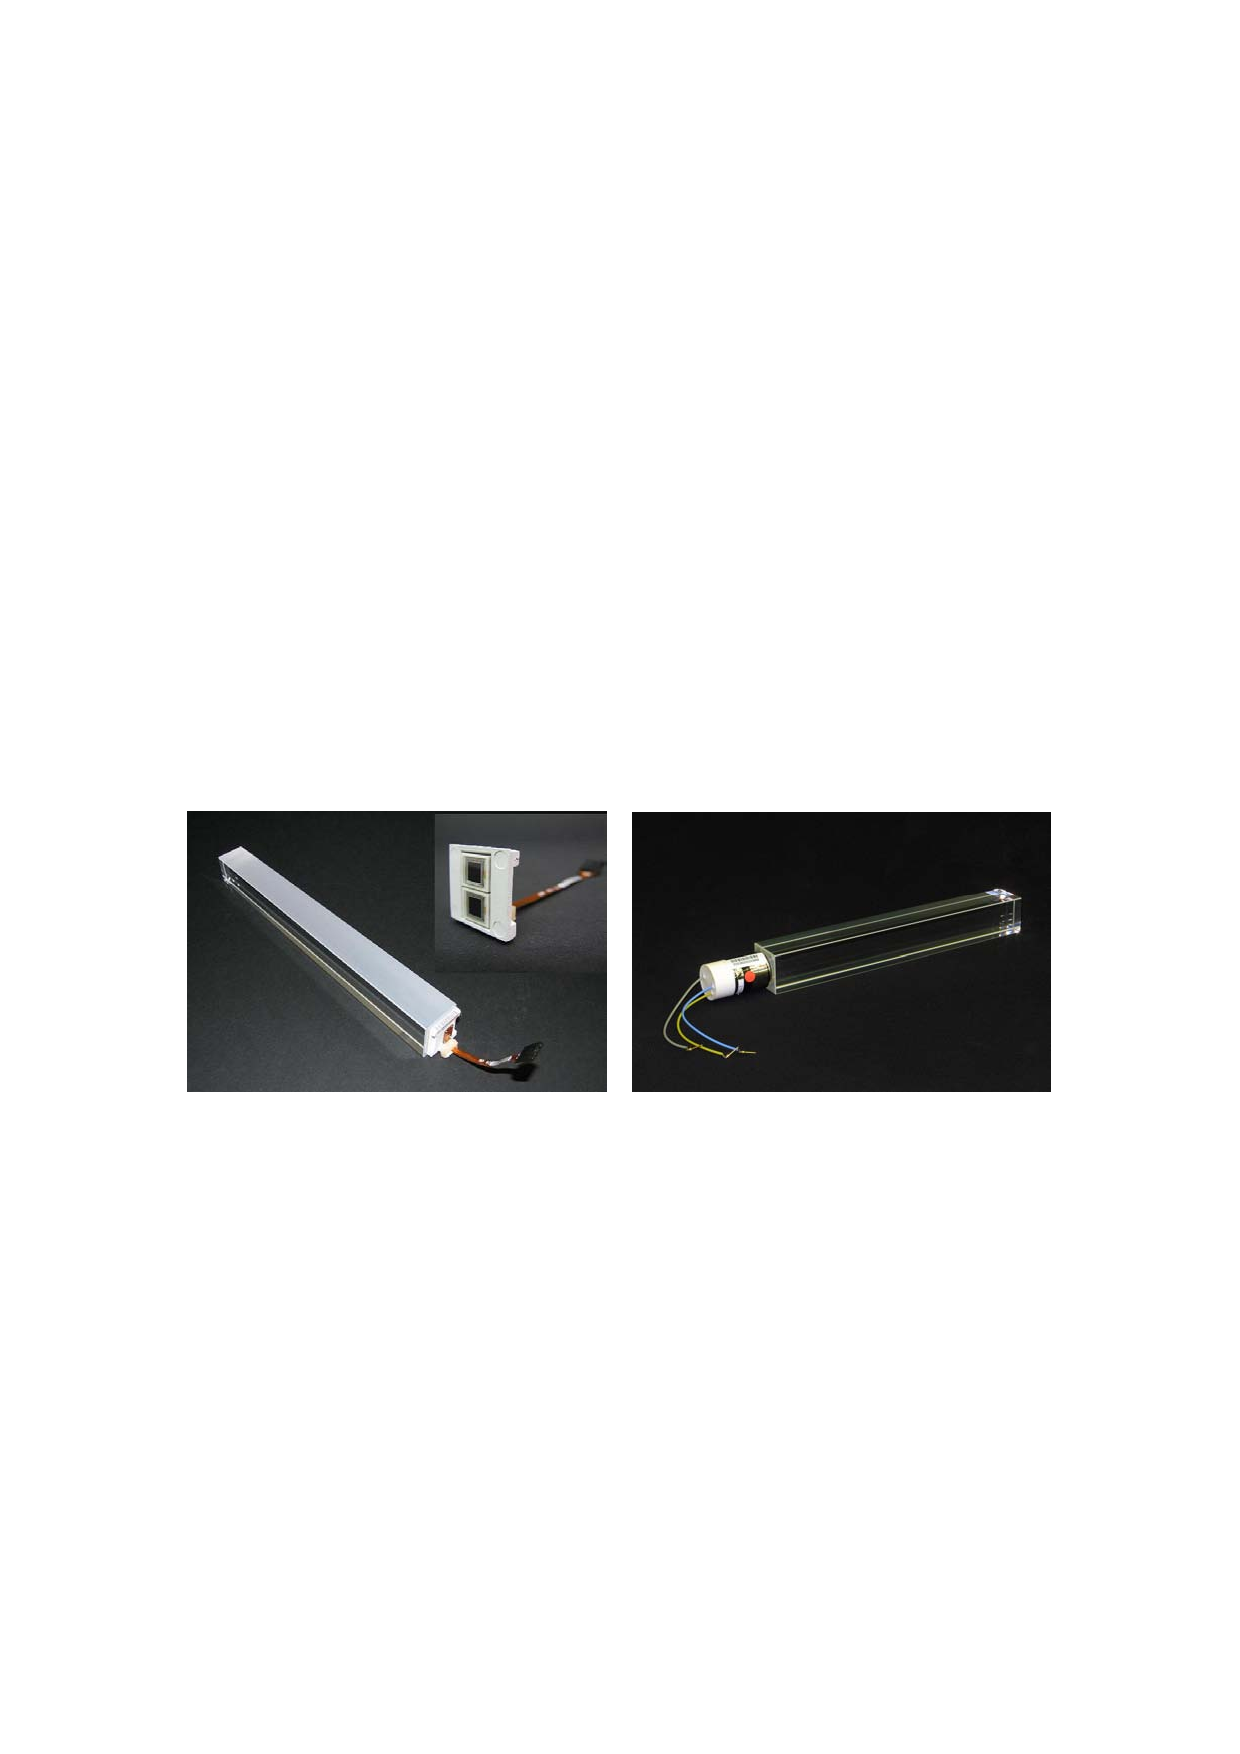
\includegraphics[width=6in]{figures/crystalmodules.pdf}
\caption{ECAL barrel crystal with one depolished face attached to avalanche photodiode photodetector (left) and ECAL end cap crystal attached to vacuum phototriode (right).}
\label{fig:crystalmodules}
\end{figure}

\indent The energy resolution of the ECAL depends on the energy of the incident particle, and can be parametrized as the sum of three terms:
\begin{equation}
\bigg(\frac{\sigma}{E}\bigg)^2 = \bigg(\frac{S}{\sqrt{E}}\bigg)^2 + \bigg(\frac{N}{E}\bigg)^2 + C^2
\end{equation}
The first term, called the stochastic term, arises from fluctuations in the lateral shower containment, photostatistics, and fluctuations in energy deposited in the preshower detector. The second term, called the noise term, arises from electronic, digitization, and pileup noise. The third term, called the constant term, arises from nonuniformity in light collection, calibration errors, and leakage from the back of the crystals. Test beam experiments using electron beams with momenta $20-250$ $\GeV$ found approximate values for the parameters: $S=0.028$, $N=0.12$, and $C=0.003$. 

\subsection{Hadronic calorimeter}

The hadronic calorimeter (HCAL) lies primarily within the bore of the CMS solenoid, surrounding the ECAL, between 1.77 m and 2.95 m from the beam line, covering up to $|\eta|<5.2$. The HCAL is divided into four subsystems, shown schematically in Figure~\ref{fig:hcal}: the HCAL barrel (HB) region, covering $|\eta|<1.3$, the HCAL end caps (HE), covering $1.3<|\eta|<3$, the HVAL outer (HO) calorimeter, or tail catcher, double covering the EB and HB regions to ensure complete shower absorption, outside the solenoid, and the HCAL forward (HF) calorimeter, covering up to $|\eta|<5.2$ at 11.2 m from the IP. The primary function of the HCAL is to measure the energy and direction of hadronic jets, showers of particles produced from particles composed of quarks and gluons interacting with the detector material. Another important function of the HCAL is to contribute to the measurement of MET, which is a key variable in this analysis. 

\begin{figure}[tbh]
\centering
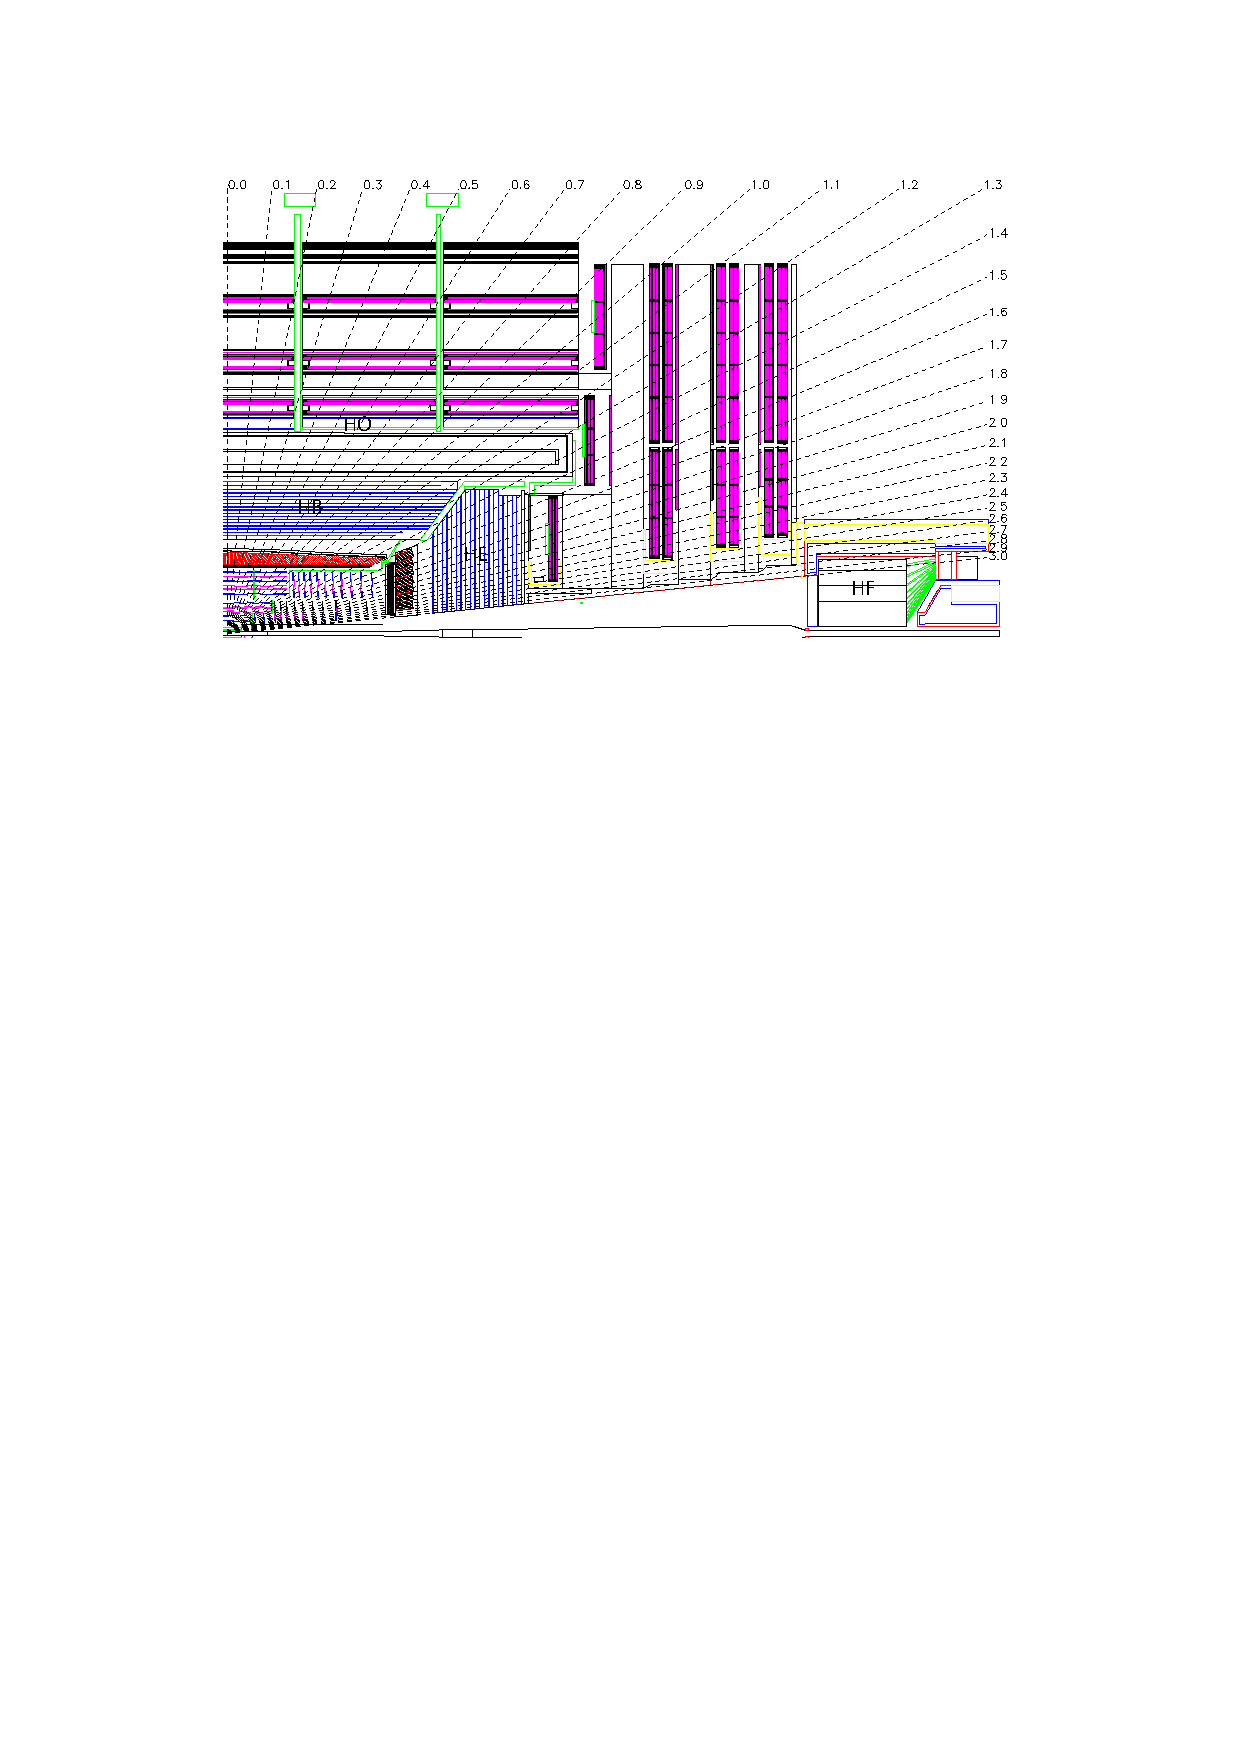
\includegraphics[width=6in]{figures/hcal.pdf}
\caption{Cross sectional view of one quadrant of CMS. The labeled sections are the subsytems of the hadronic calorimeter.}
\label{fig:hcal}
\end{figure}

\indent The HCAL subsystems consist of layers of absorber material and scintillator material. The absorber material causes incident hadrons to shower into quarks and gluons, whose energy is deposited and read out from the scintillator layers. Tiles of scintillator material are organized into units called trays. The HB consists of two half-barrels, each with eighteen identical $\phi$-wedges, each consisting of seventeen layers of scintillator material, with each layer containing 108 trays. The scintillator layers are separated by eight 50.5 mm thick and six 56.5 mm thick brass plates and surrounded by an inner 40 mm thick and outer 75 mm thick steel plate. The HE disks consist of 36 identical $\phi$-wedges, with a total of 1,368 trays of 20,916 trapezoidal scintillator tiles divided into 18 layers, alternating with 79 mm thick brass plates. The HO layers are each divided into 12 $\phi$-sectors, consist of 40 mm thick detector layers of scintillator and aluminum supports, layered into the 75 mm thick steel beams of the return yoke. The HB, HE, and HO tiles are arranged to attain a granularity of $(0.087, 0.087)$ in $(\eta, \phi)$. The scintillation light produced in the HB, HE, and HO tiles is collected by wavelength-shifting (WLS) fibers, grouped by tray in clear fibers leading to optical decoders which arrange the clear fibers into readout towers, transmitted to hybrid photodiodes (HPD) for amplification and readout. The energy resolution of HB+HE versus HB+HE+HO systems for test beam pions is shown in Figure~\ref{fig:eres_hcal}, with a clear improvement when including the HO.

\begin{figure}[tbh]
\centering
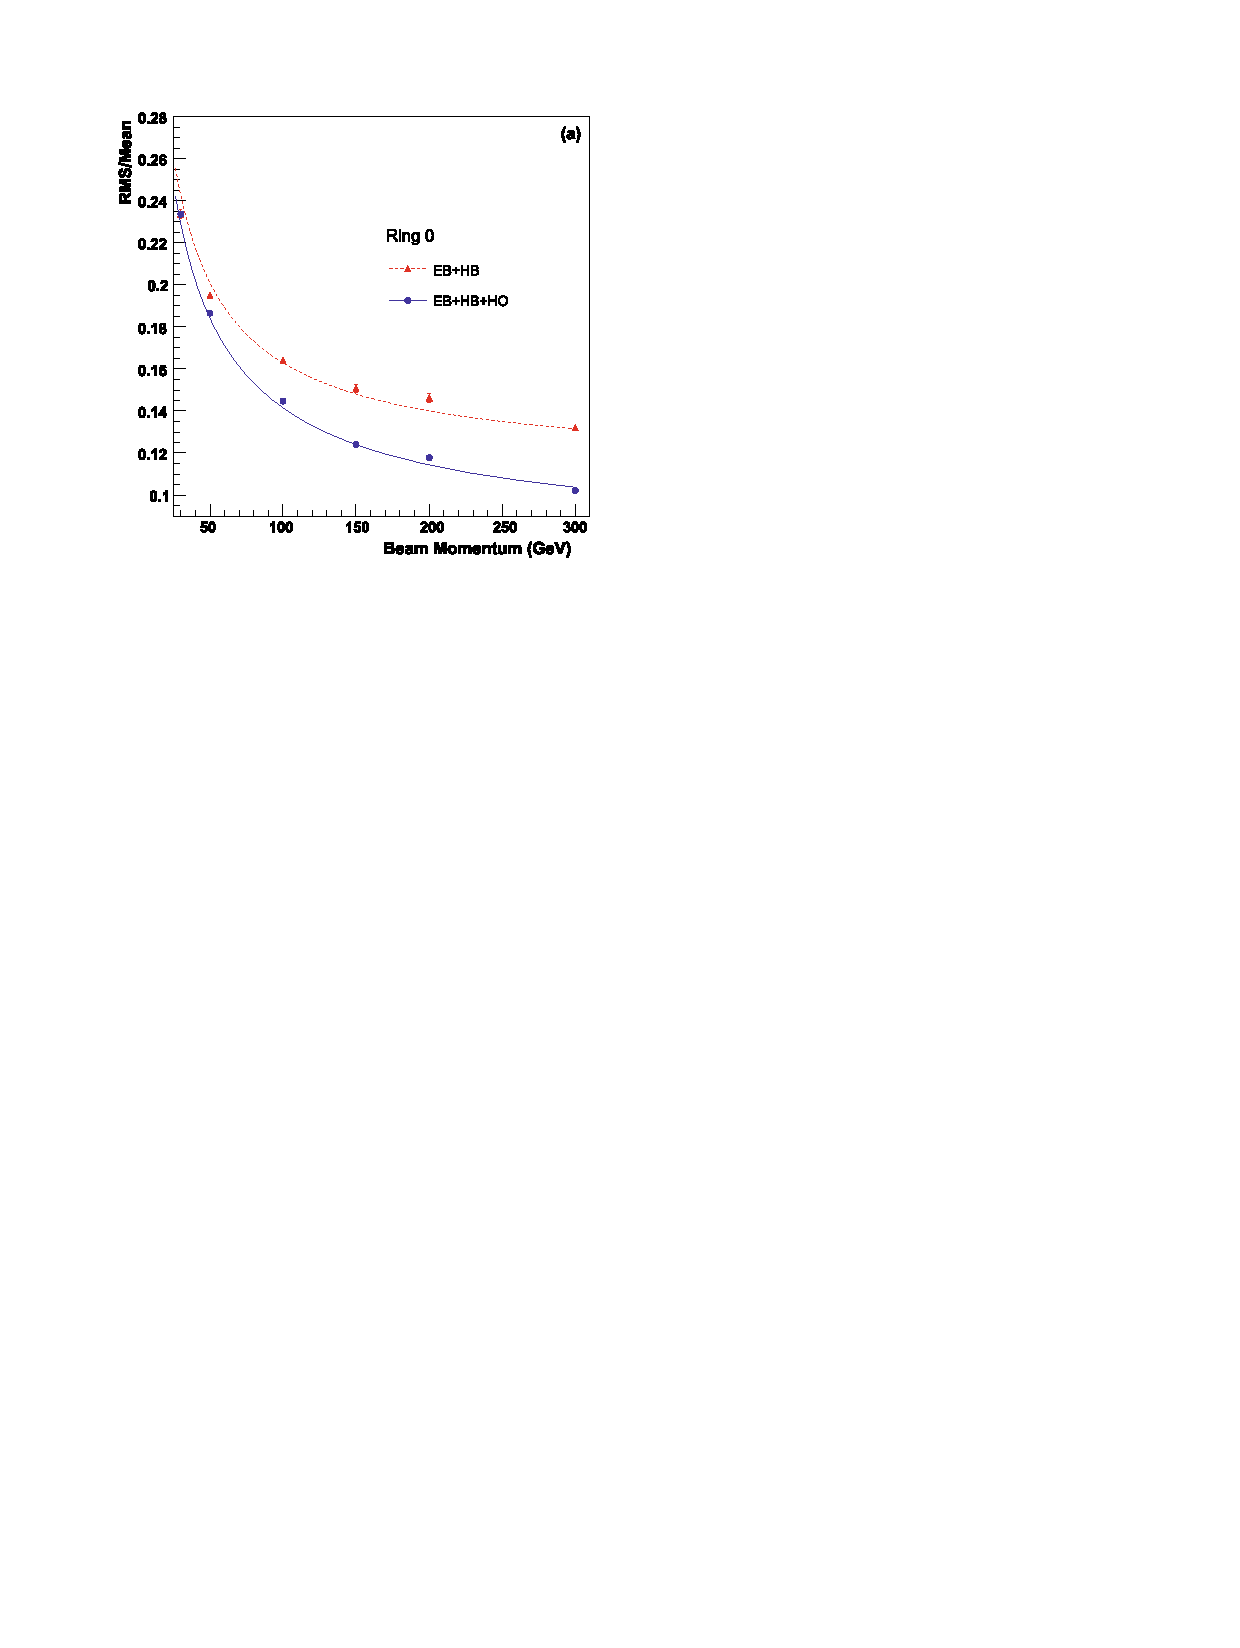
\includegraphics[width=4in]{figures/eres_hcal.pdf}
\caption{Energy resolution of HCAL systems for test beam pions.}
\label{fig:eres_hcal}
\end{figure}

\indent The HF barrels consist of eighteen identical $\phi$-wedges, with layers of 5 mm thick steel plates. Due to higher radiation doses, quartz fibers are used instead of plastic as in the other HCAL subsystems to produce scintillation light. The quartz fibers lie in grooves cut in the steel plates, with half running the full length of the absorber and half starting 22 cm, from the front of the HF barrel. This can be used to classify showers as EM or hadronic, as EM showers deposit most of their energy in the first 22 cm while hadronic showers deposit roughly the same energy throughout the material. Fibers are bundled into towers with a granularity of $(0.175, 0.175)$. Additionally, the HF is used to measure the luminosity of the LHC beam.

\subsection{Muon detectors}

As muons are able to pass through the inner detector material with little radiative losses, the CMS muon system is the outermost subdetector system, consisting of end caps and a barrel region divided into four layers called stations. The barrel region is segmented into regions based on the five 2.536 m yoke rings at $z = 0, \pm5.342, \pm2.686$ and the iron ribs of the yoke support structure. With the goal of reconstructing the momenta and charge of muons over a wide angular and kinematic range, three types of gas-ionization detection mechanisms are employed: drift tubes (DTs), cathode strip chambers (CSCs), and resistive plate chambers (RPCs). 

\indent The barrel DT system consists of drift cells, 13 mm $\times$ 42 mm $\times$ 2.4 m chambers filled with 85\% Ar and 15\% $\rm{CO}_2$ gas, with outer cathode strips and an inner anode wire to read out charge carriers ionized when a charged particle passes through the gas. Four drift cells are stacked, staggered by half a cell, to form superlayers (SLs). SLs are combined in groups of two or three to form drift chambers. The inner three stations have sixty DT chambers, with cells having anode wires running in the $r-\phi$ and z directions. The outer station has seventy DT chambers with cells having anode wires running only in the $r-\phi$ direction. A schematic diagram of the layout of the DT chambers, layered in the iron yoke, is shown in Figure~\ref{fig:DTs}.

\begin{figure}[tbh]
\centering
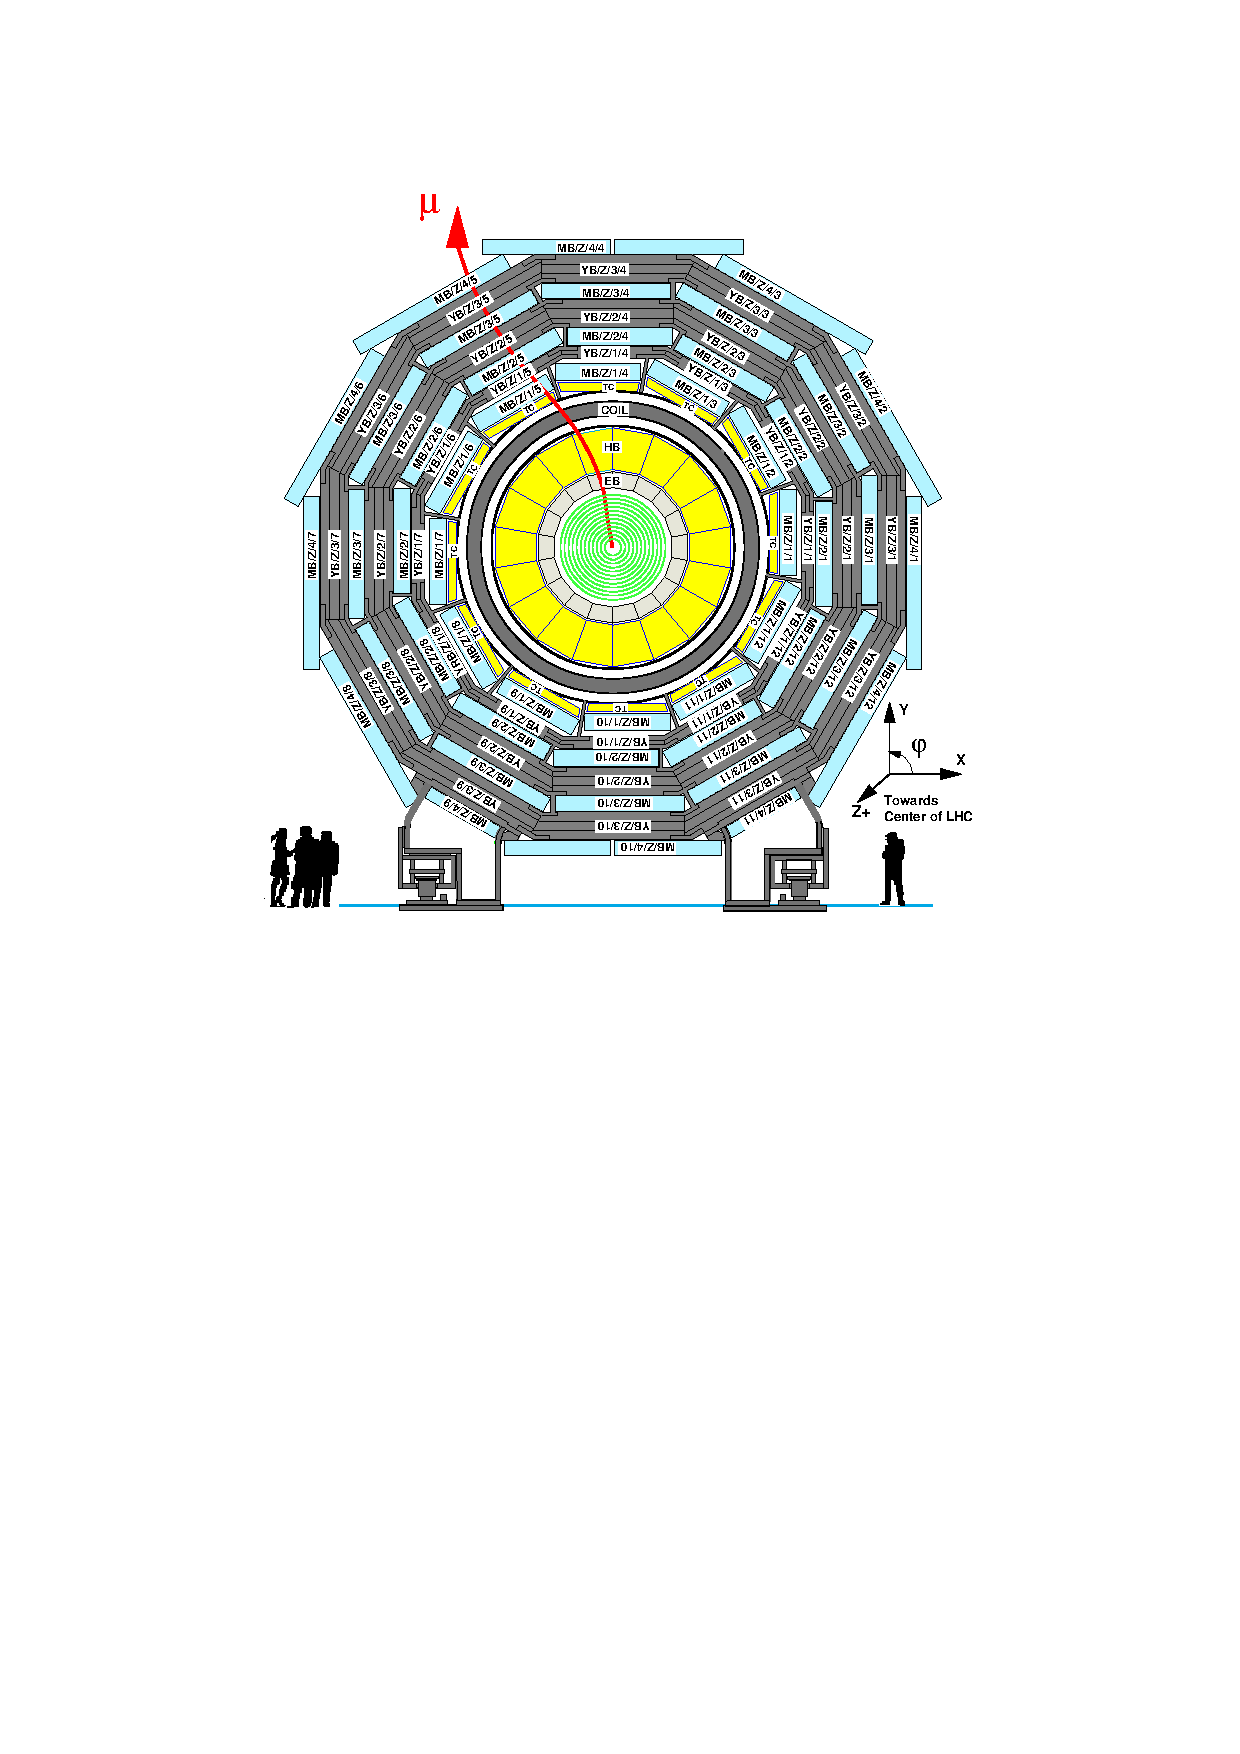
\includegraphics[width=5in]{figures/DTs.pdf}
\caption{Schematic diagram showing DT chambers in light blue.}
\label{fig:DTs}
\end{figure}

\indent The end cap CSC system consists of 468 trapezoidal CSC modules, proportional counters with six azimuthal anode wires running perpendicular to seven radial cathode strips, providing measurements of $r$ and $\phi$ with $80 \mu$m resolution with pseudorapidity coverage $0.9 < |\eta| < 2.4$. Muons passing though the chambers' 40\%:50\%:10\%, Ar:$\rm{CO}_2$:$\rm{CF}_4$ gas mixture produce an avalanche of positively charged carriers, whose signals are interpolated across multiple cathode strips along the anode wires to reconstruct the avalanche position. The position of the CSCs in a cutout quadrant of CMS is shown in Figure~\ref{fig:cscs}.

\begin{figure}[tbh]
\centering
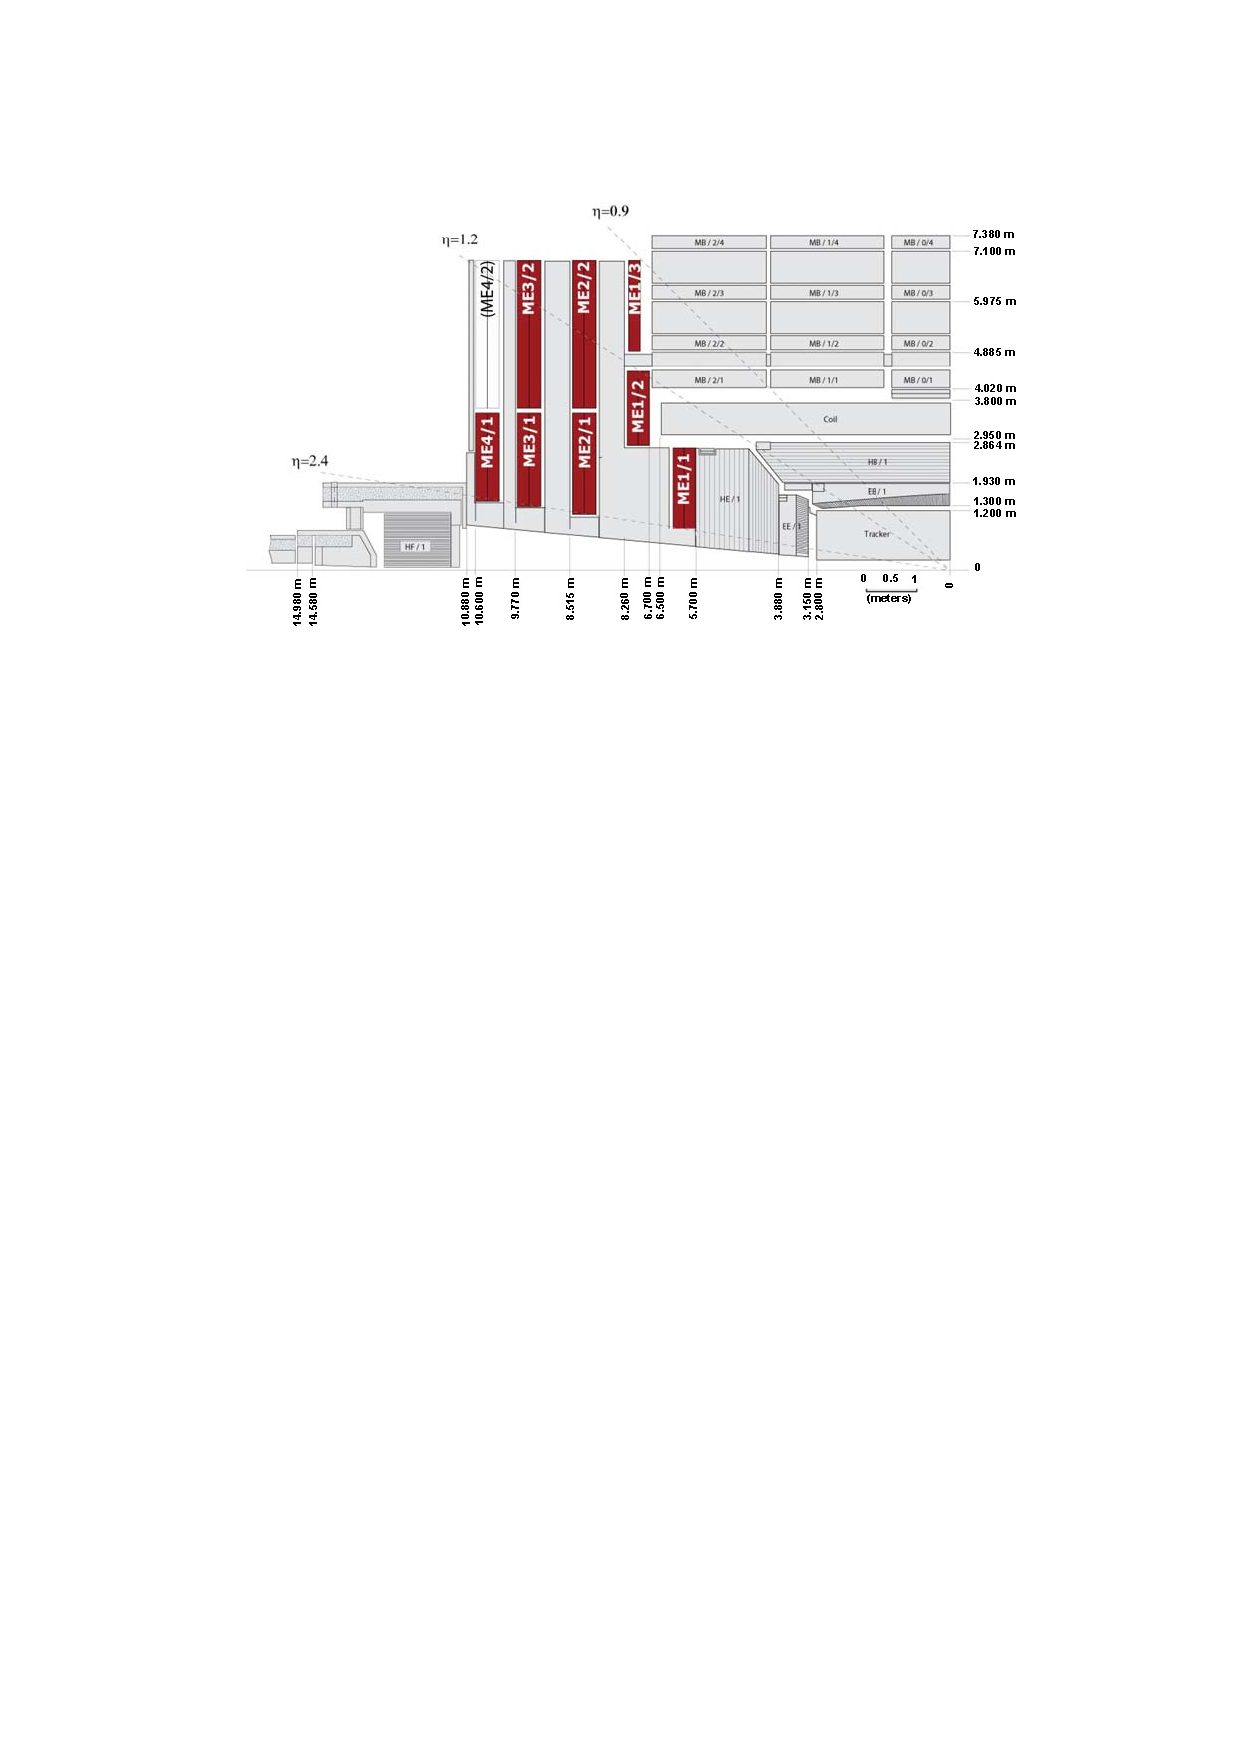
\includegraphics[width=4in]{figures/cscs.pdf}
\caption{Schematic diagram showing CSC locations in red in a quadrant cutout of CMS.}
\label{fig:cscs}
\end{figure}

The final muon subsystem, the 480 rectangular barrel and trapezoidal end cap RPCs, are arranged in six barrel layers, two in stations one and two, and one each in stations three and four, and in three layers in each end cap. The RPC modules contain parallel-plate detectors with $2-3$ double-gap modules of up to 96 (32) strips, parallel (radial) to the beam line in the barrel (end cap) sections, which collect ionized charge carriers from the 96.2\%:3.5\%:0.3\%, $\rm{C}_2\rm{H}_2\rm{F}_4$:$\rm{C}_4\rm{H}_{10}$:S$\rm{F}_6$ gas. A schematic of the module layout is shown in Figure~\ref{fig:rpcs}. The timescale in which RPCs can tag events is faster than the 25 ns bunch crossing time of the LHC, which in combination with the other muon systems, allows efficient triggering on muon events, discussed further in the next section.

\begin{figure}[tbh]
\centering
\begin{subfigure}{0.45\textwidth}
\centering
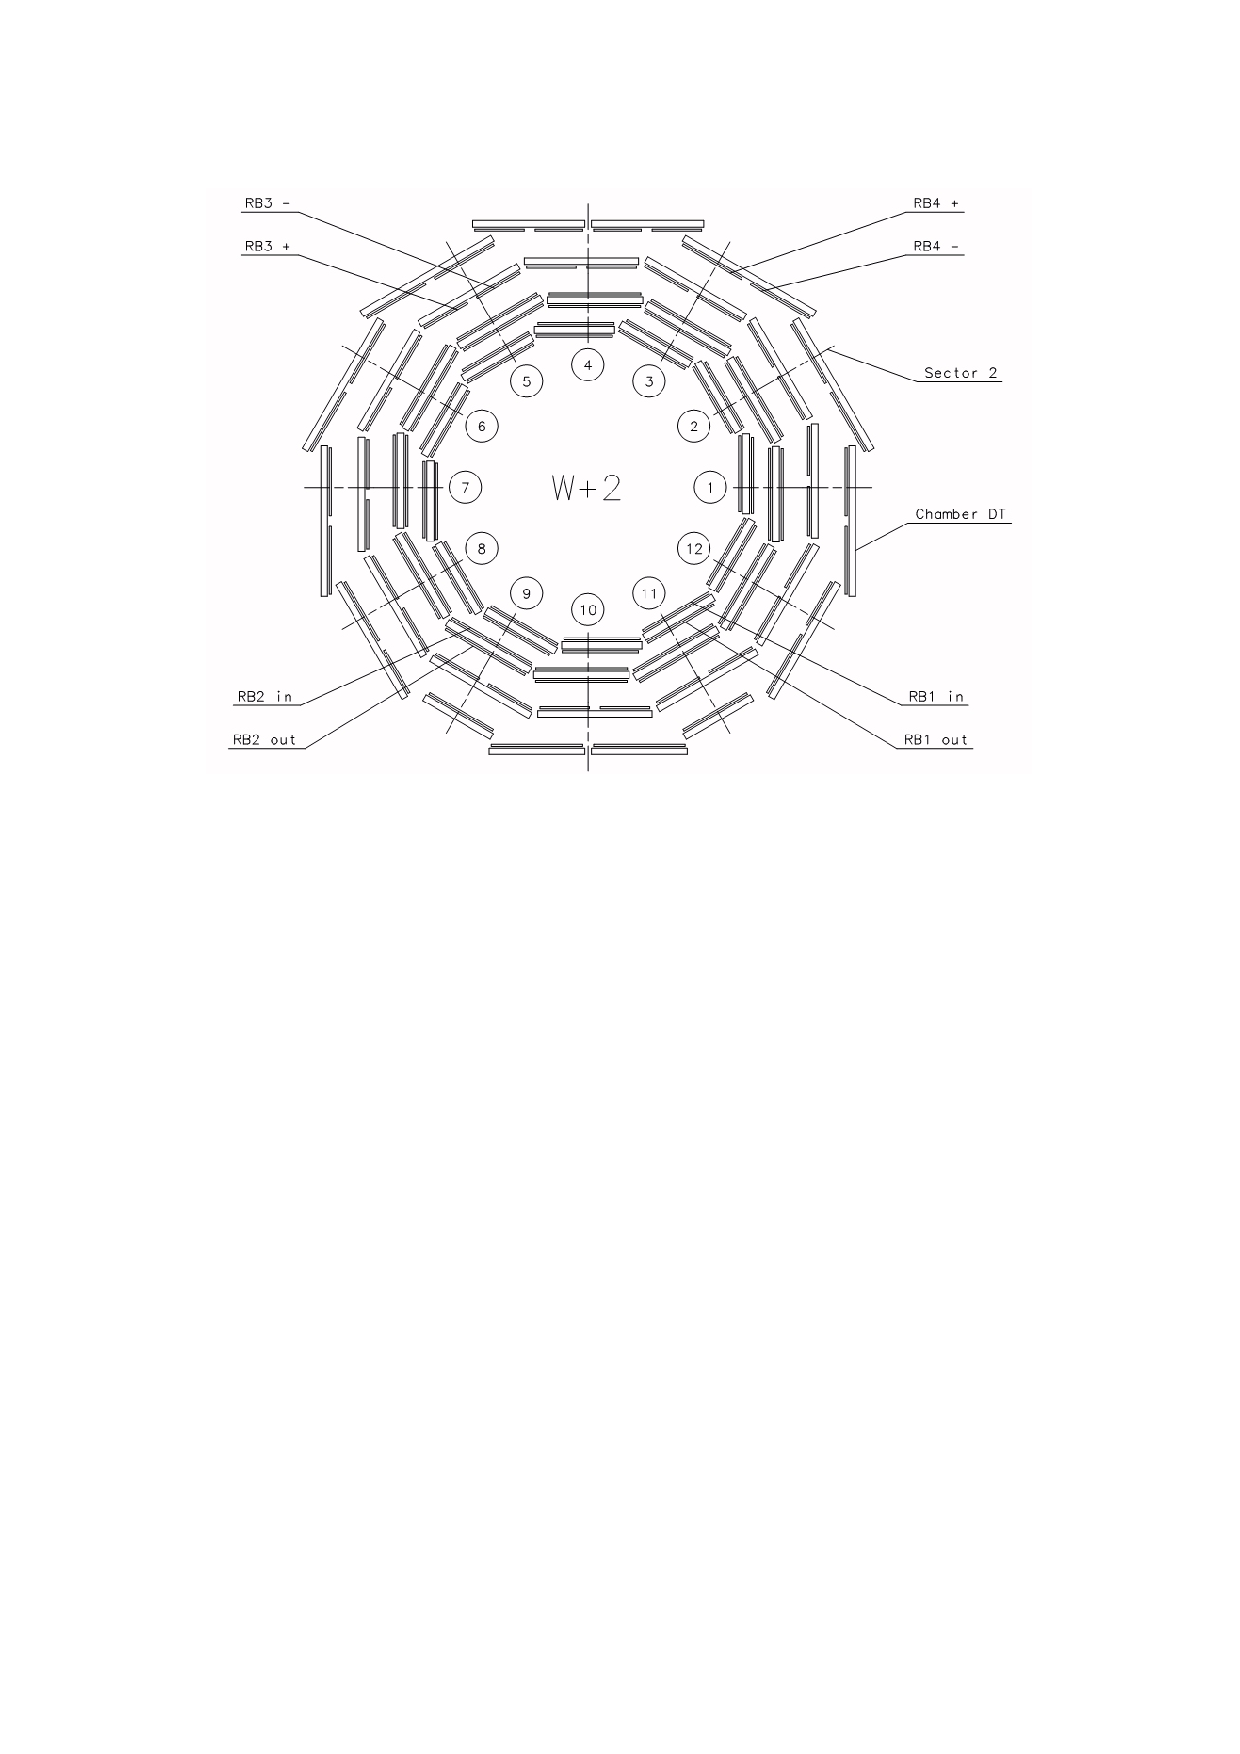
\includegraphics[width=3in]{figures/rpcbarrel.pdf}
\caption{}
\end{subfigure}
\begin{subfigure}{0.45\textwidth}
\centering
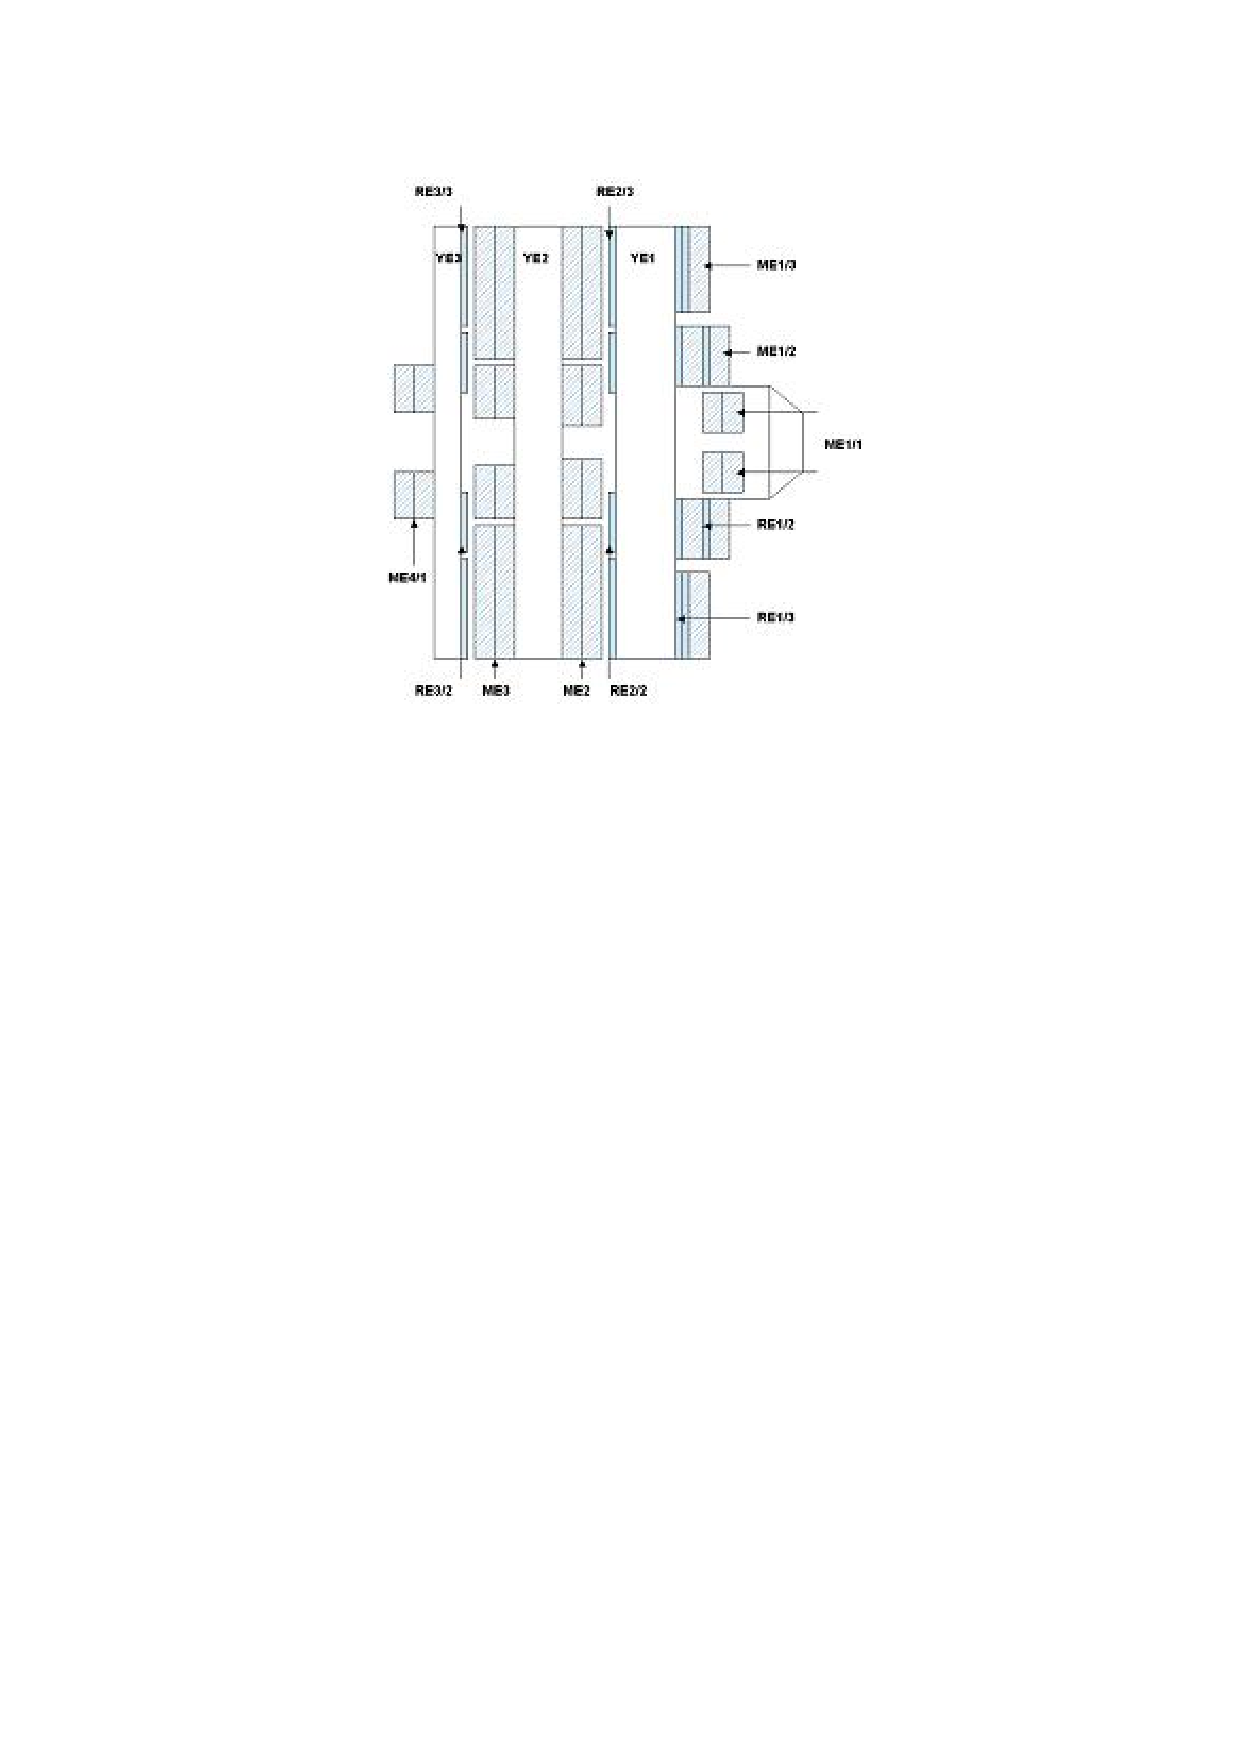
\includegraphics[width=3in]{figures/rpcendcap.pdf}
\caption{}
\end{subfigure}
\caption{Schematic diagram showing barrel RPC locations (left) and end cap RPCs (right) in a cross sectional cutout of CMS.}
\label{fig:rpcs}
\end{figure}

\indent The objective of the muon system to accurately measure the momenta of muons over a wide pseudorapidity range is accomplished, as shown by the less than 6\% transverse momentum resolution shown in Figure~\ref{fig:muonres} \cite{1748-0221-7-10-P10002}.

\begin{figure}[tbh]
\centering
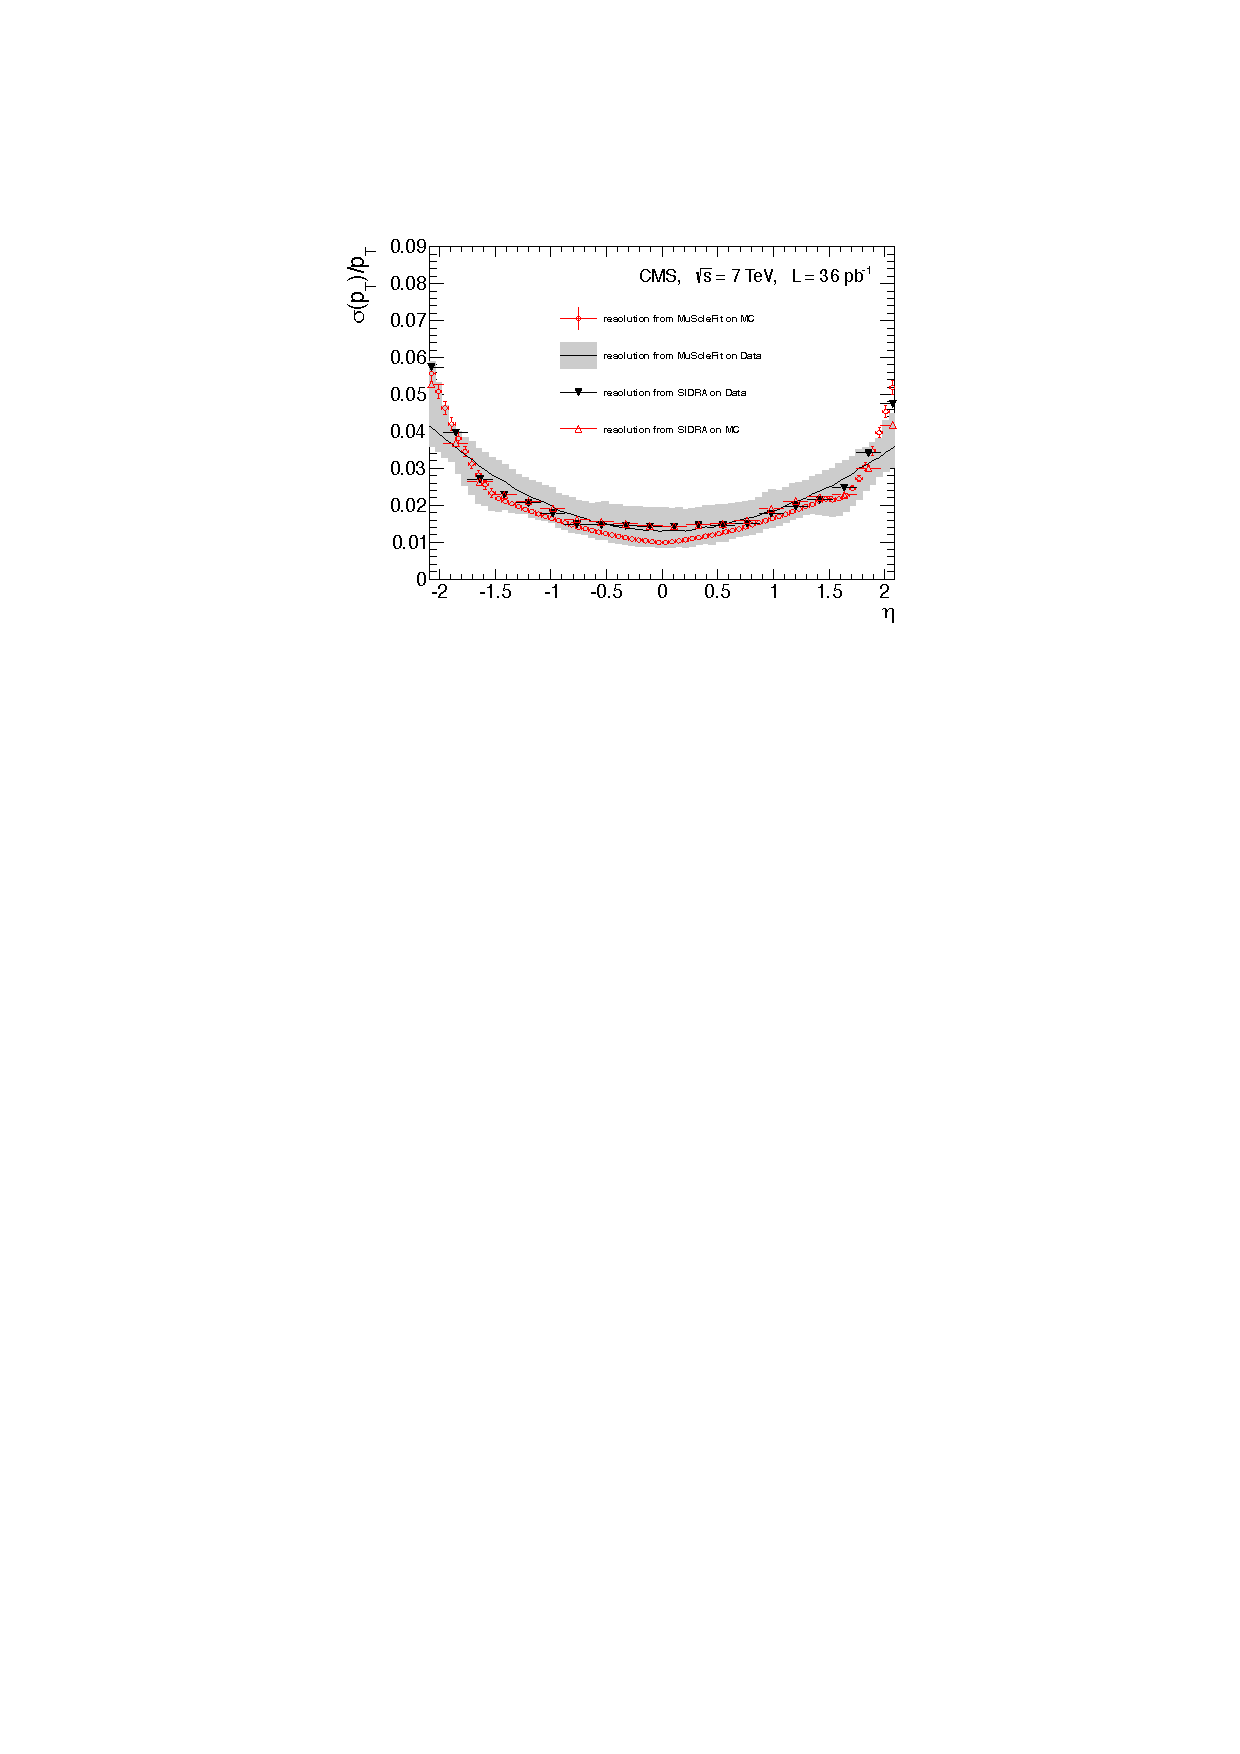
\includegraphics[width=5in]{figures/muonres.pdf}
\caption{Transverse momentum resolution versus pseudorapidity for muons from $Z$ decays.}
\label{fig:muonres}
\end{figure}

\subsection{Trigger}

In order to reduce the O(100) MHz interaction rate from LHC proton collisions to a computationally manageable O(100) kHz rate, a trigger system consisting of an Level-1 Trigger (L1T) and a High-Level Trigger (HLT) is employed. The L1T, summarized in Figure~\ref{fig:l1t}, uses mainly field programmable gate array (FPGA) technology on the front-end electronics to compile local trigger primitives from calorimeter towers and muon tracks into regional triggers, which use pattern logic to identify objects like electrons and muons. The highest quality objects are piped to the global trigger, which decides, based on further calculations and input on the status of the subdetectors, whether an event is rejected or an L1 Accept signal is sent to the Timing, Trigger, and Control (TTC) system for reading out the front-end data buffers, with a latency of 3.2 $\mu$s.

\begin{figure}[tbh]
\centering
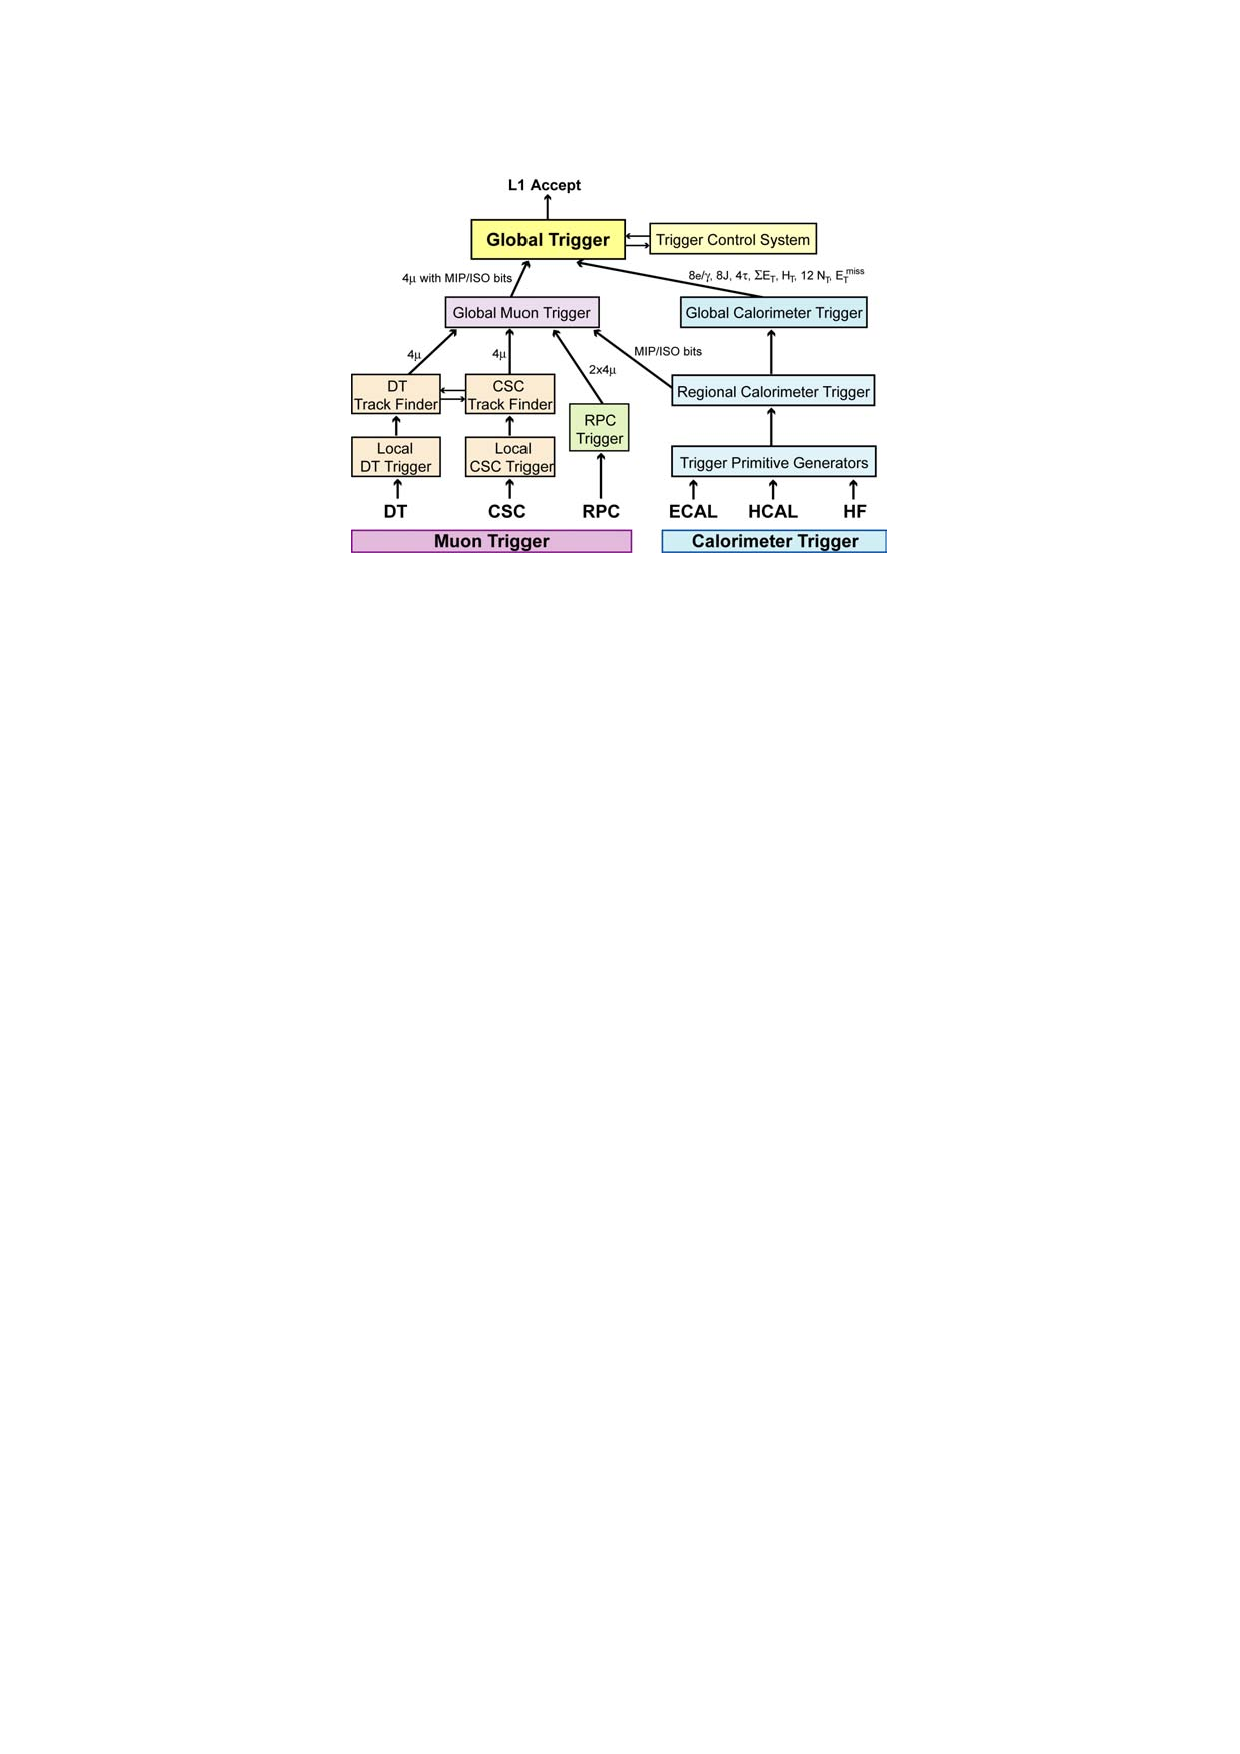
\includegraphics[width=5in]{figures/l1t.pdf}
\caption{CMS L1 trigger system schematic diagram.}
\label{fig:l1t}
\end{figure}

\indent After an event passes the L1T, the entire event data is read out by the data acquisition (DAQ) system, summarized in Figure~\ref{fig:daq}. First, data is read out from the subdetector front-end buffers to the front-end drivers (FEDs), followed by the merging of FED fragments by the Event Builder and the submission of the complete event data to the HLT by the Event Filter. The HLT is a software system, which uses filtering and reconstruction algorithms to select events based on their physics object content, with different paths based on the different combinations of objects used in physics analyses. The HLT paths used in this analysis are based on combinations of high quality lepton objects, such as two muons or two electrons, and are discussed further in the next chapter. Data quality monitoring (DQM), is also carried out at this step, to ensure all subsystems are behaving properly and the data being collected is usable for analysis. Data passing the HLT is saved to storage and processed in the offline software system before being provided to analyzers for physics searches. 

\begin{figure}[tbh]
\centering
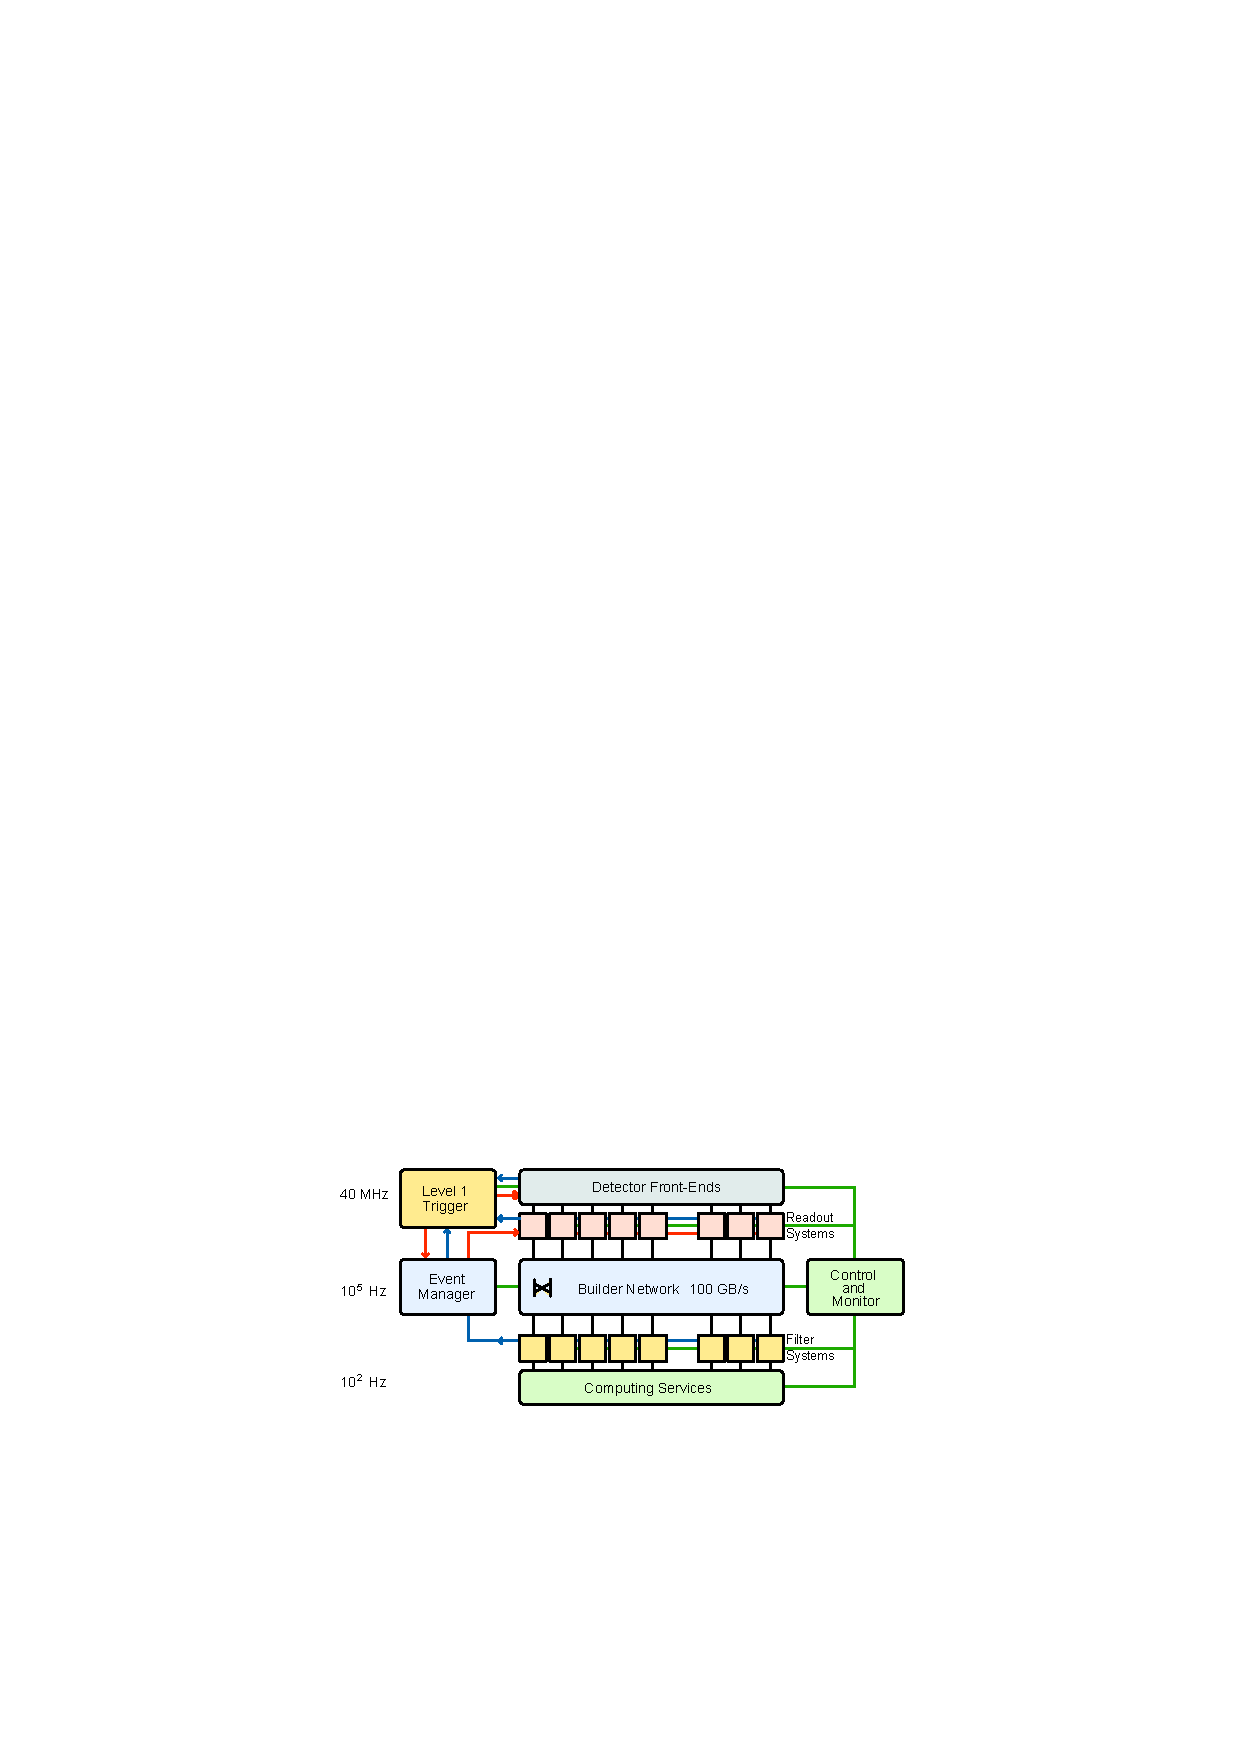
\includegraphics[width=5.5in]{figures/daq.pdf}
\caption{CMS data acquisition system schematic diagram.}
\label{fig:daq}
\end{figure}

\indent In order to verify that the live trigger system is performing as expected and to emulate the trigger system for the production of simulated events, an offline trigger software framework is developed and maintained in parallel with the hardware system. For each calorimeter and muon trigger subsystem, there is a corresponding software emulator that simulates the hardware decisions. The live DQM system used by trigger shifters compares the hardware output to the output of the emulators. In addition to DQM, the trigger software framework is used to calculate the L1T efficiencies, or the efficiency of detection for various reconstructed physics objects. The service work conducted in the process of completing this thesis included contributing to the upgrade of the offline software to be based on calorimeter Layers instead of the regional (RCT) and global trigger (GCT) subsystems of the Run 1 legacy format described above, and the development of automated workflows for trigger DQM. The Run 2 calorimeter trigger system is based on two layers: Layer1, responsible for constructing towers from the energy deposits in ECAL and HCAL modules, and Layer2, which algorithmically builds physics objects from Layer1 towers. A staggered upgrade plan was carried out with the GCT replaced by Layer2 in 2015 (called Stage1) and the RCT to Layer1 in 2016 (called Stage2). During partial upgrades, data formats would be upconverted or downconverted before or after an upgrade stage, where applicable, to keep the entire workflow functioning. 


\chapter{Event reconstruction and simulation}

This chapter overviews the algorithms used to reconstruct the trajectories and identify (ID) types of particles produced in proton-proton collisions in CMS, collectively known as Particle Flow (PF) \cite{CMS:2009nxa}, and how these collisions are simulated.

\section{Particle reconstruction}

The PF algorithms combine information from all of the CMS subdetectors discussed in the previous chapter to reconstruct the particles produced in the collision event. Since many of the particles produced initially in the collision are unstable, decaying before they have time to interact with the subdetectors, PF only reconstructs the stable particles: electrons, muons, photons, and hadrons. The remaining physics objects of interest, jets, missing energy, taus, etc, can be determined from the information provided by the stable PF identified particles. 

\indent The different particles are reconstructed and identified using information from individual subdetectors, or combinations of subdetectors. The direction and momentum of charged particles is measured by the tracker. Electrons are reconstructed using tracks and energy deposits in the ECAL. Muons are reconstructed from a combination of tracker and muon chamber data. Photons are reconstructed from energy deposits in the ECAL. Finally, charged and neutral hadrons are reconstructed from energy deposited primarily in the HCAL, with a contribution from energy deposits in the ECAL. The MET, an observable of particular importance to this analysis, and used to identify DM that does not interact with the detector material, is the modulus of the sum of transverse momenta of all the PF reconstructed particles. 

\indent The basic pieces of information from the subdetectors used by PF are called elements, and consist of charged-particle tracks, muon tracks, and calorimeter clusters. The tracker provides charged-particle track elements. Since the tracker has the best momentum resolution of the subdetectors, it is of critical importance that the tracking efficiency be nearly 100\%, with as low a fake rate as possible, to reduce an excess in reconstructed energy. This goal is accomplished using an iterative algorithm: first, tracks are seeded using very tight criteria, yielding a low efficiency, but negligible fake rate, then track seed criteria are loosened and hits that clearly belong to a track are removed, resulting in increasing efficiency. The ECAL and HCAL subsystems (ECAL barrel, HCAL barrel, HCAL end cap, PS first layer, and PS second layer) provide cluster elements. The calorimeter clustering algorithm measures the energy and direction of neutral particles (i.e. photons and neutral hadrons), differentiates energy deposits from neutral and charged hadrons, reconstructs electrons, and contributes to the reconstruction of charged hadrons. The algorithm is summarized as follows: cluster seeds are identified as energy deposit peaks over a given energy, from which topological clusters are grown by appending adjacent cells, and last, topological clusters seed PF clusters. An example is shown in Figure~\ref{fig:pf1} and Figure~\ref{fig:pf2}, where a simple jet is reconstructed into four clusters, shown as dots. 


\begin{figure}[tbh]
\centering
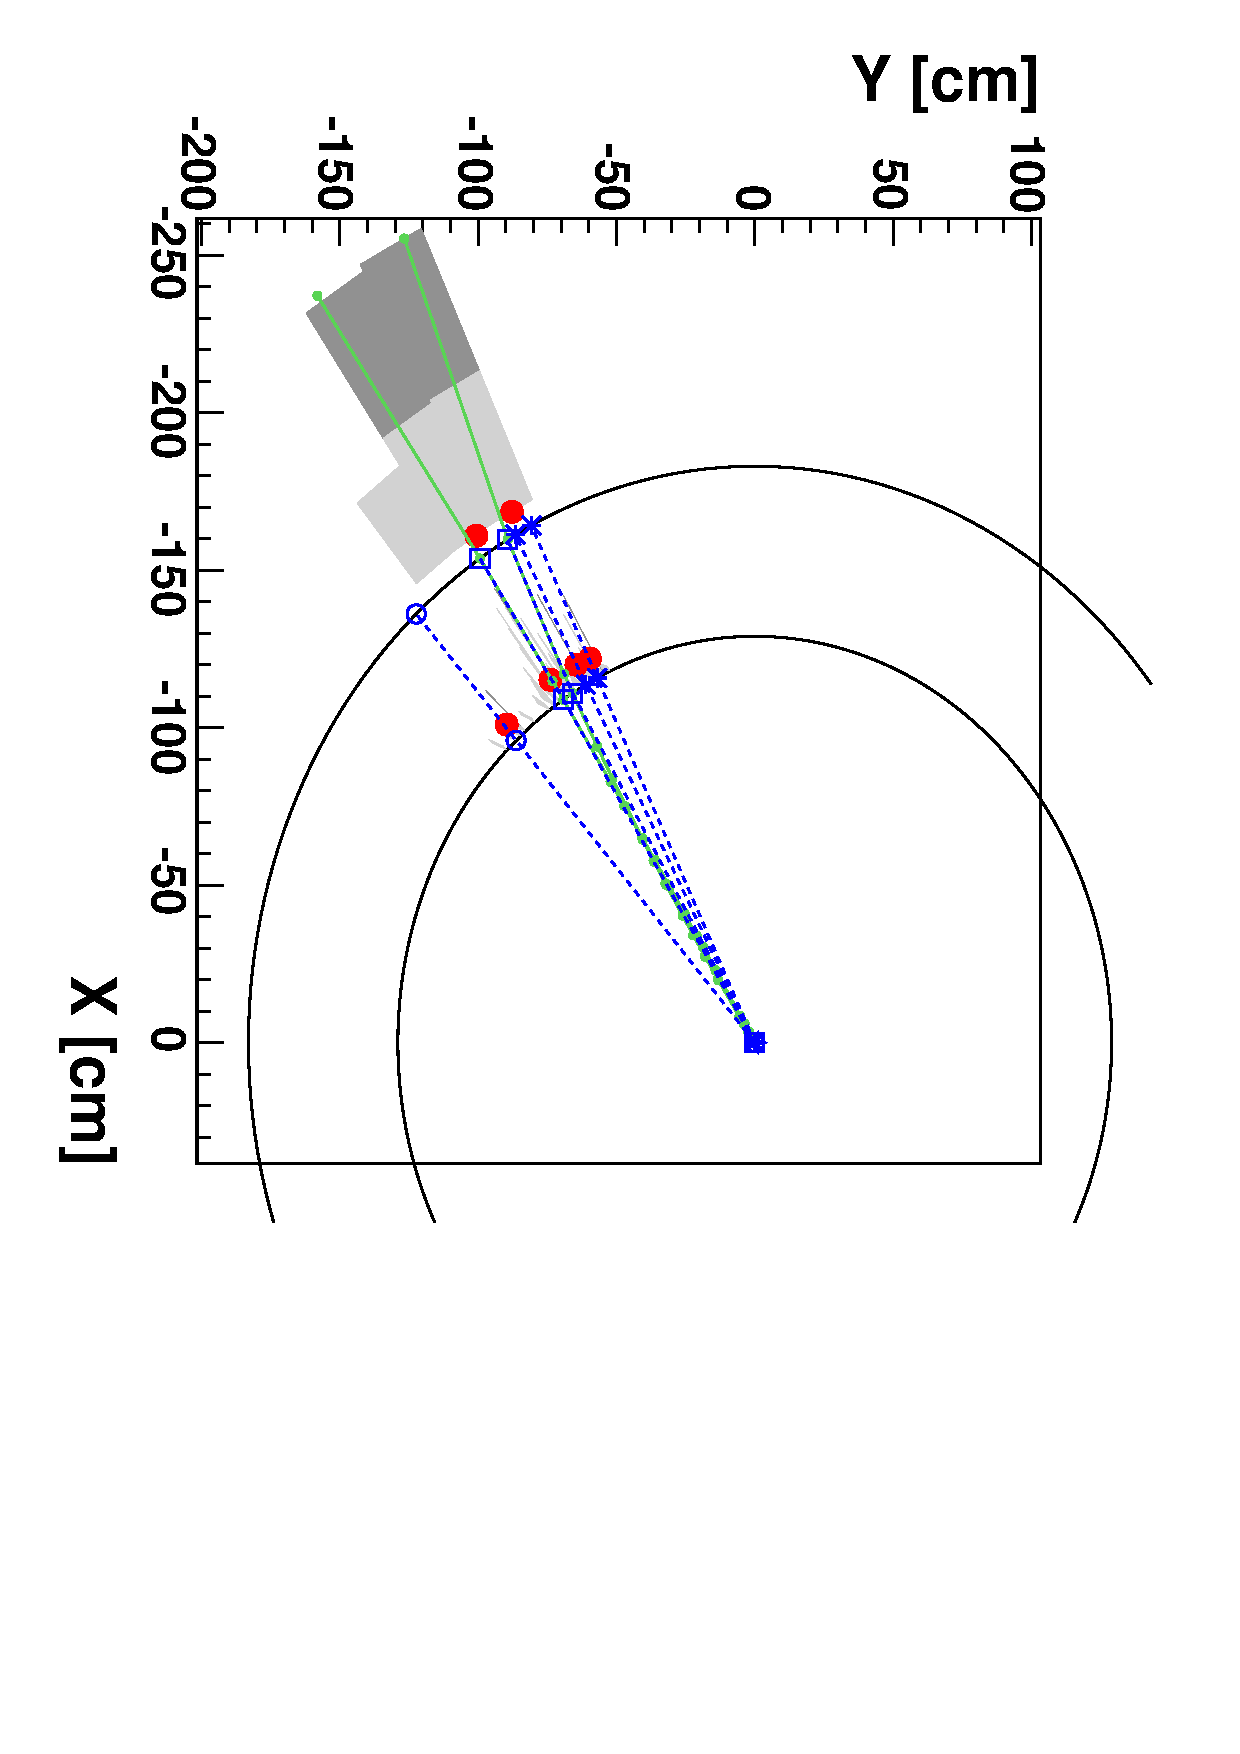
\includegraphics[width=4in]{figures/PFa.pdf}
\caption{Event display of hadronic jet in the $x-y$ plane, with solid arcs at the ECAL and HCAL surfaces. The locations of clusters are given by the solid dots.}
\label{fig:pf1}
\end{figure}

\begin{figure}[tbh]
\begin{subfigure}{0.45\textwidth}
\centering
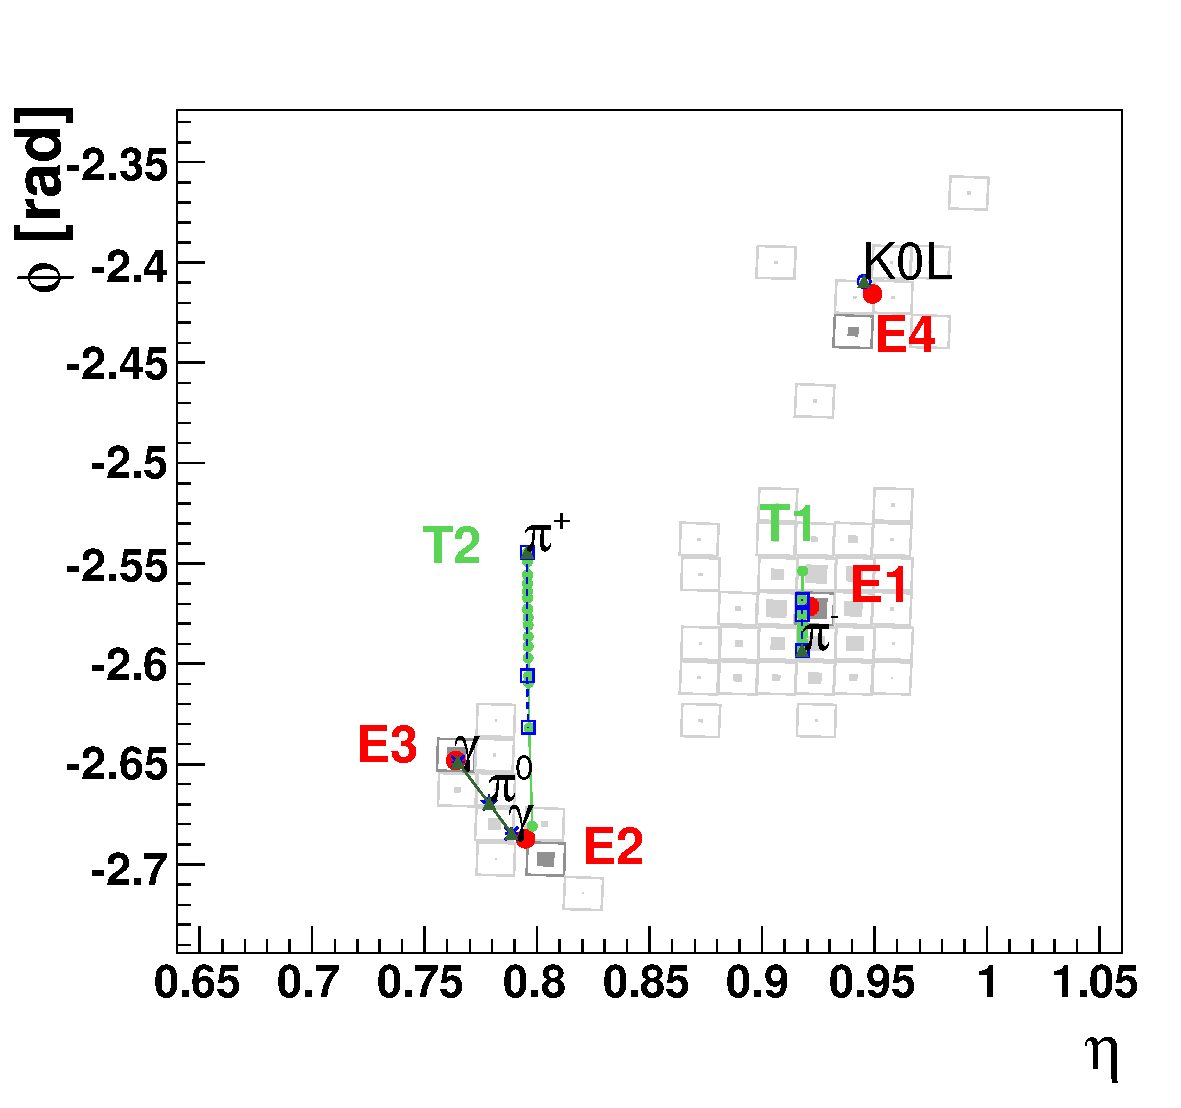
\includegraphics[width=2.8in]{figures/PFb.pdf}
\caption{}
\end{subfigure}
\begin{subfigure}{0.45\textwidth}
\centering
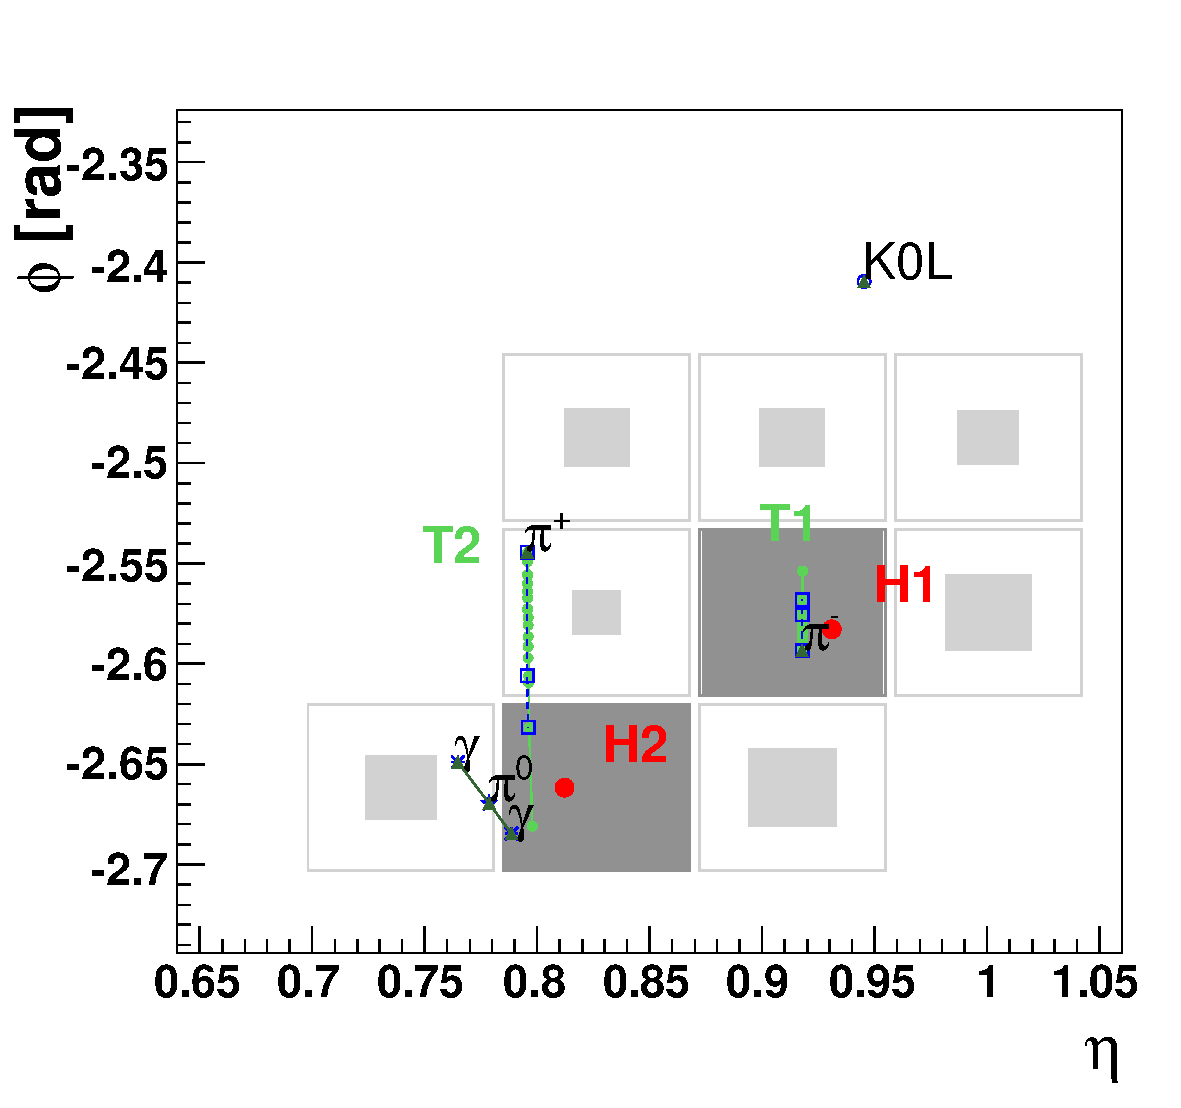
\includegraphics[width=2.8in]{figures/PFc.pdf}
\caption{}
\end{subfigure}
\caption{Event display of hadronic jet in the $\eta-\phi$ plane for the ECAL (a) and HCAL (b). The locations of clusters are given by the solid dots.}
\label{fig:pf2}
\end{figure}

\indent Once the PF elements are determined, they are linked together into blocks, which correspond to the signatures left in the subdetectors of a single particle. Single particles typically leave one to three elements. The linking algorithm determines the quality of the link between all pairwise elements in an event, then forms blocks from the highest quality links, starting from the tracker and proceeding outward through the calorimeters and muon chambers. Once the blocks are formed, PF associates a global event particle with each block. A PF muon is formed from a global muon candidate if its momentum is consistent across all track elements. PF electrons are identified from electron candidates using tracker and ECAL cluster variables, accounting for the bremsstrahlung photons produced when the electron passes through the tracker material. Once the elements associated to PF muons and PF electrons are removed, the remaining elements are analyzed to identify charged hadrons, photons, or neutral hadrons. PF charged hadrons are associated to remaining tracks if the linked clusters are consistent with the measured momenta. If the energy of the linked clusters is much larger than the track momentum, accounting for uncertainties, a PF photon or PF neutral hadron is formed. Any remaning clusters without linked tracks form PF photons or PF neutral hadrons. 

\indent As previously discussed, once the PF particles are identified, additional information about the event can be inferred. A quantity of particular importance to this analysis is the missing transverse energy (MET), defined above. The performance of the PF algorithms' determination of the MET is shown in Figure~\ref{fig:pfmetres} by the resolution of PF measured MET as a function of the true MET to be within $\pm5\%$ above 20 $\GeV$.


\begin{figure}[tbh]
\centering
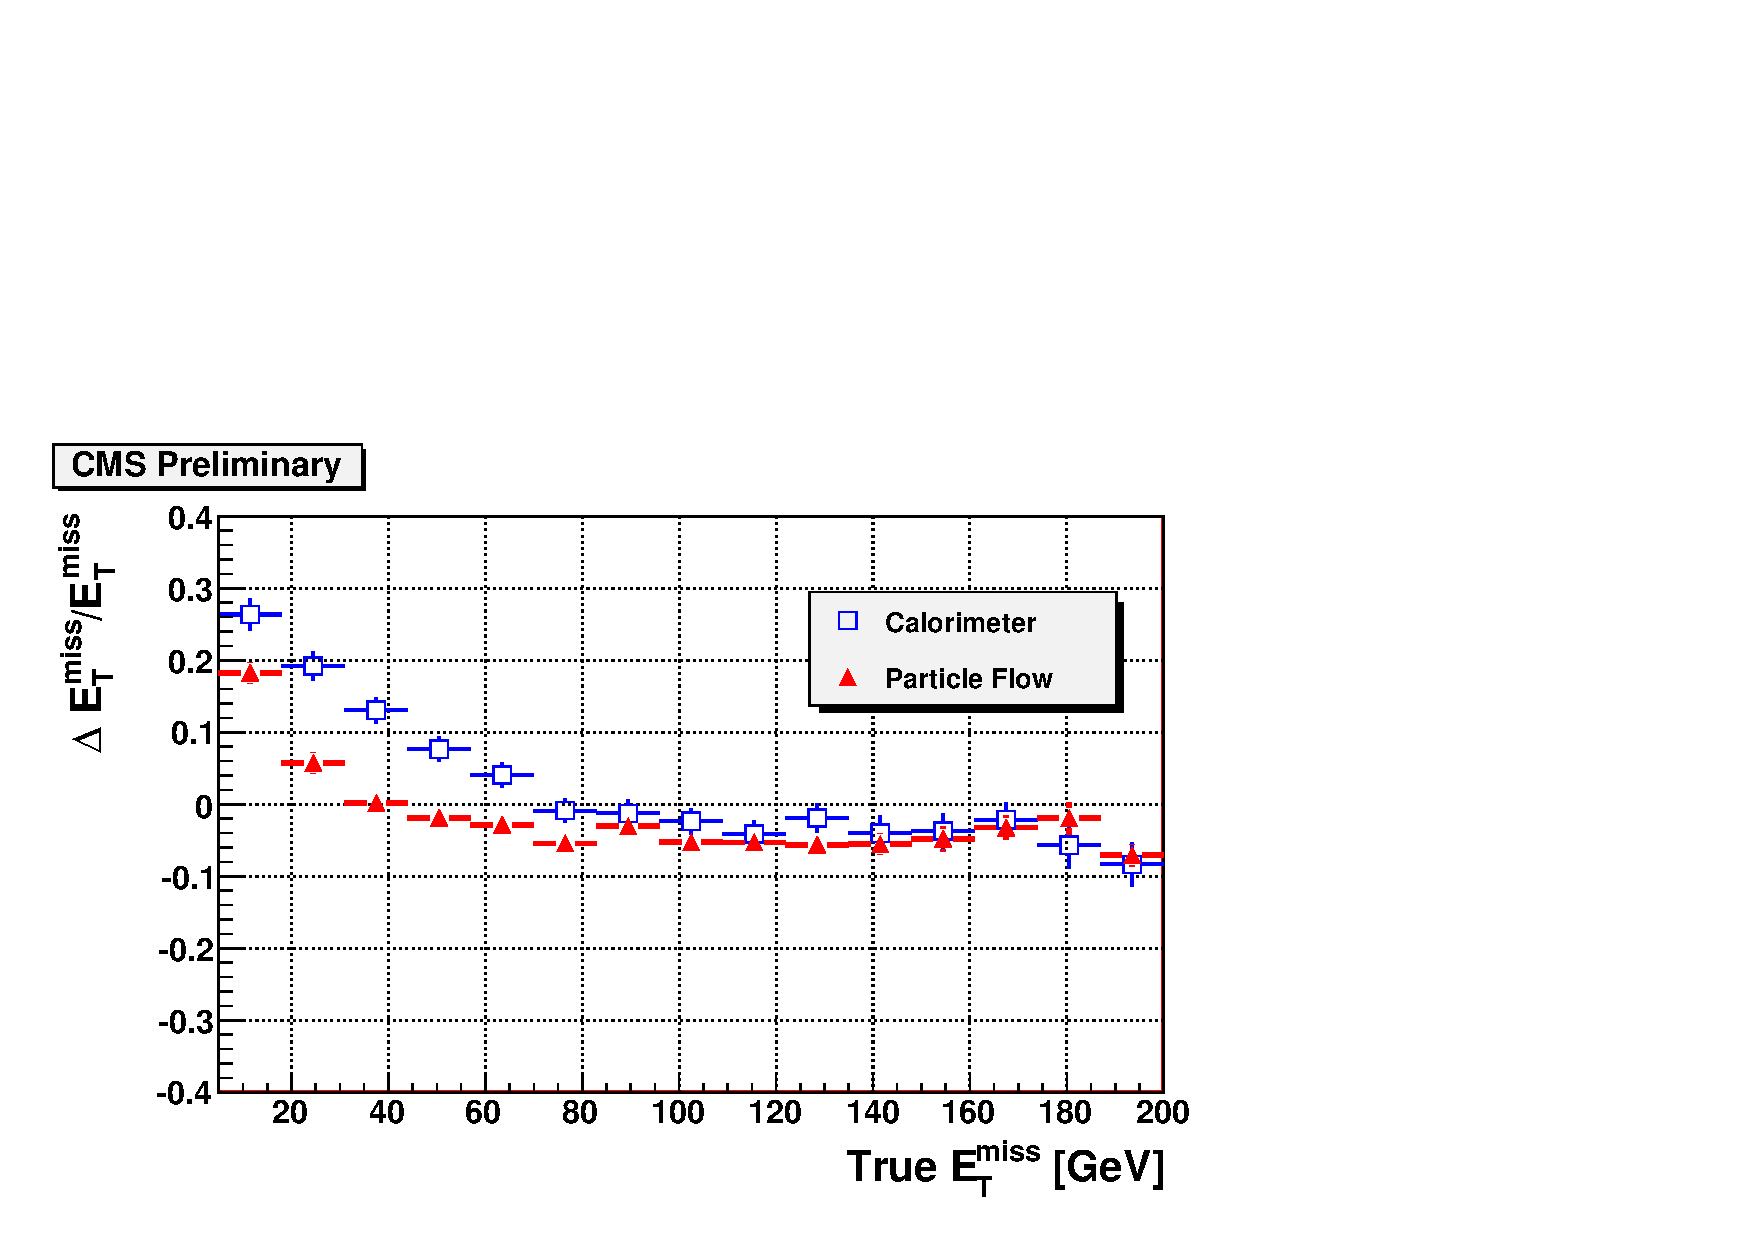
\includegraphics[width=4.5in]{figures/pfmetres.pdf}
\caption{Missing transverse energy reconstruction resolution using the particle flow algorithm.}
\label{fig:pfmetres}
\end{figure}

\section{Monte Carlo event simulation}

The simulation of proton collision events and their detection using Monte Carlo (MC) techniques is useful for several purposes. In addition to using the simulated events to test the detector hardware and software performance without collecting true data, simulations are used to build background models when searching the data for new physics processes. New physics signatures usually appear as excesses in data above a SM background. The background model consists of SM processes which produce the same or similar signature as the new signal being searched for. These processes are modeled either using purely simulated events or a combination of simulated events and data-driven techniques. In either case, it is often necessary to weight the background events by correction scale factors measured using data, which account for shortcomings of the simulations, such as the inability to perform perturbative QCD calculations for low momentum transfer processes. MC event generation can be factored into two parts: (1) modeling the initial particles produced in a collision event and (2) modeling how these initial particles evolve in and interact with the detector.

\indent The first part of MC event generation is modeling the proton-proton collision and the initial particles produced at the primary vertex. Several software packages are used by CMS analysts to generate collision events and calculate the cross sections of the simulated processes, including PYTHIA \cite{1126-6708-2006-05-026}, MADGRAPH \cite{Alwall2011}, BlackHat and Sherpa \cite{Berger:2009ba}, and POWHEG \cite{Alioli:2010ab}. The packages have different implementations, but the underlying principles are the same. The momenta of the proton partons (i.e. quarks and gluons) that interact in the initial scatter are determined probabilistically by random sampling from the parton distribution functions (PDFs), which give the probability that a parton will carry a fraction $x$ of the proton momentum. This is straightforward for processes with two incoming and one outgoing particle ($2 \rightarrow 1$) and two incoming and two outgoing particles ($2 \rightarrow 2$), in which the outcomes are weighted by their relative cross sections and determined probabalistically. However, for radiative processes, such as ISR and FSR of a photon or gluon, which are generally $1 \rightarrow 2$ processes, higher order matrix elements must be calculated or approximated. Once the initial particles are determined, their fragmentation and decays are simulated in a process called hadronization, until the final stable particles are produced. 

\indent The second part of MC event generation is simulating the detector response to the stable particles produced in the first step, including their interaction with the detector material itself, both active elements and structural material. The primary software package used in this step by CMS is GEANT \cite{documents:998155}, in which a complete digital representation of the CMS detector is built. GEANT simulates the passage of each stable particle, step-by-step, outward through the detector, probabilistically determining the interaction that occurs at each step depending on the particle's energy,  material it is in, and the EM field present. The detector is not perfectly efficienct because the acceptance is less than one and the reconstruction efficiency of the individual detector elements is suboptimal, so calibration values must be measured at CMS and fed back in to the simulations, in order to accurately simulate the performance of the detector. Once the final response of the detector is simulated, the resulting MC may be weighted by scale factors measured using real data, in order to correct for mismodeling of the detector.

\section{Datasets}

\subsection{Data}

\subsubsection{Triggers and Datasets}
\label{sec:trigpaths}

This analysis uses a data sample recorded by the CMS experiment during 2016, corresponding to $\usedLumi$ of data. 
The datasets are listed in Table~\ref{tab:datasets_data}, along with their integrated luminosities.  
The analysis relies on five different primary datasets (PDs) $-$ 
DoubleEG, DoubleMuon, MuEG, SingleElectron, and SingleMuon $-$
each of which combines a certain collection of HLT paths. 
To avoid duplicate events from different primary datasets, events are taken:
\begin{itemize}
\item from DoubleEG if they pass the diEle or triEle triggers,
\item from DoubleMuon if they pass the diMuon or triMuon triggers and fail the diEle and triEle triggers,
\item from MuEG if they pass the MuEle or MuDiEle or DiMuEle triggers and fail the diEle, triEle, diMuon and triMuon triggers,
\item from SingleElectron if they pass the singleElectron trigger and fail all the above triggers. 
\item from SingleMuon if they pass the singleMuon trigger and fail all the above triggers. 
\end{itemize} 

The HLT paths used for 2016 collision data are listed in Table~\ref{tab:triggerPaths}, 
together with their L1 seeds, prescale values and the associated primary datasets.

%The JSON files are the following:
%\begin{itemize}
%\item Cert\_13TeV\_16Dec2015ReReco\_Collisions15\_50ns\_JSON.txt (for 50 ns data),
%\item Cert\_13TeV\_16Dec2015ReReco\_Collisions15\_25ns\_JSON\_Silver.txt (for 25 ns data).
%\end{itemize} 

\begin{table}[h]
\tiny
    \centering
    \begin{tabular}{|l|l|l|} 
\hline %----------------------------------------------------------------------------------------
\hline %---------------------------------------------------------------------------------------- 
Run-range & Dataset & Integrated luminosity \\
\hline %----------------------------------------------------------------------------------------
\hline %---------------------------------------------------------------------------------------- 
\multirow{5}{*}{273150-275376} & /DoubleMuon/Run2016B-23Sep2016-v3/AOD &  \multirow{5}{*}{$5.892\ \text{fb}^{-1}$} \\ 
& /DoubleEG/Run2016B-23Sep2016-v3/AOD &  \\ 
& /MuonEG/Run2016B-23Sep2016-v3/AOD &  \\ 
& /SingleElectron/Run2016B-23Sep2016-v3/AOD &  \\ 
& /SingleMuon/Run2016B-23Sep2016-v3/AOD &  \\ 
\hline
\multirow{5}{*}{275656-276283} & /DoubleMuon/Run2016C-23Sep2016-v1/AOD &  \multirow{5}{*}{$2.646\ \text{fb}^{-1}$}  \\ 
& /DoubleEG/Run2016C-23Sep2016-v1/AOD &  \\ 
& /MuonEG/Run2016C-23Sep2016-v1/AOD &  \\ 
& /SingleElectron/Run2016C-23Sep2016-v1/AOD &  \\ 
& /SingleMuon/Run2016C-23Sep2016-v1/AOD &  \\ 
\hline
\multirow{5}{*}{276315-276811} & /DoubleMuon/Run2016D-23Sep2016-v1/AOD &  \multirow{5}{*}{$4.353\ \text{fb}^{-1}$} \\ 
& /DoubleEG/Run2016D-23Sep2016-v1/AOD &  \\ 
& /MuonEG/Run2016D-23Sep2016-v1/AOD &  \\ 
& /SingleElectron/Run2016D-23Sep2016-v1/AOD &  \\ 
& /SingleMuon/Run2016D-23Sep2016-v1/AOD &  \\ 
\hline
\multirow{5}{*}{276831-277420} & /DoubleMuon/Run2016E-23Sep2016-v1/AOD &  \multirow{5}{*}{$4.117\ \text{fb}^{-1}$} \\ 
& /DoubleEG/Run2016E-23Sep2016-v1/AOD &  \\ 
& /MuonEG/Run2016E-23Sep2016-v1/AOD &  \\ 
& /SingleElectron/Run2016E-23Sep2016-v1/AOD &  \\ 
& /SingleMuon/Run2016E-23Sep2016-v1/AOD &  \\ 
\hline
\multirow{5}{*}{277932-278808} & /DoubleMuon/Run2016F-23Sep2016-v1/AOD &  \multirow{5}{*}{$3.186\ \text{fb}^{-1}$} \\ 
& /DoubleEG/Run2016F-23Sep2016-v1/AOD &  \\ 
& /MuonEG/Run2016F-23Sep2016-v1/AOD &  \\ 
& /SingleElectron/Run2016F-23Sep2016-v1/AOD &  \\ 
& /SingleMuon/Run2016F-23Sep2016-v1/AOD &  \\ 
\hline
\multirow{5}{*}{278820-280385} & /DoubleMuon/Run2016G-23Sep2016-v1/AOD &  \multirow{5}{*}{$7.721\ \text{fb}^{-1}$} \\ 
& /DoubleEG/Run2016G-23Sep2016-v1/AOD &  \\ 
& /MuonEG/Run2016G-23Sep2016-v1/AOD &  \\ 
& /SingleElectron/Run2016G-23Sep2016-v1/AOD &  \\ 
& /SingleMuon/Run2016G-23Sep2016-v1/AOD &  \\ 
\hline
\multirow{15}{*}{281207-284068} & /DoubleMuon/Run2016H-PromptReco-v1/AOD &  \multirow{15}{*}{$8.857\ \text{fb}^{-1}$} \\ 
& /DoubleEG/Run2016H-PromptReco-v1/AOD &  \\ 
& /MuonEG/Run2016H-PromptReco-v1/AOD &  \\ 
& /SingleElectron/Run2016H-PromptReco-v1/AOD &  \\ 
& /SingleMuon/Run2016H-PromptReco-v1/AOD &  \\ 
& /DoubleMuon/Run2016H-PromptReco-v2/AOD &  \\ 
& /DoubleEG/Run2016H-PromptReco-v2/AOD &  \\ 
& /MuonEG/Run2016H-PromptReco-v2/AOD &  \\ 
& /SingleElectron/Run2016H-PromptReco-v2/AOD &  \\ 
& /SingleMuon/Run2016H-PromptReco-v2/AOD &  \\ 
& /DoubleMuon/Run2016H-PromptReco-v3/AOD &  \\ 
& /DoubleEG/Run2016H-PromptReco-v3/AOD &  \\ 
& /MuonEG/Run2016H-PromptReco-v3/AOD &  \\ 
& /SingleElectron/Run2016H-PromptReco-v3/AOD &  \\ 
& /SingleMuon/Run2016H-PromptReco-v3/AOD &  \\ 
\hline %----------------------------------------------------------------------------------------
\hline %----------------------------------------------------------------------------------------
     \end{tabular}
%\small
    \caption{Run 2 datasets used in the $H\rightarrow ZZ$ analysis. The first column specifies the range of run ids, indices counting up from the first CMS run, for each dataset. The middle column gives the CMS database file path where the data files are stored. The third column gives the total integrated luminosities for each collection of runs.}
    \label{tab:datasets_data}
\end{table}


\begin{table}[h]
\tiny
    \centering
    \begin{tabular}{|l|l|c|l|} 
\hline %--------------------------------------------------------------------------------------------------------------------------
HLT path                      				       & L1 seed                          & prescale  & primary dataset \\
\hline %--------------------------------------------------------------------------------------------------------------------------
\verb| HLT_Ele17_Ele12_CaloIdL_TrackIdL_IsoVL_DZ       | & \verb| L1_DoubleEG_15_10    |  & 1 & DoubleEG \\
\verb| HLT_Ele23_Ele12_CaloIdL_TrackIdL_IsoVL_DZ       | & \verb| L1_DoubleEG_22_10    |  & 1 & DoubleEG \\
\verb| HLT_DoubleEle33_CaloIdL_GsfTrkIdVL              | & \verb| (Multiple)           |  & 1 & DoubleEG \\
\verb| HLT_Ele16_Ele12_Ele8_CaloIdL_TrackIdL           | & \verb| L1_TripleEG_14_10_8  |  & 1 & DoubleEG \\
\verb| HLT_Mu17_TrkIsoVVL_Mu8_TrkIsoVVL                | & \verb| L1_DoubleMu_11_4     |  & 1 & DoubleMuon \\
\verb| HLT_Mu17_TrkIsoVVL_TkMu8_TrkIsoVVL              | & \verb| L1_DoubleMu_11_4     |  & 1 & DoubleMuon \\
\verb| HLT_TripleMu_12_10_5                            | & \verb| L1_TripleMu_5_5_3    |  & 1 & DoubleMuon \\
\verb| HLT_Mu8_TrkIsoVVL_Ele17_CaloIdL_TrackIdL_IsoVL  | & \verb| L1_Mu5_EG15          |  & 1 & MuonEG \\
\verb| HLT_Mu8_TrkIsoVVL_Ele23_CaloIdL_TrackIdL_IsoVL  | & \verb| L1_Mu5_EG20          |  & 1 & MuonEG \\
\verb| HLT_Mu17_TrkIsoVVL_Ele12_CaloIdL_TrackIdL_IsoVL | & \verb| L1_Mu12_EG10         |  & 1 & MuonEG \\
\verb| HLT_Mu23_TrkIsoVVL_Ele12_CaloIdL_TrackIdL_IsoVL | & \verb| L1_Mu20_EG10         |  & 1 & MuonEG \\
\verb| HLT_Mu23_TrkIsoVVL_Ele8_CaloIdL_TrackIdL_IsoVL  | & \verb| L1_SingleMu*         |  & 1 & MuonEG \\
\verb| HLT_Mu8_DiEle12_CaloIdL_TrackIdL                | & \verb| L1_Mu6_DoubleEG10    |  & 1 & MuonEG \\
\verb| HLT_DiMu9_Ele9_CaloIdL_TrackIdL                 | & \verb| L1_DoubleMu7_EG7     |  & 1 & MuonEG \\
\verb| HLT_Ele25_eta2p1_WPTight                        | & \verb| L1_SingleEG*         |  & 1 & SingleElectron \\
\verb| HLT_Ele27_WPTight                               | & \verb| L1_SingleEG*         |  & 1 & SingleElectron \\
\verb| HLT_Ele27_eta2p1_WPLoose_Gsf                    | & \verb| L1_SingleEG*         |  & 1 & SingleElectron \\
\verb| HLT_IsoMu20 OR HLT_IsoTkMu20                    | & \verb| L1_SingleMu*         |  & 1 & SingleMuon \\
\verb| HLT_IsoMu22 OR HLT_IsoTkMu22                    | & \verb| L1_SingleMu*         |  & 1 & SingleMuon \\
\hline %--------------------------------------------------------------------------------------------------------------------------
    \end{tabular}
%\small
    \caption{Trigger paths used in 2016 collision data.}
    \label{tab:triggerPaths}
\end{table}


\subsubsection{Trigger Efficiency}

The efficiency for data events to pass the combination of triggers with respect to the offline reconstruction and selection is measured
by considering four-lepton events triggered by single lepton triggers. One of the four reconstructed leptons, called the "tag," is geometrically matched 
to a trigger object passing the final filter of one of the single muon or single electron triggers. The other three leptons are 
used as ``probes.'' In each four-lepton event, there are up to four possible tag-probe combinations, and all possible combinations are counted in the
denominator of the efficiency. For each of the three probe leptons, all matching trigger filter objects are collected. Then, the matched trigger filter
objects of the three probe leptons are combined in attempt to reconstruct any of the triggers used in the analysis. If any of the analysis triggers
can be formed using the probe leptons, the set of probes is also counted in the numerator of the efficiency.

This method does not have a perfect closure in MC events due to the fact that the presence of a fourth lepton increases the trigger efficiency,
and this effect is not accounted for. Also, in the  $2e2\mu$ final state, the three probe leptons cannot be combined to form all possible triggers which 
can collect events with two electrons and two muons (e.g. if the tag lepton is an electron, the three remaining leptons cannot pass a double electron
trigger). Therefore, the method is also exercised on MC, and the difference between data and MC is used to determine the reliability of the simulation.
 The efficiency plotted as a function of the minimum transverse momentum ($p_{\rm{T}}$) of the three probe leptons in data and MC using this method can be seen in 
Figure~\ref{fig:TrigEff}. The MC efficiency describes the data within the statistical uncertainties well.

%=======
\begin{figure}[!htb]
\vspace*{0.3cm}
\begin{center}
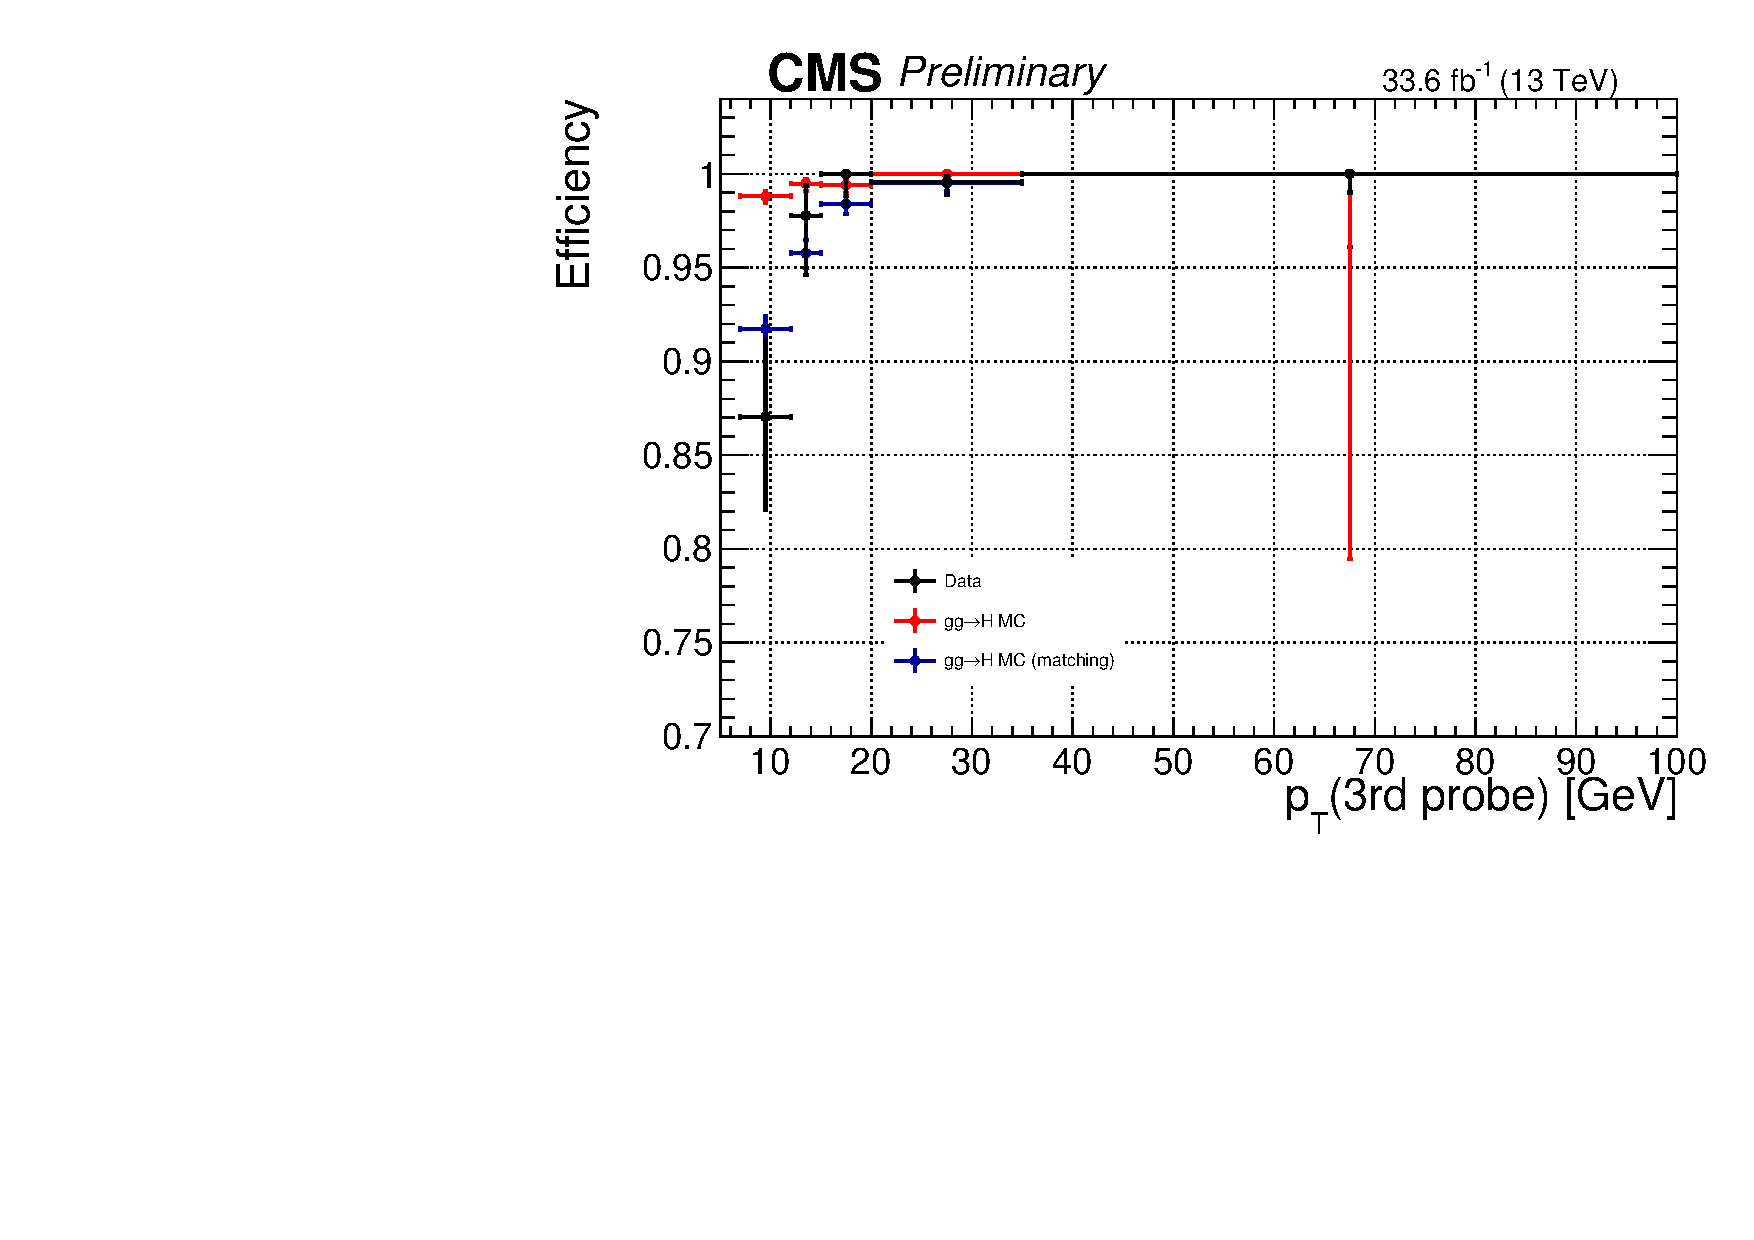
\includegraphics[width=0.45\textwidth]{Figures/Trigger/Histo_TrigEff_ptMin_4e.pdf} 
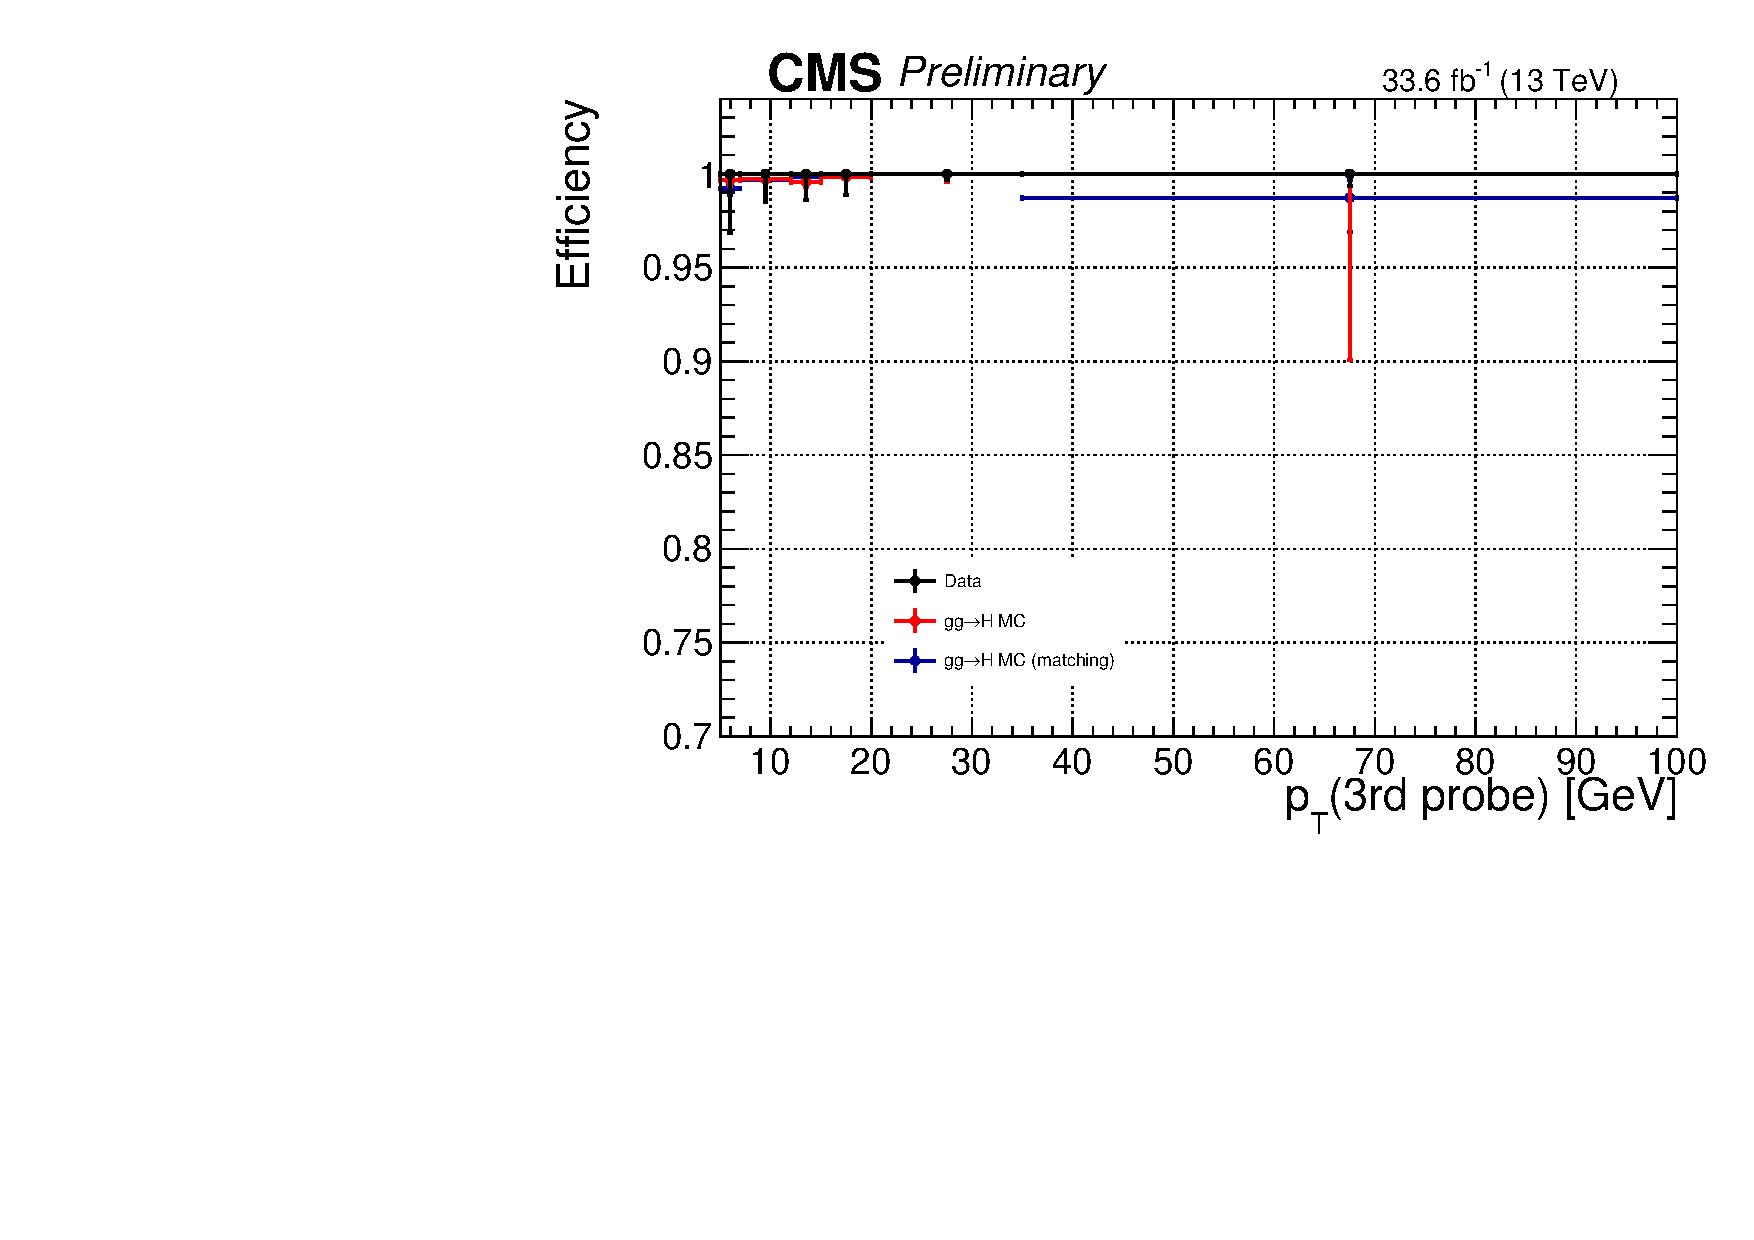
\includegraphics[width=0.45\textwidth]{Figures/Trigger/Histo_TrigEff_ptMin_4mu.pdf} \\
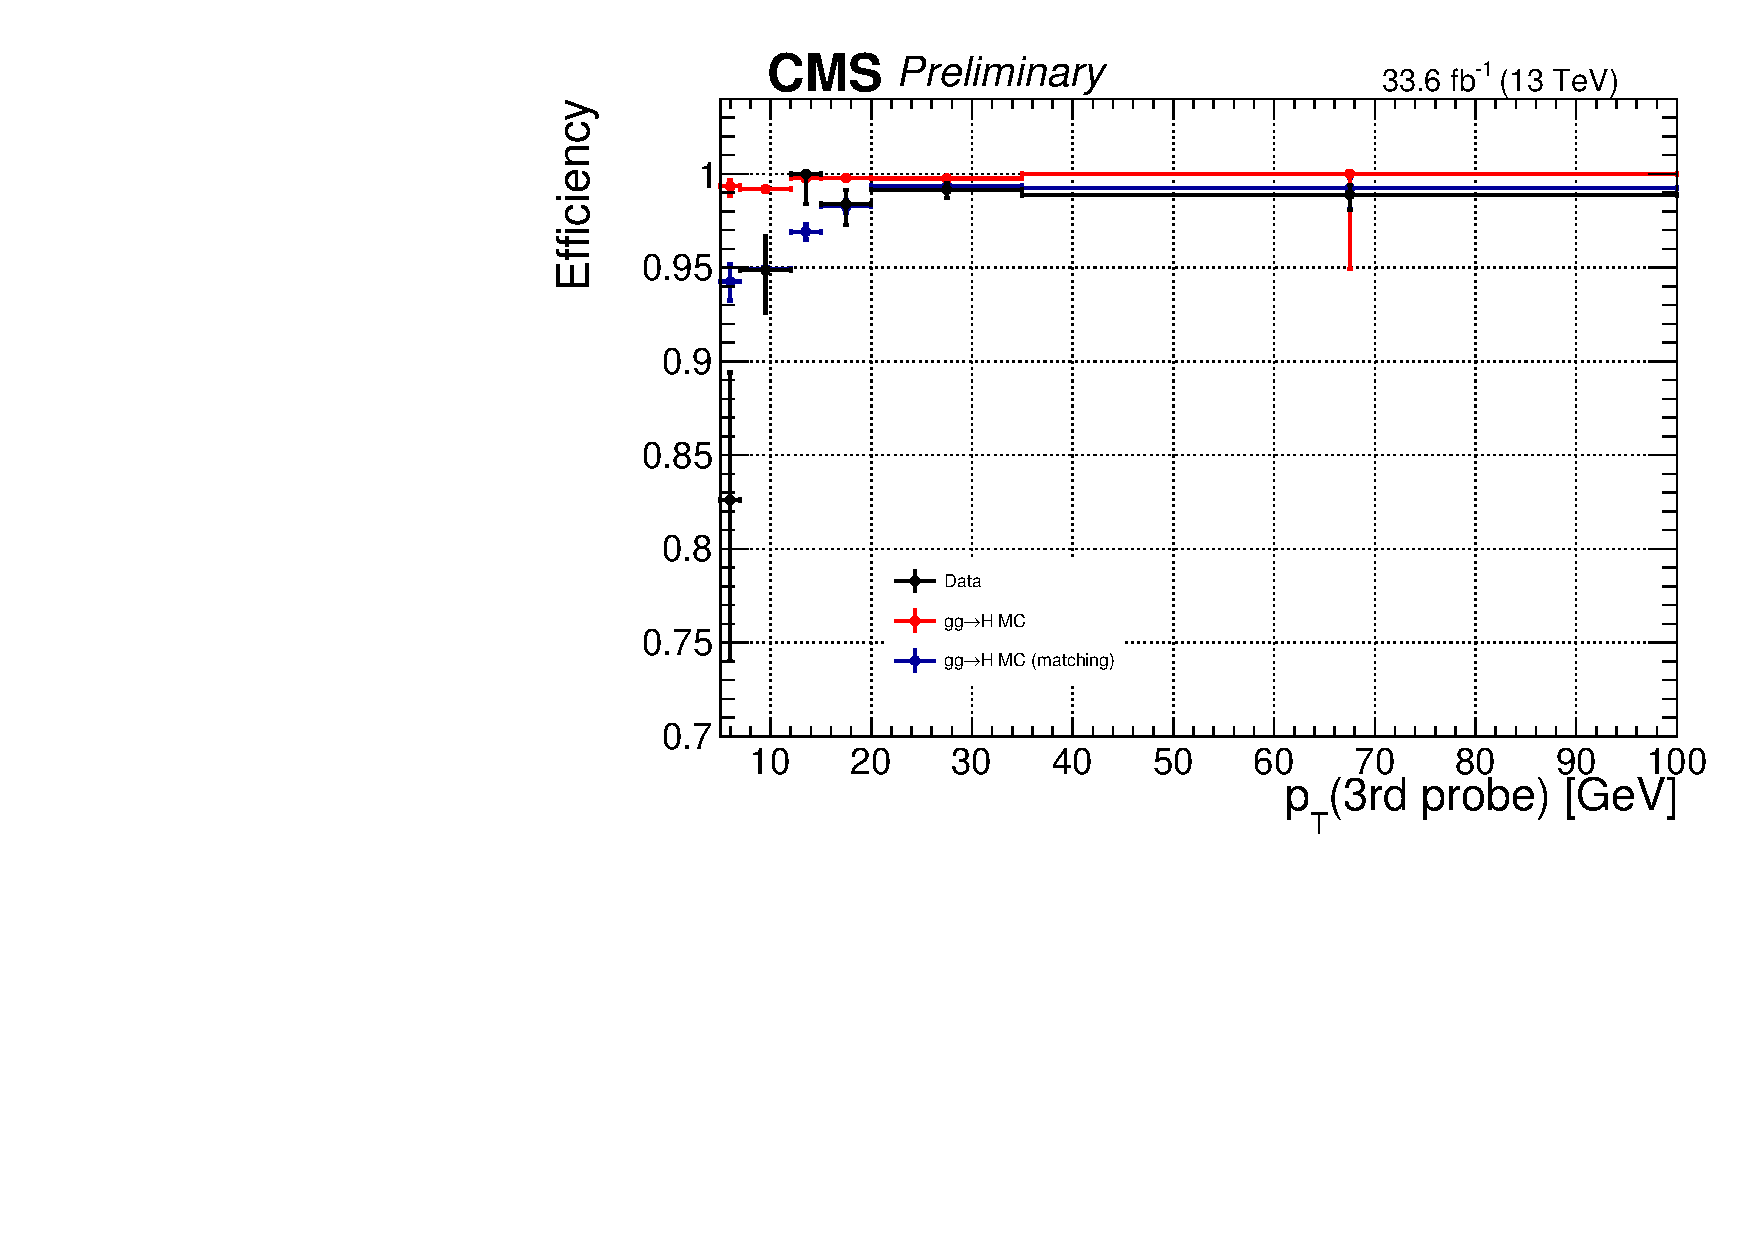
\includegraphics[width=0.45\textwidth]{Figures/Trigger/Histo_TrigEff_ptMin_2e2mu.pdf} 
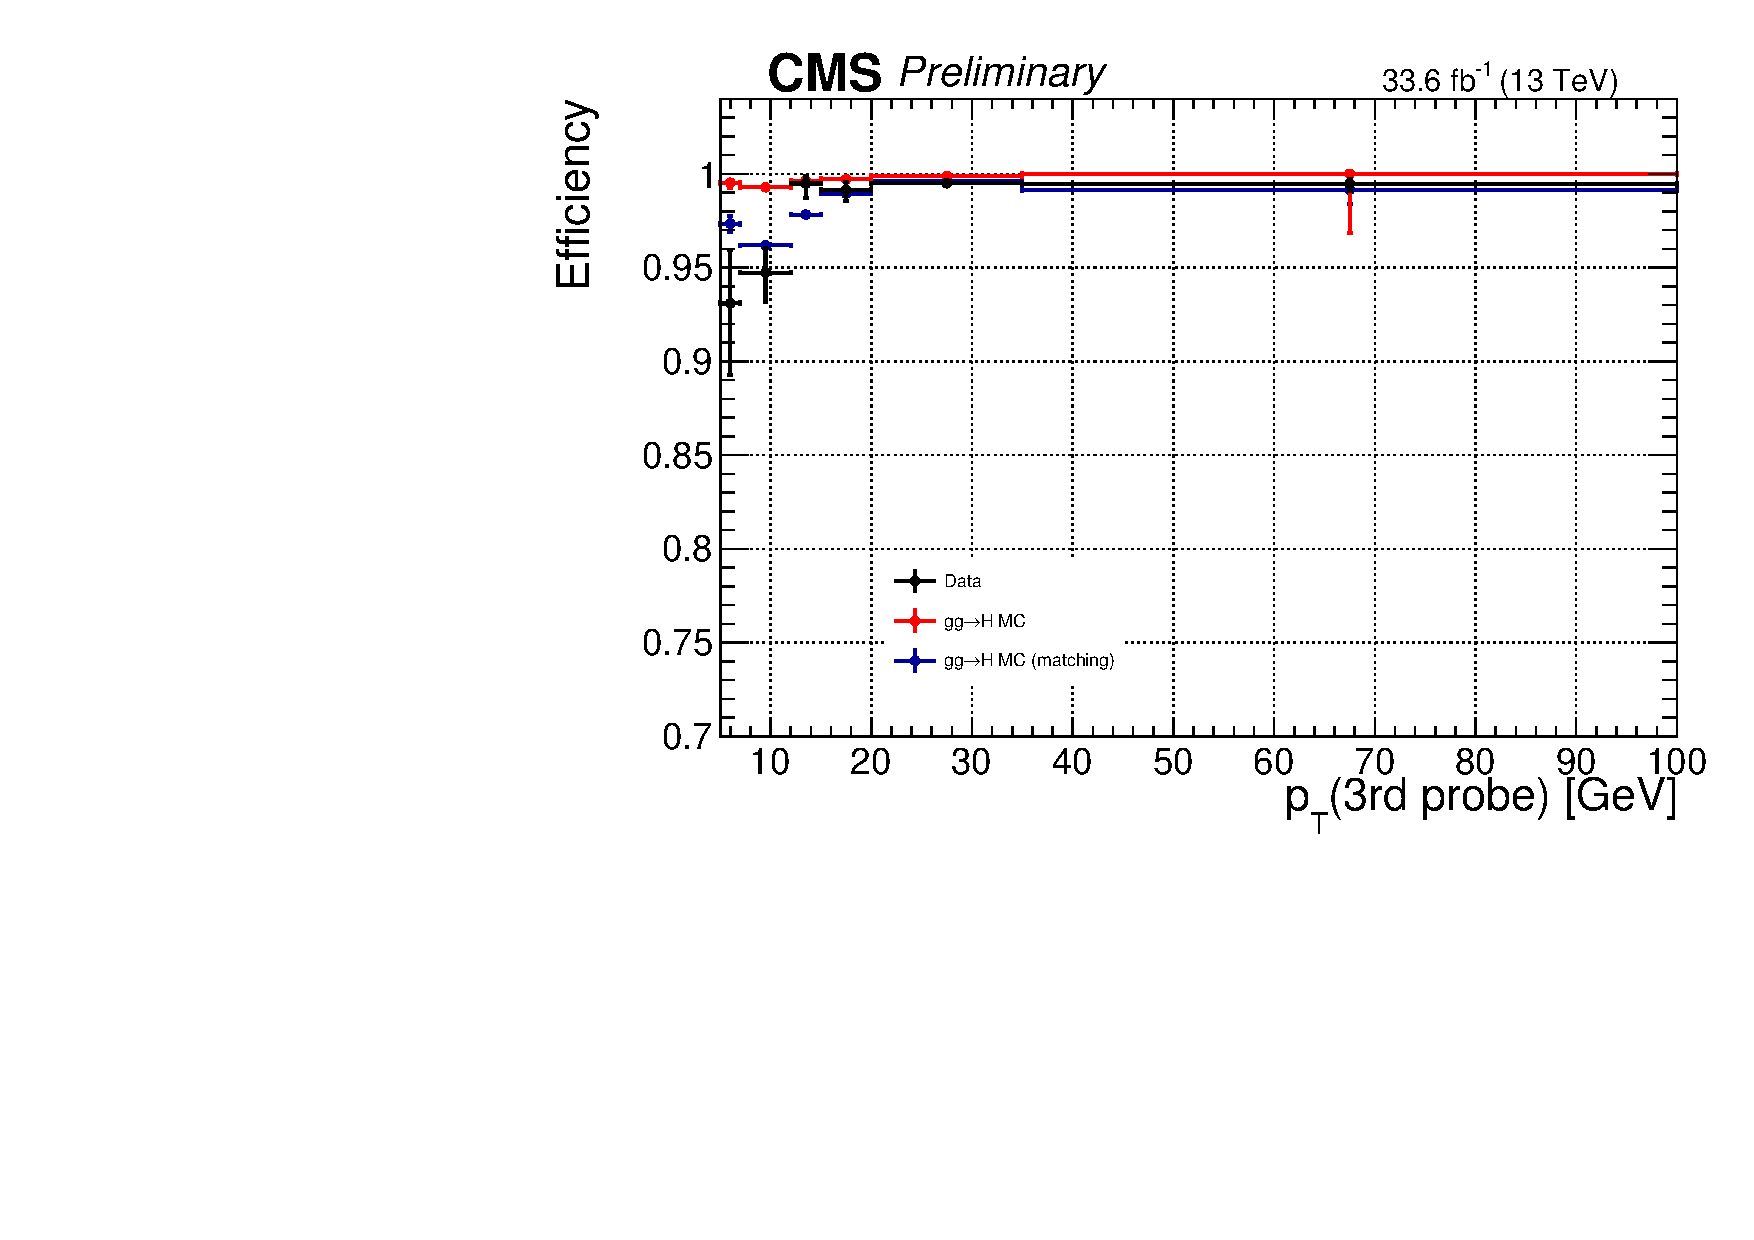
\includegraphics[width=0.45\textwidth]{Figures/Trigger/Histo_TrigEff_ptMin_4l.pdf} \\
\caption{Trigger efficiency measured in data using $4\ell$ events collected by single lepton triggers for the $4e$ (top left), $4\mu$ (top right), $2e2\mu$ (bottom left) and $4\ell$ (bottom right) final states. 
\label{fig:TrigEff}}
\end{center}
\end{figure}
%=======

A summary of the trigger efficiencies in MC truth, MC, and data using the tag and probe method, is shown in Table~\ref{tab:TrigEff}. The trigger
efficiency in simulation is found to be $>99\%$ in each final state.

\begin{table}[h]
    \centering
    \begin{tabular}{|c|c|c|c|c|} 
\hline %----------------------------------------------------------------
Final State  & $\ggH$ MC & $\ggH$ MC (matching)  & Data (matching)   \\
\hline %----------------------------------------------------------------
$4e$  & 0.991$^{+.002}_{-0.002}$ & 0.948$^{+.004}_{-0.004}$ & 0.982$^{+.005}_{-0.007}$ \\
$4\mu$  & 0.997$^{+.001}_{-0.001}$ & 0.997$^{+.001}_{-0.001}$ & 1.000$^{+.000}_{-0.001}$ \\
$2e2\mu$  & 0.995$^{+.001}_{-0.001}$ & 0.964$^{+.002}_{-0.002}$ & 0.983$^{+.003}_{-0.004}$ \\
\hline %----------------------------------------------------------------
    \end{tabular}
    \caption{Trigger efficiencies measured using $4\ell$ events.}
    \label{tab:TrigEff}
\end{table}

\subsection{Simulation}

\subsubsection{Signal Samples}

The signal samples used are centrally produced for the benchmarks defined in Section~\ref{sec:sigbench} and are summarized in Table~\ref{tab:sig}.

\begin{table}
\resizebox{\textwidth}{!}{%
\begin{tabular}{| l | l |}
\hline
Dataset & Parameters\\
\hline
/ZprimeToA0hToA0chichihZZTo4l\_2HDM\_MZp-*\_MA0-300\_13TeV-madgraph-pythia8/[1] & $m_{A^0} = $ 300 $\GeV$ \\
/ZprimeToA0hToA0chichihZZTo4l\_2HDM\_MZp-*\_MA0-*\_13TeV-madgraph/[2] & $m_{A^0} \neq $ 300 $\GeV$ \\
/MonoHZZ4l\_ZpBaryonic\_MZp-*\_MChi-*\_13TeV-madgraph/[3] & \\
\hline
$[1]$ RunIISpring16DR80-premix\_withHLT\_80X\_mcRun2\_asymptotic\_v14-v1/AODSIM & \\
$[2]$ RunIISpring16reHLT80-PUSpring16RAWAODSIM\_reHLT\_80X\_mcRun2\_asymptotic\_v14-v1/AODSIM & \\
$[3]$ RunIISpring16DR80-premix\_withHLT\_80X\_mcRun2\_asymptotic\_v14-v1/AODSIM & \\
\hline
\end{tabular}}
\caption{Benchmark signal samples analyzed.}\label{tab:sig}
\end{table}

\subsubsection{Background Samples}

Descriptions of the SM Higgs boson production are obtained using the 
{\sc powheg V2}~\cite{Alioli:2008gx,Nason:2004rx,Frixione:2007vw} generator for the five main production modes: 
gluon fusion ($\ggH$) including quark mass effects~\cite{Bagnaschi:2011tu}, vector boson fusion 
(VBF)~\cite{Nason:2009ai}, and associated production ($WH$, $\cPZ H$ and $\ttbar H$ \cite{Hartanto:2015uka}). 
In the case of $WH$ and $\cPZ H$, the {\sc MiNLO HVJ} extension of {\sc powheg} is used~\cite{Luisoni:2013kna}. 
The description of the decay of the Higgs boson to four leptons is obtained using the {\sc JHUgen} 
generator~\cite{Gao:2010qx}. In the case of $WH$, $\cPZ H$ and $\ttbar H$, the Higgs boson is allowed
to decay to H$\to \cPZ \cPZ \to 2\ell2 X$, such that four-lepton events where two leptons originate from 
the decay of associated $\cPZ$, $W$ bosons or top quarks are also taken into account in the simulation. 
Showering of parton-level events is done using {\sc pythia8.209}, and in all cases, matching is performed by 
allowing QCD emissions at all energies in the shower and vetoing them afterwards according to the 
{\sc powheg} internal scale. All samples are generated with the NNPDF 3.0 next-to-leading order (NLO) PDFs~\cite{Ball:2014uwa}. The list of Higgs signal samples and their cross sections are shown in 
Table~\ref{tab:SignalSamples}.

\begin{table}
\begin{scriptsize}
    \centering
\resizebox{\textwidth}{!}{%
    \begin{tabular}{|l|l|r|}
   \hline
 Process & Dataset & $\sigma\times BR (\times\epsilon_{\text{filter}})$ \\ \hline
 $\rm{gg}\to\rm{H}\to\cPZ\cPZ \to 4\ell$ & /GluGluHToZZTo4L\_M125\_13TeV\_powheg2\_JHUgenV6\_pythia8 & $12.18~\rm{fb}$ \\ % & $12.12~\rm{fb}$ \\
 $\rm{qq}\to\rm{Hqq}\to\cPZ\cPZ\rm{qq}\to4\ell qq$ & /VBF\_HToZZTo4L\_M125\_13TeV\_powheg2\_JHUgenV6\_pythia8 & $1.044~\rm{fb}$ \\ % $1.034~\rm{fb}$ \\
 $\rm{q\bar{q}}\to\rm{W^{+}H}\to\rm{W^{+}}\cPZ\cPZ\to4\ell+\rm{X}$ & /WplusH\_HToZZTo4L\_M125\_13TeV\_powheg2-minlo-HWJ\_JHUgenV6\_pythia8 & $0.232~\rm{fb}$ \\ % $0.2339~\rm{fb}$ \\
 $\rm{q\bar{q}}\to\rm{W^{-}H}\to\rm{W^{-}}\cPZ\cPZ\to4\ell+\rm{X}$ & /WminusH\_HToZZTo4L\_M125\_13TeV\_powheg2-minlo-HWJ\_JHUgenV6\_pythia8 & $0.147~\rm{fb}$ \\ % $0.1471~\rm{fb}$ \\
 $\rm{q\bar{q}}\to\cPZ \rm{H}\to\cPZ\cPZ\cPZ\to4\ell+\rm{X}$ & /ZH\_HToZZ\_4LFilter\_M125\_13TeV\_powheg2-minlo-HZJ\_JHUgenV6\_pythia8 & $0.668~\rm{fb}$ \\ % $0.652~\rm{fb}$ \\
 $\rm{gg}\to\rm{ttH} \to\rm{tt}\cPZ\cPZ\to4\ell+\rm{X}$ & /ttH\_HToZZ\_4LFilter\_M125\_13TeV\_powheg\_JHUgen\_pythia8 & $0.393~\rm{fb}$ \\ % $0.337~\rm{fb}$ \\ 
 \hline
 %\multicolumn{3}{l}{[1] RunIISummer16MiniAODv2-PUMoriond17\_80X\_mcRun2\_asymptotic\_2016\_TrancheIV\_v6-v1} \\
 \end{tabular}}
 \caption{Higgs signal samples and production cross sections times branching fractions to four leptons times filter efficiencies.}
  \label{tab:SignalSamples}
\end{scriptsize}
\end{table}

Production of $ZZ$ via quark-antiquark annihilation is generated at NLO using {\sc powheg V2}~\cite{Nason:2013ydw}
and {\sc pythia8}, with 
the same settings as for the Higgs signal. As this simulation covers a large
range of $ZZ$ invariant masses, dynamical QCD factorization and renormalization
scales have been chosen, equal to $m_{\cPZ\cPZ}$. 

The $\Pg\Pg \! \to \! ZZ$ process is simulated at leading order (LO) 
with MCFM~\cite{MCFM,Campbell:2013una}. In order to match the 
$\Pg\Pg \! \to \mathrm{H} \to \! ZZ$ transverse momentum spectra predicted 
by {\sc powheg} at NLO, the showering for MCFM samples is performed with 
different {\sc pythia8} settings, allowing only emissions up to the parton-level scale
(``wimpy'' shower).

Although not directly used to model data observations, additional 
MC samples of W$\cPZ$, Drell-Yan+jets, \ttbar, and tribosons are
generated using {\sc MadGraph5\_aMCatNLO}~\cite{Alwall:2014hca} either
inclusively or merging several jet multiplicities.
Table~\ref{tab:MCsamples} summarizes the MC simulation datasets used for this analysis. 

\begin{table}
\begin{footnotesize}
    \centering
\resizebox{\textwidth}{!}{%
    \begin{tabular}{|l|l|r|}
   \hline
 Process & Dataset Name & $\sigma\cdot BR$ \\ \hline
 $\rm{qq} \to \cPZ\cPZ \to 4\ell$ & /ZZTo4L\_13TeV\_powheg\_pythia8 & $1.256 \rm{pb}$ \\
 $\rm{qq} \to \cPZ\cPZ \to 4\ell$ & /ZZTo4L\_13TeV-amcatnloFXFX-pythia8 & $1.212 \rm{pb}$ \\
 $\rm{gg} \rightarrow \cPZ\cPZ \to 4e$ & /GluGluToContinToZZTo4e\_13TeV\_MCFM701 & $0.00159 \rm{ pb}$ \\
 $\rm{gg} \rightarrow \cPZ\cPZ \to 4$$\mu$ & /GluGluToContinToZZTo4mu\_13TeV\_MCFM701 & $0.00159 \rm{ pb}$ \\
 $\rm{gg} \rightarrow \cPZ\cPZ \to 4$$\tau$ & /GluGluToContinToZZTo4tau\_13TeV\_MCFM701 & $0.00159 \rm{ pb}$ \\
 $\rm{gg} \rightarrow \cPZ\cPZ \to 2e2$$\mu$ & /GluGluToContinToZZTo2e2mu\_13TeV\_MCFM701 & $0.00319 \rm{ pb}$ \\
 $\rm{gg} \rightarrow \cPZ\cPZ \to 2e2$$\tau$ & /GluGluToContinToZZTo2e2tau\_13TeV\_MCFM701 & $0.00319 \rm{ pb}$ \\
 $\rm{gg} \rightarrow \cPZ\cPZ \to 2$$\mu2$$\tau$ & /GluGluToContinToZZTo2mu2tau\_13TeV\_MCFM701 & $0.00319 \rm{ pb}$ \\ \hline
 $\cPZ \to \ell\ell$ + jets & /DYJetsToLL\_M-50\_TuneCUETP8M1\_13TeV-amcatnloFXFX-pythia8 & $6104 \rm{ pb}$ \\
 $\cPZ \to \ell\ell$ + jets  & /DYJetsToLL\_M-10to50\_TuneCUETP8M1\_13TeV-amcatnloFXFX-pythia8 & $18610 \rm{ pb}$ \\ \hline
 %W$\cPZ \to 3\ell\nu$ & /WZJets\_TuneCUETP8M1\_13TeV-amcatnloFXFX-pythia8/[1] &  $5.29 \rm{pb}$ \\ 
 W$\cPZ \to 3\ell\nu$ & /WZTo3LNu\_TuneCUETP8M1\_13TeV-powheg-pythia8 & $4.430 \rm{ pb}$ \\ \hline
 $t\bar{t}$ & /TTJets\_TuneCUETP8M1\_13TeV-amcatnloFXFX-pythia8 & $815.96 \rm{ pb}$ \\ 
 $t\bar{t} \to 2\ell2\nu 2b$ & /TTTo2L2Nu\_13TeV-powheg &  $87.31 \rm{pb}$ \\ \hline
% WWZ & /WWZ\_TuneCUETP8M1\_13TeV-amcatnlo-pythia8/[2] & $0.1651 \rm{ pb}$ \\
% W\cPZ\cPZ & /WZZ\_TuneCUETP8M1\_13TeV-amcatnlo-pythia8/[2] & $0.05565 \rm{ pb}$ \\
% \cPZ\cPZ\cPZ & /ZZZ\_TuneCUETP8M1\_13TeV-amcatnlo-pythia8/[2] & $0.01398 \rm{ pb}$ \\ \hline
 %\multicolumn{3}{l}{[1] RunIISummer16MiniAODv2-PUMoriond17\_80X\_mcRun2\_asymptotic\_2016\_TrancheIV\_v6-v1} \\
 \end{tabular}}
 \caption{Background Monte Carlo samples and cross sections.}
  \label{tab:MCsamples}
\end{footnotesize}
\end{table}

\subsubsection{Pileup Reweighting}

The MC samples are reweighted to match the pileup distribution measured in 2016 data. Scale factors are measured and applied to each event weight before histograms are filled and yields are calculated, based on the number of pileup vertices present in the event. The mean number of pileup vertices for data measured in 2016 is about 20. Figure~\ref{fig:pu} shows the distributions of the numbers of pileup vertices for data and MC before and after the events are reweighted.

\begin{figure}[tbh]
\begin{subfigure}{0.5\textwidth}
\centering
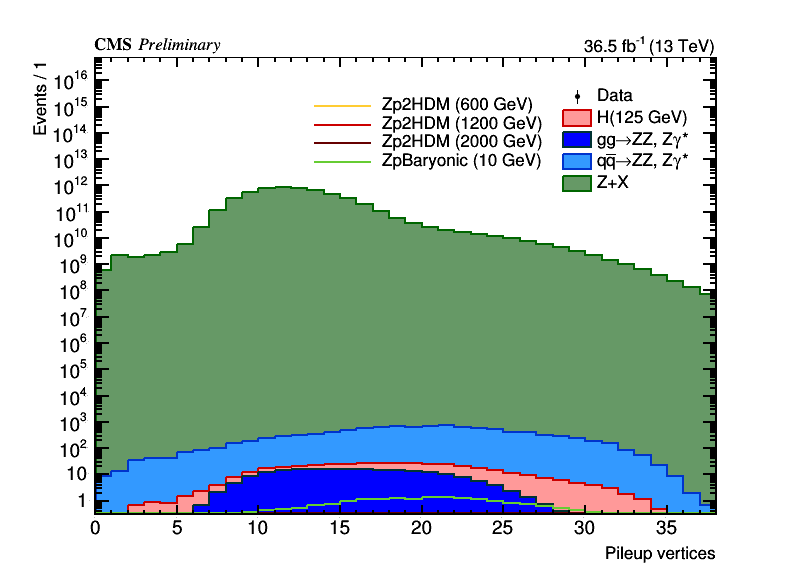
\includegraphics[width=3.25in]{figures/hist_hPUvertices.png}
\caption{}
\end{subfigure}
\begin{subfigure}{0.5\textwidth}
\centering
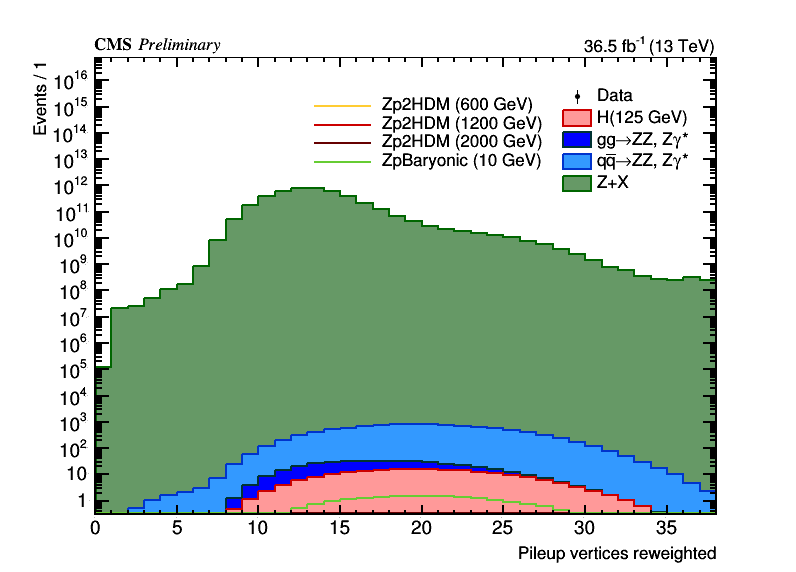
\includegraphics[width=3.25in]{figures/hist_hPUvertices_ReWeighted.png}
\caption{}
\end{subfigure}
\caption{(Number of pileup vertices before (a) and after (b) reweighting is applied.}
\label{fig:pu}
\end{figure}



%The Summer16 Monte Carlo samples are reweighted  to match the pileup distribution in 2016 data. 
%The pileup weights are shown in Fig.~\ref{fig:PUrew} (right). They were computed from a Monte-Carlo pileup profile obtained directly from the 25ns 76X MC production parameter file, and a data pileup profile obtained using the rereco 50ns JSON file ($77\ \text{pb}^{-1}$) and the 25ns Silver JSON file ($2.63\ \text{fb}^{-1}$, taking $69\ \text{mb}^{-1}$). These profiles are shown in Fig.~\ref{fig:PUrew} (left).

%A closure test was performed with events preselected with the requirement of a Z candidate (Fig.~\ref{fig:PUrewtest}), showing a much better agreement in the distribution of the number of vertices when the reweighting is applied.
%The reweighting was found to increase the expected yield in the signal region by 0.4\%.


%=======
%\begin{figure}[!htb]
%\vspace*{0.3cm}
%\begin{center}
%\includegraphics[width=0.45\textwidth]{Figures/pileup76x50ns25nsSilver}
%\includegraphics[width=0.45\textwidth]{Figures/puweight76x50ns25nsSilver}
%\caption{(left) Data and Monte-Carlo pileup profiles that were used to compute the weights. (right) Pileup weights that are applied to simulation events.
%\label{fig:PUrew}}
%\end{center}
%\end{figure}
%=======

%=======
%\begin{figure}[!htb]
%\vspace*{0.3cm}
%\begin{center}
%\includegraphics[width=0.45\textwidth]{Figures/c_CheckPUReweighting_}
%\caption{Closure test: distribution of the number of vertices in simulation before and after reweighting compared to that in data, for a set of events containing a Z candidate as defined in Section~\ref{sec:zzcandsel}.
%\label{fig:PUrewtest}}
%\end{center}
%\end{figure}
%%=======


%\chapter{Datasets and Monte Carlo Simulations}

\section{Data}

\subsection{Triggers and Datasets}
\label{sec:trigpaths}

This analysis uses a data sample recorded by the CMS experiment during 2016, corresponding to $\usedLumi$ of data. 
The datasets are listed in Table~\ref{tab:datasets_data}, along with the integrated luminosity.  
The analysis relies on five different primary datasets (PDs), 
{\it DoubleEG}, {\it DoubleMuon}, {\it MuEG}, {\it SingleElectron}, and {\it SingleMuon},
each of which combines a certain collection of HLT paths. 
To avoid duplicate events from different primary datasets, events are taken:
\begin{itemize}
\item from DoubleEG if they pass the diEle or triEle triggers,
\item from DoubleMuon if they pass the diMuon or triMuon triggers and fail the diEle and triEle triggers,
\item from MuEG if they pass the MuEle or MuDiEle or DiMuEle triggers and fail the diEle, triEle, diMuon and triMuon triggers,
\item from SingleElectron if they pass the singleElectron trigger and fail all the above triggers. 
\item from SingleMuon if they pass the singleMuon trigger and fail all the above triggers. 
\end{itemize} 

The HLT paths used for 2016 collision data are listed in Table~\ref{tab:triggerPaths}, 
together with their L1 seed, prescale value and the associated primary dataset.

%The JSON files are the following:
%\begin{itemize}
%\item Cert\_13TeV\_16Dec2015ReReco\_Collisions15\_50ns\_JSON.txt (for 50 ns data),
%\item Cert\_13TeV\_16Dec2015ReReco\_Collisions15\_25ns\_JSON\_Silver.txt (for 25 ns data).
%\end{itemize} 

\begin{table}[h]
\tiny
    \centering
    \begin{tabular}{|l|l|l|} 
\hline %----------------------------------------------------------------------------------------
\hline %---------------------------------------------------------------------------------------- 
Run-range & Dataset & Integrated luminosity \\
\hline %----------------------------------------------------------------------------------------
\hline %---------------------------------------------------------------------------------------- 
\multirow{5}{*}{273150-275376} & /DoubleMuon/Run2016B-23Sep2016-v3/AOD &  \multirow{5}{*}{$5.892\ \text{fb}^{-1}$} \\ 
& /DoubleEG/Run2016B-23Sep2016-v3/AOD &  \\ 
& /MuonEG/Run2016B-23Sep2016-v3/AOD &  \\ 
& /SingleElectron/Run2016B-23Sep2016-v3/AOD &  \\ 
& /SingleMuon/Run2016B-23Sep2016-v3/AOD &  \\ 
\hline
\multirow{5}{*}{275656-276283} & /DoubleMuon/Run2016C-23Sep2016-v1/AOD &  \multirow{5}{*}{$2.646\ \text{fb}^{-1}$}  \\ 
& /DoubleEG/Run2016C-23Sep2016-v1/AOD &  \\ 
& /MuonEG/Run2016C-23Sep2016-v1/AOD &  \\ 
& /SingleElectron/Run2016C-23Sep2016-v1/AOD &  \\ 
& /SingleMuon/Run2016C-23Sep2016-v1/AOD &  \\ 
\hline
\multirow{5}{*}{276315-276811} & /DoubleMuon/Run2016D-23Sep2016-v1/AOD &  \multirow{5}{*}{$4.353\ \text{fb}^{-1}$} \\ 
& /DoubleEG/Run2016D-23Sep2016-v1/AOD &  \\ 
& /MuonEG/Run2016D-23Sep2016-v1/AOD &  \\ 
& /SingleElectron/Run2016D-23Sep2016-v1/AOD &  \\ 
& /SingleMuon/Run2016D-23Sep2016-v1/AOD &  \\ 
\hline
\multirow{5}{*}{276831-277420} & /DoubleMuon/Run2016E-23Sep2016-v1/AOD &  \multirow{5}{*}{$4.117\ \text{fb}^{-1}$} \\ 
& /DoubleEG/Run2016E-23Sep2016-v1/AOD &  \\ 
& /MuonEG/Run2016E-23Sep2016-v1/AOD &  \\ 
& /SingleElectron/Run2016E-23Sep2016-v1/AOD &  \\ 
& /SingleMuon/Run2016E-23Sep2016-v1/AOD &  \\ 
\hline
\multirow{5}{*}{277932-278808} & /DoubleMuon/Run2016F-23Sep2016-v1/AOD &  \multirow{5}{*}{$3.186\ \text{fb}^{-1}$} \\ 
& /DoubleEG/Run2016F-23Sep2016-v1/AOD &  \\ 
& /MuonEG/Run2016F-23Sep2016-v1/AOD &  \\ 
& /SingleElectron/Run2016F-23Sep2016-v1/AOD &  \\ 
& /SingleMuon/Run2016F-23Sep2016-v1/AOD &  \\ 
\hline
\multirow{5}{*}{278820-280385} & /DoubleMuon/Run2016G-23Sep2016-v1/AOD &  \multirow{5}{*}{$7.721\ \text{fb}^{-1}$} \\ 
& /DoubleEG/Run2016G-23Sep2016-v1/AOD &  \\ 
& /MuonEG/Run2016G-23Sep2016-v1/AOD &  \\ 
& /SingleElectron/Run2016G-23Sep2016-v1/AOD &  \\ 
& /SingleMuon/Run2016G-23Sep2016-v1/AOD &  \\ 
\hline
\multirow{15}{*}{281207-284068} & /DoubleMuon/Run2016H-PromptReco-v1/AOD &  \multirow{15}{*}{$8.857\ \text{fb}^{-1}$} \\ 
& /DoubleEG/Run2016H-PromptReco-v1/AOD &  \\ 
& /MuonEG/Run2016H-PromptReco-v1/AOD &  \\ 
& /SingleElectron/Run2016H-PromptReco-v1/AOD &  \\ 
& /SingleMuon/Run2016H-PromptReco-v1/AOD &  \\ 
& /DoubleMuon/Run2016H-PromptReco-v2/AOD &  \\ 
& /DoubleEG/Run2016H-PromptReco-v2/AOD &  \\ 
& /MuonEG/Run2016H-PromptReco-v2/AOD &  \\ 
& /SingleElectron/Run2016H-PromptReco-v2/AOD &  \\ 
& /SingleMuon/Run2016H-PromptReco-v2/AOD &  \\ 
& /DoubleMuon/Run2016H-PromptReco-v3/AOD &  \\ 
& /DoubleEG/Run2016H-PromptReco-v3/AOD &  \\ 
& /MuonEG/Run2016H-PromptReco-v3/AOD &  \\ 
& /SingleElectron/Run2016H-PromptReco-v3/AOD &  \\ 
& /SingleMuon/Run2016H-PromptReco-v3/AOD &  \\ 
\hline %----------------------------------------------------------------------------------------
\hline %----------------------------------------------------------------------------------------
     \end{tabular}
%\small
    \caption{ Datasets used in the analysis. }
    \label{tab:datasets_data}
\end{table}


\begin{table}[h]
\tiny
    \centering
    \begin{tabular}{|l|l|c|l|} 
\hline %--------------------------------------------------------------------------------------------------------------------------
HLT path                      				       & L1 seed                          & prescale  & primary dataset \\
\hline %--------------------------------------------------------------------------------------------------------------------------
\verb| HLT_Ele17_Ele12_CaloIdL_TrackIdL_IsoVL_DZ       | & \verb| L1_DoubleEG_15_10    |  & 1 & DoubleEG \\
\verb| HLT_Ele23_Ele12_CaloIdL_TrackIdL_IsoVL_DZ       | & \verb| L1_DoubleEG_22_10    |  & 1 & DoubleEG \\
\verb| HLT_DoubleEle33_CaloIdL_GsfTrkIdVL              | & \verb| (Multiple)           |  & 1 & DoubleEG \\
\verb| HLT_Ele16_Ele12_Ele8_CaloIdL_TrackIdL           | & \verb| L1_TripleEG_14_10_8  |  & 1 & DoubleEG \\
\verb| HLT_Mu17_TrkIsoVVL_Mu8_TrkIsoVVL                | & \verb| L1_DoubleMu_11_4     |  & 1 & DoubleMuon \\
\verb| HLT_Mu17_TrkIsoVVL_TkMu8_TrkIsoVVL              | & \verb| L1_DoubleMu_11_4     |  & 1 & DoubleMuon \\
\verb| HLT_TripleMu_12_10_5                            | & \verb| L1_TripleMu_5_5_3    |  & 1 & DoubleMuon \\
\verb| HLT_Mu8_TrkIsoVVL_Ele17_CaloIdL_TrackIdL_IsoVL  | & \verb| L1_Mu5_EG15          |  & 1 & MuonEG \\
\verb| HLT_Mu8_TrkIsoVVL_Ele23_CaloIdL_TrackIdL_IsoVL  | & \verb| L1_Mu5_EG20          |  & 1 & MuonEG \\
\verb| HLT_Mu17_TrkIsoVVL_Ele12_CaloIdL_TrackIdL_IsoVL | & \verb| L1_Mu12_EG10         |  & 1 & MuonEG \\
\verb| HLT_Mu23_TrkIsoVVL_Ele12_CaloIdL_TrackIdL_IsoVL | & \verb| L1_Mu20_EG10         |  & 1 & MuonEG \\
\verb| HLT_Mu23_TrkIsoVVL_Ele8_CaloIdL_TrackIdL_IsoVL  | & \verb| L1_SingleMu*         |  & 1 & MuonEG \\
\verb| HLT_Mu8_DiEle12_CaloIdL_TrackIdL                | & \verb| L1_Mu6_DoubleEG10    |  & 1 & MuonEG \\
\verb| HLT_DiMu9_Ele9_CaloIdL_TrackIdL                 | & \verb| L1_DoubleMu7_EG7     |  & 1 & MuonEG \\
\verb| HLT_Ele25_eta2p1_WPTight                        | & \verb| L1_SingleEG*         |  & 1 & SingleElectron \\
\verb| HLT_Ele27_WPTight                               | & \verb| L1_SingleEG*         |  & 1 & SingleElectron \\
\verb| HLT_Ele27_eta2p1_WPLoose_Gsf                    | & \verb| L1_SingleEG*         |  & 1 & SingleElectron \\
\verb| HLT_IsoMu20 OR HLT_IsoTkMu20                    | & \verb| L1_SingleMu*         |  & 1 & SingleMuon \\
\verb| HLT_IsoMu22 OR HLT_IsoTkMu22                    | & \verb| L1_SingleMu*         |  & 1 & SingleMuon \\
\hline %--------------------------------------------------------------------------------------------------------------------------
    \end{tabular}
%\small
    \caption{Trigger paths used in 2016 collision data.}
    \label{tab:triggerPaths}
\end{table}


\subsection{Trigger Efficiency}

The efficiency in data of the combination of triggers used in the anlysis with respect to the offline reconstruction and selection is measured
by considering 4$\ell$ events triggered by single lepton triggers. One of the four reconstructed leptons ( the ``tag'') is geometrically matched 
to a trigger object passing the final filter of one of the single muon or single electron triggers. The other three leptons are 
used as ``probes''. In each 4$\ell$ event there are up to 4 possible tag-probe combinations, and all possible combinations are counted in the
denominator of the efficiency. For each of the three probe leptons all matching trigger filter objects are collected. Then the matched trigger filter
objects of the three probe leptons are combined in attempt to reconstruct any of the triggers used in the anlysis. If any of the analysis triggers
can be formed using the probe leptons, the set of probes is also counted in the numerator of the efficiency.

This method does not have a perfect closure in MC events due to the fact that the presence of a fourth lepton increases the trigger efficiency,
and this effect is not accounted for. Also, in the  $2e2\mu$ final state, the three probe leptons cannot be combined to form all possible triggers which 
can collect events with two electrons and two muons (e.g. if the tag lepton is an electron, the three remaining leptons cannot pass a double electron
trigger). Therefore the method is also exercised on MC and the difference between data and MC is used to determine the reliability of the simulation.
 The efficiency plotted as a function of the minimum $p_{\rm{T}}$ of the three probe leptons in data and MC using this method can be seen in 
Fig.\ref{fig:TrigEff}. The MC efficiency describes well the data within the statistical uncertainties.

%=======
\begin{figure}[!htb]
\vspace*{0.3cm}
\begin{center}
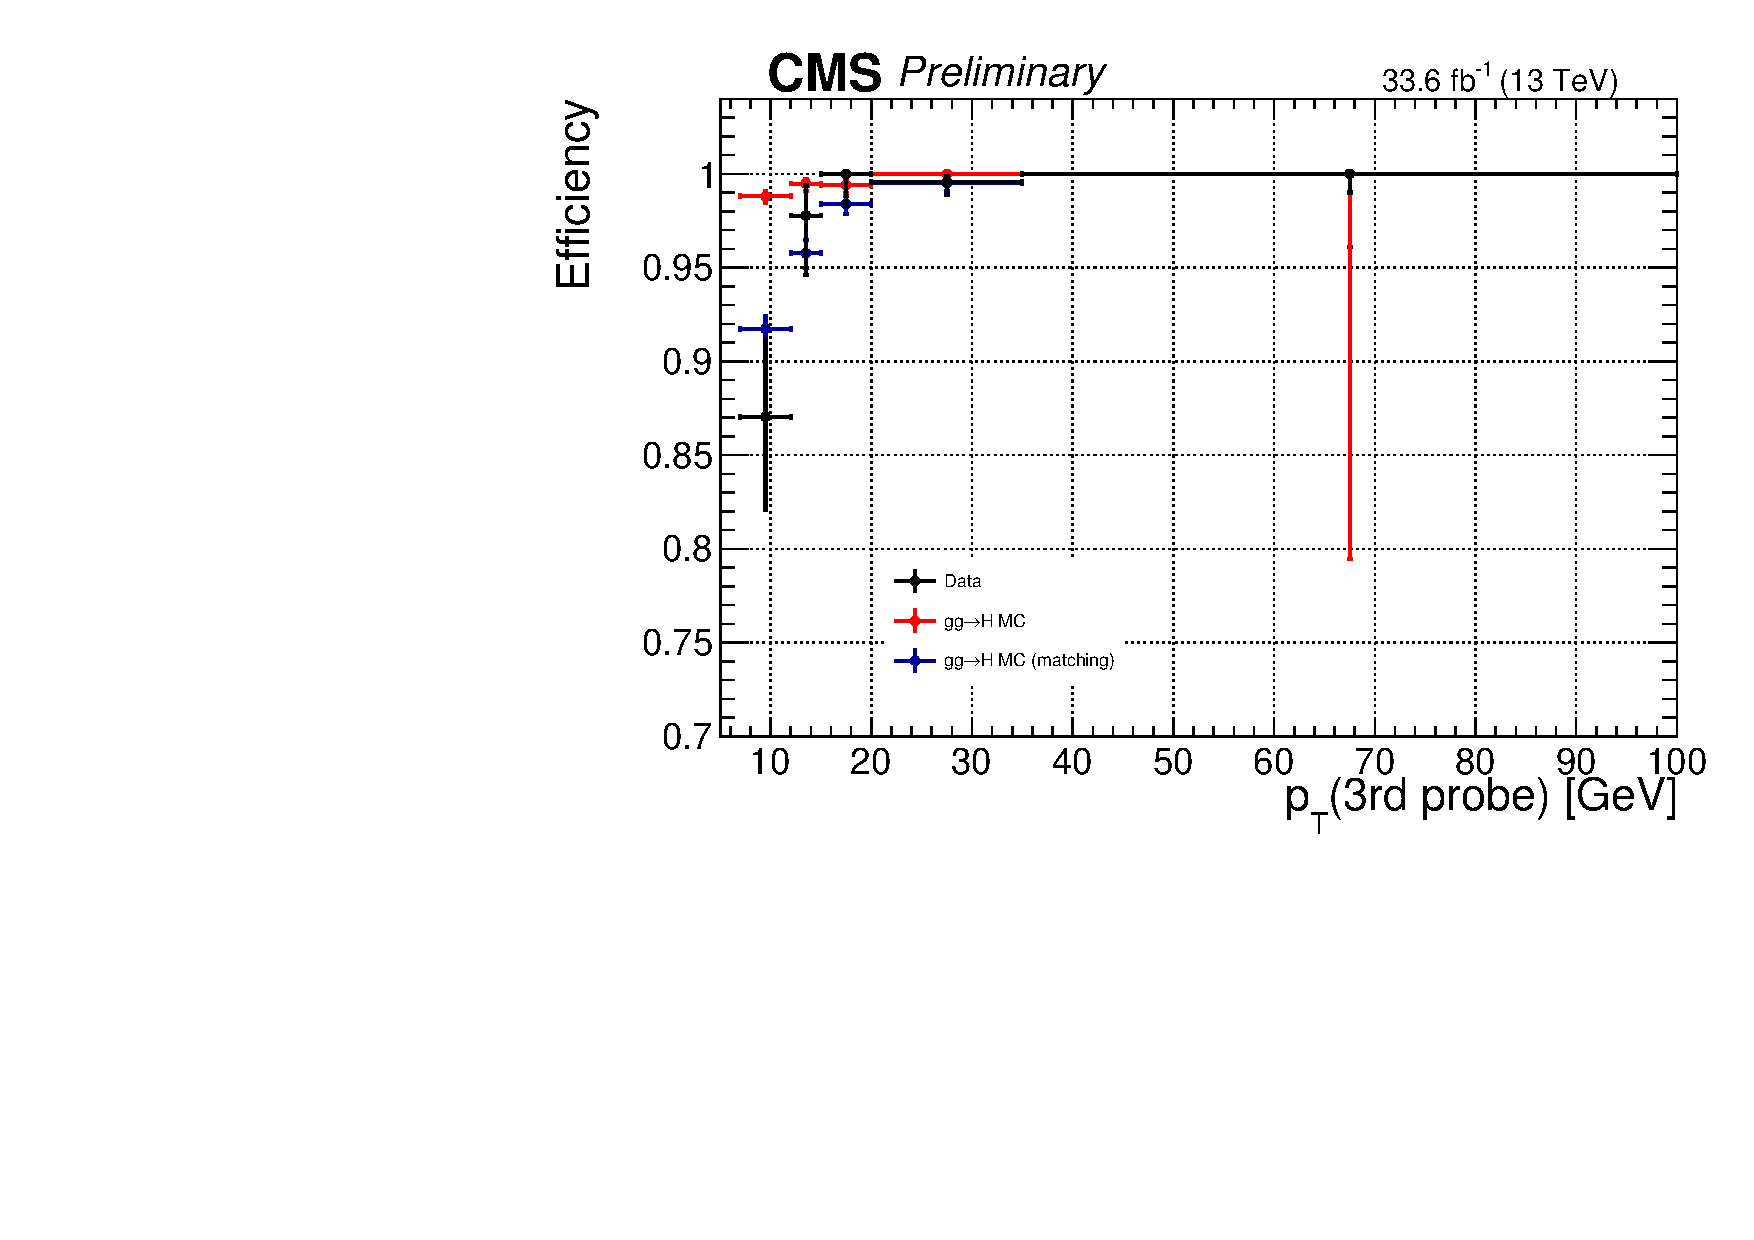
\includegraphics[width=0.45\textwidth]{Figures/Trigger/Histo_TrigEff_ptMin_4e.pdf} 
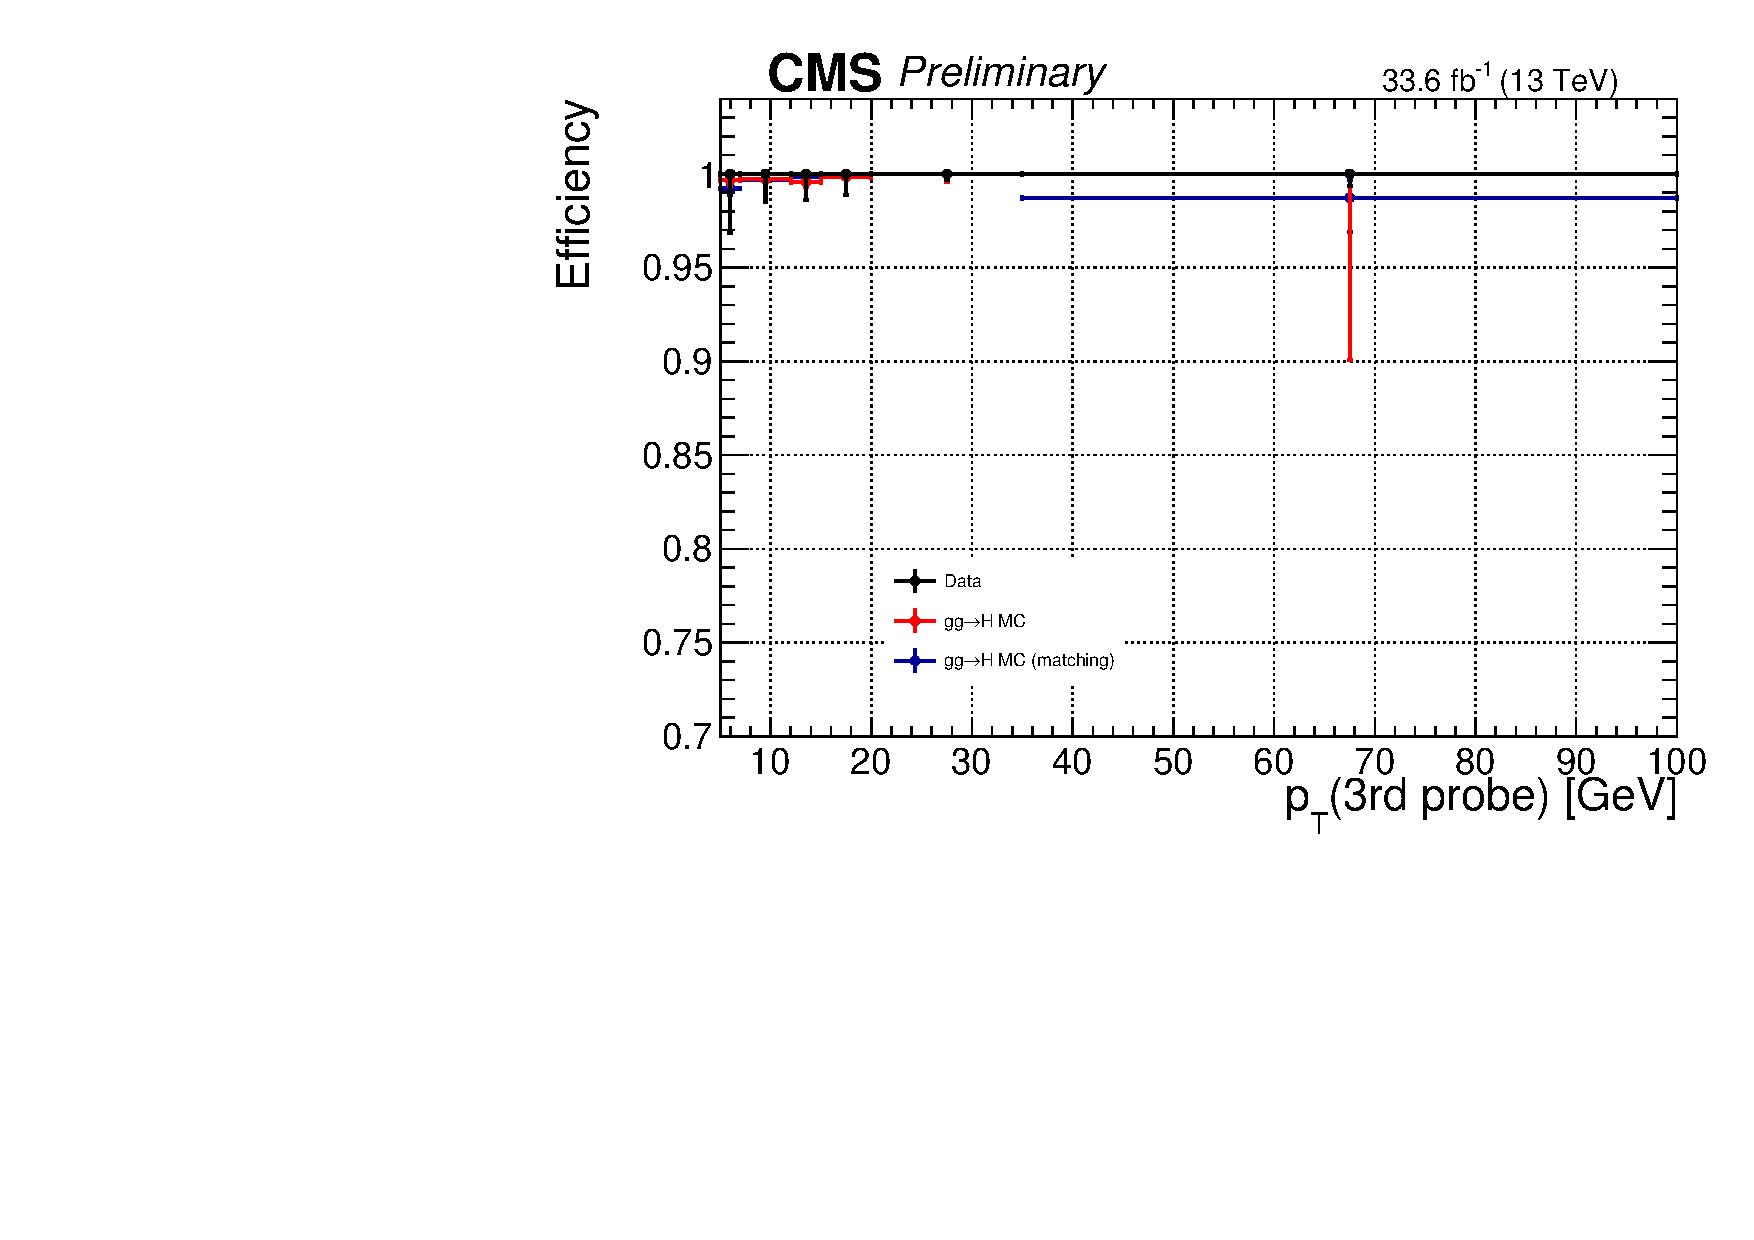
\includegraphics[width=0.45\textwidth]{Figures/Trigger/Histo_TrigEff_ptMin_4mu.pdf} \\
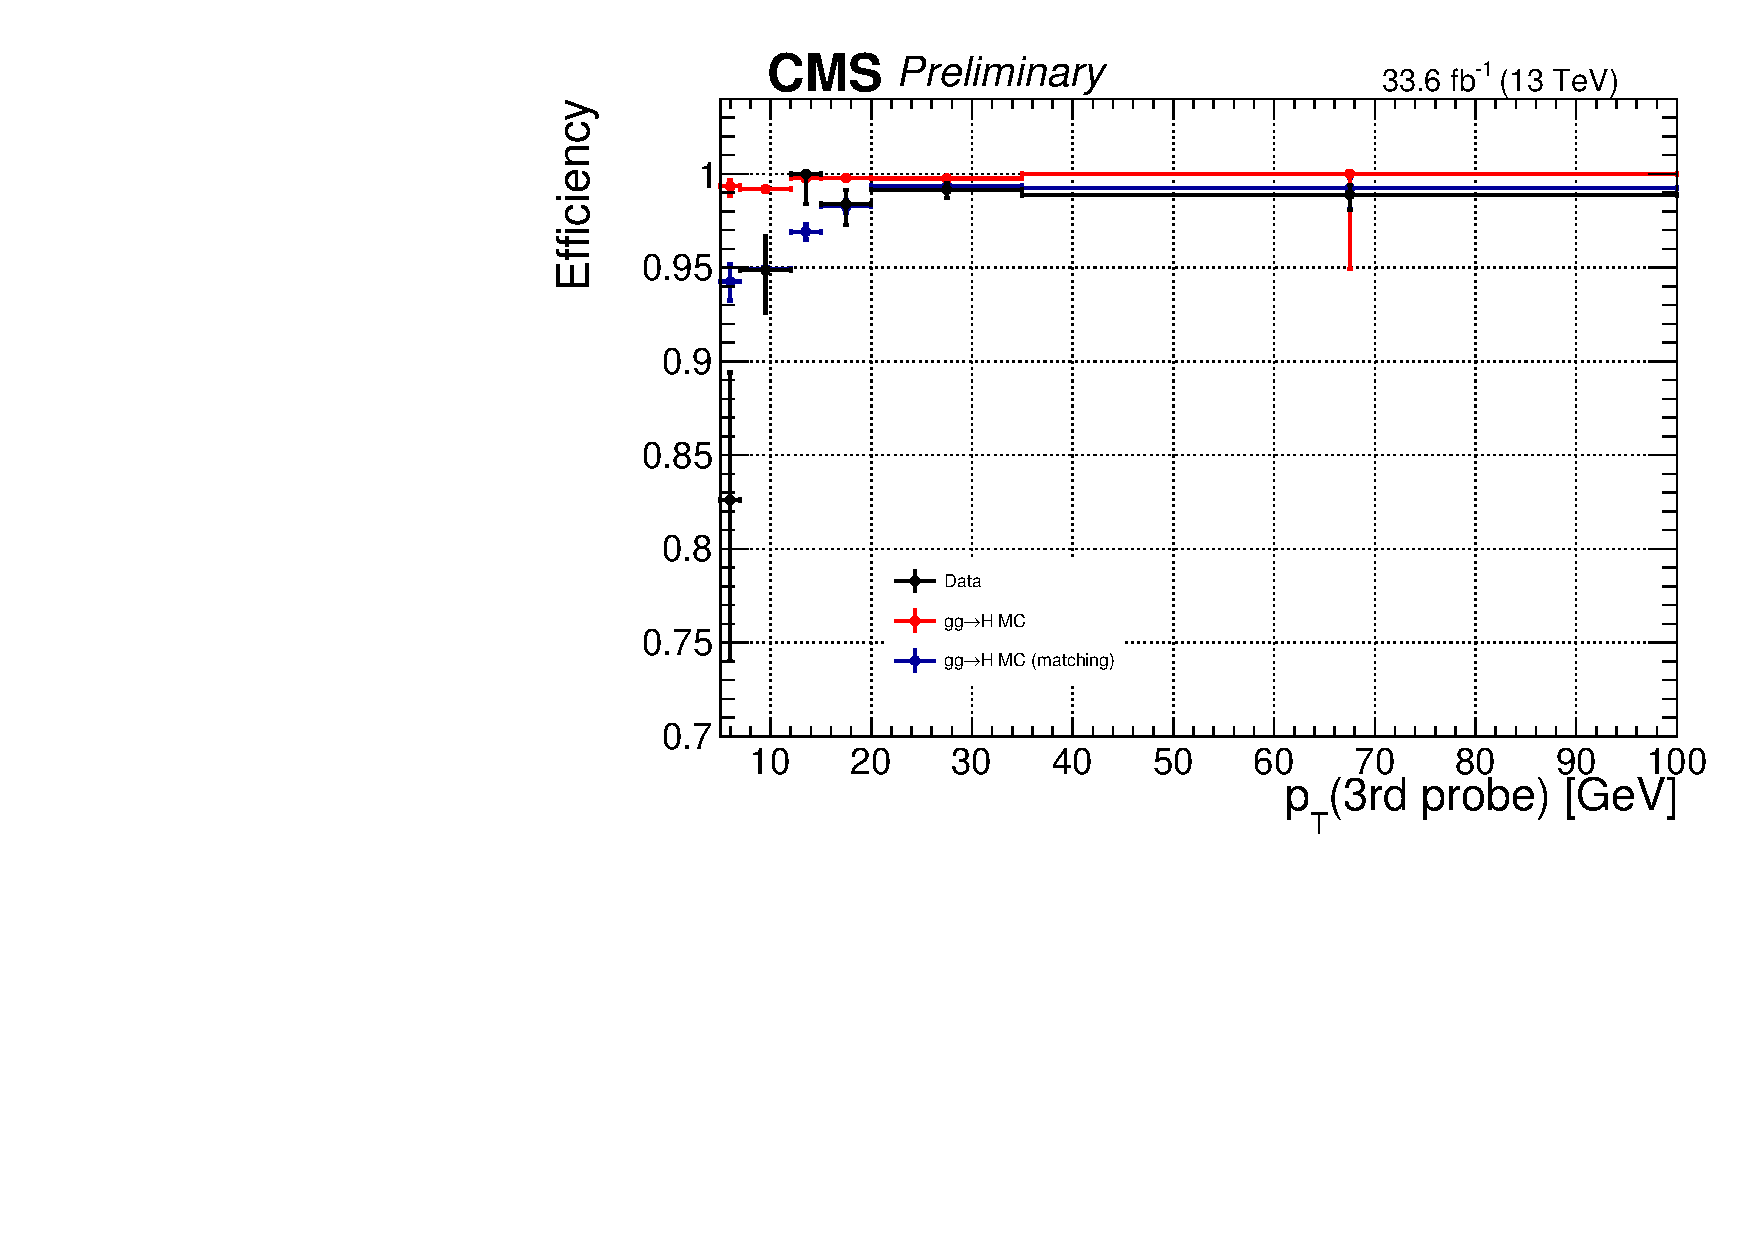
\includegraphics[width=0.45\textwidth]{Figures/Trigger/Histo_TrigEff_ptMin_2e2mu.pdf} 
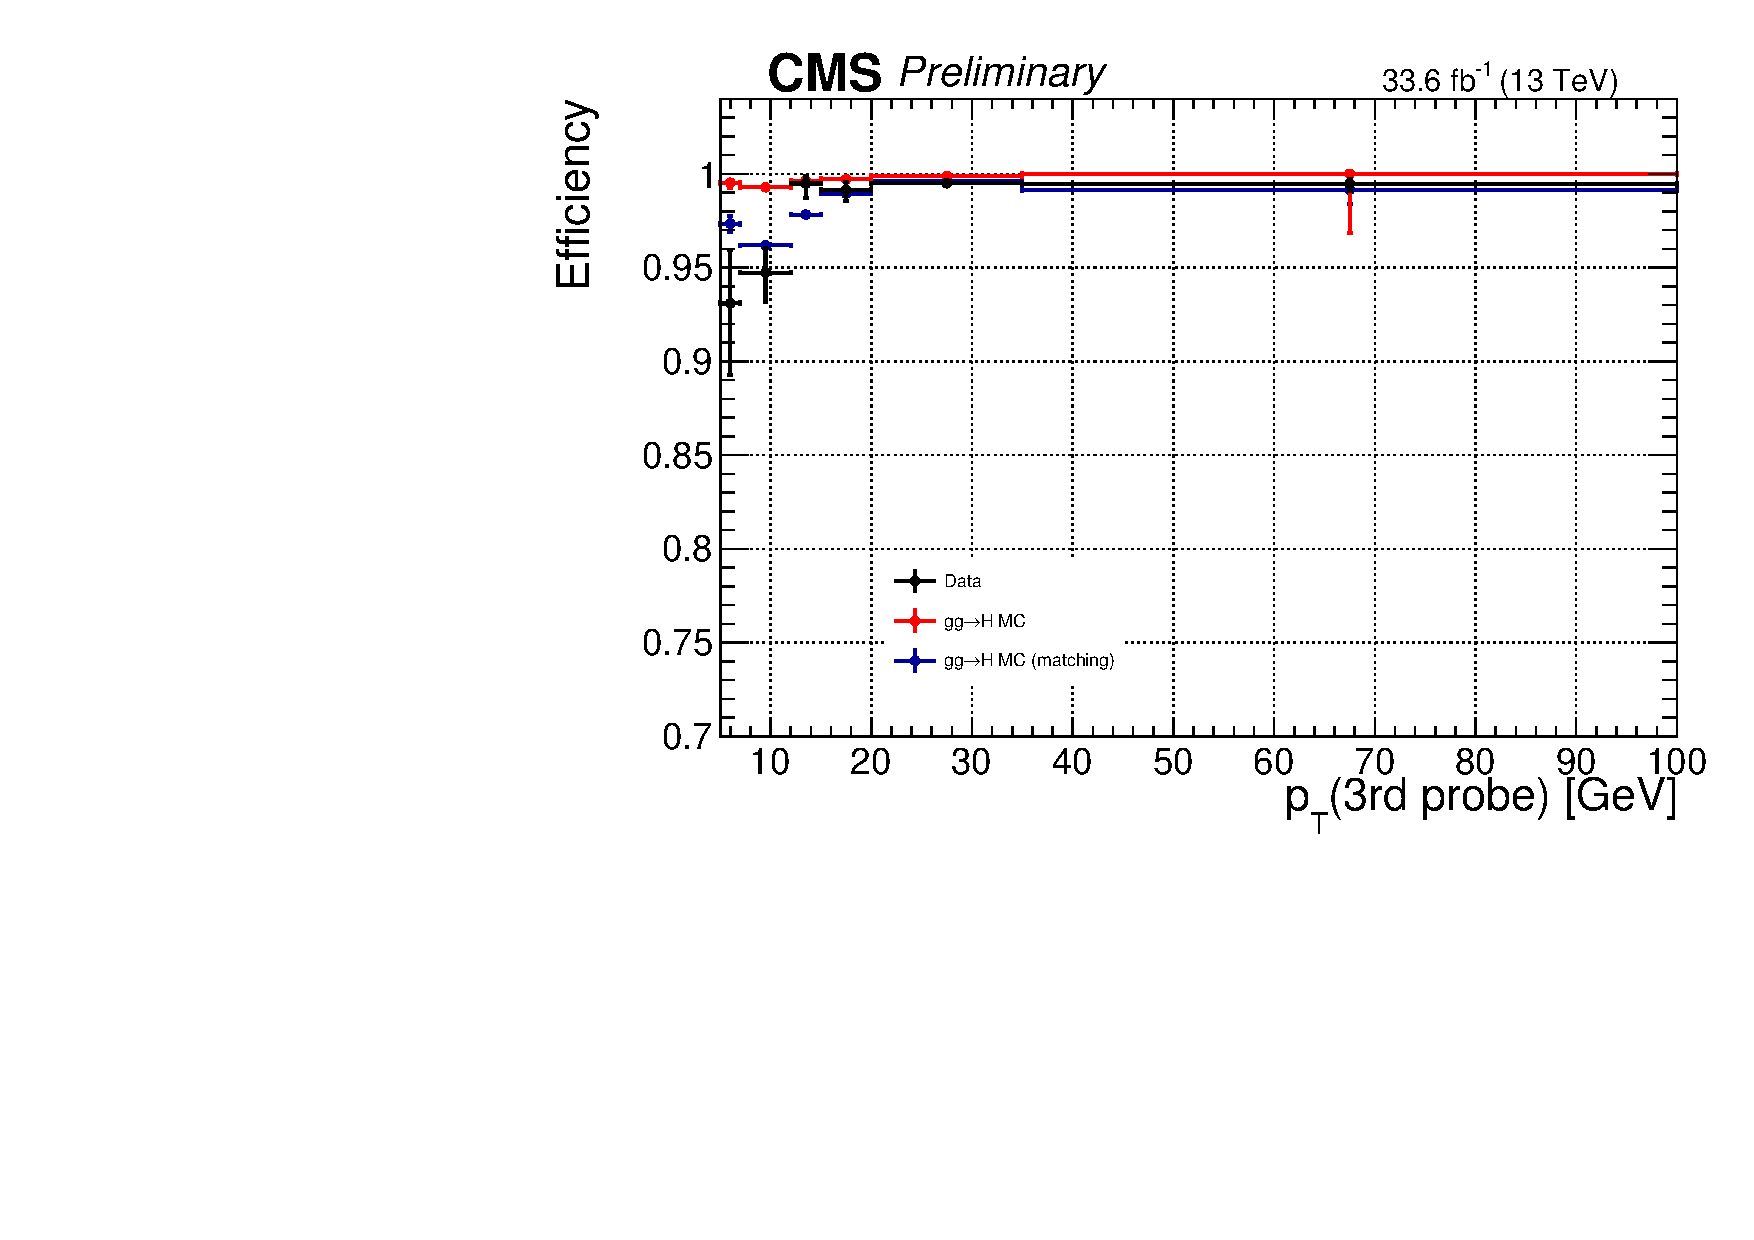
\includegraphics[width=0.45\textwidth]{Figures/Trigger/Histo_TrigEff_ptMin_4l.pdf} \\
\caption{Trigger efficiency measured in data using $4\ell$ events collected by single lepton triggers for the $4e$ (top left), $4\mu$ (top right), $2e2\mu$ (bottom left) and $4\ell$ (bottom right) final states. 
\label{fig:TrigEff}}
\end{center}
\end{figure}
%=======

A summary of the trigger efficiencies in MC truth, and in MC and data using the tag and probe method are summarized in table~\ref{tab:TrigEff}. The trigger
efficiency in simulation is found to be $>99\%$ in each final state.

\begin{table}[h]
    \centering
    \begin{tabular}{|c|c|c|c|c|} 
\hline %----------------------------------------------------------------
Final State  & $\ggH$ MC & $\ggH$ MC (matching)  & Data (matching)   \\
\hline %----------------------------------------------------------------
$4e$  & 0.991$^{+.002}_{-0.002}$ & 0.948$^{+.004}_{-0.004}$ & 0.982$^{+.005}_{-0.007}$ \\
$4\mu$  & 0.997$^{+.001}_{-0.001}$ & 0.997$^{+.001}_{-0.001}$ & 1.000$^{+.000}_{-0.001}$ \\
$2e2\mu$  & 0.995$^{+.001}_{-0.001}$ & 0.964$^{+.002}_{-0.002}$ & 0.983$^{+.003}_{-0.004}$ \\
\hline %----------------------------------------------------------------
    \end{tabular}
    \caption{Trigger efficiencies measured using $4\ell$ events.}
    \label{tab:TrigEff}
\end{table}

\section{Simulation}

\subsection{Signal Samples}

The signal samples used are centrally produced for the benchmarks defined in the previous section and are summarized in Table~\ref{tab:sig}.

\begin{table}
\resizebox{\textwidth}{!}{%
\begin{tabular}{| l | l |}
\hline
Dataset & Parameters\\
\hline
/ZprimeToA0hToA0chichihZZTo4l\_2HDM\_MZp-*\_MA0-300\_13TeV-madgraph-pythia8/[1] & $m_{A^0} = $ 300 GeV \\
/ZprimeToA0hToA0chichihZZTo4l\_2HDM\_MZp-*\_MA0-*\_13TeV-madgraph/[2] & $m_{A^0} \neq $ 300 GeV \\
/MonoHZZ4l\_ZpBaryonic\_MZp-*\_MChi-*\_13TeV-madgraph/[3] & \\
\hline
$[1]$ RunIISpring16DR80-premix\_withHLT\_80X\_mcRun2\_asymptotic\_v14-v1/AODSIM & \\
$[2]$ RunIISpring16reHLT80-PUSpring16RAWAODSIM\_reHLT\_80X\_mcRun2\_asymptotic\_v14-v1/AODSIM & \\
$[3]$ RunIISpring16DR80-premix\_withHLT\_80X\_mcRun2\_asymptotic\_v14-v1/AODSIM & \\
\hline
\end{tabular}}
\caption{Benchmark signal samples analyzed.}\label{tab:sig}
\end{table}

\subsection{Background Samples}

Descriptions of the SM Higgs boson production are obtained using the 
{\sc powheg V2}~\cite{Alioli:2008gx,Nason:2004rx,Frixione:2007vw} generator for the five main production modes: 
gluon fusion ($\ggH$) including quark mass effects~\cite{Bagnaschi:2011tu}, vector boson fusion 
(VBF)~\cite{Nason:2009ai}, and associated production (WH, $\cPZ$H and \ttbar$\,$H~\cite{Hartanto:2015uka}). 
In the case of WH and $\cPZ$H the {\sc MiNLO HVJ} extension of {\sc powheg} is used~\cite{Luisoni:2013kna}. 
The description of the decay of the Higgs boson to four leptons is obtained using the {\sc JHUgen} 
generator~\cite{Gao:2010qx}. In the case of WH, $\cPZ$H and \ttbar$\,$H, the Higgs boson is allowed
to decay to H$\to \cPZ \cPZ \to 2\ell2$X such that 4-lepton events where two leptons originate from 
the decay of associated $\cPZ$, W bosons or top quarks are also taken into account in the simulation. 
Showering of parton-level events is done using {\sc pythia8.209}, and in all cases matching is performed by 
allowing QCD emissions at all energies in the shower and vetoing them afterwards according to the 
{\sc powheg} internal scale. All samples are generated with the NNPDF 3.0 NLO parton distribution 
functions (PDFs)~\cite{Ball:2014uwa}. The list of Higgs signal samples and their cross sections are shown in 
Table~\ref{tab:SignalSamples}.

\begin{table}
\begin{scriptsize}
    \centering
\resizebox{\textwidth}{!}{%
    \begin{tabular}{|l|l|r|}
   \hline
 Process & Dataset Name & $\sigma\times BR (\times\epsilon_{\text{filter}})$ \\ \hline
 $\rm{gg}\to\rm{H}\to\cPZ\cPZ \to 4\ell$ & /GluGluHToZZTo4L\_M125\_13TeV\_powheg2\_JHUgenV6\_pythia8 & $12.18~\rm{fb}$ \\ % & $12.12~\rm{fb}$ \\
 $\rm{qq}\to\rm{Hqq}\to\cPZ\cPZ\rm{qq}\to4\ell qq$ & /VBF\_HToZZTo4L\_M125\_13TeV\_powheg2\_JHUgenV6\_pythia8 & $1.044~\rm{fb}$ \\ % $1.034~\rm{fb}$ \\
 $\rm{q\bar{q}}\to\rm{W^{+}H}\to\rm{W^{+}}\cPZ\cPZ\to4\ell+\rm{X}$ & /WplusH\_HToZZTo4L\_M125\_13TeV\_powheg2-minlo-HWJ\_JHUgenV6\_pythia8 & $0.232~\rm{fb}$ \\ % $0.2339~\rm{fb}$ \\
 $\rm{q\bar{q}}\to\rm{W^{-}H}\to\rm{W^{-}}\cPZ\cPZ\to4\ell+\rm{X}$ & /WminusH\_HToZZTo4L\_M125\_13TeV\_powheg2-minlo-HWJ\_JHUgenV6\_pythia8 & $0.147~\rm{fb}$ \\ % $0.1471~\rm{fb}$ \\
 $\rm{q\bar{q}}\to\cPZ \rm{H}\to\cPZ\cPZ\cPZ\to4\ell+\rm{X}$ & /ZH\_HToZZ\_4LFilter\_M125\_13TeV\_powheg2-minlo-HZJ\_JHUgenV6\_pythia8 & $0.668~\rm{fb}$ \\ % $0.652~\rm{fb}$ \\
 $\rm{gg}\to\rm{ttH} \to\rm{tt}\cPZ\cPZ\to4\ell+\rm{X}$ & /ttH\_HToZZ\_4LFilter\_M125\_13TeV\_powheg\_JHUgen\_pythia8 & $0.393~\rm{fb}$ \\ % $0.337~\rm{fb}$ \\ 
 \hline
 %\multicolumn{3}{l}{[1] RunIISummer16MiniAODv2-PUMoriond17\_80X\_mcRun2\_asymptotic\_2016\_TrancheIV\_v6-v1} \\
 \end{tabular}}
 \caption{Higgs signal samples and cross sections.}
  \label{tab:SignalSamples}
\end{scriptsize}
\end{table}

Production of $ZZ$ via quark-antiquark annihilation is generated at
next-to-leading order (NLO) using {\sc powheg V2}~\cite{Nason:2013ydw}
and {\sc pythia8}, with 
the same settings as for the Higgs signal. As this simulation covers a large
range of ZZ invariant masses, dynamical QCD factorization and renormalization
scales have been chosen, equal to $m_{\cPZ\cPZ}$. 

The $\Pg\Pg \! \to \! ZZ$ process is simulated at leading order (LO) 
with MCFM~\cite{MCFM,Campbell:2013una}. In order to match the 
$\Pg\Pg \! \to \mathrm{H} \to \! ZZ$ transverse momentum spectra predicted 
by {\sc powheg} at NLO, the showering for MCFM samples is performed with 
different {\sc pythia8} settings, allowing only emissions up to the parton-level scale
(``wimpy'' shower).

Although not directly used to model data observations, additional 
MC samples of W$\cPZ$, Drell-Yan+jets, \ttbar, and tribosons are
generated using {\sc MadGraph5\_aMCatNLO}~\cite{Alwall:2014hca} either
inclusively or merging several jet multiplicities, as detailed in the table.
Table~\ref{tab:MCsamples} summarizes the MC simulation datasets used for this analysis. 

\begin{table}
\begin{footnotesize}
    \centering
\resizebox{\textwidth}{!}{%
    \begin{tabular}{|l|l|r|}
   \hline
 Process & Dataset Name & $\sigma\cdot BR$ \\ \hline
 $\rm{qq} \to \cPZ\cPZ \to 4\ell$ & /ZZTo4L\_13TeV\_powheg\_pythia8 & $1.256 \rm{pb}$ \\
 $\rm{qq} \to \cPZ\cPZ \to 4\ell$ & /ZZTo4L\_13TeV-amcatnloFXFX-pythia8 & $1.212 \rm{pb}$ \\
 $\rm{gg} \rightarrow \cPZ\cPZ \to 4e$ & /GluGluToContinToZZTo4e\_13TeV\_MCFM701 & $0.00159 \rm{ pb}$ \\
 $\rm{gg} \rightarrow \cPZ\cPZ \to 4$$\mu$ & /GluGluToContinToZZTo4mu\_13TeV\_MCFM701 & $0.00159 \rm{ pb}$ \\
 $\rm{gg} \rightarrow \cPZ\cPZ \to 4$$\tau$ & /GluGluToContinToZZTo4tau\_13TeV\_MCFM701 & $0.00159 \rm{ pb}$ \\
 $\rm{gg} \rightarrow \cPZ\cPZ \to 2e2$$\mu$ & /GluGluToContinToZZTo2e2mu\_13TeV\_MCFM701 & $0.00319 \rm{ pb}$ \\
 $\rm{gg} \rightarrow \cPZ\cPZ \to 2e2$$\tau$ & /GluGluToContinToZZTo2e2tau\_13TeV\_MCFM701 & $0.00319 \rm{ pb}$ \\
 $\rm{gg} \rightarrow \cPZ\cPZ \to 2$$\mu2$$\tau$ & /GluGluToContinToZZTo2mu2tau\_13TeV\_MCFM701 & $0.00319 \rm{ pb}$ \\ \hline
 $\cPZ \to \ell\ell$ + jets & /DYJetsToLL\_M-50\_TuneCUETP8M1\_13TeV-amcatnloFXFX-pythia8 & $6104 \rm{ pb}$ \\
 $\cPZ \to \ell\ell$ + jets  & /DYJetsToLL\_M-10to50\_TuneCUETP8M1\_13TeV-amcatnloFXFX-pythia8 & $18610 \rm{ pb}$ \\ \hline
 %W$\cPZ \to 3\ell\nu$ & /WZJets\_TuneCUETP8M1\_13TeV-amcatnloFXFX-pythia8/[1] &  $5.29 \rm{pb}$ \\ 
 W$\cPZ \to 3\ell\nu$ & /WZTo3LNu\_TuneCUETP8M1\_13TeV-powheg-pythia8 & $4.430 \rm{ pb}$ \\ \hline
 $t\bar{t}$ & /TTJets\_TuneCUETP8M1\_13TeV-amcatnloFXFX-pythia8 & $815.96 \rm{ pb}$ \\ 
 $t\bar{t} \to 2\ell2\nu 2b$ & /TTTo2L2Nu\_13TeV-powheg &  $87.31 \rm{pb}$ \\ \hline
% WWZ & /WWZ\_TuneCUETP8M1\_13TeV-amcatnlo-pythia8/[2] & $0.1651 \rm{ pb}$ \\
% W\cPZ\cPZ & /WZZ\_TuneCUETP8M1\_13TeV-amcatnlo-pythia8/[2] & $0.05565 \rm{ pb}$ \\
% \cPZ\cPZ\cPZ & /ZZZ\_TuneCUETP8M1\_13TeV-amcatnlo-pythia8/[2] & $0.01398 \rm{ pb}$ \\ \hline
 %\multicolumn{3}{l}{[1] RunIISummer16MiniAODv2-PUMoriond17\_80X\_mcRun2\_asymptotic\_2016\_TrancheIV\_v6-v1} \\
 \end{tabular}}
 \caption{Background Monte Carlo samples and cross sections.}
  \label{tab:MCsamples}
\end{footnotesize}
\end{table}

\subsubsection{Pileup Reweighting}

The MC samples are reweighted to match the pileup distribution measured in 2016 data. Scale factors are measured and applied to each event weight before histograms are filled and yields are calculated, based on the number of pileup vertices present in the event. The mean number of pileup vertices for data measured in 2016 is about 20. Figure~\ref{fig:pu} shows the distributions of the numbers of pileup vertices for data and MC before and after the events are reweighted.

\begin{figure}[tbh]
\centering
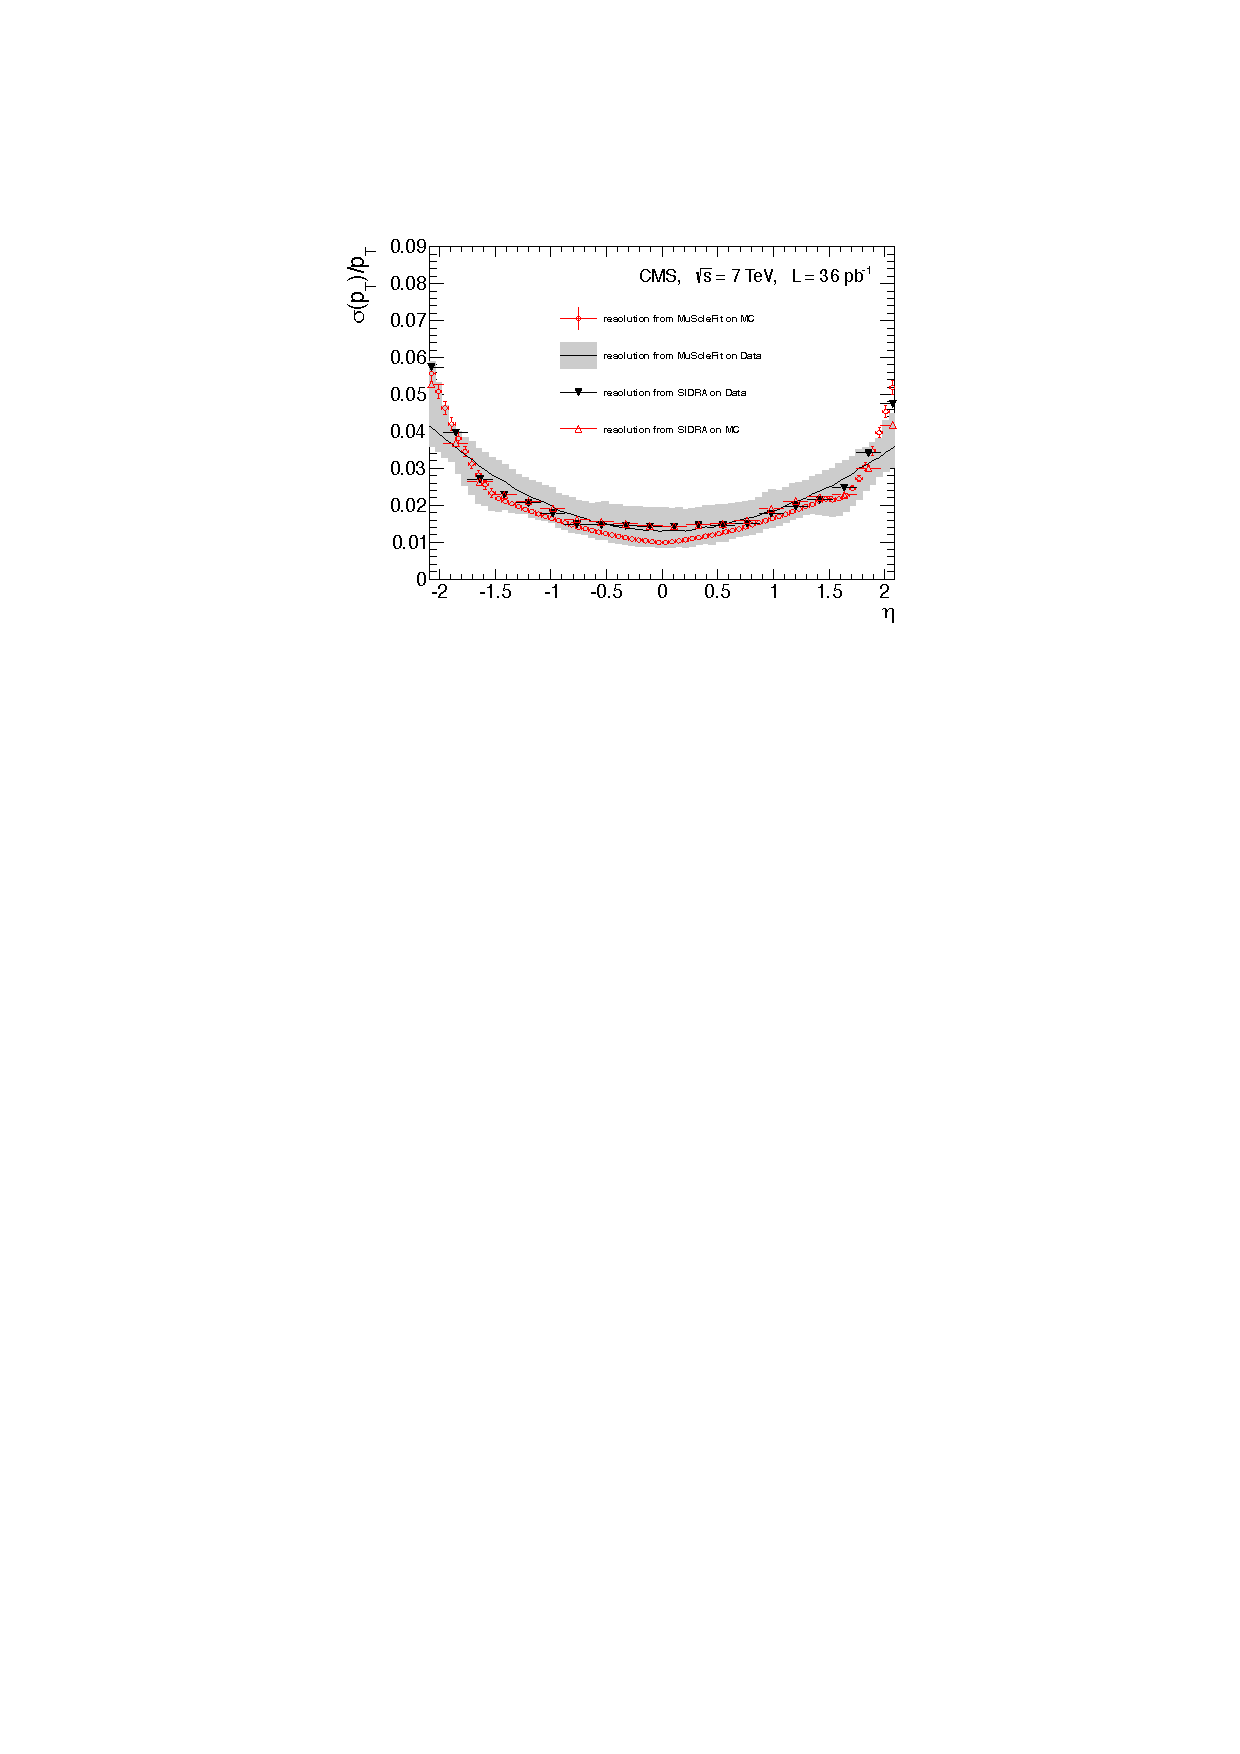
\includegraphics[width=5in]{figures/muonres.pdf}
\caption{Number of pileup vertices before and after reweighted is applied.}
\label{fig:pu}
\end{figure}

%The Summer16 Monte Carlo samples are reweighted  to match the pileup distribution in 2016 data. 
%The pileup weights are shown in Fig.~\ref{fig:PUrew} (right). They were computed from a Monte-Carlo pileup profile obtained directly from the 25ns 76X MC production parameter file, and a data pileup profile obtained using the rereco 50ns JSON file ($77\ \text{pb}^{-1}$) and the 25ns Silver JSON file ($2.63\ \text{fb}^{-1}$, taking $69\ \text{mb}^{-1}$). These profiles are shown in Fig.~\ref{fig:PUrew} (left).

%A closure test was performed with events preselected with the requirement of a Z candidate (Fig.~\ref{fig:PUrewtest}), showing a much better agreement in the distribution of the number of vertices when the reweighting is applied.
%The reweighting was found to increase the expected yield in the signal region by 0.4\%.


%=======
%\begin{figure}[!htb]
%\vspace*{0.3cm}
%\begin{center}
%\includegraphics[width=0.45\textwidth]{Figures/pileup76x50ns25nsSilver}
%\includegraphics[width=0.45\textwidth]{Figures/puweight76x50ns25nsSilver}
%\caption{(left) Data and Monte-Carlo pileup profiles that were used to compute the weights. (right) Pileup weights that are applied to simulation events.
%\label{fig:PUrew}}
%\end{center}
%\end{figure}
%=======

%=======
%\begin{figure}[!htb]
%\vspace*{0.3cm}
%\begin{center}
%\includegraphics[width=0.45\textwidth]{Figures/c_CheckPUReweighting_}
%\caption{Closure test: distribution of the number of vertices in simulation before and after reweighting compared to that in data, for a set of events containing a Z candidate as defined in Section~\ref{sec:zzcandsel}.
%\label{fig:PUrewtest}}
%\end{center}
%\end{figure}
%%=======


\chapter{Physics Objects}\label{sec:objects}

\section{Electrons}

\subsection{Electron Reconstruction}
\label{sec:eleReco}


Electron candidates are preselected using loose cuts on track-cluster matching observables, so as to preserve the highest possible efficiency while rejecting part of the QCD background. To be considered for the analysis, electrons are required to have a
transverse momentum $p^e_T >$ 7 GeV, a reconstructed $|\eta^e| <$ 2.5, and to satisfy a loose primary vertex 
constraint defined as $d_{xy} < 0.5$ and $d_z < 1$. 
Such electrons are called {\bf loose electrons}.

The early runs in the 2016 data-taking exhibit an tracking inefficiency originating from a reduced hit reconstruction efficiency in the strip detector (``HIP" effect). 
The resulting data-MC discrepancy is corrected using scale factors as is done for the electron selection with data efficiencies measured using the same tag-and-probe technique outlined later (see Section~\ref{sec:eleEffMeas}). 
These studies are carried out by the EGM POG and the results are summarized here.

The electron reconstruction scale factors are shown Fig.~\ref{fig:ele_rec_scale_factors} as a one-dimensional function of the super cluster $\eta$ only, as it was shown that the $\pt$ dependence of the scale factor is negligible. More details on electron reconstruction can be found in Ref.~\cite{ElectronLegacy}. 

\begin{figure}[!htb]
\vspace*{0.3cm}
\begin{center}
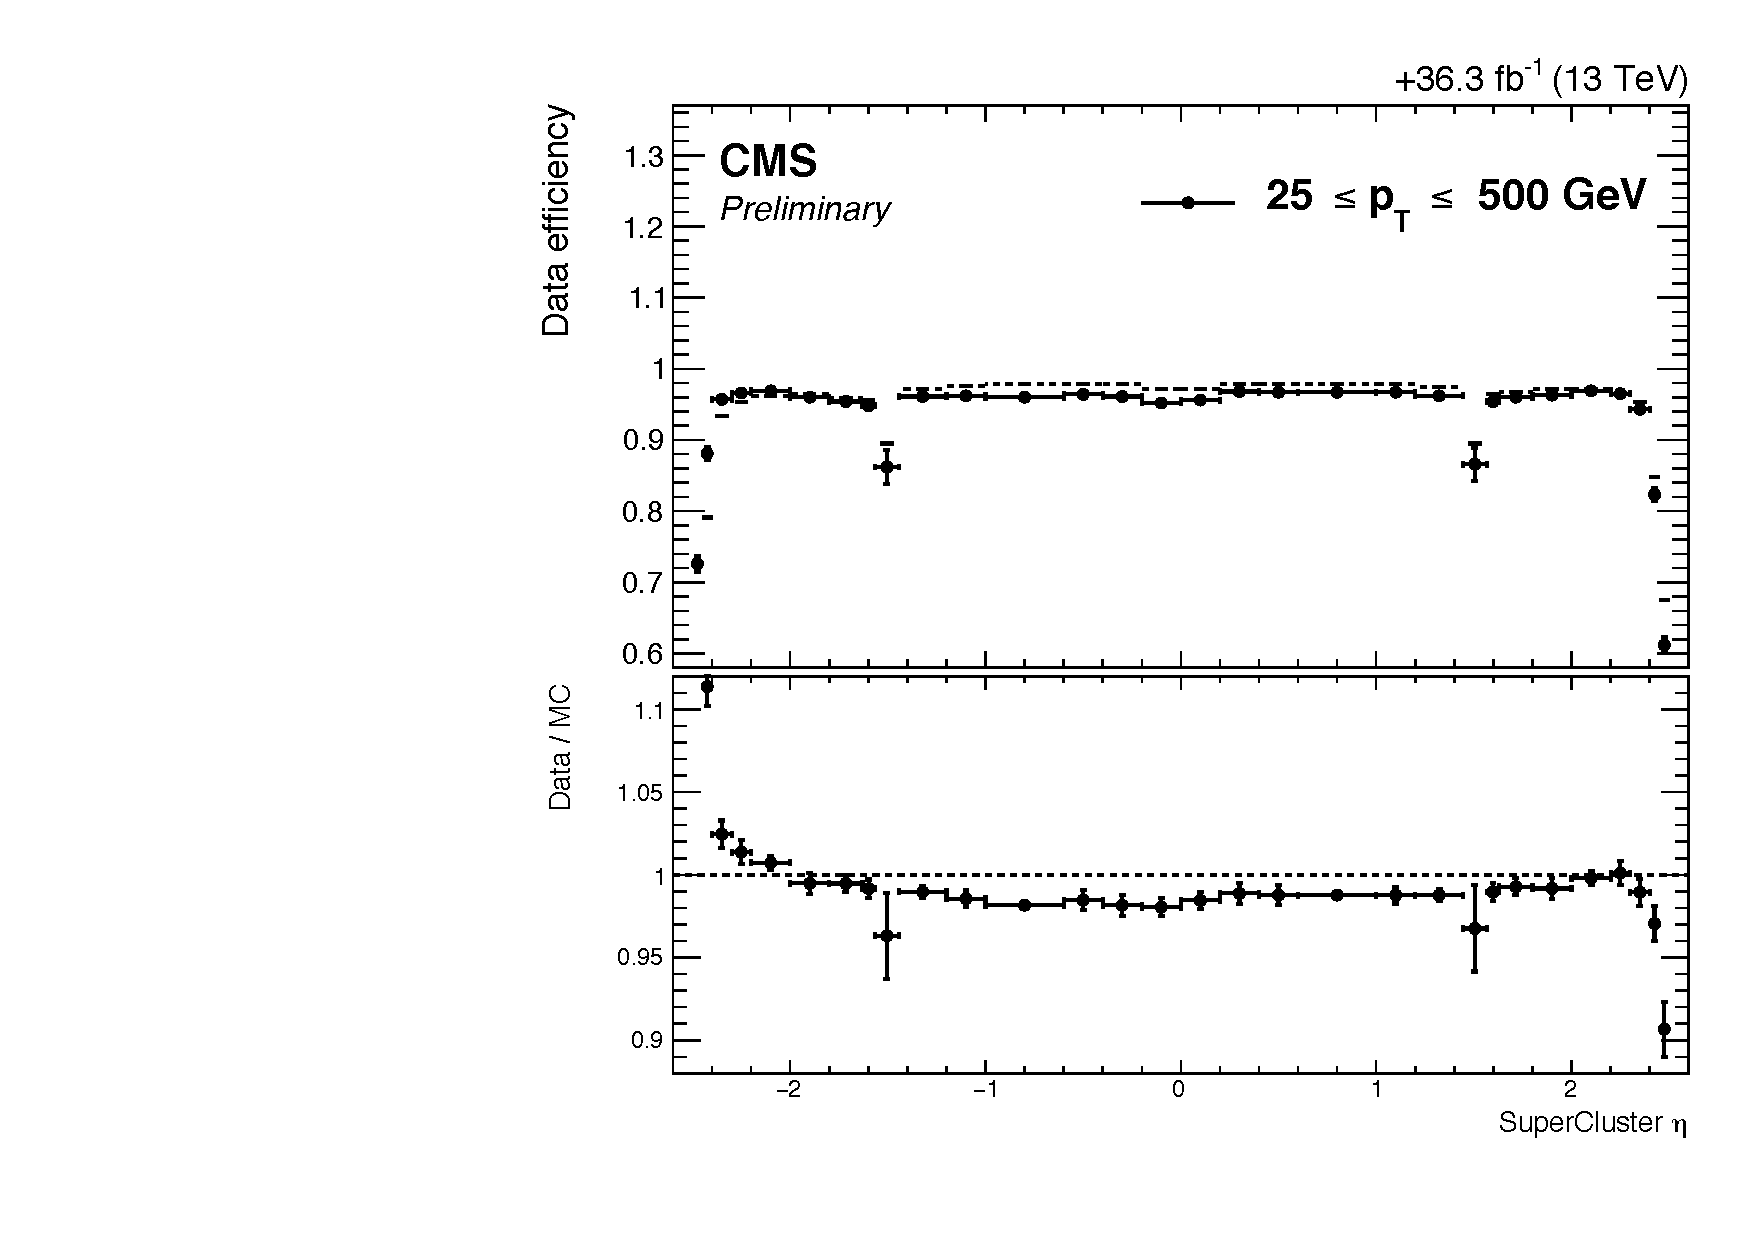
\includegraphics[width=0.6\textwidth]{Figures/Electrons/ele_rec_scale_factors.pdf}
\end{center}
\caption{Electron reconstruction efficiencies efficiency in data versus $\eta$ and data/MC scale factors as provided by the EGM POG.}
\label{fig:ele_rec_scale_factors}
\end{figure}

\subsection{Electron Identification}
\label{sec:eleID}

Reconstructed electrons are identified by means of a Gradient Boosted Decision Tree (GBDT) multivariate classifier algorithm, which exploits observables from the electromagnetic cluster, the matching between the cluster and the electron track as well as observables based exclusively on tracking measurements. 
The BDT has been retrained using CMSSW\_8\_0\_X samples. The classifier is trained on Drell-Yan plus jets MC sample for both signal and background: 

%{
%\resizebox{\textwidth}{!}{%
%\tiny  
%/DYJetsToLL\_M-50\_TuneCUETP8M1\_13TeV-madgraphMLM-pythia8/RunIISpring16DR80-PUSpring16\_80X\_mcRun2\_asymptotic\_2016\_v3\_ext1-v1/
%}}
%{
%\tiny  
%\begin{verbatim}
%/DYJetsToLL_M-50_TuneCUETP8M1_13TeV-madgraphMLM-pythia8/RunIISpring16DR80-PUSpring16_80X_mcRun2_asymptotic_2016_v3_ext1-v1/
%\end{verbatim}
%}

The impact of the retraining of the ID for the 2016 conditions is illustrated in the ROC curves shown in Fig.~\ref{fig:ele_ID_ROC}. Several studies to improve the performance of the MVA for the harsher 2016 running conditions were performed. 
One study considered a new spitting of the BDT training bins, where electrons falling into the gap regions of the ECAL, e.g. the EB-EE transition region, where trained separately from the non-gap electrons. 
No improvement for either population is observed, indicating that the current setup is already able to properly take the significantly differing input distributions in those regions into account. 
Also studied where additional variables including more cluster-shape observables. 
None of these variables helped to improve the performance in the relevant $>95\%$ signal efficiency regime, though up to $20\%$ improved background rejection was seen for $80\%$ working points. 
Finally, the hyper-parameters of the MVA were systematically scanned for their optimal values. The resulting configuration was found to improve the overall performance only marginally by $<10\%$, however, introducing a significant overtraining effect. 
Due to the small gains and large overtraining, it was decided to not modify the hyper-parameters beyond the interface changes coming from changing to the latest 4.2.0 version of the TMVA package.

Figure~\ref{fig:ele_ID_BDT_output} shows the output of the BDT on the training and testing samples for true and fake electrons 
for the high-$p_T$ training bin in the endcap. 
The good agreement between the training and testing distributions is similar across the 6 training bins and indicates that the classifier has not been overtrained.

\begin{figure}[!htb]
\vspace*{0.3cm}
\begin{center}
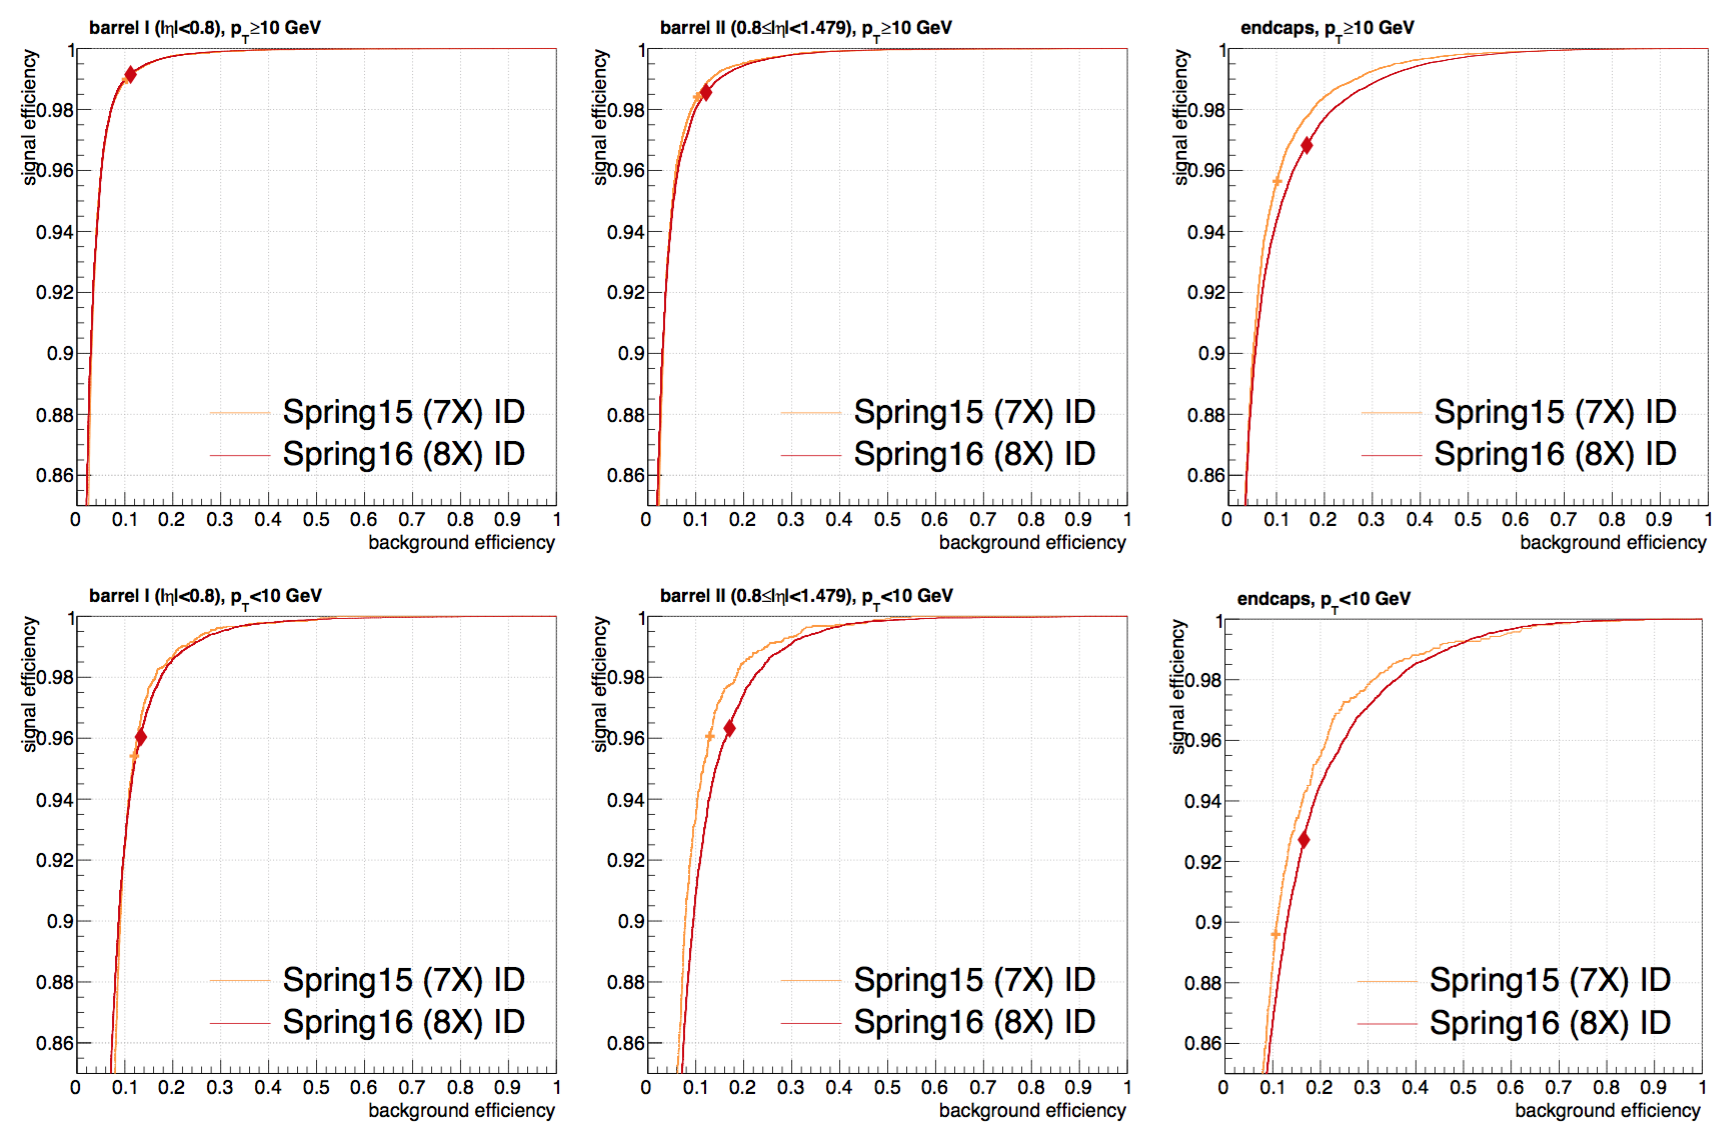
\includegraphics[width=0.80\textwidth]{Figures/Electrons/ele_ROC.png}
\caption{Performance comparison of the MVA trained for the 2015 analysis and the retraining for 2016 conditions. 
The respective working points are indicated by the markers.
\label{fig:ele_ID_ROC}}
\end{center}
\end{figure}

\begin{figure}[!htb]
\vspace*{0.3cm}
\begin{center}
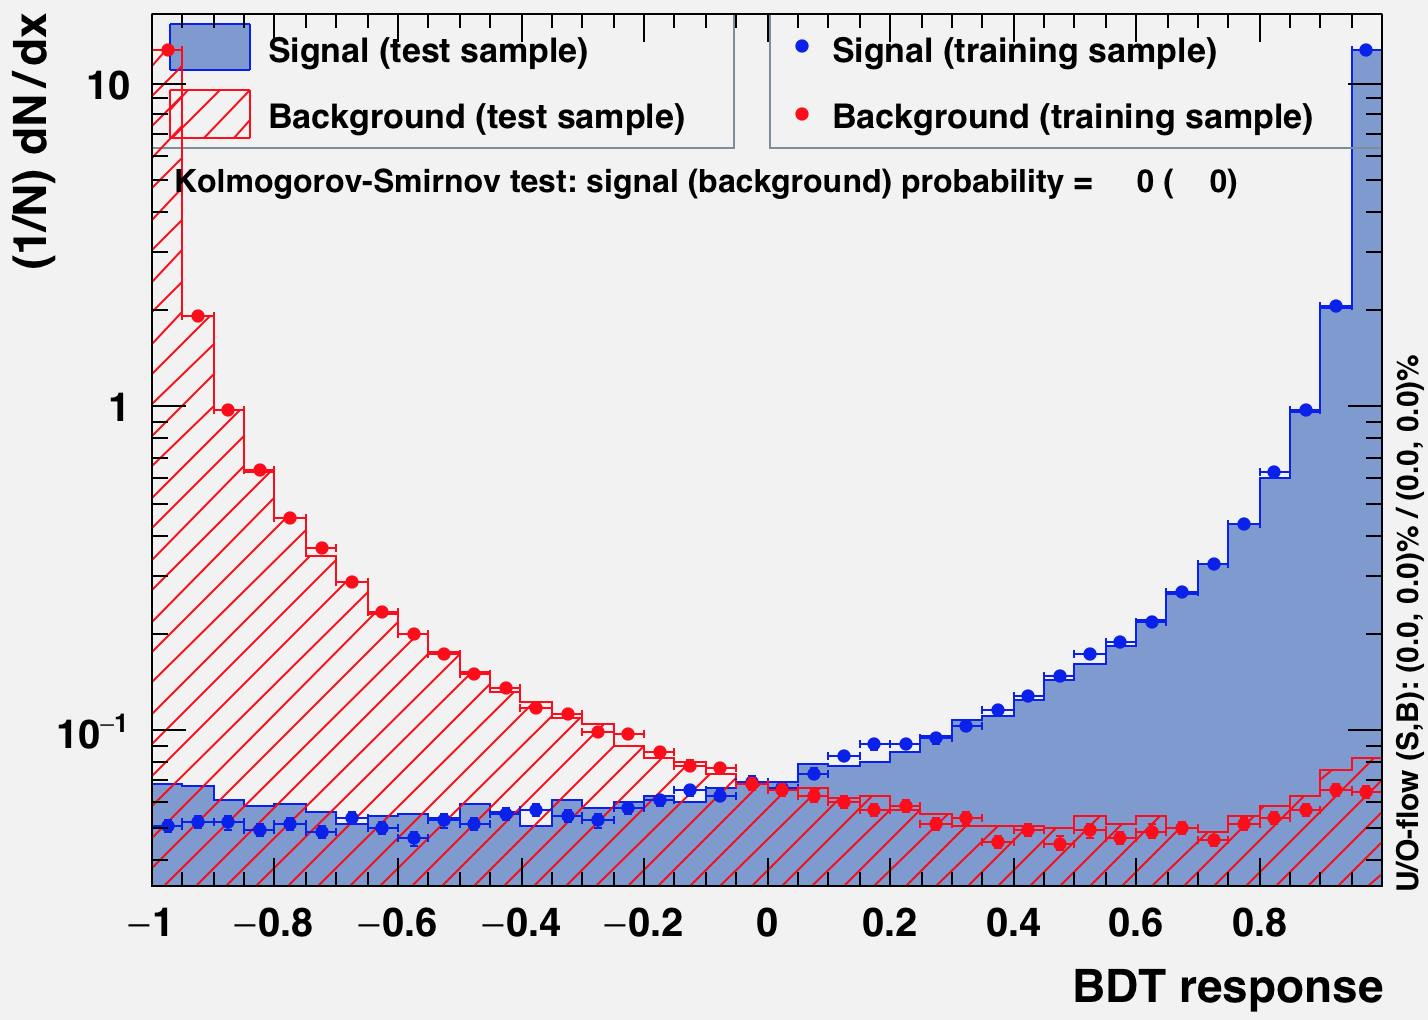
\includegraphics[width=0.5\textwidth]{Figures/Electrons/ele_overtraining.png}
\caption{BDT output for the training and testing sample for true and fake electrons in the high-$p_T$ endcap training bins.
\label{fig:ele_ID_BDT_output}}
\end{center}
\end{figure}

Table~\ref{tab:ele_ID_input_variables} summarizes the full list of observables used as input to the classifier
and table~\ref{tab:ele_ID_WP} lists the cut values applied to the BDT score for the chosen working point. 
For the analysis, we define {\bf tight electrons} as the loose electrons that pass this MVA identification working point. 

 \begin{table}[h!]
\scriptsize
    \centering
\resizebox{\textwidth}{!}{%
    \begin{tabular}{c|l}
\hline %----------------------------------------------------------------------------------------
\hline %----------------------------------------------------------------------------------------
%\multicolumn{4}{|c|}{Datasets}                                                                \\
observable type    &  observable name      	\\
\hline %----------------------------------------------------------------------------------------

\multirow{6}{*}{cluster shape}
	&  RMS of the energy-crystal number spectrum along $\eta$ and $\varphi$; $\sigma_{i\eta i\eta}$, $\sigma_{i\varphi i\varphi}$		\\
	&  super cluster width along $\eta$ and $\phi$		\\
	&  'ratio of the hadronic energy behind the electron 
supercluster to the supercluster energy, $H/E$			\\
	&  circularity $(E_{5\times5} - E_{5\times1})/E_{5\times5}$			\\
	&  sum of the seed and adjacent crystal over the super cluster energy $R_{9}$			\\
	&  for endcap traing bins: energy fraction in pre-shower $E_{PS}/E_{raw}$			\\
\hline
\multirow{2}{*}{track-cluster matching}
	& energy-momentum agreement $E_{tot}/p_{in}$, $E_{ele}/p_{out}$, $1/E_{tot} - 1/p_{in}$ 			\\
	& position matching $\Delta\eta_{in}$, $\Delta\varphi_{in}$, $\Delta\eta_{seed}$			\\
\hline
\multirow{5}{*}{tracking}
        & fractional momentum loss $f_{brem} = 1 - p_{out}/p_{in}$	\\
        & number of hits of the KF and GSF track $N_{KF}$, $N_{GSF}$ $(\mathord{\cdot})$ \\
        & reduced $\chi^2$ of the KF and GSF track $\chi^{2}_{KF}$, $\chi^{2}_{\textrm{GSF}}$ \\
        & number of expected but missing inner hits $(\mathord{\cdot})$ 	\\
        & probability transform of conversion vertex fit $\chi^2$ $(\mathord{\cdot})$ \\

\hline %----------------------------------------------------------------------------------------
\hline %----------------------------------------------------------------------------------------
     \end{tabular}}
%\small
    \caption{Overview of input variables to the identification classifier. Variables not used in the run I MVA are marked with  $(\mathord{\cdot})$.}
    \label{tab:ele_ID_input_variables}
\end{table}


\begin{table}[h!]
\scriptsize
    \centering
    \begin{tabular}{c|c c c}
%\multicolumn{4}{|c|}{Datasets}                                                                \\
\hline %----------------------------------------------------------------------------------------
minimum BDT score    &  $|\eta| < 0.8 $ & $0.8 < |\eta| < 1.479$ 	& $|\eta| > 1.479$      \\
\hline %----------------------------------------------------------------------------------------
$ 5 < p_T < 10 $ GeV &  -0.211      & -0.396  		& -0.215		\\
$p_T > 10$ GeV       &  -0.870		& -0.838		& -0.763		\\
\hline %----------------------------------------------------------------------------------------
\hline %----------------------------------------------------------------------------------------
     \end{tabular}
\small
    \caption{Minimum BDT score required for passing the electron identification.}
    \label{tab:ele_ID_WP}
\end{table}


\subsection{Electron Isolation}
\label{sec:eleiso}

The relative isolation for electrons is defined as: 

\begin{equation}
\text{RelPFiso} = (\sum_{\text{charged}} p_T + \sum^{\text{corr}}_{\text{neutral}} p_T)/p_T^{\text{lepton}}  .
\label{eqn:elepfrelisoeqn}
\end{equation} 

where the corrected neutral component of isolation is computed using the formula :

\begin{equation}
\label{eqn:neutralea}
  \sum^{\text{corr}}_{\text{neutral}} p_T = \text{max}(\sum^{\text{uncorr}}_{\text{neutral}} p_T - \rho \times A_\text{eff},0 \GeV)  .
\end{equation}

and the mean pile-up contribution to the isolation cone is obtained as :  
\begin{equation}
 PU =  \rho \times A_\text{eff}
\label{eqn:purho}
\end{equation}

where $\rho$ is the mean energy density in the event and the effective area $A_{eff}$ is defined as the ratio
between the slope of the average isolation and that of $\rho$ as a function of the number of vertices. 

The electron isolation working point was optimized in Ref.~\cite{AN-15-277} and the electron isolation working was 
chosen to be $\text{RelPFiso}(\Delta R = 0.3) < 0.35$. 


\subsection{Electron Energy Calibrations}

Electrons in data are corrected for features in ECAL energy scale
in bins of $\pt$ and $\left| \eta \right|$. Corrections are calculated
on a $\cPZ \to \Pe\Pe$ sample to align the dielectron 
mass spectrum in the data to that in the MC, and to
minimize its width.

The $\cPZ \to \Pe\Pe$ mass resolution in Monte Carlo is made to match
data by applying a pseudorandom Gaussian smearing to electron energies,
with Gaussian parameters varying in bins of $\pt$ and $\left| \eta \right|$.
This has the effect of convoluting the electron energy spectrum with a
Gaussian.

The electron energy scale is measured in data by fitting a Crystall-ball function to the di-electron mass spectrum around the Z peak in the $Z+\ell$ control region. 
The energy scale for the full 2016 dataset is shown in Fig.~\ref{fig:ele_energy_scale}(a) and agrees with the MC with 100~MeV. 
The stability of the energy scale across different run periods is shown in Fig.~\ref{fig:ele_energy_scale}(b), where the data is binned into approximately 500~pb luminosity blocks.

%\begin{figure}[!htb]
%\vspace*{0.3cm}
%\begin{center}
%\subfigure [] {\resizebox{7.5cm}{!}{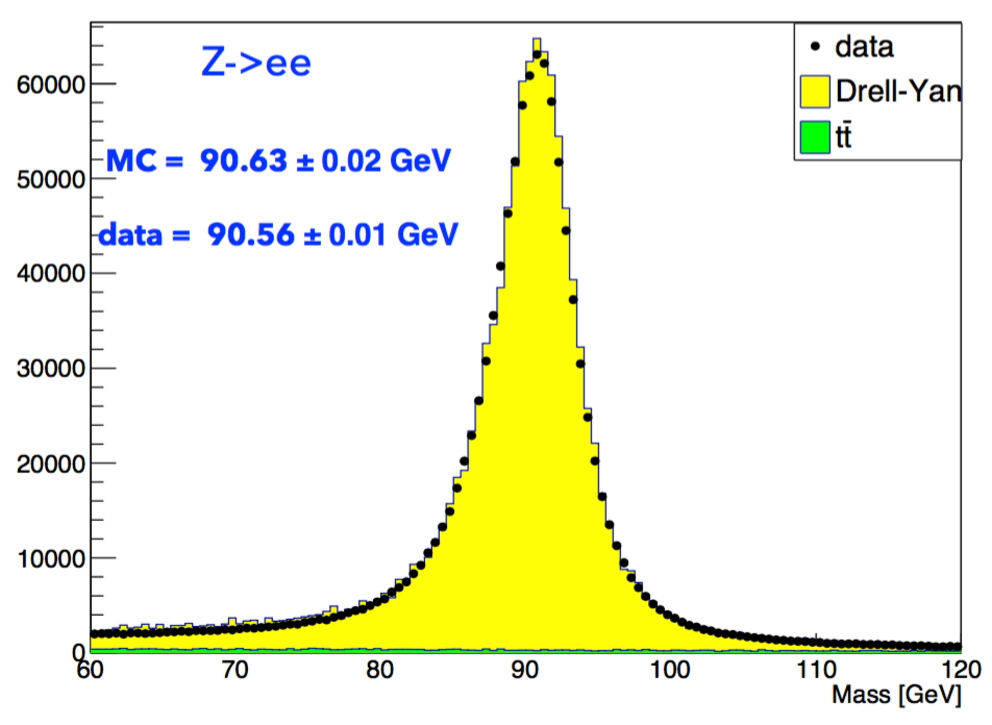
\includegraphics{Figures/Electrons/ele_energy_scale.pdf}}}
%\subfigure [] {\resizebox{9.5cm}{!}{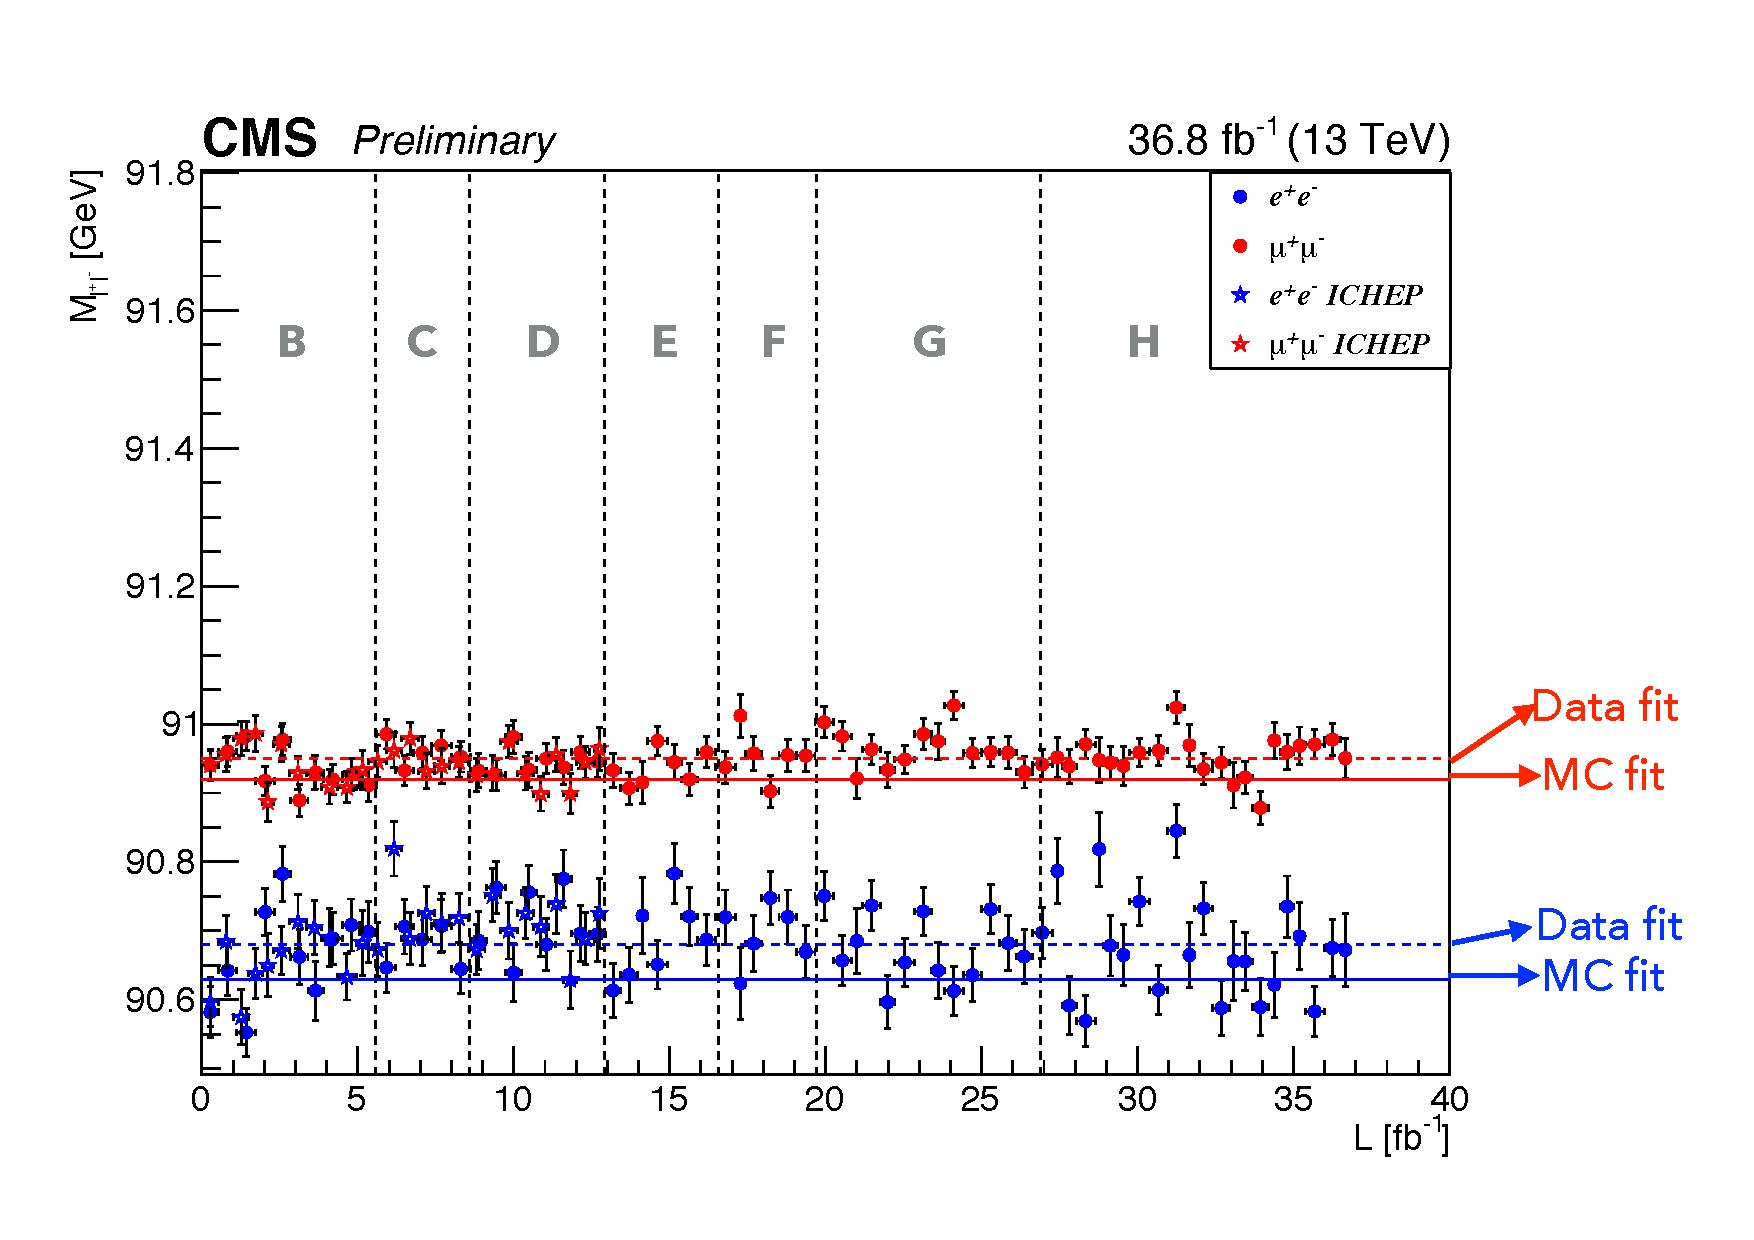
\includegraphics{Figures/Electrons/ele_energy_scale_per_lumi.pdf}}}
%\end{center}
%\caption{
%(a): electron energy scale measured in the $Z+\ell$ control region for EB and EE electrons. The results of the Crystall-ball fit are reported in the figure. 
%(b): lepton energy scales per 500~pb luminosity block. 
%}
%\label{fig:ele_energy_scale}
%\end{figure}

\begin{figure}[tbh]
\centering
\begin{subfigure}{0.45\textwidth}
\centering
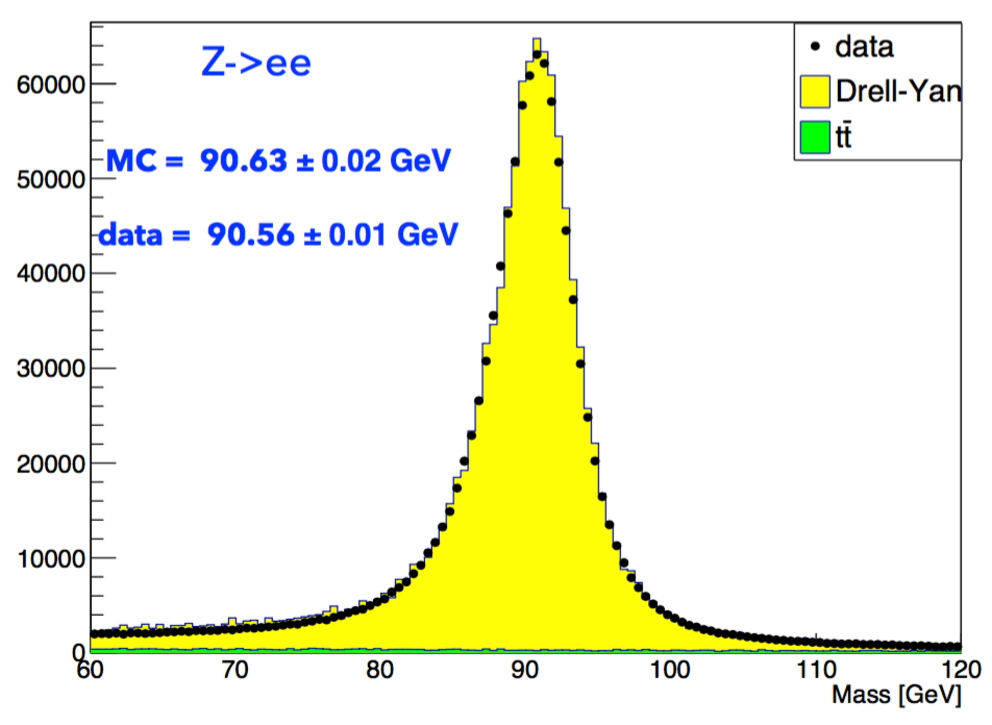
\includegraphics[width=2.5in]{Figures/Electrons/ele_energy_scale.pdf}
\caption{}
\end{subfigure}
\begin{subfigure}{0.45\textwidth}
\centering
\includegraphics[width=2.5in]{Figures/Electrons/ele_energy_scale_per_lumi.pdf}
\caption{}
\end{subfigure}
\caption{(a): electron energy scale measured in the $Z+\ell$ control region for EB and EE electrons. The results of the Crystall-ball fit are reported in the figure. (b): lepton energy scales per 500~pb luminosity block.}
\label{fig:ele_energy_scale}
\end{figure}

\subsection{Electron Efficiency Measurements}
\label{sec:eleEffMeas}
%\input{Objects/eleEffMeas.tex}

The Tag-and-Probe study was performed on the single electron primary datasets listed in table \ref{tab:datasets_data} using the same golden JSON of 36.8 
fb$^{-1}$ as for the main analysis. More details on the Tag-and-Probe method can be found in Ref.~\cite{AN-15-277}. 

Tag electrons need to satisfy the following quality requirements:
\begin{itemize}
\item trigger matched to HLT\_Ele27\_eta2p1\_WPTight\_Gsf\_v*
\item $p_{T} > 30$~GeV, super cluster (SC) $\eta < 2.1$ but on in EB-EE gap ($1.4442<|\eta|<1.566$)
\item tight working point of the Spring16 cut-based electron ID
\end{itemize}

Probe electrons only need to be reconstructed as GsfElectron. The FSR recovery algorithm used in the main analysis is used consistently throughout the efficiency measurement: the isolations are calculated without any FSR photons matched to electrons and the probe electron \pt as well as the di-electron invariant mass include the FSR photons, if any. 


The nominal MC efficiencies are evaluated from the LO MadGraph Drell-Yan sample, while the NLO systematics use the 0,1 jet MadGraph\_AMCatNLO sample listed in Table \ref{tab:MCsamples}.

In contrast to previous efficiency measurements, a template fit is used here. The $m_{ee}$ signal shape of the passing and failing probes is taken from MC and convoluted with a Gaussian. The data is then fitted with the convoluted MC template and a CMSShape (an Error-function with a one-sided exponential tail). This change follows from the usage of the new T\&P tool developed by the EGM POG.


%\paragraph{Electron selection efficiency measurements}\mbox{}\\
%\label{par:Efficiency_measurements}

The electron selection efficiency is measured as a function of the probe electron $\pt$ and its SC $\eta$, and separately for electrons falling in the ECAL gaps. Figure \ref{fig:ele_sel_pt_turn_on} shows the $\pt$ turn-on curves measured in data, and the final 2D scale factor is shown in Fig.~\ref{fig:ele_sel_scale_factors} together with the systematic uncertainties. These scale factors are very similar to the ICHEP figures, but more homogenous across $\eta$ and $\pt$ because of the higher statistics and the usage of more stable fitting routines in the new T\&P tool.


%\begin{figure}[!htb]
%\begin{center}
%    \subfigure [] {\resizebox{7.5cm}{!}{\includegraphics{Figures/Electrons/ele_eff_pt.pdf}}}
%    \subfigure [] {\resizebox{7.5cm}{!}{\includegraphics{Figures/Electrons/gap_ele_eff_pt.pdf}}}\\
%\caption{Electron selection efficiencies measured using the Tag-and-Probe technique described in the text, non-gap electrons (left) and gap electrons (right).}
%\label{fig:ele_sel_pt_turn_on}
%\end{center}
%\end{figure}

\begin{figure}[tbh]
\centering
\begin{subfigure}{0.45\textwidth}
\centering
\includegraphics[width=2.2in]{Figures/Electrons/ele_eff_pt.pdf}
\caption{}
\end{subfigure}
\begin{subfigure}{0.45\textwidth}
\centering
\includegraphics[width=2.2in]{Figures/Electrons/gap_ele_eff_pt.pdf}
\caption{}
\end{subfigure}
\caption{Electron selection efficiencies measured using the Tag-and-Probe technique described in the text, non-gap electrons (left) and gap electrons (right).}
\label{fig:ele_sel_pt_turn_on}
\end{figure}

%\begin{figure}[!htb]
%\begin{center}
%    \subfigure [] {\resizebox{15cm}{!}{\includegraphics{Figures/Electrons/ele_eff_sf_unc.pdf}}}\\
%    \subfigure [] {\resizebox{15cm}{!}{\includegraphics{Figures/Electrons/gap_ele_eff_sf_unc.pdf}}}
%\caption{Electron selection efficiencies measured using the Tag-and-Probe technique described in the text, non-gap electrons (top) and gap electrons (bottom).}
%\label{fig:ele_sel_scale_factors}
%\end{center}
%\end{figure}

\begin{figure}[tbh]
\centering
\begin{subfigure}{0.45\textwidth}
\centering
\includegraphics[width=2.5in]{Figures/Electrons/ele_eff_sf_unc.pdf}
\caption{}
\end{subfigure}
\begin{subfigure}{0.45\textwidth}
\centering
\includegraphics[width=2.5in]{Figures/Electrons/gap_ele_eff_sf_unc.pdf}
\caption{}
\end{subfigure}
\caption{Electron selection efficiencies measured using the Tag-and-Probe technique described in the text, non-gap electrons (top) and gap electrons (bottom)}
\label{fig:ele_sel_scale_factors}
\end{figure}


%\paragraph{Systematic uncertainties}\mbox{}\\
%\label{par:Systematic_uncertainties}
%%%%%%%%%%%%%%%%%%%%%%%%%%%%

 The EGM recommendations on the evaluation of Tag-and-Probe uncertainties for efficiency measurements are followed. Specifically,

\begin{itemize}
   \item Variation of the signal shape from a MC shape to an analytic shape (Crystal Ball) fitted to the MC
   \item Variation of the background shape from a CMS-shape to a simple exponential in fits to data
   \item Variation of the tag selection: tag $p_{T}>$35~GeV and passes MVA-based 8X ID
   \item Using an NLO MC sample for the signal templates
\end{itemize}

The total uncertainty for the measurement of the scale factors is the quadratic sum of the statistical uncertainties returned from the fit and the aforementioned systematic uncertainties.


\section{Muons}

\subsection{Muon Reconstruction and Identification}
\label{sec:muonReco}

More details on muon reconstruction can be found in Ref.~\cite{AN-15-277}.
We define {\bf loose muons} as the muons that satisfy  
$p_T > 5$, $|\eta| < 2.4$, $d_{xy}< 0.5$, $d_z < 1$, where $d_{xy}$ and $d_z$ are 
defined w.r.t. the PV and using the 'muonBestTrack'. Muons have to be 
reconstructed by either the Global Muon or Tracker Muon algorithm. Standalone 
Muon tracks that are only reconstructed in the muon system are rejected.
Muons with \verb|muonBestTrackType==2| (standalone) are discarded even if they 
are marked as global or tracker muons. 

Loose muons with $\pt$ below 200\GeV are considered {\bf tight muons} if they 
also pass the PF muon ID (note that the naming 
convention used for these IDs differs from the muon POG naming scheme, in which
the ``tight ID'' used here is called the ``loose ID''). Loose muons with $\pt$ 
above 200\GeV are considered tight muons if they pass the PF ID or the Tracker
High-$\pt$ ID, the definition of which is shown in Table~\ref{tab:highPtID}.
This relaxed definition is used to increase signal efficiency for the high-mass
search. When a very heavy resonance decays to two $\cPZ$ bosons, both bosons
will be very boosted. In the lab frame, the leptons coming from the decay of
a highly boosted $\cPZ$ will be nearly collinear, and the PF ID loses 
efficiency for muons separated by approximately $\Delta R < 0.4$, which roughly 
corresponds to muons originating from $\cPZ$ bosons with $\pt > 500\GeV$.

\begin{table}[h]
    \begin{small}
    \begin{center}
    \begin{tabular}{|l|l|}
      \hline
      Plain-text description         & Technical description                 \\
      \hline
      Muon station matching          & Muon is matched to segments           \\
                                     & in at least two muon stations         \\
                                     & \textbf{NB: this implies the muon is} \\
                                     & \textbf{an arbitrated tracker muon.}  \\
      \hline                                                          
      Good $\pt$ measurement         & $\frac{\pt}{\sigma_{\pt}} < 0.3$      \\
      \hline
      Vertex compatibility ($x-y$)   & $d_{xy} < 2$~mm                       \\
      \hline
      Vertex compatibility ($z$)     & $d_{z} < 5$~mm                        \\
      \hline
      Pixel hits                     & At least one pixel hit                \\
      \hline
      Tracker hits                   & Hits in at least six tracker layers   \\
      \hline
    \end{tabular}
    \caption{
      The requirements for a muon to pass the Tracker High-$\pt$ ID. Note that
      these are equivalent to the Muon POG High-$\pt$ ID with the global track 
      requirements removed.
      }
    \label{tab:highPtID}
    \end{center}
    \end{small}
\end{table}

An additional ``ghost-cleaning'' step is performed to deal with situations when a single muon
can be incorrectly reconstructed as two or more muons:

\begin{itemize}

\item Tracker Muons that are not Global Muons are required to be arbitrated.
\item If two muons are sharing 50\% or more of their segments then the muon with lower quality is removed.

\end{itemize}

\subsection{Muon Isolation}
\label{sec:muoniso}

Particle-Flow based isolation, described for electrons in section~\ref{sec:eleiso}, is also used for the muons. 
The only difference with electrons is the way the pileup contribution is subtracted: for the muons, $\Delta\beta$ correction is applied, whereby $\Delta\beta = \frac{1}{2} \sum^\text{charged had.}_\text{PU} \pt$  gives an estimate of the energy deposit of neutral particles (hadrons and photons) from pile-up vertices. 
The relative isolation for muons is then defined as:
\begin{equation}
\text{RelPFiso} = \frac{\sum^\text{charged had.} \pt + \max(\sum^\text{neutral had.} \ET 
+ \sum^\text{photon} \ET - \Delta \beta, 0)}{\pt^\text{lepton}}
\label{eqn:mupfiso}
\end{equation}

The isolation working point for muons was optimized in Ref.~\cite{AN-15-277} and the working point was chosen to be the same as electrons,
namely $\text{RelPFiso}(\Delta R = 0.3) < 0.35$. 


%\subsection{Muon Energy Calibrations}
% \input{Objects/muCalib}

\subsection{Muon Efficiency Measurements}
\label{sec:muonEffMeas}

Muon efficiencies are measured with the Tag and Probe (T\&P) method performed on
$\cPZ \to \Pgm\Pgm$ and $\JPsi\to\mu\mu$ events in bins of $\pt$ and $\eta$. More
details on the methodology can be found in Ref.~\cite{AN-15-277}.
%
The $\Z$ sample is used to measure the muon reconstruction and identification efficiency at high $\pt$,
and the efficiency of the isolation and impact parameter requirements at all $\pt$.
%
The $\JPsi$ sample is used to measure the reconstruction efficiency at low $\pt$,
as it benefits from a better purity in that kinematic regime. In this case,
events are collected using \verb=HLT_Mu7p5_Track2_Jpsi_v*= when probing the
reconstruction and identification efficiency in the muon system, and using the
 \verb=HLT_Mu7p5_L2Mu2_Jpsi_v*= when probing the tracking efficiency.

\paragraph*{Reconstruction and identification}

Results for the muon reconstruction and identification efficiency for $\pt > 20\GeV$
have been derived by the Muon POG.
The probe in this measurement are tracks reconstructed in the inner tracker, and
the passing probes are those that are also reconstructed as a global or tracker muon 
and passing the Muon POG Loose muon identification.
%
Results for low $\pt$ muons were derived using \JPsi events, with the same definitions
of probe and passing probes. The systematic uncertainties are estimated by varying the analytical signal and background shape models used to fit 
the dimuon invariant mass. Details on the procedure can be found in Ref.~\cite{AN-15-277}. The efficiency and scale 
factors used for low $\pt$ muons are the ones derived using single muon prompt-reco dataset.

The efficiency in data and simulation is shown in Fig.~\ref{fig:MuonIDEff_1}. 


\begin{figure}[tbh]
\centering
\begin{subfigure}{0.25\textwidth}
\centering
\includegraphics[width=1.5in]{Figures/Muons/mu_Loose_barrel.pdf}
\caption{}
\end{subfigure}
\begin{subfigure}{0.25\textwidth}
\centering
\includegraphics[width=1.5in]{Figures/Muons/mu_Loose_endcap.pdf}
\caption{}
\end{subfigure}
\begin{subfigure}{0.25\textwidth}
\centering
\includegraphics[width=1.5in]{Figures/Muons/mu_Loose_pt7.pdf}
\caption{}
\end{subfigure}
    \caption{Muon reconstruction and identification efficiency at low \pt, measured with the tag\&probe method on \JPsi events, as function of \pt in the barrel (left) and endcaps (center), and as function of $\eta$ for $\pt > 7\GeV$ (right). In the upper panel, the larger error bars include also the systematical uncertainties, while the smaller ones are purely statistical. In the lower panel showing the ratio of the two efficiencies, the black error bars are for the statistical uncertainty, the orange rectangles for the systematical uncertainty and the violet rectangles include both uncertainties.}
\label{fig:MuonIDEff_1}
\end{figure}

%\begin{figure}[htbp]
%  \begin{center}
%    \subfigure[]{\includegraphics[width=0.32\textwidth]{Figures/Muons/mu_Loose_barrel.pdf}}
%    \subfigure[]{\includegraphics[width=0.32\textwidth]{Figures/Muons/mu_Loose_endcap.pdf}}
%    \subfigure[]{\includegraphics[width=0.32\textwidth]{Figures/Muons/mu_Loose_pt7.pdf}}
%    \caption{Muon reconstruction and identification efficiency at low \pt, measured with the tag\&probe method on \JPsi events, as function of \pt in the barrel (left) and endcaps (center), and as function of $\eta$ for $\pt > 7\GeV$ (right). In the upper panel, the larger error bars include also the systematical uncertainties, while the smaller ones are purely statistical. In the lower panel showing the ratio of the two efficiencies, the black error bars are for the statistical uncertainty, the orange rectangles for the systematical uncertainty and the violet rectangles include both uncertainties.}
%    \label{fig:MuonIDEff_1}
%\end{center}
%\end{figure}

\paragraph*{Impact parameter requirements}
The measurement is performed using $\Z$ events. Events are selected with \verb=HLT_IsoMu20_v*= or \verb=HLT_IsoMu22_v*= triggers.
For this measurement, the probe is a muon passing the POG Loose identification criteria,
and it is considered a passing probe if satisfies the SIP3D, dxy, dz cuts of this analysis.
%
The results are shown in Fig.~\ref{fig:MuonIDEff_2}.
%Very good agreement between data and simulation is observed in the barrel (Fig.~\ref{fig:MuonIDEff_2}, left)
%while some inefficiency is visible in the endcaps, especially at large values of $|\eta|$.
%The data to simulation scale factor is found to be flat as function of \pt, so, similarly to what done
%for the identification part, we apply a correction only as function of $\eta$.


\begin{figure}[tbh]
\centering
\begin{subfigure}{0.25\textwidth}
\centering
\includegraphics[width=1.5in]{Figures/Muons/mu_SIP4_barrel.pdf}
\caption{}
\end{subfigure}
\begin{subfigure}{0.25\textwidth}
\centering
\includegraphics[width=1.5in]{Figures/Muons/mu_SIP4_endcap.pdf}
\caption{}
\end{subfigure}
\begin{subfigure}{0.25\textwidth}
\centering
\includegraphics[width=1.5in]{Figures/Muons/mu_SIP4_pt20.pdf}
\caption{}
\end{subfigure}
\caption{Efficiency of the muon impact parameter requirements, measured with the tag\&probe method on \Z events, as function of \pt in the barrel (left) and endcaps (center), and as function of $\eta$ for $\pt > 20\GeV$ (right). In the upper panel, the larger error bars include also the systematical uncertainties, while the smaller ones are purely statistical. In the lower panel showing the ratio of the two efficiencies, the black error bars are for the statistical uncertainty, the orange rectangles for the systematical uncertainty and the violet rectangles include both uncertainties.}
\label{fig:MuonIDEff_2}
\end{figure}

%\begin{figure}[htbp]
%  \begin{center}
%    \subfigure[]{\includegraphics[width=0.32\textwidth]{Figures/Muons/mu_SIP4_barrel.pdf}}
%    \subfigure[]{\includegraphics[width=0.32\textwidth]{Figures/Muons/mu_SIP4_endcap.pdf}}
%    \subfigure[]{\includegraphics[width=0.32\textwidth]{Figures/Muons/mu_SIP4_pt20.pdf}}
%    \caption{Efficiency of the muon impact parameter requirements, measured with the tag\&probe method on \Z events, as function of \pt in the barrel (left) and endcaps (center), and as function of $\eta$ for $\pt > 20\GeV$ (right). In the upper panel, the larger error bars include also the systematical uncertainties, while the smaller ones are purely statistical. In the lower panel showing the ratio of the two efficiencies, the black error bars are for the statistical uncertainty, the orange rectangles for the systematical uncertainty and the violet rectangles include both uncertainties.}
%    \label{fig:MuonIDEff_2}
%\end{center}
%\end{figure}

\paragraph*{Isolation requirements}
The isolation efficiency is measured using events from the $\Z$ decay for any \pt, selected with either of \verb=HLT_IsoMu20_v*= or \verb=HLT_IsoMu22_v*= triggers. The isolation of the muons are calculated after recovery of the FSR photons and subtracting their contribution to the isolation cone of the muons. More detailed description of the method can be found in Ref.~\cite{AN-16-217}.

The results are shown in Fig.~\ref{fig:MuonIDEff_3}.

\begin{figure}[tbh]
\centering
\begin{subfigure}{0.45\textwidth}
\centering
\includegraphics[width=2.5in]{Figures/Muons/mu_iso_barrel.pdf}
\caption{}
\end{subfigure}
\begin{subfigure}{0.45\textwidth}
\centering
\includegraphics[width=2.5in]{Figures/Muons/mu_iso_endcap.pdf}
\caption{}
\end{subfigure}
    \caption{Efficiency of the muon isolation requirement, measured with the tag\&probe method on \Z events, as function of \pt in the barrel (left) and endcaps (right). In the upper panel, the larger error bars include also the systematical uncertainties, while the smaller ones are purely statistical. In the lower panel showing the ratio of the two efficiencies, the black error bars are for the statistical uncertainty, the orange rectangles for the systematical uncertainty and the violet rectangles include both uncertainties.}
\label{fig:MuonIDEff_3}
\end{figure}

%\begin{figure}[htbp]
%  \begin{center}
%    \subfigure[]{\includegraphics[width=0.32\textwidth]{Figures/Muons/mu_iso_barrel.pdf}}
%    \subfigure[]{\includegraphics[width=0.32\textwidth]{Figures/Muons/mu_iso_endcap.pdf}}
%    \caption{Efficiency of the muon isolation requirement, measured with the tag\&probe method on \Z events, as function of \pt in the barrel (left) and endcaps (right). In the upper panel, the larger error bars include also the systematical uncertainties, while the smaller ones are purely statistical. In the lower panel showing the ratio of the two efficiencies, the black error bars are for the statistical uncertainty, the orange rectangles for the systematical uncertainty and the violet rectangles include both uncertainties.}
%    \label{fig:MuonIDEff_3}
%\end{center}
%\end{figure}

\paragraph*{Tracking}
The efficiency to reconstruct a muon track in the inner detector is measured using as probes tracks
reconstructed in the muon system alone. The method for measuring the tracking efficiency is the same as 
 in Ref.~\cite{CMS_AN_2015-215}, and the results on 2016 data are briefly discussed here. The efficiency and 
data to mc scale factors are measured from Z events as a function of $\eta$ for $\pt > 10\GeV$ and $\pt < 10\GeV$. The values of data to mc scale factors 
used are from the ReReco version of the full dataset collected in 2016. 

The tracking efficiency in data and simulation as a function of $\eta$ is shown in Fig.~\ref{fig:MuonIDEff_4}.

\begin{figure}[tbh]
\centering
\begin{subfigure}{0.45\textwidth}
\centering
\includegraphics[width=2.5in]{Figures/Muons/trackingEffptl10.pdf}
\caption{}
\end{subfigure}
\begin{subfigure}{0.45\textwidth}
\centering
\includegraphics[width=2.5in]{Figures/Muons/trackingEffptg10.pdf}
\caption{}
\end{subfigure}
    \caption{Tracking efficiency in data and simulation as a function of $\eta$ for muon $\pt < 10\GeV$(left) and $\pt > 10\GeV$(right) with ReReco data.}
    \label{fig:MuonIDEff_4}
\end{figure}

%\begin{figure}[htbp]
%  \begin{center}
%    \subfigure[]{\includegraphics[width=0.42\textwidth]{Figures/Muons/trackingEffptl10.pdf}}
%    \subfigure[]{\includegraphics[width=0.42\textwidth]{Figures/Muons/trackingEffptg10.pdf}}
%    \caption{Tracking efficiency in data and simulation as a function of $\eta$ for muon $\pt < 10\GeV$(left) and $\pt > 10\GeV$(right) with ReReco data.}
%    \label{fig:MuonIDEff_4}
%\end{center}
%\end{figure}

\paragraph*{Overall results}
The product of all the data to simulation scale factors for muon tracking, reconstruction, identification, impact parameter and isolation requirements is shown in Fig.~\ref{fig:MuonIDEff_5}. 
%The overall correction is about $-1\%$ or less for most \pt and $\eta$ values, increasing to about $-2\%$ in for muons below $10\GeV$ or with $|\eta|>2$.

\begin{figure}[tbh]
\centering
\begin{subfigure}{0.45\textwidth}
\centering
\includegraphics[width=2.5in]{Figures/Muons/mu_sf.pdf}
\caption{}
\end{subfigure}
\begin{subfigure}{0.45\textwidth}
\centering
\includegraphics[width=2.5in]{Figures/Muons/mu_sf_unc.pdf}
\caption{}
\end{subfigure}
    \caption{Left: Overall data to simulation scale factors for muons, as function of \pt and $\eta$. Right: Uncertainties on  data to simulation scale factors for muons, as function of \pt and $\eta$.}
    \label{fig:MuonIDEff_5}
\end{figure}

%\begin{figure}[htbp]
%  \begin{center}
%    \includegraphics[width=0.45\textwidth]{Figures/Muons/mu_sf.pdf}
%    \includegraphics[width=0.45\textwidth]{Figures/Muons/mu_sf_unc.pdf}
%    \caption{Left: Overall data to simulation scale factors for muons, as function of \pt and $\eta$. Right: Uncertainties on  data to simulation scale factors for muons, as function of \pt and $\eta$.}
%    \label{fig:MuonIDEff_5}
%\end{center}
%\end{figure}


\section{Photons for FSR recovery}
\label{sec:FSRphotons}

The FSR recovery algorithm was considerably simplified with respect to what was done in Run I, while maintaining similar performance. 
The selection of FSR photons is now only done per-lepton and no longer depends on any Z mass criterion, thus much simplifying the subsequent ZZ candidate building and selection. As regards the association of photons with leptons, the rectangular cuts on $\Delta R(\gamma,l)$ and $E_{T,\gamma}$  have been replaced by a cut on $\Delta R(\gamma,l)/E_{T,\gamma}^{2}$.

Starting from the collection of 'PF photons' provided by the particle-flow algorithm, the selection of photons and their association to a lepton proceeds as follows:
\begin{enumerate}
\item The preselection of PF photons is done by requiring $p_{T,\gamma} > 2~\GeV$, $|\eta^{\gamma}| < 2.4$, and a relative Particle-flow isolation smaller than $1.8$. The latter variable is computed using a cone of radius $R=0.3$, a threshold of $0.2~\GeV$ on charged hadrons with a veto cone of $0.0001$, and $0.5~\GeV$ on neutral hadrons and photons with a veto cone of $0.01$, also including the contribution from pileup vertices (with the same radius and threshold as per charged isolation) .
\item Supercluster veto: we remove all PF photons that match with any electron passing both the loose ID and SIP cuts. The matching is peformed by directly associating the two PF candidates.
\item Photons are associated to the closest lepton in the event among all those pass both the loose ID and SIP cuts.
\item We discard photons that fail the cuts $\Delta R(\gamma,l)/E_{T,\gamma}^2 < 0.012$, and $\Delta R(\gamma,l)<0.5$.
\item If more than one photon is associated to the same lepton, the lowest-$\Delta R(\gamma,l)/E_{T,\gamma}^2$ is selected.
\item For each FSR photon that was selected, we exclude that photon from the isolation sum of all the leptons in the event that pass both the loose ID and SIP cuts. This concerns the photons that are in the isolation cone and outside the isolation veto of said leptons ($\Delta R < 0.4$ AND $\Delta R > 0.01$ for muons and $\Delta R < 0.4$ AND ($\eta^{\text{SC}} < 1.479$ OR $\Delta R > 0.08$) for electrons).
\end{enumerate}

More details on the optimization of the FSR photon selection can be found in Ref.~\cite{AN-15-277, AN-16-217}.

\section{Jets}
\label{sec:jets}

Vector Boson Fusion (VBF) and other production mechanisms of Higgs Boson normally differ as regards the jet kinematics. 
In this analysis, jets are thus used for the event categorization, which will be introduced in Section~\ref{sec:categorization}.

\subsubsection{Jet Identification}

Jets are reconstructed by using the anti-$k_T$ clustering algorithm out of particle flow candidates, with a distance parameter $R = 0.4$, 
after rejecting the charged hadrons that are associated to a pileup primary  vertex.

To reduce instrumental background, the loose working point jet ID suggested by the JetMET Physics Object Group is applied. 
In this analysis, the jets are required to be within $|\eta| < 4.7$ area and have a transverse momentum above 30 GeV. 
In addition, the jets are cleaned from any of the tight leptons (passing the SIP and isolation cut computed after FSR correction) 
and FSR photons by a separation criterion: $\Delta R(\text{jet,lepton/photon}) > 0.4$.


\subsubsection{Jet Energy Corrections}

The calorimeter response to particles is not linear
and it is not straightforward to translate the measured jet energy
to the true particle or parton energy, therefore we need Jet Energy Corrections.
In this analysis, standard jet energy corrections are applied to the reconstructed jets,
which consist of L1 Pileup, L2 Relative Jet Correction,
L3 Absolute Jet Correction for both Monte Carlo samples and data,
and also residual calibration for data.

% Figure~\ref{fig:jets} shows the comparisoin between data and MC for the leading jet in Z events with exactly one jet,
% where a selection $\Delta\phi(Z,{\rm jet})>2.5$ has been applied.

% \begin{figure}[!h]
% \centering
% \includegraphics[width=0.49\linewidth]{Figures/Jets/Histo_etaj1_2e_dataeff.pdf}
% \includegraphics[width=0.49\linewidth]{Figures/Jets/Histo_etaj1_2mu_dataeff.pdf}
% \caption{Comparison between data and MC for jet $\eta$ in Z + 1 jet events. \label{fig:jets}}
% \end{figure}


\subsubsection{B-tagging}

For categorization purpose, we need to distinguish whether a jet is b-jet or not.
The \emph{Combined Secondary Vertex} algorithm is used as our b-tagging algorithm.
It combines information about impact parameter significance,
the secondary vertex and jet kinematics.
The variables are combined using a likelihood ratio technique to compute the b-tag discriminator.
In this analysis, a jet is considered to be b-tagged if it passes the \emph{CSVv2M} working point,
i.e. if its \verb|pfCombinedInclusiveSecondaryVertexV2BJetTags| discriminator is greater than 0.8484~\cite{btagReferenceEffsRun2}.

Data to simulation scale factors for b-tagging efficiency are provided for this working point for the full dataset as a function of jet $\pt$, $\eta$ and flavour.
They are applied to simulated jets by downgrading (upgrading) the b-tagging status of a fraction of the b-tagged (untagged) jets that have a scale factor smaller (larger) than one.

\section{MET}

The missing transverse energy, $E_{\rm{T}}^{\rm{MISS}}$ or MET, of an event is defined as the magnitude of the imbalance of momentum in the plane transverse to the beam line. Since momentum is conserved in this plane, any imbalance in momentum is attributed to particles escaping the detector without interacting with the detector material, such as neutrinos or hypothetical dark matter candidates. Raw MET or particle flow MET (PFMET) is defined as the magnitude of the negative vectorial sum of the transverse momentum of all reconstructed particle flow candidates, or

\begin{equation}
\overrightarrow{E}_{\rm{T}}^{\rm{MISS}} = - \sum_{i \in \rm{all}} \overrightarrow{p}_{\rm{T},\ i}
\end{equation}

The vector quantity that is the negative sum of reconstructed particle momenta is sometimes called the missing transverse momentum, although this term is used interchangably with its magnitude, the MET. 

An alternative definition of the MET, called the type-I corrected MET, takes into account the jet energy corrections (JEC), correcting for mismeasurment of MET due to detector inefficiencies and non linear responses in the calorimeters. The type-I corrected MET definition is given in Equation~\ref{eq:t1met}. Systematic uncertainties related to modelling real MET are obtained by varying the JEC and jet energy resolution (JER) and measuring the propogation of these variations to the MET uncertainty. These measurements are described in greater detail in the next section.

\begin{equation}
\label{eq:t1met}
\overrightarrow{E}_{\rm{T\ Type-I}}^{\rm{MISS}} = - \sum_{jet} \overrightarrow{p}_{\rm{T},\ jet}^{\rm{JEC}} - \sum_{i \in \rm{uncl.}} \overrightarrow{p}_{\rm{T},\ i}
\end{equation}

where the total contribution has been split into contributions from jets (first term) and contributions from unclustered objects (second term). The transverse momenta of jets in the first term is then replaced with the JEC transverse momenta.

\subsubsection{MET filters}

Due to detector and instrumental noise, several filters are applied to veto noisy events \cite{mettwiki}:

\begin{itemize}
\item HBHENoiseFilter
\item HBHENoiseIsoFilter 
\item EcalDeadCellTriggerPrimitiveFilter 
\item goodVertices 
\item eeBadScFilter 
\item globalTightHalo2016Filter 
\item BadPFMuonFilter 
\item BadChargedCandidateFilter
\end{itemize}

The first two filters remove noisy events from the HCAL, where the HBHE scintillator produce anamolous signals with pulse shapes and pixel multiplicities discrepant from those from a clean signal. The EcalDeadCellTriggerPrimitiveFilter removes events with down ECAL data links, comparing the sum of energy deposited in each cell of a supercluster to the trigger primitive saturation energy. goodVertices removes events with noisy vertex reconstruction from pileup effects. The eeBadScFilter removes events with noisy ECAL end cap super clusters. globalTightHalo2016Filter removes events with enhanced MET from beam-halo particles which are in time with the beam. The last two filters remove events with mis-reconstructed muon and charged hadron particle flow candidates.

\subsubsection{Fake MET modeling}\label{sec:fakemet}

Figure~\ref{fig:pfmet_m4lblinded} shows a discrepancy between data and MC in the high-$E_{\rm{T}}^{\rm{MISS}}$ tail. These events typically contain a high $p_T$ object either back-to-back or collinear with the $E_{\rm{T}}^{\rm{MISS}}$, pointing to artificially high $E_{\rm{T}}^{\rm{MISS}}$ from mismeasurement of the object. These fake events are identified and removed by studying distributions of the transverse angular difference between the MET and various objects in the event \cite{CMS-AN-15-203}.

\begin{figure}[tbh]
\centering
\includegraphics[width=5in]{figures/hist_hPFMET_8.png}
\caption{Missing transverse energy after SM selection before removal of fake MET.}
\label{fig:pfmet_m4lblinded}
\end{figure}

Several variables are studied in order to understand how to remove these fake events from data:

\begin{itemize}
  \item $max|\Delta\phi(jet, E_{\rm{T}}^{\rm{MISS}})|$ with the maximum taken over selected jets, Figure~\ref{fig:maxdeltaphijmet}
  \item $min|\Delta\phi(jet, E_{\rm{T}}^{\rm{MISS}})|$ with the minimum taken over selected jets, Figure~\ref{fig:mindeltaphijmet}
\end{itemize}

The max variables are to check for the occurance of objects with mismeasured energy back-to-back with the MET, the min variable is to check for jets with mismeasured energy collinear with the MET.

\begin{figure}[tbh]
\centering
\includegraphics[width=5in]{figures/hist_hDPHI_MAX_JET_MET_8.png}
\caption{Maximum azimuthal angle difference between MET and jets.}
\label{fig:maxdeltaphijmet}
\end{figure}

\begin{figure}[tbh]
\centering
\includegraphics[width=5in]{figures/hist_hDPHI_MIN_JET_MET_8.png}
\caption{Minimum azimuthal angle difference between MET and jets.}
\label{fig:mindeltaphijmet}
\end{figure}

For jets with a high transverse momentum, greater than 50 GeV, it is required that $max|\Delta\phi(jet, E_{\rm{T}}^{\rm{MISS}})|<2.7$ and $min|\Delta\phi(jet, E_{\rm{T}}^{\rm{MISS}})|>0.5$ to exclude events with large MET from mismeasurment of jet energies. These cuts are based on the Run 1 SM analysis selection, chosen to balance the small loss in signal efficiency with the increased systematic uncertainty from mismodelling of the MET in background MC simulations (described in Section~\ref{sec:metsyst}).


\chapter{Signal and control regions}

\section{Event selection}

\subsection{Trigger selection}
\label{sec:HLTsel}

The events are required to have fired the High-Level Trigger (HLT) paths described in section~\ref{sec:trigpaths}. Unlike in the Run 1 analysis, the trigger requirement in the Run 2 analysis does not depend on the selected final state. Instead, it is always the OR of all ten HLT paths, since associated production modes that can have additional leptons will be targeted. This improves the trigger efficiency further.

\subsection{Vertex selection}
\label{sec:vertexsel}

The events are required to have at least one good primary
vertex (PV) fullfilling all three of the following criteria: a high number of degrees
of freedom ($N_{PV}>4$), collisions restricted along the $z$-axis
($z_{PV}<24$ cm), and a small radius of the PV ($r_{PV}<2$ cm).


\subsection{$ZZ$ candidate selection}
\label{sec:zzcandsel}

The four-lepton candidates are built from ``selected'' leptons, which  
are the tight leptons (defined in Sections~\ref{sec:eleID} and~\ref{sec:muonReco}) that pass the ${\rm SIP_{3D}} < 4$ vertex constraint
and the isolation cuts (defined in Sections~\ref{sec:eleiso} and~\ref{sec:muoniso}), 
where FSR photons are subtracted as described in Section~\ref{sec:FSRphotons}. The muon isolation and SIP distributions are shown in Figure~\ref{fig:lepkin1}.
A lepton cross-cleaning is applied 
by discarding electrons that are within $\Delta R < 0.05$ of selected muons. Additional kinematics for these leptons at the stage they are selected are shown in Figure~\ref{fig:lepkin2}.

 
\begin{figure}[tbh]
\begin{subfigure}{0.50\textwidth}
\centering
\includegraphics[width=3.3in]{figures/hist_hPtLep_3.png}
\caption{}
\end{subfigure}
\begin{subfigure}{0.50\textwidth}
\centering
\includegraphics[width=3.3in]{figures/hist_hEtaLep_3.png}
\caption{}
\end{subfigure}
\caption{Selected lepton kinematics: (a) transverse momentum and (b) $\eta$.}
\label{fig:lepkin1}
\end{figure}
 
\begin{figure}[tbh]
\begin{subfigure}{0.50\textwidth}
\centering
\includegraphics[width=3.3in]{figures/hist_hIsoLep_3.png}
\caption{}
\end{subfigure}
\begin{subfigure}{0.50\textwidth}
\centering
\includegraphics[width=3.3in]{figures/hist_hSipLep_3.png}
\caption{}
\end{subfigure}
\caption{Selected lepton kinematics: (a) lepton isolation and (b) SIP vertex constraint.}
\label{fig:lepkin2}
\end{figure}

 

The construction and selection of four-lepton candidates proceeds 
according to the following sequence:
\begin{enumerate}
\item {\bf $Z$ candidates} are defined as pairs of selected leptons
 of opposite charge and matching flavor (e.g. $e^+ e^-$ or $\mu^+\mu^-$)
 that satisfy $12 < m_{\ell\ell(\gamma)} < 120~\GeV$, where the $Z$ candidate mass
 includes the selected FSR photons if any. The dimuon invariant mass distribution for $Z$ candidates at this step is shown in Figure~\ref{fig:dimuonz}. The distribution of $\MET$ at this step, showing a large contribution from $Z+X$, is shown in Figure~\ref{fig:pfmet3}.

\begin{figure}[tbh]
\centering
\includegraphics[width=5.5in]{figures/hist_hMZ_3.png}
    \caption{Dimuon invariant mass distribution for $Z$ candidates.}
    \label{fig:dimuonz}
\end{figure}

\begin{figure}[tbh]
\centering
\includegraphics[width=5.5in]{figures/hist_hPFMET_3.png}
    \caption{Missing transverse energy distribution at the $Z$ candidate selection step.}
    \label{fig:pfmet3}
\end{figure}

\item {\bf $ZZ$ candidates} are defined as pairs of non-overlapping $Z$ candidates.
 The $Z$ candidate with reconstructed mass $m_{\ell\ell}$ closest to the nominal $Z$ boson
 mass is denoted as $\Z_1$, and the second one is denoted as $Z_2$. The dimuon distributions for $Z_1$ and $Z_2$ at this step are shown in Figure~\ref{fig:dimuonz5}. Additional kinematics for the $Z_1$ and $Z_2$ candidates are shown in Figures~\ref{fig:z15kin} and \ref{fig:z25kin}. Kinematics for the constituent muons are shown in Figures~\ref{fig:lep5kin1} and \ref{fig:lep5kin2}.

\begin{figure}[tbh]
\begin{subfigure}{0.50\textwidth}
\centering
\includegraphics[width=3.3in]{figures/hist_hMZ1_5.png}
\caption{}
\end{subfigure}
\begin{subfigure}{0.50\textwidth}
\centering
\includegraphics[width=3.3in]{figures/hist_hMZ2_5.png}
\caption{}
\end{subfigure}
\caption{Dimuon invariant mass at the $ZZ$ candidate selection step for (a) $Z_1$ and (b) $Z_2$.}
\label{fig:dimuonz5}
\end{figure}

\begin{figure}[tbh]
\begin{subfigure}{0.50\textwidth}
\centering
\includegraphics[width=3.3in]{figures/hist_hPtZ1_5.png}
\caption{}
\end{subfigure}
\begin{subfigure}{0.50\textwidth}
\centering
\includegraphics[width=3.3in]{figures/hist_hYZ1_5.png}
\caption{}
\end{subfigure}
\caption{Kinematic distributions for the $Z_1$ at the $ZZ$ candidate selection step: (a) $\pt$ and (b) $\eta$.}
\label{fig:z15kin}
\end{figure}

\begin{figure}[tbh]
\begin{subfigure}{0.50\textwidth}
\centering
\includegraphics[width=3.3in]{figures/hist_hPtZ2_5.png}
\caption{}
\end{subfigure}
\begin{subfigure}{0.50\textwidth}
\centering
\includegraphics[width=3.3in]{figures/hist_hYZ2_5.png}
\caption{}
\end{subfigure}
\caption{Kinematic distributions for the $Z_2$ at the $ZZ$ candidate selection step: (a) $\pt$ and (b) $\eta$.}
\label{fig:z25kin}
\end{figure}

\begin{figure}[tbh]
\begin{subfigure}{0.50\textwidth}
\centering
\includegraphics[width=3.3in]{figures/hist_hPtLep1_5.png}
\caption{}
\end{subfigure}
\begin{subfigure}{0.50\textwidth}
\centering
\includegraphics[width=3.3in]{figures/hist_hPtLep2_5.png}
\caption{}
\end{subfigure}
\begin{subfigure}{0.50\textwidth}
\centering
\includegraphics[width=3.3in]{figures/hist_hPtLep3_5.png}
\caption{}
\end{subfigure}
\begin{subfigure}{0.50\textwidth}
\centering
\includegraphics[width=3.3in]{figures/hist_hPtLep4_5.png}
\caption{}
\end{subfigure}
\caption{Transverse momentum distributions for the constituent leptons of the $Z_1$, (a) and (b), and of the $Z_2$, (c) and (d) at the $ZZ$ candidate selection step.}
\label{fig:lep5kin1}
\end{figure}

\begin{figure}[tbh]
\begin{subfigure}{0.50\textwidth}
\centering
\includegraphics[width=3.3in]{figures/hist_hEtaLep1_5.png}
\caption{}
\end{subfigure}
\begin{subfigure}{0.50\textwidth}
\centering
\includegraphics[width=3.3in]{figures/hist_hEtaLep2_5.png}
\caption{}
\end{subfigure}
\begin{subfigure}{0.50\textwidth}
\centering
\includegraphics[width=3.3in]{figures/hist_hEtaLep3_5.png}
\caption{}
\end{subfigure}
\begin{subfigure}{0.50\textwidth}
\centering
\includegraphics[width=3.3in]{figures/hist_hEtaLep4_5.png}
\caption{}
\end{subfigure}
\caption{$\eta$ distributions for the constituent leptons of the $Z_1$, (a) and (b), and of the $Z_2$, (c) and (d) at the $ZZ$ candidate selection step.}
\label{fig:lep5kin2}
\end{figure}


$ZZ$ candidates are required to satisfy the following list of requirements:
  \begin{itemize} 
  \item {\bf Ghost removal }: $\Delta R(\eta,\phi) > 0.02$ between each of the four leptons
  \item {\bf Lepton $p_T$}: two of the four selected leptons should pass 
     $p_{T,i} > 20~\GeV$ and $p_{T,j} > 10~\GeV$
  \item {\bf QCD suppression}: all four oppositely-signed pairs that can
     be built with the four leptons (regardless of lepton flavor)
     must satisfy $m_{\ell\ell} > 4~\GeV$.
     Here, selected FSR photons are not used in computing $m_{\ell\ell}$, 
     since a QCD-induced low-mass dilepton (e.g. $J/\Psi$) 
     may have photons nearby (e.g. from $\pi_0$)
  \item {\bf $Z_1$ mass}: $m_{Z1} > 40~\GeV$
  \item {\bf `smart cut'}: defining $Z_a$ and $Z_b$ as 
     the mass-sorted alternative pairing $Z$ candidates 
     ($Z_a$ being the one closest to the nominal $Z$ boson mass),
     require NOT($|m_{ Za}-m_{ Z}| < |m_{ Z1}-m_{ Z}|$ AND $m_{ Zb}<12$).
     Selected FSR photons are included in $m_{ Z}$'s computations.
     This cut discards $4\mu$ and $4e$ candidates where the alternative pairing
     looks like an on-shell $Z$ + low-mass $\ell^+ \ell^-$. 
     In Run 1, such a situation was avoided by choosing the best $ZZ$ candidate
     before applying kinematic cuts to it, most precisely before the $m_{Z2} > 12~\GeV$ cut.
     The present smart cut allows to choose the best $ZZ$ candidate after all kinematic cuts.
The four-lepton invariant mass for the $ZZ$ candidates at this stage is shown in Figure~\ref{fig:m4mu5}.   

\begin{figure}[tbh]
\centering
\includegraphics[width=5.5in]{figures/hist_hM4l_5_log.png}
    \caption{Four-muon invariant mass distribution at the $ZZ$ selection step in log scale.}
    \label{fig:m4mu5}
\end{figure}

  \item {\bf Four-lepton invariant mass}: $\mllll > 70~\GeV$. 
%The four-muon invariant mass distribution after all of the previous selection steps are applied is shown in Figure~\ref{fig:m4mu}(a), with a close up view of the $Z$ and $H$ peaks shown in Figure~\ref{fig:m4mu}(b). 
Additional kinematics for the $4l$ object are shown in Figure~\ref{fig:4mukin}. The kinematics of the $Z_1$ and $Z_2$ candidates used in the final SM selection are shown in Figure~\ref{fig:dimuonzmass} with the constituent lepton kinematics shown in Figures~\ref{fig:leptkinsm1}, \ref{fig:leptkinsm2}, and \ref{fig:leptkinsm3}. Finally, the MET distribution at this step is shown in Figure~\ref{fig:met8}
  \end{itemize}	
\item Events containing at least one selected $ZZ$ candidate form the SM signal region.
\end{enumerate}	

\begin{figure}[tbh]
\begin{subfigure}{0.50\textwidth}
\centering
\includegraphics[width=3.3in]{figures/hist_hpt4l_CR.png}
\caption{}
\end{subfigure}
\begin{subfigure}{0.50\textwidth}
\centering
\includegraphics[width=3.3in]{figures/hist_heta4l_CR.png}
\caption{}
\end{subfigure}
\caption{Kinematics of the four-muon object after the final SM selection: (a) transverse momentum and (b) $\eta$.}
\label{fig:4mukin}
\end{figure}

\begin{figure}[tbh]
\begin{subfigure}{0.50\textwidth}
\centering
\includegraphics[width=3.3in]{figures/hist_hZ1mass_CR.png}
\caption{}
\end{subfigure}
\begin{subfigure}{0.50\textwidth}
\centering
\includegraphics[width=3.3in]{figures/hist_hZ2mass_CR.png}
\caption{}
\end{subfigure}
\caption{Dimuon invariant mass distributions after the final SM selection for (a) $Z_1$ and (b) $Z_2$.}
\label{fig:dimuonzmass}
\end{figure}

\begin{figure}[tbh]
\begin{subfigure}{0.50\textwidth}
\centering
\includegraphics[width=3.3in]{figures/hist_hlept1_pt_CR.png}
\caption{}
\end{subfigure}
\begin{subfigure}{0.50\textwidth}
\centering
\includegraphics[width=3.3in]{figures/hist_hlept2_pt_CR.png}
\caption{}
\end{subfigure}
\begin{subfigure}{0.50\textwidth}
\centering
\includegraphics[width=3.3in]{figures/hist_hlept3_pt_CR.png}
\caption{}
\end{subfigure}
\begin{subfigure}{0.50\textwidth}
\centering
\includegraphics[width=3.3in]{figures/hist_hlept4_pt_CR.png}
\caption{}
\end{subfigure}
\caption{Transverse momentum distributions for the constituent leptons of the $Z_1$, (a) and (b), and of the $Z_2$, (c) and (d) after the final SM selection step.}
\label{fig:leptkinsm1}
\end{figure}

\begin{figure}[tbh]
\begin{subfigure}{0.50\textwidth}
\centering
\includegraphics[width=3.3in]{figures/hist_hlept1_eta_CR.png}
\caption{}
\end{subfigure}
\begin{subfigure}{0.50\textwidth}
\centering
\includegraphics[width=3.3in]{figures/hist_hlept2_eta_CR.png}
\caption{}
\end{subfigure}
\begin{subfigure}{0.50\textwidth}
\centering
\includegraphics[width=3.3in]{figures/hist_hlept3_eta_CR.png}
\caption{}
\end{subfigure}
\begin{subfigure}{0.50\textwidth}
\centering
\includegraphics[width=3.3in]{figures/hist_hlept4_eta_CR.png}
\caption{}
\end{subfigure}
\caption{$\eta$ distributions for the constituent leptons of the $Z_1$, (a) and (b), and of the $Z_2$, (c) and (d) after the final SM selection step.}
\label{fig:leptkinsm2}
\end{figure}

\begin{figure}[tbh]
\begin{subfigure}{0.50\textwidth}
\centering
\includegraphics[width=3.3in]{figures/hist_hlept1_phi_CR.png}
\caption{}
\end{subfigure}
\begin{subfigure}{0.50\textwidth}
\centering
\includegraphics[width=3.3in]{figures/hist_hlept2_phi_CR.png}
\caption{}
\end{subfigure}
\begin{subfigure}{0.50\textwidth}
\centering
\includegraphics[width=3.3in]{figures/hist_hlept3_phi_CR.png}
\caption{}
\end{subfigure}
\begin{subfigure}{0.50\textwidth}
\centering
\includegraphics[width=3.3in]{figures/hist_hlept4_phi_CR.png}
\caption{}
\end{subfigure}
\caption{$\phi$ distributions for the constituent leptons of the $Z_1$, (a) and (b), and of the $Z_2$, (c) and (d) after the final SM selection step.}
\label{fig:leptkinsm3}
\end{figure}

\begin{figure}[tbh]
\centering
\includegraphics[width=5.5in]{figures/hist_hmet_CR.png}
    \caption{Missing transverse energy after the final SM selection step.}
    \label{fig:met8}
\end{figure}
%\begin{figure}[tbh]
%\centering
%\includegraphics[width=5.5in]{figures/hist_hM4l_8_log.png}
%    \caption{Four-muon invariant mass distribution in log scale.}
%    \label{fig:m4mulog}
%\end{figure}

%\begin{figure}[tbh]
%\centering
%\includegraphics[width=5.5in]{figures/hist_hM4l_8_linear.png}
%    \caption{Four-muon invariant mass distribution in linear scale.}
%    \label{fig:m4mulin}
%\end{figure}

%\begin{figure}[tbh]
%\centering
%\includegraphics[width=5.5in]{figures/hist_hMZ1_8.png}
%    \caption{Dimuon invariant mass distributions for ${\rm Z_1}$.}
%    \label{fig:dimuonz1}
%\end{figure}

%\begin{figure}[tbh]
%\centering
%\includegraphics[width=5.5in]{figures/hist_hMZ2_8.png}
%    \caption{Dimuon invariant mass distributions for ${\rm Z_2}$.}
%    \label{fig:dimuonz2}
%\end{figure}

\subsection{Choice of the best $ZZ$ candidate}
\label{sec:zzbestcand}

Unlike in the Run 1 analysis, the best $ZZ$ candidate in the Run 2 analysis is chosen after all kinematic cuts, a change that allows to test other selection strategies for this candidate choice. 
This is especially relevant for events with more than four selected leptons, such as $VH$ and $ttH$, with associated particles that can decay to additional leptons.

For the current analysis, if more than one $ZZ$ candidate survives the above selection,
we choose the one with the highest value of $\KD$, the MELA kinematic discriminant, except if
two candidates are composed of four leptons, in which case, the candidate with $Z_1$ closest in mass to nominal 
$Z$ boson mass is chosen.


\section{Signal region and blinding}

A one-step SR and optimization process is used in the current analysis, where a near-optimal SR is defined using all of the desired variables, instead of the two-step procedure used in previous anlayses. This simplification allows for the use of the same SR for all signal models, including the same variable validation and background model. The tradeoff is a small loss in sensitivity for models with tighter optimal cuts, but the benefit of simplicity outweighs the cost of this loss. In principle, each benchmark signal point can be optimized individually to gain a few percent in sensitivity, but this is left to a future study.

Two strategies are employed to define the signal region: cut-and-count based and multivariate analysis (MVA) based. Several key discriminating variables are studied as inputs to both SR definitions: the missing transverse energy, $\MET$ or MET; the four-lepton invariant mass, $m_{4l}$; the transverse mass of the Higgs and MET, $m_T(4l+\MET) \equiv m_T$; the difference in the transverse angle $\phi$ between the Higgs and MET, $|\Delta\phi(4l, \MET)| \equiv |\Delta\phi|$; as well as the lepton and jet multiplicities.

\subsection{Cut-and-count based signal region} \label{cutandcountopt}

The cut-and-count strategy is the simpler choice and is used as a baseline to measure the performance of the MVA. First, the following selection is applied to isolate events with a Higgs from events with additional prompt particles (e.g. VBF Higgs production): tight-lepton multiplicity, shown in Figure~\ref{fig:ngood}, of exactly 4 and VBF jet multiplicity, shown in Figure~\ref{fig:nbjets}, of no more than one. These cuts remove less than 10\% of signal events.

\begin{figure}[tbh]
\centering
\includegraphics[width=5.5in]{figures/hist_hNgood_CR.png}
    \caption{Tight-lepton multiplicity after the final SM selection.}
    \label{fig:ngood}
\end{figure}

\begin{figure}[tbh]
\centering
\includegraphics[width=5.5in]{figures/hist_hNbjets_CR.png}
    \caption{b-jet multiplicity after the final SM selection.}
    \label{fig:nbjets}
\end{figure}

%\begin{itemize}
%\item Tight-lepton multiplicity = 4
%\item b-jet multiplicity $\leq$ 1
%\item VBF jet multiplicity $\leq$ 1.
%\end{itemize}

Next, the event selection is optimized by scanning over a range of cuts for the remaining variables and selecting the set of cuts that maximizes the sensitivity, measured directly by the cross section upper limit. The two variables with the greatest discriminating power between signal and background are $m_{4l}$ and $\MET$, so we maximize the sensitivity over these two variables. The best sensitivity occurs where the upper limit is minimumized, at approximately: $|m_{4l} - m_H| < 10$ $\GeV$ and $\MET > 60$ $\GeV$. The four-lepton invariant mass and MET distributions after the final SM selection are shown in Figures~\ref{fig:m4mu5} and \ref{fig:met8}, respectively. 

%\begin{itemize}
%\item $|m_{4l} - m_H| < 10$ $\GeV$
%\item $\MET > 60$ $\GeV$
%\end{itemize}

These cuts define the SR, which is applied to all of the signals, losing less than 10\% sensitivity for the models with a tighter optimal cut on $\MET$. Since the signal used to defined the SR has the softest $\MET$ spectrum of all the signals, this SR corresponds to the most modest or, meaning no signal will be cut too hard, while most of the background is still removed. 

%\begin{figure}[tbh]
%\centering
%\includegraphics[width=3in]{figures/}
%\caption{PLACEHOLDER The optimized cut-and-count based selection for ZpBaryonic, defining the signal region for all models.}
%\label{fig:2dscan}
%\end{figure}

Note that there is no additional blinding on the MET distribution above a certain threshold, as was the case previously in similar searches. This is due primarily to the need to understand events that contribute large amounts of fake MET. This is covered thoroughly, including the procedure for removing these events from data, in Section~\ref{sec:fakemet}. In order to validate the modeling in these SRs, they are split into control regions (CR) based on the MET being above or below 60 $\GeV$, referred to as the high and low MET regions. 


\subsection{MVA-based signal region} \label{mvaopt}

This search channel has the advantage of having backgrounds that are easily reduced by applying cuts on the discriminating variables. It was observed in the study of the 2015 data and MC samples that applying additional cuts did not improve the sensitivity since the background levels were already sufficiently low. Applying cuts on additional variables reduced the signal efficiency, which in turn reduced the sensitivity. This is also observed with 2016 MC samples, where applying the $|\Delta\phi(llll, \MET|$ does not improve the sensitivity. These observations motivate the use of MVA techniques, which can take all of the desired variables as inputs, but do not reduce the signal efficiency. Although it is simpler to cut on these discriminating variables using the cut-and-count method, there is potential for significant improvement in the sensitivity with an MVA approach.

The SR event selection is optimized for the MVA-based case by training a boosted decision tree (BDT) with the ROOT TMVA package with $m_{4l}$ and $\MET$ the input variables. Including additional input features does not significantly improve the performance of the MVA. Training is done over the weighted set of simulated backgrounds and an admixture of signal models to reduce bias toward a single signal model. The MVA response is shown in Figure~\ref{fig:bdt}, with the signal peaked toward 1 and the background peaked toward $-1$. 

\begin{figure}[tbh]
\centering
\includegraphics[width=5in]{figures/hist_hD_CR.png}
%\includegraphics[width=5in]{figures/f_Dm4lmet_1D_log.png}
\caption{MVA response trained on a weighted background sample and admixture of signal samples with input variables $m_{4l}$ and $\MET$.}
\label{fig:bdt}
\end{figure}

\section{Background modeling}

\subsection{Irreducible backgrounds}
\label{sec:irrbkgd}

\subsubsection{$\qqZZ$ modeling}
\label{sec:redbkgd}

The $\qqZZ$ background is generated at NLO, while the fully differential cross section has been computed at 
NNLO~\cite{Grazzini2015407} but is not yet available in a partonic level event generator. Therefore, NNLO/NLO 
$k$-factors for the $\qqZZ$ background process are applied to the {\sc powheg} sample. The inclusive cross 
sections obtained using the same PDF and renormalization and factorization scales as the {\sc powheg} sample
at LO, NLO, and NNLO are shown in Table~\ref{tab:qqZZXS}. The NNLO/NLO $k$-factors are applied in the analysis
differentally as a function of $m(\cPZ\cPZ)$. 

Additional NLO electroweak corrections, which depend on the initial-state quark flavor and kinematics,
are also applied to the $\qqZZ$ background process in the region $m(\cPZ \cPZ)>2m(\cPZ)$. The differential QCD and electroweak $k$-factors can be seen in 
Figure~\ref{fig:qqZZKfactor}.

\begin{table}[h]
    \centering
    \begin{tabular}{l|c|c} 
\hline %----------------------------------------------------------------
QCD Order  & $\sigma_{2\ell2\ell^{\prime}} (\mathrm{fb})$  & $\sigma_{4\ell} (\mathrm{fb})$  \\
\hline %----------------------------------------------------------------
LO    & 218.5$^{+16\%}_{-15\%}$ & 98.4$^{+13\%}_{-13\%}$ \\
NLO   & 290.7$^{+5\%}_{-8\%}$   & 129.5$^{+4\%}_{-6\%}$ \\
NNLO  & 324.0$^{+2\%}_{-3\%}$   & 141.2$^{+2\%}_{-2\%}$ \\
\hline %----------------------------------------------------------------
    \end{tabular}
    \caption{Cross sections for $\qqZZ$ production at 13 \TeV}
    \label{tab:qqZZXS}
\end{table}

%=======
\begin{figure}[!htb]
\vspace*{0.3cm}
\begin{center}
\includegraphics[width=0.48\textwidth]{Figures/IrrBkg/Kfactor_qqZZ_mZZ.pdf}
\includegraphics[width=0.48\textwidth]{Figures/IrrBkg/K_ewk_qqZZ.pdf} 
\caption{Left: NNLO/NLO QCD $k$-factor for the \qqZZ~ background as a function of $m(ZZ)$ for the $4\ell$ and $2\ell2\ell^{\prime}$ final states. Right: NLO/NLO electroweak $k$-factor for the \qqZZ~ background as a function of $m(ZZ)$.
\label{fig:qqZZKfactor}}
\end{center}
\end{figure}


\subsubsection{$\ggZZ$ modeling}

Event simulation for the $\ggZZ$ background is done at LO with the generator MCFM 7.0 \cite{MCFM,Campbell:2011bn,Campbell:2013una}.
Although no exact calculation exists beyond LO for the $\ggZZ$ background, 
it has been recently shown 
that the soft collinear approximation is able to describe the background cross section and the 
interference term at NNLO \cite{Bonvini:1304.3053}. Further calculations also show that the $k$-factors are very similar at NLO for the signal 
and background~\cite{Melnikov:2015laa} and at NNLO for the signal and interference terms~\cite{Li:2015jva}. Therefore, the same $k$-factor 
is used for the signal and background~\cite{Passarino:1312.2397v1}. The NNLO $k$-factor for the signal is obtained as a function of $\mllll$ 
using the \textsc{hnnlo}~v2 MC program~\cite{Catani:2007vq,Grazzini:2008tf,Grazzini:2013mca} by calculating the NNLO and LO 
$\Pg\Pg\to\PH\to2\ell2\ell^\prime$ cross sections at the small $\PH$ decay width of $4.07$ $\MeV$ and taking their ratios. The NNLO amd NLO $k$-factors and the cross sections from which they are derived are illustrated in Figure~\ref{fig:ggHZZXsecKfactor}, 
along with the NNLO, NLO and LO cross sections at the SM $\PH$ boson decay width~\cite{Heinemeyer:2013tqa}.
 
\begin{figure}[!htb]
\centering
\includegraphics[width=0.48\linewidth]{Figures/IrrBkg/cCompare_hnnlo_ggHZZ2l2l_xsec.pdf}
\includegraphics[width=0.48\linewidth]{Figures/IrrBkg/cCompare_hnnlo_ggHZZ2l2l_narrowwidth_xsec.pdf}\\
\includegraphics[width=0.48\linewidth]{Figures/IrrBkg/cCompare_hnnlo_ggHZZ2l2l_narrowwidth_kfactor.pdf}
\caption{$\Pg\Pg\to\PH\to2\ell2\ell^\prime$ cross sections at NNLO, NLO and LO at each $\PH$ pole mass using the SM $\PH$ decay width (top left) or at the fixed and small decay width of $4.07$ $\MeV$ (top right). The cross sections using the fixed value are used to obtain the $k$-factor for both the signal and the continuum background contributions as a function of $\mllll$ (bottom).
}
\label{fig:ggHZZXsecKfactor}
\end{figure}

%\begin{figure}[!htb]
%\centering
%\includegraphics[width=0.48\linewidth]{Figures/IrrBkg/cCompare_hnnlo_ggHZZ2l2l_xsec.pdf}
%\includegraphics[width=0.48\linewidth]{Figures/IrrBkg/cCompare_hnnlo_ggHZZ2l2l_narrowwidth_xsec.pdf}\\
%\includegraphics[width=0.48\linewidth]{Figures/IrrBkg/cCompare_hnnlo_ggHZZ2l2l_narrowwidth_kfactor.pdf}
%\caption{$\Pg\Pg\to\PH\to2\ell2\ell^\prime$ cross sections at NNLO, NLO and LO at each $\PH$ boson pole mass using the SM $\PH$ boson decay width  (top \cmsLeft) or at the fixed and small decay width of $4.07$~MeV (top \cmsRight). The cross sections using the fixed value are used to obtain the K factor for both the signal and the continuum background contributions as a function of $\mllll$ (bottom).
%}
%\label{fig:ggHZZXsecKfactor}
%\end{figure}

\subsection{Reducible background estimation}
\label{sec:zxIntr}
%\input{Background/zxIntr.tex}

The reducible background for the $H\to ZZ\to 4\ell $ analysis, hereafter called $Z+X$, originates from processes which contain one or more non-prompt lepton in the four-lepton final state. 
The main sources of non-prompt leptons are non-isolated electrons and muons coming from decays of heavy-flavor mesons, mis-reconstructed jets (usually originating from light-flavor quarks), and electrons from $\gamma$-conversions. 
A fake lepton is defined as any jet mis-reconstructed as a lepton and any lepton originating from a heavy meson decay.
Similarly, any electron originating from a photon conversion will be considered a fake electron.

The lepton fake rates, $f_{e}$ and $f_{\mu}$, are defined as the ratio of the number of electrons/muons passing the tight selection criteria to the number passing the loose criteria. This measures the probability of a lepton passing the loose criteria to also pass the tight criteria. 
The fake rates are applied in dedicated control samples in order to extract the expected background yield in the SR. 

\subsubsection{Fake rate determination}
In order to measure the lepton fake rates $f_{e}$ and $f_{\mu}$, samples of $Z(\ell\ell)+e$ and $Z(\ell\ell)+\mu$ events are selected that are expected to be completely dominated by final states that include a $Z$ boson and a fake lepton. 
These events are required to have two same-flavor, oppositely-charged leptons with $p_{T} > 20/10$ $\GeV$ passing the tight selection criteria, thus forming the $Z$ candidate. In addition, the event must have exactly one lepton passing the loose selection criteria. 
This lepton is used as the probe lepton for the fake rate measurement. The invariant mass of the probe lepton and the opposite sign lepton from the reconstructed $Z$ candidate must satisfy $m_{2l} > 4$ $\GeV$. 

% Figure \ref{fig:Z1L_LooseTightVsMZ} shows distributions of the invariant mass of two leptons selected as the ones originating from the Z decay: in case of all loose leptons (top) and in case of loose leptons that pass the tight selection criteria (middle). The distributions for tight leptons show the presence of (asymmetric) conversion of photons that end up with one electron being reconstructed. Figure \ref{fig:Z1L_LooseTightVsMZ} also shows dependance of the electron and muon fake ratios on $M_{inv}(\ell_{1},\ell_{2})$ (bottom). From that it can be concluded that we would benefit by using a tight mass cut on $|M_{inv}(\ell_{1},\ell_{2}) - M_{Z}| < 7$~GeV. By observing the Figure \ref{fig:Z1L_LooseTightVsMET} it can also be concluded that the contamination from $WZ$ and $t \bar{t}$ processes can be greatly suppress by using a $E_{\mathrm{T}}^\text{miss}  < $ 25~GeV.

% %%%%%%%%%%%%%%%%%%%%%%%%
% \begin{figure}[!htb]
% \begin{center}
%    \subfigure [] {\resizebox{7.75cm}{!}{\includegraphics{Figures/RedBkg/mZ1el_EB_d_process_auto.pdf}}} 
%    \subfigure [] {\resizebox{7.75cm}{!}{\includegraphics{Figures/RedBkg/mZ1mu_EB_d_process_auto.pdf}}} \\
%    \subfigure [] {\resizebox{7.75cm}{!}{\includegraphics{Figures/RedBkg/mZ1el_EB_n_process_auto.pdf}}} 
%    \subfigure [] {\resizebox{7.75cm}{!}{\includegraphics{Figures/RedBkg/mZ1mu_EB_n_process_auto.pdf}}} \\
%   \caption{
% Distribution of the invariant mass of two leptons selected as the ones originating form the Z decay. Distributions are shown for the $Z(\ell\ell)+e$ (left) and $Z(\ell\ell)+\mu$ (right) samples, as defined in the text. The top row corresponds to all the events where we have the additional lepton passing the loose criteria, while middle row shows distributions for events when the loose lepton passes the tight selection criteria. }
% \label{fig:Z1L_LooseTightVsMZ}
% \end{center}
% \end{figure}
% %%%%%%%%%%%%%%%%%%%%%%%
% \begin{figure}[!htb]
% \begin{center}
%  \subfigure [] {\resizebox{7.75cm}{!}{\includegraphics{Figures/RedBkg/FR_electrons_mZ1_Data.pdf}}} 
%  \subfigure [] {\resizebox{7.75cm}{!}{\includegraphics{Figures/RedBkg/FR_muons_mZ1_Data.pdf}}} 
% \caption{
% Fake Rate at which electrons (muons), that pass the loose criteria, also pass the tight criteria. Distributions of $|M_{inv}(\ell_{1},\ell_{2})|$ show dependence of the fake ratios in the region below 85~GeV.
% }
% \label{fig:Z1L_LooseTightVsMZFR}
% \end{center}
% \end{figure}
% %%%%%%%%%%%%%%%%%%%%%%%
% \begin{figure}[!htb]
% \begin{center}
%    \subfigure [] {\resizebox{7.75cm}{!}{\includegraphics{Figures/RedBkg/mEtel_EB_d_process_auto.pdf}}} 
%    \subfigure [] {\resizebox{7.75cm}{!}{\includegraphics{Figures/RedBkg/mEtmu_EB_d_process_auto.pdf}}} \\
%    \subfigure [] {\resizebox{7.75cm}{!}{\includegraphics{Figures/RedBkg/mEtel_EB_n_process_auto.pdf}}} 
%    \subfigure [] {\resizebox{7.75cm}{!}{\includegraphics{Figures/RedBkg/mEtmu_EB_n_process_auto.pdf}}}
% \caption{
% Distribution of the of $E_{\mathrm{T}}^\text{miss}  $. Distributions are shown for the $Z(\ell\ell)+e$ (left) and $Z(\ell\ell)+\mu$ (right) samples, as defined in the text. The top row corresponds to all the events where we have the additional lepton passing the loose criteria, while bottom row shows distributions for events when the loose lepton passes the tight selection criteria.
% }
% \label{fig:Z1L_LooseTightVsMET}
% \end{center}
% \end{figure}
% %%%%%%%%%%%%%%%%%%%%%%%

The fake rates are evaluated using the tight requirement 
$|M_{inv}(\ell_{1},\ell_{2}) - M_{Z}| < 7 $ $\GeV$ to reduce the asymmetric
contribution from photon conversions populating low masses and using $\MET<25\ \GeV$ to reduce contamination from QCD events.
The muon fake rates measured in bins of the transverse momentum of the loose lepton in the barrel and end cap regions are shown in Figure~\ref{fig:os_fakerates}. 

\begin{figure}[tbh]
\centering
%\begin{subfigure}{0.95\textwidth}
%\centering
%\includegraphics[width=4.25in]{Figures/RedBkg/FR_electrons_ptl3_DataallTR.pdf}
%\caption{}
%\end{subfigure}
%\begin{subfigure}{0.95\textwidth}
%\centering
\includegraphics[width=4.25in]{Figures/RedBkg/FR_muons_ptl3_DataallTR.pdf}
%\caption{}
%\end{subfigure}
  \caption{
Fake rates as a function of the probe $p_T$ for electrons which satisfy the loose selection criteria. The fake rates are measured in
%Fake rates as a function of the probe $p_T$ for electrons (a) and muons (b) which satisfy the loose selection criteria. The rake rates are measured in
a $Z(\ell\ell)+\ell$ sample in the $13$ $\TeV$ data.
The barrel selection includes muons up to $|\eta|$ = 1.2.
%The barrel selection includes electrons (muons) up to $|\eta|$ = 1.479 (1.2).
}
\label{fig:os_fakerates}
\end{figure}

%\begin{figure}[!htb]
%\begin{center}
%    \subfigure [] {\includegraphics [width=0.45\textwidth]{Figures/RedBkg/FR_electrons_ptl3_DataallTR.pdf}}
%    \subfigure [] {\includegraphics [width=0.45\textwidth]{Figures/RedBkg/FR_muons_ptl3_DataallTR.pdf}}
%  \caption{
%Fake rates as a function of the probe $p_T$ for  electrons (a) and muons (b) which satisfy the loose selection criteria, measured in
%a $Z(\ell\ell)+\ell$ sample in the $13$~TeV data.
%The barrel selection includes electrons (muons) up to $|\eta|$ = 1.479 (1.2).
%}
%\label{fig:os_fakerates}
%\end{center}
%\end{figure}



\subsubsection{Fake rate application}
\label{sec:zxA}

Two control regions (CRs) are defined as subsets of four-lepton events
which pass the first step of the selection (see
Section~\ref{sec:zzcandsel}), requiring an additional pair of 
same-flavor, oppositely-charged loose leptons, that pass the ${\rm SIP_{3D}}$ cut. 
The events must satisfy all kinematic cuts applied for the Higgs phase space selection
(see Section~\ref{sec:zzcandsel}).

The first CR is obtained by
requiring that the two loose leptons that do not make the $Z_1$ candidate 
do not pass the final identification and
isolation criteria.
The other two leptons pass
the final selection criteria by definition of the $Z_1$. 
This sample is denoted as the ``2
Fail'' (FF) sample, referring to the two leptons that do not form $Z_1$. The FF CR is expected to be populated with
events that intrinsically have only two prompt leptons, mostly $DY$, with a small fraction of $t \bar{t}$ and $Z \gamma$ events.

The second CR is obtained by requiring one of
the four leptons to fail the final identification and isolation
criteria.
The other three
leptons should pass the final selection criteria. This control sample
is denoted as ``1 Fail + 1 Prompt'' (FP), referring to the two leptons that do not form the $Z_1$. The FP CR is
expected to be populated with the type of events that populate the
FF CR, 
albeit with different relative proportions,
as well as with $WZ$ events that intrinsically have three
prompt leptons. 


%\begin{figure}[!htb]
%\begin{center}
%    {\includegraphics [width=0.45\textwidth] {Figures/RedBkg/HZZ_3P1Fuw_ZZMass_4m.pdf}}
%    {\includegraphics [width=0.45\textwidth] {Figures/RedBkg/HZZ_3P1Fuw_ZZMass_4e.pdf}} \\
%    {\includegraphics [width=0.45\textwidth] {Figures/RedBkg/HZZ_3P1Fuw_ZZMass_2m2e.pdf}}
%    {\includegraphics [width=0.45\textwidth] {Figures/RedBkg/HZZ_3P1Fuw_ZZMass_2e2m.pdf}} \\
%\caption{
%Invariant mass distribution of the events selected in the 3P+1F control sample in the
%$13$ $\TeV$ dataset, (top left)  $4\mu$ , (top right) $4e$ , (bottom left)  $2\mu2e$ and (bottom right)  $2e2\mu$ channels.
%}
%\label{fig:CR_3P1F}
%\end{center}
%\end{figure}

%\begin{figure}[!htb]
%\begin{center}
%    {\includegraphics [width=0.85\textwidth] {Figures/RedBkg/HZZ_2P2Fuw_ZZMass_4m.pdf}}
%    {\includegraphics [width=0.45\textwidth] {Figures/RedBkg/HZZ_2P2Fuw_ZZMass_4e.pdf}} \\
%    {\includegraphics [width=0.45\textwidth] {Figures/RedBkg/HZZ_2P2Fuw_ZZMass_2m2e.pdf}}
%    {\includegraphics [width=0.45\textwidth] {Figures/RedBkg/HZZ_2P2Fuw_ZZMass_2e2m.pdf}} \\
%\caption{
%Four-muon invariant mass distribution of the events selected in the 2P+2F control sample in the
%$13$ $\TeV$ dataset.
%$13$ $\TeV$ dataset, (top left)  $4\mu$ , (top right) $4e$ , (bottom left)  $2\mu2e$ and (bottom right)  $2e2\mu$ channels.
%}
%\label{fig:2P2F_dataMC}
%\end{center}
%\end{figure}

%\begin{figure}[!htb]
%\begin{center}
%    {\includegraphics [width=0.45\textwidth] {Figures/RedBkg/HZZ_3P1Fuw_ZZMass_4m.pdf}}
%    {\includegraphics [width=0.45\textwidth] {Figures/RedBkg/HZZ_3P1Fuw_ZZMass_4e.pdf}} \\
%    {\includegraphics [width=0.45\textwidth] {Figures/RedBkg/HZZ_3P1Fuw_ZZMass_2m2e.pdf}}
%    {\includegraphics [width=0.45\textwidth] {Figures/RedBkg/HZZ_3P1Fuw_ZZMass_2e2m.pdf}} \\
%\caption{
%Invariant mass distribution of the events selected in the 3P+1F control sample in the
%$13$ $\TeV$ dataset, (top left)  $4\mu$ , (top right) $4e$ , (bottom left)  $2\mu2e$ and (bottom right)  $2e2\mu$ channels.
%}
%\label{fig:CR_3P1F}
%\end{center}
%\end{figure}

%\begin{figure}[!htb]
%\begin{center}
%    {\includegraphics [width=0.45\textwidth] {Figures/RedBkg/HZZ_3P1Fuw_ZZMass_4m.pdf}}
%    {\includegraphics [width=0.45\textwidth] {Figures/RedBkg/HZZ_3P1Fuw_ZZMass_4e.pdf}} \\
%    {\includegraphics [width=0.45\textwidth] {Figures/RedBkg/HZZ_3P1Fuw_ZZMass_2m2e.pdf}}
%    {\includegraphics [width=0.45\textwidth] {Figures/RedBkg/HZZ_3P1Fuw_ZZMass_2e2m.pdf}} \\
%\caption{
%Invariant mass distribution of the events selected in the 3P+1F control sample in the
%$13$ $\TeV$ dataset, (top left)  $4\mu$ , (top right) $4e$ , (bottom left)  $2\mu2e$ and (bottom right)  $2e2\mu$ channels.
%}
%\label{fig:CR_3P1F}
%\end{center}
%\end{figure}

The CRs obtained in this way, orthogonal by construction
to the SR, are enriched with fake leptons and are used to
estimate the reducible background in the SR. 
The invariant mass distribution of events selected in the FF control sample
is shown in Figure~\ref{fig:FF}(a). 
%The fake rate scale factors derived from the
%FF distribution are applied in the PF region, shown in Figure~\ref{fig:FF}(b).
The expected number of reducible background events in the FP region,
$N^{\rm bkg}_{\rm FP}$, can be computed from the number of events
observed in the FF control region, $N_{\rm FF}$, by weighting each
event with the factor $(\frac{f_{i}}{1-f_{i}}
+ \frac{f_{j}}{1-f_{j}})$, where $f_{i}$ and $f_{j}$ correspond to the
fake rates of the two loose leptons:

\begin{equation} 
\label{eq:Prediction3P1F}
N^{\rm bkg}_{\rm FP} = \sum (\frac{f_{i}}{1-f_{i}}
+ \frac{f_{j}}{1-f_{j}}) N_{\rm FF}
\end{equation} 
Figure~\ref{fig:FF}(b) shows the invariant mass distributions of the
events selected in the FP CR, together with the expected
reducible background estimated from Equation~\ref{eq:Prediction3P1F} in red,
stacked on the distribution
of $WZ$ and of irreducible background ($ZZ, Z\gamma* \to 4\ell$) taken from simulation.

\begin{figure}[!htb]
\begin{center}
\begin{subfigure}{0.49\textwidth}
\centering
    {\includegraphics [width=0.95\textwidth] {Figures/RedBkg/HZZ_2P2Fuw_ZZMass_4m.pdf}}
\caption{}
\end{subfigure}
%    {\includegraphics [width=0.45\textwidth] {Figures/RedBkg/HZZ_2P2Fuw_ZZMass_4e.pdf}} \\
%    {\includegraphics [width=0.45\textwidth] {Figures/RedBkg/HZZ_2P2Fuw_ZZMass_2m2e.pdf}}
%    {\includegraphics [width=0.45\textwidth] {Figures/RedBkg/HZZ_2P2Fuw_ZZMass_2e2m.pdf}} \\
\begin{subfigure}{0.49\textwidth}
\centering
    {\includegraphics [width=0.95\textwidth] {Figures/RedBkg/HZZ_3P1Fuw_ZZMass_4m.pdf}}
\caption{}
\end{subfigure}
\caption{
(a) Four-muon invariant mass distribution of events selected in the ``2 Fake'' control sample. (b) Four-muon invariant mass distribution in the ``1 Prompt + 1 Fake'' control sample, with the extrapolated estimate shown in red.
%$13$ $\TeV$ dataset, (top left)  $4\mu$ , (top right) $4e$ , (bottom left)  $2\mu2e$ and (bottom right)  $2e2\mu$ channels.
}
\label{fig:FF}
\end{center}
\end{figure}

If the fake rates were measured in a sample that had exactly the same
background composition as the FF sample, the difference between the
observed number of events in the FP sample and the expected background
predicted from the FF sample would solely amount to the $WZ$ and $Z\gamma_{conv}$
contribution, which is small. Large differences arise because the fake rates used in
Equation~\ref{eq:Prediction3P1F} do not properly account for the background
composition of the FF control sample.

%The difference seen in Figure~\ref{fig:CR_3P1F} between the observed
%3P+1F distribution and the expectation from 2P+2F in the
%channels with loose electrons ($4e$ and $2\mu 2e$), concentrated at low
%masses, is due to photon conversions. This is confirmed explicitly by simulation.
%% : Fig.~\ref{fig:CR_3P1F}c shows how events with a real photon populate
%% this low mass region. Indeed, as the fake rates of method A are measured
%% in a sample that is largely devoid of photon conversions, Eq.~\ref{eq:Prediction3P1F}
%% considerably underestimates their contribution to the 3P+1F sample. 
%%
%The difference between the 3P+1F observation and the prediction
%from 2P+2F is corrected to recover the missing contribution from conversions.
%More precisely, the expected reducible background in the SR is given
%by the sum of two terms: a 2P2F component and a 3P1F component.

The FF component is obtained from the number of
  events observed in the FF control region, $N_{\rm FF}$, by
  weighting each event in that region with the factor
  $\frac{f_{i}}{1-f_{i}} \frac{f_{j}}{1-f_{j}}$, where $f_{i}$ and
  $f_{j}$ correspond to the fake rates of the two loose leptons.
The FP component is obtained from the
   difference between the number of observed events in the FP control
   region, $N_{\rm FP}$, and the expected contribution from the FF
   region and $ZZ$ processes in the signal region, $N^{\rm ZZ}_{\rm FP} +
   N^{\rm bkg}_{\rm FP}$. The $N^{\rm bkg}_{\rm FP}$ is given by 
   Equation~\ref{eq:Prediction3P1F} and $N^{\rm ZZ}_{\rm 3P1F}$ is the
   contribution from $ZZ$ which is taken from simulation. 
   The difference $N_{\rm FP} -  N^{\rm bkg}_{\rm FP} - N^{\rm ZZ}_{\rm FP}$,
   which may be negative,
   is obtained for each $(p_T, \eta)$ bin of the probe lepton and is weighted 
   by $\frac{f_i} {1 - f_i}$, where $f_i$ denotes the fake rate of
   this lepton.
   %This FP component accounts for the contribution of reducible background
   %processes with only one fake lepton (like $WZ$ events) and for the contribution
   %of other processes (e.g. photon conversions) that are not properly estimated
   %by the 2P2F component because of the fake rates used.

The full expression for the prediction can be symbolically written as:
%
\begin{equation} 
\label{eq:PredictionSR}
N^{bkg}_{\rm SR} = \sum \frac{f_{i}}{(1-f_{i})} (N_{\rm FP} - N^{\rm
bkg}_{\rm FP} - N^{\rm ZZ}_{\rm FP})
+ \sum \frac{f_{i}}{(1-f_{i})} \frac{f_{j}}{(1-f_{j})}N_{\rm FF} \end{equation}
%a
or equivalently:
\begin{equation}
\label{eq:PredictionSR2}
N^{bkg}_{\rm SR}= (1-\frac{N_{FP}^{ZZ}}{N_{FP}})\sum_j^{N_{FP}}\frac{f_a^j}{1-f_a^j} - \sum_i^{N_{FF}}\frac{f_3^i}{1-f_3^i}\frac{f_4^i}{1-f_4^i}
\end{equation}
%For channels where the $Z_2$ candidate is made from two electrons, 
%the contribution of the FP component is 
%positive and amounts to typically $30 \%$ of the total predicted background.
%For channels with loose muons (e.g. $4\mu$ and $2e2\mu$), the FP sample is rather well described by
%the prediction from FF, and the
%FP component is mainly driven by statistical fluctuations in the 3P+1F sample,
%which are larger than the expectation from $WZ$ production.
%Table~\ref{tab:reducibleMethodA} shows the expected number of
%events in the four-lepton SRs from the reducible background processes. 
%% The first error is the statistical uncertainty, which is dominated by the
%% large statistical uncertainty of the ``3P1F" component. The second error
%% is a systematic uncertainty due to the statistical uncertainty of the
%% fake rates.
%\begin{table}[h]
%\begin{center}
%     \begin{tabular}{ l | c | c | c | c } \hline
% baseline	& $4e$ 	 & 4$\mu$ & $2e2\mu$  & 2$\mu2e$   \\ \hline
% 13 $\TeV$		& $22.19$ & $32.81$ & $22.48$    & $41.72$  \\  \hline
% 	\end{tabular}
%\end{center}
%    \caption{ The contribution of reducible background
%    processes in the four-lepton signal region predicted from measurements in data
%    using the Opposite-Sign Leptons method. The predictions correspond to \usedLumi of data at 13 $\TeV$.}
%     \label{tab:reducibleMethodA}
%\end{table}
The expected number of events in the four-muon SR from the reducible background processes is $32.81$. The systematic uncertainty associated with this measurement is discussed in Section~\ref{sec:zxUncert}.


\section{Event yields}

Table~\ref{tab:smyields} shows the event yields for the primary backgrounds, a benchmark signal, and the observed events at the major event selection stages. This is called the analysis cutflow. The selection of tight leptons and the formation of the first $Z$ candidate are sufficient to remove most of the background events. After the second $Z$ is formed, the remaining selection steps do not reduce backgrounds significantly but assist in the selection of events with clean $ZZ^*$ candidates. 

\begin{table*}[htbH]
\begin{center}
\resizebox{\textwidth}{!}{%
\begin{tabular}{ l | c | c | c | c | c | c | c | c }
\hline
Sample & $q\bar{q} \rightarrow ZZ$ & $gg \rightarrow ZZ$ & $Z+X$ & $ZH$ & Other $H$ & Total & Signal & Observed \\
\hline
Initial & 1.89e+04 & 866 & 6.28e+08 & 17.4 & 377 & 6.28e+08 & 3.57 & 8.48e+07 \\
HLT & 1.89e+04 & 866 & 6.28e+08 & 17.4 & 377 & 6.28e+08 & 3.57 & 8.48e+07 \\
$Z_1$ lepton cuts & 1.94e+03 & 144 & 4.71e+04 & 2.35 & 57 & 4.92e+04 & 0.516 & 9.55e+04 \\
$m_{Z_1}$ & 1.58e+03 & 128 & 3.37e+04 & 2.13 & 53.8 & 3.54e+04 & 0.484 & 4.28e+04 \\
At least one $Z_2$ & 379 & 76.4 & 23 & 0.987 & 24.3 & 504 & 0.228 & 489 \\
$m_{Z_2}$ & 379 & 76.4 & 23 & 0.987 & 24.3 & 504 & 0.228 & 489 \\
$m_{ll}>4$ for OS-SF & 312 & 33.7 & 20.6 & 0.92 & 11.3 & 379 & 0.213 & 489 \\
$m_{llll} > 70$ GeV & 312 & 33.7 & 20.6 & 0.92 & 11.3 & 378 & 0.213 & 487 \\
%Initial & 1.89e+04 & 866 & 5.88e+08 & 17.4 & 377 & 5.88e+08 & 3.57 & 8.21e+07 \\
%%\hline
%HLT & 1.89e+04 & 866 & 5.88e+08 & 17.4 & 377 & 5.88e+08 & 3.57 & 8.21e+07 \\
%%\hline
%$Z_1$ lepton cuts & 1.94e+03 & 144 & 5.9e+04 & 2.35 & 57 & 6.12e+04 & 0.516 & 7.76e+04 \\
%%\hline
%$m_{Z_1}$ & 1.58e+03 & 128 & 4.39e+04 & 2.13 & 53.8 & 4.57e+04 & 0.484 & 3.52e+04 \\
%%\hline
%At least one $Z_2$ & 379 & 76.4 & 30.3 & 0.987 & 24.3 & 511 & 0.228 & 367 \\
%%\hline
%$m_{Z_2}$ & 379 & 76.4 & 56.7 & 0.987 & 24.3 & 537 & 0.228 & 367 \\
%%\hline
%$m_{ll}>4$ for OS-SF & 312 & 33.7 & 27.7 & 0.92 & 11.3 & 386 & 0.213 & 367 \\
%%\hline
%$m_{llll} > 70$ $\GeV$ & 312 & 33.7 & 27.7 & 0.92 & 11.3 & 385 & 0.213 & 365 \\
\hline
\end{tabular}}
\caption{Cutflow table for the $4\mu$ channel simulated samples and data. The benchmark signal sample shown is Zp2HDM with $m_{Z'}=600$ $\GeV$.}\label{tab:smyields}
\end{center}
\end{table*}

The final yields in the cut-and-count based SR are shown in Table~\ref{tab:cacyields}. 
Since the MVA SR definition does not apply additional cuts in the event selection, the yields in this SR are the same as in the last step of Table~\ref{tab:smyields}. 
%These yields are shown with uncertainties in Table~\ref{tab:mvayields}.
%The final yields in the MVA-based SR, requiring the MVA response to be greater than 0.9, are shown in Table~\ref{tab:mvayields}. 


\begin{table*}[htbH]
\begin{center}
\resizebox{\textwidth}{!}{%
\begin{tabular}{ l | c | c  }
\hline
Sample & Low-$\MET$ region & High-$\MET$ region \\
\hline
$q\bar{q} \rightarrow ZZ$ & $11.6\pm 0.085 (\rm{stat})\pm 4.9(\rm{syst})$ & $0.35\pm 0.0028(\rm{stat})\pm 0.15(\rm{syst})$ \\
$gg \rightarrow ZZ$ & $0.65\pm 1.3\times 10^{-4}(\rm{stat})\pm 0.28(\rm{syst})$ & $0.034\pm 1.0\times 10^{-5}(\rm{stat})\pm 0.015(\rm{syst})$ \\
$Z+X$ & $0.16\pm 0.013(\rm{stat})\pm 0.14(\rm{syst})$ & $0.088\pm 0.0077(\rm{stat})\pm 0.08(\rm{syst})$ \\
$H$ & $18.8\pm 0.0073(\rm{stat})\pm 6.8(\rm{syst})$ & $0.49\pm 1.3\times 10^{-4}(\rm{stat})\pm 0.18(\rm{syst})$ \\
\hline
Signal & $0.0019\pm 0.017(\rm{stat})\pm 1.0\times 10^{-5}(\rm{syst})$ & $0.20\pm 0.055(\rm{stat})\pm 0.011(\rm{syst})$ \\
\hline
Observed & $40$ & $2$ \\ 
\hline
%Yield & $0.35 \pm 0.0028 \pm_{\ 0.00}^{\ 0.00}$ & $0.034 \pm 1.0e-5 \pm_{\ 0.00}^{\ 0.00}$ & $0.088 \pm 0.0077 \pm_{\ 0.00}^{\ 0.00}$ & $0.49 \pm 1.3e-5 \pm_{\ 0.00}^{\ 0.00}$ & $0.95 \pm 2.8e-3 \pm_{\ 0.00}^{\ 0.00}$ & $0.20 \pm 0.055 \pm_{\ 0.00}^{\ 0.00}$ & $2.0$ \\
\end{tabular}}
\caption{Final signal region yields using the cut-and-count selection strategy for the $4\mu$ channel with statistical and systematic uncertainties. The benchmark signal sample shown is Zp2HDM with $m_{Z'}=600$ $\GeV$.}\label{tab:cacyields}
\end{center}
\end{table*}

%\begin{table*}[htbH]
%\begin{center}
%\resizebox{\textwidth}{!}{%
%\begin{tabular}{ l | c | c | c | c | c | c | c }
%\hline
%Sample & $q\bar{q} \rightarrow ZZ$ & $gg \rightarrow ZZ$ & $Z+X$ & $H$ & Total & Signal & Observed \\
%\hline
%Yield & $0.35 \pm 0.0028 \pm_{\ 0.00}^{\ 0.00}$ & $0.034 \pm 1.0e-5 \pm_{\ 0.00}^{\ 0.00}$ & $0.088 \pm 0.0077 \pm_{\ 0.00}^{\ 0.00}$ & $0.49 \pm 1.3e-5 \pm_{\ 0.00}^{\ 0.00}$ & $0.95 \pm 2.8e-3 \pm_{\ 0.00}^{\ 0.00}$ & $0.20 \pm 0.055 \pm_{\ 0.00}^{\ 0.00}$ & $2.0$ \\
%\hline
%\end{tabular}}
%\caption{Final signal region yields using the cut-and-count selection strategy for the $4\mu$ channel with statistical and systematic uncertainties. The benchmark signal sample shown is Zp2HDM with $m_{Z'}=600$ $\GeV$.}\label{tab:cacyields}
%\end{center}
%\end{table*}

%\begin{table*}[htbH]
%\begin{center}
%\resizebox{\textwidth}{!}{%
%\begin{tabular}{ l | c | c | c | c | c | c | c }
%\hline
%Sample & $q\bar{q} \rightarrow ZZ$ & $gg \rightarrow ZZ$ & $Z+X$ & $H$ & Total & Signal & Observed \\
%\hline
%Yield & $312 \pm 0.00 \pm_{\ 0.00}^{\ 0.00}$ & $33.7 \pm 0.00 \pm_{\ 0.00}^{\ 0.00}$ & $20.6 \pm 0.00 \pm_{\ 0.00}^{\ 0.00}$ & $12.2 \pm 0.00 \pm_{\ 0.00}^{\ 0.00}$ & $378 \pm 0.00 \pm_{\ 0.00}^{\ 0.00}$ & $0.21 \pm 0.00 \pm_{\ 0.00}^{\ 0.00}$ & $487$ \\
%\hline
%\end{tabular}}
%\caption{Final signal region yields using the MVA selection strategy for the $4\mu$ channel with statistical and systematic uncertainties. The benchmark signal sample shown is Zp2HDM with $m_{Z'}=600$ $\GeV$.}\label{tab:mvayields}
%\end{center}
%\end{table*}


%\chapter{Background Estimation}

\section{Irreducible Backgrounds}
\label{sec:irrbkgd}

\subsection{\qqZZ~ Modelling}
\label{sec:redbkgd}

The \qqZZ~ background is generated at NLO, while the fully differential cross section has been computed at 
NNLO~\cite{Grazzini2015407}, but are not yet available in a partonic level event generator. Therefore NNLO/NLO 
$k$-factors for the \qqZZ~background process are applied to the {\sc powheg} sample. The inclusive cross 
sections obtained using the same PDF and renormalization and factorization scales as the {\sc powheg} sample
at LO, NLO, and NNLO are shown in Table~\ref{tab:qqZZXS}. The NNLO/NLO $k$-factors are applied in the analysis
differentally as a function of $m(\cPZ\cPZ)$. 

Additional NLO electroweak corrections which depend on the initial state quark flavor and kinematics
are also applied to the \qqZZ~ background process in the region $m(\cPZ \cPZ)>2m(\cPZ)$ where the 
corrections have been computed. The differential QCD and electroweak $k$-factors can be seen in 
Figure~\ref{fig:qqZZKfactor}.

\begin{table}[h]
    \centering
    \begin{tabular}{|l|c|c|} 
\hline %----------------------------------------------------------------
QCD Order  & $\sigma_{2\ell2\ell^{\prime}} (\mathrm{fb})$  & $\sigma_{4\ell} (\mathrm{fb})$  \\
\hline %----------------------------------------------------------------
LO    & 218.5$^{+16\%}_{-15\%}$ & 98.4$^{+13\%}_{-13\%}$ \\
NLO   & 290.7$^{+5\%}_{-8\%}$   & 129.5$^{+4\%}_{-6\%}$ \\
NNLO  & 324.0$^{+2\%}_{-3\%}$   & 141.2$^{+2\%}_{-2\%}$ \\
\hline %----------------------------------------------------------------
    \end{tabular}
    \caption{Cross sections for \qqZZ~ production at 13 \TeV}
    \label{tab:qqZZXS}
\end{table}

%=======
\begin{figure}[!htb]
\vspace*{0.3cm}
\begin{center}
\includegraphics[width=0.48\textwidth]{Figures/IrrBkg/Kfactor_qqZZ_mZZ.pdf}
\includegraphics[width=0.48\textwidth]{Figures/IrrBkg/K_ewk_qqZZ.pdf} 
\caption{Left: NNLO/NLO QCD $k$-factor for the \qqZZ~ background as a function of $m(ZZ)$ for the $4\ell$ and $2\ell2\ell^{\prime}$ final states. Right: NLO/NLO electroweak $k$-factor for the \qqZZ~ background as a function of $m(ZZ)$.
\label{fig:qqZZKfactor}}
\end{center}
\end{figure}


\subsection{\ggZZ~ Modelling}

Event simulation for the $\ggZZ$ background is done at LO with the generator \MCFM~7.0~\cite{MCFM,Campbell:2011bn,Campbell:2013una}.
Although no exact calculation exists beyond the LO for the $\ggZZ$ background, 
it has been recently shown~\cite{Bonvini:1304.3053} 
that the soft collinear approximation is able to describe the background cross section and the 
interference term at NNLO\@. Further calculations also show that the K factors are very similar at NLO for the signal 
and background~\cite{Melnikov:2015laa} and at NNLO for the signal and interference terms~\cite{Li:2015jva}. Therefore, the same K factor 
is used for the signal and background~\cite{Passarino:1312.2397v1}. The NNLO K factor for the signal is obtained as a function of $\mllll$ 
using the \textsc{hnnlo}~v2 Monte Carlo program~\cite{Catani:2007vq,Grazzini:2008tf,Grazzini:2013mca} by calculating the NNLO and LO 
$\Pg\Pg\to\PH\to2\ell2\ell^\prime$ cross sections at the small $\PH$ boson decay width of $4.07$~\MeV and taking their ratios. The NNLO as 
well as the NLO K factors and the cross sections from which they are derived are illustrated in Fig.~\ref{fig:ggHZZXsecKfactor}, 
along with the NNLO, NLO and LO cross sections at the SM $\PH$ boson decay width~\cite{Heinemeyer:2013tqa}.
 
\begin{figure}[!htb]
\centering
\includegraphics[width=0.48\linewidth]{Figures/IrrBkg/cCompare_hnnlo_ggHZZ2l2l_xsec.pdf}
\includegraphics[width=0.48\linewidth]{Figures/IrrBkg/cCompare_hnnlo_ggHZZ2l2l_narrowwidth_xsec.pdf}\\
\includegraphics[width=0.48\linewidth]{Figures/IrrBkg/cCompare_hnnlo_ggHZZ2l2l_narrowwidth_kfactor.pdf}
\caption{$\Pg\Pg\to\PH\to2\ell2\ell^\prime$ cross sections at NNLO, NLO and LO at each $\PH$ boson pole mass using the SM $\PH$ boson decay width  (top \cmsLeft) or at the fixed and small decay width of $4.07$~MeV (top \cmsRight). The cross sections using the fixed value are used to obtain the K factor for both the signal and the continuum background contributions as a function of $\mllll$ (bottom).
}
\label{fig:ggHZZXsecKfactor}
\end{figure}


\section{Reducible Background}
\label{sec:zxIntr}
\input{Background/zxIntr.tex}

The reducible background for the $H\to ZZ\to 4\ell $ analysis, hereafter called $Z+X$, originates from processes which contain one or more non-prompt leptons in the four-lepton final state. 
The main sources of non-prompt leptons are non-isolated electrons and muons coming from decays of heavy-flavour mesons, mis-reconstructed jets (usually originating from light-flavour quarks) and electrons from $\gamma$ conversions. 
In this discussion, we will consider a ``fake lepton'' any jet mis-reconstructed as a lepton and any lepton originating from a heavy meson decay.
Similarly, any electron originating from a photon conversion will be considered a ``fake electron''.

In the $H\to ZZ\to 4\ell $ analysis, the rate of these background processes is estimated by measuring the $f_{e}$ and $f_{\mu}$ probabilities for fake electrons and fake muons which do pass the {\bf loose} selection criteria (defined in Section~\ref{sec:eleReco} and~\ref{sec:muonReco}) to also pass the final selection criteria (defined in Section~\ref{sec:zzcandsel}).  
These probabilities, hereafter referred to as fake ratios or fake rates, are applied in dedicated control samples in order to extract the expected background yield in the signal region. 

In the following section, two independent methods are presented to measure both the yields and shapes of the reducible background. The final result combines the outcome of the two approaches. 

\paragraph{Fake Rate Determination (OS Method)}
In order to measure the lepton fake ratios $f_{e}$, $f_{\mu}$, we select samples of $Z(\ell\ell)+e$ and $Z(\ell\ell)+\mu$ events that are expected to be completely dominated by final states which include a $Z$ boson and a fake lepton. 
These events are required to have two same flavour, opposite charge leptons with $p_{T} > 20/10$~GeV passing the tight selection criteria, thus forming the $Z$ candidate. In addition, there is exactly one lepton passing the loose selection criteria as defined above. 
This lepton is used as the probe lepton for the fake ratio measurement. The invariant mass of this lepton and the opposite sign lepton from the reconstructed $Z$ candidate should satisfy $m_{2l} > 4$~GeV. 

% Figure \ref{fig:Z1L_LooseTightVsMZ} shows distributions of the invariant mass of two leptons selected as the ones originating from the Z decay: in case of all loose leptons (top) and in case of loose leptons that pass the tight selection criteria (middle). The distributions for tight leptons show the presence of (asymmetric) conversion of photons that end up with one electron being reconstructed. Figure \ref{fig:Z1L_LooseTightVsMZ} also shows dependance of the electron and muon fake ratios on $M_{inv}(\ell_{1},\ell_{2})$ (bottom). From that it can be concluded that we would benefit by using a tight mass cut on $|M_{inv}(\ell_{1},\ell_{2}) - M_{Z}| < 7$~GeV. By observing the Figure \ref{fig:Z1L_LooseTightVsMET} it can also be concluded that the contamination from $WZ$ and $t \bar{t}$ processes can be greatly suppress by using a $E_{\mathrm{T}}^\text{miss}  < $ 25~GeV.

% %%%%%%%%%%%%%%%%%%%%%%%%
% \begin{figure}[!htb]
% \begin{center}
%    \subfigure [] {\resizebox{7.75cm}{!}{\includegraphics{Figures/RedBkg/mZ1el_EB_d_process_auto.pdf}}} 
%    \subfigure [] {\resizebox{7.75cm}{!}{\includegraphics{Figures/RedBkg/mZ1mu_EB_d_process_auto.pdf}}} \\
%    \subfigure [] {\resizebox{7.75cm}{!}{\includegraphics{Figures/RedBkg/mZ1el_EB_n_process_auto.pdf}}} 
%    \subfigure [] {\resizebox{7.75cm}{!}{\includegraphics{Figures/RedBkg/mZ1mu_EB_n_process_auto.pdf}}} \\
%   \caption{
% Distribution of the invariant mass of two leptons selected as the ones originating form the Z decay. Distributions are shown for the $Z(\ell\ell)+e$ (left) and $Z(\ell\ell)+\mu$ (right) samples, as defined in the text. The top row corresponds to all the events where we have the additional lepton passing the loose criteria, while middle row shows distributions for events when the loose lepton passes the tight selection criteria. }
% \label{fig:Z1L_LooseTightVsMZ}
% \end{center}
% \end{figure}
% %%%%%%%%%%%%%%%%%%%%%%%
% \begin{figure}[!htb]
% \begin{center}
%  \subfigure [] {\resizebox{7.75cm}{!}{\includegraphics{Figures/RedBkg/FR_electrons_mZ1_Data.pdf}}} 
%  \subfigure [] {\resizebox{7.75cm}{!}{\includegraphics{Figures/RedBkg/FR_muons_mZ1_Data.pdf}}} 
% \caption{
% Fake Rate at which electrons (muons), that pass the loose criteria, also pass the tight criteria. Distributions of $|M_{inv}(\ell_{1},\ell_{2})|$ show dependence of the fake ratios in the region below 85~GeV.
% }
% \label{fig:Z1L_LooseTightVsMZFR}
% \end{center}
% \end{figure}
% %%%%%%%%%%%%%%%%%%%%%%%
% \begin{figure}[!htb]
% \begin{center}
%    \subfigure [] {\resizebox{7.75cm}{!}{\includegraphics{Figures/RedBkg/mEtel_EB_d_process_auto.pdf}}} 
%    \subfigure [] {\resizebox{7.75cm}{!}{\includegraphics{Figures/RedBkg/mEtmu_EB_d_process_auto.pdf}}} \\
%    \subfigure [] {\resizebox{7.75cm}{!}{\includegraphics{Figures/RedBkg/mEtel_EB_n_process_auto.pdf}}} 
%    \subfigure [] {\resizebox{7.75cm}{!}{\includegraphics{Figures/RedBkg/mEtmu_EB_n_process_auto.pdf}}}
% \caption{
% Distribution of the of $E_{\mathrm{T}}^\text{miss}  $. Distributions are shown for the $Z(\ell\ell)+e$ (left) and $Z(\ell\ell)+\mu$ (right) samples, as defined in the text. The top row corresponds to all the events where we have the additional lepton passing the loose criteria, while bottom row shows distributions for events when the loose lepton passes the tight selection criteria.
% }
% \label{fig:Z1L_LooseTightVsMET}
% \end{center}
% \end{figure}
% %%%%%%%%%%%%%%%%%%%%%%%

The fake ratios are evaluated using the tight requirement 
$|M_{inv}(\ell_{1},\ell_{2}) - M_{Z}| < 7 $~GeV, to reduce the 
contribution from photon (asymmetric) conversions populating low masses. 
The fake ratios are measured in bins of the transverse momentum of the loose lepton and barrel and endcap region.

The electron and muon fake rates are measured within 
$|M_{inv}(\ell_{1},\ell_{2}) - M_{Z}| < 7 $~GeV and $E_{\mathrm{T}}^\text{miss}  < $ 25~GeV are 
shown in Figure~\ref{fig:os_fakerates}. 

\begin{figure}[!htb]
\begin{center}
    \subfigure [] {\includegraphics [width=0.45\textwidth]{Figures/RedBkg/FR_electrons_ptl3_DataallTR.pdf}}
    \subfigure [] {\includegraphics [width=0.45\textwidth]{Figures/RedBkg/FR_muons_ptl3_DataallTR.pdf}}
  \caption{
Fake rates as a function of the probe $p_T$ for  electrons (a) and muons (b) which satisfy the loose selection criteria, measured in
a $Z(\ell\ell)+\ell$ sample in the $13$~TeV data.
The barrel selection includes electrons (muons) up to $|\eta|$ = 1.479 (1.2).
}
\label{fig:os_fakerates}
\end{center}
\end{figure}



\paragraph{Fake Rate Application (OS Method)}
\label{sec:zxA}

Two control samples are obtained as subsets of four lepton events
which pass the first step of the selection ({\it First Z} step, see
section~\ref{sec:zzcandsel}), requiring an additional pair of 
loose leptons of same flavour 
and opposite charge, that pass the ${\rm SIP_{3D}}$ cut. 
The events must satisfy all kinematic cuts applied for the {\it Higgs phase space} selection
(see~\ref{sec:zzcandsel}).
The first control sample is obtained by
requiring that the two loose leptons which do not make the $Z_1$ candidate 
do not pass the final identification and
isolation criteria.
The other two leptons pass
the final selection criteria by definition of the $Z_1$. 
This sample is denoted as ``2 Prompt + 2
Fail'' ({\it 2P+2F}) sample. It is expected to be populated with
events that intrinsically have only two prompt leptons 
(mostly $DY$, with a small fraction of $t \bar{t}$ and $Z \gamma$ events).
The second control sample is obtained by requiring one of
the four leptons not to pass the final identification and isolation
criteria.
The other three
leptons should pass the final selection criteria. This control sample
is denoted as ``3 Prompt + 1 Fail'' ({\it 3P+1F}) sample. It is
expected to be populated with the type of events that populate the
2P+2F region, 
albeit with different relative proportions,
as well as with $WZ$ events that intrinsically have three
prompt leptons.


The control samples obtained in this way, orthogonal by construction
to the signal region, are enriched with fake leptons and are used to
estimate the reducible background in the signal
region. 

The invariant mass distribution of events selected in the 2P+2F control sample
is shown in Fig.~\ref{fig:2P2F_dataMC} for the $13$~TeV dataset. 

\begin{figure}[!htb]
\begin{center}
    {\includegraphics [width=0.45\textwidth] {Figures/RedBkg/HZZ_2P2Fuw_ZZMass_4m.pdf}}
    {\includegraphics [width=0.45\textwidth] {Figures/RedBkg/HZZ_2P2Fuw_ZZMass_4e.pdf}} \\
    {\includegraphics [width=0.45\textwidth] {Figures/RedBkg/HZZ_2P2Fuw_ZZMass_2m2e.pdf}}
    {\includegraphics [width=0.45\textwidth] {Figures/RedBkg/HZZ_2P2Fuw_ZZMass_2e2m.pdf}} \\
\caption{
Invariant mass distribution of the events selected in the 2P+2F control sample in the
$13$~TeV dataset, (top left)  $4\mu$ , (top right) $4e$ , (bottom left)  $2\mu2e$ and (bottom right)  $2e2\mu$ channels.
}
\label{fig:2P2F_dataMC}
\end{center}
\end{figure}

\begin{figure}[!htb]
\begin{center}
    {\includegraphics [width=0.45\textwidth] {Figures/RedBkg/HZZ_3P1Fuw_ZZMass_4m.pdf}}
    {\includegraphics [width=0.45\textwidth] {Figures/RedBkg/HZZ_3P1Fuw_ZZMass_4e.pdf}} \\
    {\includegraphics [width=0.45\textwidth] {Figures/RedBkg/HZZ_3P1Fuw_ZZMass_2m2e.pdf}}
    {\includegraphics [width=0.45\textwidth] {Figures/RedBkg/HZZ_3P1Fuw_ZZMass_2e2m.pdf}} \\
\caption{
Invariant mass distribution of the events selected in the 3P+1F control sample in the
$13$~TeV dataset, (top left)  $4\mu$ , (top right) $4e$ , (bottom left)  $2\mu2e$ and (bottom right)  $2e2\mu$ channels.
}
\label{fig:CR_3P1F}
\end{center}
\end{figure}

The expected number of reducible background events in the 3P+1F region,
$N^{\rm bkg}_{\rm 3P1F}$, can be computed from the number of events
observed in the 2P+2F control region, $N_{\rm 2P2F}$, by weighting each
event in the region with the factor $(\frac{f_{i}}{1-f_{i}}
+ \frac{f_{j}}{1-f_{j}})$, where $f_{i}$ and $f_{j}$ correspond to the
fake ratios of the two loose leptons:

\begin{equation} 
\label{eq:Prediction3P1F}
N^{\rm bkg}_{\rm 3P1F} = \sum (\frac{f_{i}}{1-f_{i}}
+ \frac{f_{j}}{1-f_{j}}) N_{\rm 2P2F}
\end{equation} 

Figure~\ref{fig:CR_3P1F} shows the invariant mass distributions of the
events selected in the 3P+1F control sample, together with the expected
reducible background estimated from Eq.~\ref{eq:Prediction3P1F},
stacked on the distribution
of $WZ$ and of irreducible background ($ZZ, Z\gamma* \to 4\ell$) taken from the simulation.

Would the fake rates be measured in a sample that has exactly the same
background composition as the 2P+2F sample, the difference between the
observed number of events in the 3P+1F sample and the expected background
predicted from the 2P+2F sample would solely amount to the (small) $WZ$ and $Z\gamma_{conv}$
contribution. Large differences arise because the fake rates used in
Eq.~\ref{eq:Prediction3P1F} do not properly account for the background
composition of the 2P+2F control sample.


In particular, the  difference seen in Fig.~\ref{fig:CR_3P1F} between the observed
3P+1F distribution and the expectation from 2P+2F, in the
channels with loose electrons ($4e$ and $2\mu 2e$), and concentrated at low
masses, is due to photon conversions. This is confirmed explicitly by the
simulation.
% : Fig.~\ref{fig:CR_3P1F}c shows how events with a real photon populate
% this low mass region. Indeed, as the fake rates of method A are measured
% in a sample that is largely devoid of photon conversions, Eq.~\ref{eq:Prediction3P1F}
% considerably underestimates their contribution to the 3P+1F sample. 
%
The difference between the 3P+1F observation and the prediction
from 2P+2F to recover the missing contribution from conversions - and more generally,
in principle, to ``correct" for the fact that the fake rates do not properly
account for the background composition of the 2P+2F sample.
More precisely, the expected reducible background in the signal region is given
by the sum of two terms :
%
\begin{itemize}
\item a ``2P2F component", obtained from the number of
  events observed in the 2P+2F control region, $N_{\rm 2P2F}$, by
  weighting each event in that region with the factor
  $\frac{f_{i}}{1-f_{i}} \frac{f_{j}}{1-f_{j}}$, where $f_{i}$ and
  $f_{j}$ correspond to the fake ratios of the two loose leptons.
\item a ``3P1F component", obtained from the
   difference between the number of observed events in the 3P+1F control
   region, $N_{\rm 3P1F}$, and the expected contribution from the 2P+2F
   region and ZZ processes in the signal region, $N^{\rm ZZ}_{\rm 3P1F} +
   N^{\rm bkg}_{\rm 3P1F}$. The $N^{\rm bkg}_{\rm 3P1F}$ is given by 
   equation \ref{eq:Prediction3P1F} and $N^{\rm ZZ}_{\rm 3P1F}$ is the
   contribution from $ZZ$ which is taken from the simulation. 
   The difference $N_{\rm 3P1F} -  N^{\rm bkg}_{\rm 3P1F} - N^{\rm ZZ}_{\rm 3P1F}$,
   which may be negative,
   is obtained for each $(p_T, \eta)$ bin of the ``F" lepton, and is weighted 
   by $\frac{f_i} {1 - f_i}$, where $f_i$ denotes the fake rate of
   this lepton.
   This ``3P1F component" accounts for the contribution of reducible background
   processes with only one fake lepton (like $WZ$ events), and for the contribution
   of other processes (e.g. photon conversions) that are not properly estimated
   by the 2P2F component, because of the fake rates used.
\end{itemize}

Therefore, the
full expression for the prediction can be symbolically written as:
%
\begin{equation} 
\label{eq:PredictionSR}
N^{bkg}_{\rm SR} = \sum \frac{f_{i}}{(1-f_{i})} (N_{\rm 3P1F} - N^{\rm
bkg}_{\rm 3P1F} - N^{\rm ZZ}_{\rm 3P1F})
+ \sum \frac{f_{i}}{(1-f_{i})} \frac{f_{j}}{(1-f_{j})}N_{\rm 2P2F} \end{equation}
%a
Previous equation is equivalent to the following:
\begin{equation}
\label{eq:PredictionSR2}
N^{bkg}_{\rm SR}= (1-\frac{N_{3P1F}^{ZZ}}{N_{3P1F}})\sum_j^{N_{3P1F}}\frac{f_a^j}{1-f_a^j} - \sum_i^{N_{2P2F}}\frac{f_3^i}{1-f_3^i}\frac{f_4^i}{1-f_4^i}
\end{equation}
For channels where the $Z_2$ candidate is made from two electrons, 
the contribution of the 3P1F component is 
positive, and amounts to typically $30 \%$ of the total predicted background.

For channels with loose muons ($4\mu$ and $2e2\mu$), the 3P+1F sample is rather well described by
the prediction from 2P+2F, as seen in Fig.~\ref{fig:CR_3P1F}b, and the
3P1F component is mainly driven by statistical fluctuations in the 3P+1F sample,
which are larger than the expectation from $WZ$ production.


Table~\ref{tab:reducibleMethodA} shows the expected number of
events in the signal regions from the reducible background processes for the 13 TeV. 
% The first error is the statistical uncertainty, which is dominated by the
% large statistical uncertainty of the ``3P1F" component. The second error
% is a systematic uncertainty due to the statistical uncertainty of the
% fake rates.

\begin{table}[h]
\begin{center}
     \begin{tabular}{| l | c | c | c | c |} \hline
 baseline	& 4e 	 & 4$\mu$ & 2e2$\mu$  & 2$\mu$2e   \\ \hline \hline
 13 TeV		& $22.19$ & $32.81$ & $22.48$    & $41.72$  \\  \hline
 	\end{tabular}
\end{center}
    \caption{ The contribution of reducible background
    processes in the signal region predicted from measurements in data
    using the Opposite-Sign Leptons method. The predictions correspond to \usedLumi of data at 13 TeV.}
     \label{tab:reducibleMethodA}
\end{table}

%\chapter{Signal region and blinding}

Unlike the 2015 version of this analysis, which used a two-step signal region (SR) and optimization process, the current analysis uses one step, where a near-optimal SR is defined using all of the desired variables. This simplification allows for the use of the same SR for all signal models, including the same variable validation and background model. The tradeoff is a small loss in sensitivity for models with tighter optimal cuts, but the benefit of simplicity outweighs the cost of this loss. In principle, each benchmark signal point can be optimized individually to gain a few percent in sensitivity, but this is left to a future study.

Two strategies are employed to define the signal region: cut-and-count based and multivariate analysis (MVA) based. Several key discriminating variables are studied as inputs to both SR definitions: the missing transverse momentum, $E_T^{MISS}$, the four-lepton invariant mass, $m_{4l}$, the transverse mass of the Higgs and MET, $m_T(llll+E_T^{MISS}) \equiv m_T$, the difference in the transverse angle $\phi$ between the Higgs and MET, $|\Delta\phi(llll, E_T^{MISS})| \equiv |\Delta\phi|$, as well as the lepton and jet multiplicities.

\subsection{Cut-and-count based signal region} \label{cutandcountopt}

The cut-and-count strategy is the simpler choice, and is used as a baseline to measure the performance of the MVA. First, the following selection is applied to isolate events with a Higgs from events with additional prompt particles (e.g. VBF Higgs production):

\begin{itemize}
\item Tight lepton multiplicity = 4
\item b jet multiplicity $\leq$ 1
\item VBF jet multiplicity $\leq$ 1
\end{itemize}

Next, the event selection is optimized by scanning over a range of cuts for the remaining variables and selecting the set of cuts that maximizes the sensitivity, measured directly by the cross section upper limit. The two variables with the greatest discriminating power between signal and background are $m_{4l}$ and $E_T^{MISS}$, so we maximize the sensitivity over these two variables. The best sensativity occurs where the upper limit is minimum, around:

\begin{itemize}
\item $|m_{4l} - m_H| < 10$ GeV
\item $E_T^{MISS} > 60$ GeV
\end{itemize}

These cuts define the SR, which is applied to all of the signals, losing less than 10\% sensitivity for the models with a tighter optimal cut on $E_T^{MISS}$. Since the signal used to defined the SR has the softest $E_T^{MISS}$ spectrum of all the signals, this SR corresponds to the most modest or most loose choice, meaning no signal will be cut on too hard, while most of the background is still removed. 

%\begin{figure}[tbh]
%\centering
%\includegraphics[width=3in]{figures/}
%\caption{PLACEHOLDER The optimized cut-and-count based selection for ZpBaryonic, defining the signal region for all models.}
%\label{fig:2dscan}
%\end{figure}

In addition to blinding observations of data distributions in the SR until the selection is frozen, it should be noted that there is no additional blinding on the MET distribution above a certain threshold, as was the case previously in similar searches. This is due primarily to the need to understand events that contribute large amounts of fake MET. This is covered thoroughly, including the procedure for removing these events from data, in the next section. In order to validate the modelling in these SRs, they are split into control regions (CR) based on the MET being above or below 60 GeV, referred to as the high and low MET regions. 


\subsection{MVA based signal region} \label{mvaopt}

This search channel has the advantage of having backgrounds that are easily reduced by applying cuts on the discriminating variables. It was observed in the study of the 2015 data and MC samples that applying additional cuts did not improve the sensitivity since the background levels were already sufficiently low. Applying cuts on additional variables reduced the signal efficiency, which in turn reduced the sensitivity. This is also observed with 2016 MC samples, where applying the $|\Delta\phi(llll, \slashed{E}_T)|$ does not improve the sensitivity. These observations motivate the use of MVA techniques, which can take all of the desired variables as input, but do not reduce the signal efficiency. Although it is simpler to cut on these discriminating variables as described above, there is potential for significant improvement in the sensitivity with an MVA approach.

The SR event selection is optimized for the MVA based case by training a boosted decision tree (BDT) with the ROOT TMVA package with the input variables: $m_{4l}$ and $E_T^{MISS}$. Including additional input features does not significantly improve the performance of the MVA. The training is done over the weighted set of backgrounds and an admixture of signal models to reduce bias toward a single signal model. The BDT response is shown in Figure~\ref{fig:bdt}, with the signal peaked toward 1 and the background peaked toward -1. 

\begin{figure}[tbh]
\centering
\includegraphics[width=5in]{figures/}
\caption{PLACEHOLDER BDT response.}
\label{fig:bdt}
\end{figure}


\section{Yields and distributions}

\begin{table*}[htbH]
\begin{center}
\topcaption{PLACEHOLDER Event yields after SM selection, with $m_{4l}>70$ GeV.}\label{tab:yields}
\begin{tabular}{ l | c | c | c | c}
\hline
\hline
Channel & 4e & 4$\mu$ & 2e2$\mu$ & 4$l$ \\
\hline
$q\bar{q} \rightarrow ZZ$ & 0.029 & 328 & 1.58e+03 & 1.91e+03 \\
$gg \rightarrow ZZ$ & 24.7 & 33.7 & 123 & 182 \\
$Z+X$ & 14.5 & 20.9 & 31 & 66.5 \\
$ZH$ & 0.672 & 0.905 & 1.51 & 3.09 \\
Other Higgs & 7.24 & 11 & 31.6 & 49.8 \\
\hline
Total background & 47.2 & 395 & 1.77e+03 & 2.21e+03 \\
\hline
Signal ($m_\chi=600$ GeV) & 0.143 & 0.203 & 0.349 & 0.695 \\
\hline
Total expected & 47.3 & 395 & 1.77e+03 & 2.21e+03 \\
\hline
Observed & 103 & 177 & 0 & 280 \\
\hline
\hline
\end{tabular}
\end{center}
\end{table*}

\begin{table*}[htbH]    
\begin{center}    
\topcaption{PLACEHOLDER Cut flow for $4e$ channel. Example signal is Z'2HDM with $m_{Z'}=600$ GeV.}\label{tab:yields}    
\begin{tabular}{ l | c | c | c | c | c | c | c | c }     
\hline    
\hline    
Sample & $q\bar{q} \rightarrow ZZ$ & $gg \rightarrow ZZ$ & $Z+X$ & $ZH$ & Other H & Total & Signal & Observed \\ 
\hline 
Initial & 1.19e+04 & 934 & 3.17e+08 & 17.9 & 387 & 3.17e+08 & 3.62 & 4.16e+07 \\ 
\hline 
HLT & 1.19e+04 & 934 & 3.17e+08 & 17.9 & 387 & 3.17e+08 & 3.62 & 4.16e+07 \\ 
\hline 
$Z_1$ lepton cuts & 10.3 & 130 & 3.08e+03 & 2 & 44.4 & 3.26e+03 & 0.429 & 2.3e+04 \\ 
\hline 
$m_{Z_1}$ & 7.19 & 110 & 1.87e+03 & 1.77 & 42 & 2.03e+03 & 0.404 & 1.61e+04 \\ 
\hline 
At least one $Z_2$ & 0.0327 & 53.6 & 14.5 & 0.672 & 14.3 & 83.1 & 0.143 & 103 \\ 
\hline 
$m_{Z_2}$ & 0.0327 & 53.6 & 14.5 & 0.672 & 14.3 & 83.1 & 0.143 & 103 \\ 
\hline 
$m_{ll}>4$ for OS-SF & 0.029 & 24.7 & 14.5 & 0.672 & 7.24 & 47.2 & 0.143 & 103 \\ 
\hline 
$m_{llll} > 70$ GeV & 0.029 & 24.7 & 14.5 & 0.672 & 7.24 & 47.2 & 0.143 & 103 \\ 
\hline 
\hline    
\end{tabular}    
\end{center}    
\end{table*} 

\begin{table*}[htbH]    
\begin{center}    
\topcaption{PLACEHOLDER Cut flow for $4\mu$ channel. Example signal is Z'2HDM with $m_{Z'}=600$ GeV.}\label{tab:yields}    
\begin{tabular}{ l | c | c | c | c | c | c | c | c }     
\hline    
\hline    
Sample & $q\bar{q} \rightarrow ZZ$ & $gg \rightarrow ZZ$ & $Z+X$ & $ZH$ & Other H & Total & Signal & Observed \\ 
\hline 
Initial & 1.19e+04 & 878 & 3.17e+08 & 17.9 & 387 & 3.17e+08 & 3.66 & 4.39e+07 \\ 
\hline 
HLT & 1.19e+04 & 878 & 3.17e+08 & 17.9 & 387 & 3.17e+08 & 3.66 & 4.39e+07 \\ 
\hline 
$Z_1$ lepton cuts & 2.03e+03 & 144 & 5.66e+04 & 2.37 & 57.5 & 5.89e+04 & 0.517 & 3.75e+04 \\ 
\hline 
$m_{Z_1}$ & 1.67e+03 & 128 & 4.31e+04 & 2.16 & 54.4 & 4.5e+04 & 0.486 & 1.74e+04 \\ 
\hline 
At least one $Z_2$ & 399 & 76.4 & 23 & 0.971 & 23.8 & 523 & 0.217 & 178 \\ 
\hline 
$m_{Z_2}$ & 399 & 76.4 & 23 & 0.971 & 23.8 & 523 & 0.217 & 178 \\ 
\hline 
$m_{ll}>4$ for OS-SF & 329 & 33.7 & 20.9 & 0.905 & 11 & 395 & 0.203 & 178 \\ 
\hline 
$m_{llll} > 70$ GeV & 328 & 33.7 & 20.9 & 0.905 & 11 & 395 & 0.203 & 177 \\ 
\hline 
\hline    
\end{tabular}    
\end{center}    
\end{table*} 

\begin{table*}[htbH]    
\begin{center}    
\topcaption{PLACEHOLDER Cut flow for $2e2\mu$ channel. Example signal is Z'2HDM with $m_{Z'}=600$ GeV.}\label{tab:yields}    
\begin{tabular}{ l | c | c | c | c | c | c | c | c }     
\hline    
\hline    
Sample & $q\bar{q} \rightarrow ZZ$ & $gg \rightarrow ZZ$ & $Z+X$ & $ZH$ & Other H & Total & Signal & Observed \\ 
\hline 
Initial & 3.7e+04 & 934 & 3.28e+06 & 17.9 & 387 & 3.32e+06 & 3.62 & 0 \\ 
\hline 
HLT & 3.7e+04 & 934 & 3.28e+06 & 17.9 & 387 & 3.32e+06 & 3.62 & 0 \\ 
\hline 
$Z_1$ lepton cuts & 8.73e+03 & 422 & 4.71e+03 & 5.83 & 136 & 1.4e+04 & 1.33 & 0 \\ 
\hline 
$m_{Z_1}$ & 6.96e+03 & 369 & 2.98e+03 & 5.3 & 127 & 1.04e+04 & 1.23 & 0 \\ 
\hline 
At least one $Z_2$ & 1.58e+03 & 123 & 31 & 1.51 & 31.6 & 1.77e+03 & 0.349 & 0 \\ 
\hline 
$m_{Z_2}$ & 1.58e+03 & 123 & 31 & 1.51 & 31.6 & 1.77e+03 & 0.349 & 0 \\ 
\hline 
$m_{ll}>4$ for OS-SF & 1.58e+03 & 123 & 31 & 1.51 & 31.6 & 1.77e+03 & 0.349 & 0 \\ 
\hline 
$m_{llll} > 70$ GeV & 1.58e+03 & 123 & 31 & 1.51 & 31.6 & 1.77e+03 & 0.349 & 0 \\ 
\hline 
\hline    
\end{tabular}    
\end{center}    
\end{table*} 


\chapter{Statistical analysis results}

\section{Systematic uncertainties}

This section covers the systematic, including statistical, errors associated with the analyis. The general strategy is to duplicate the systematics applied in the SM $H\rightarrow ZZ$ search, including errors on the background estimation from data, while adding the errors associated with MET modeling, guided by the mono-$H \rightarrow \gamma\gamma$ strategy \cite{CMS-AN-15-203}. 

% Uncertainties
\subsection{Uncertainties on the reducible background estimation} %using Opposite-Sign leptons}
\label{sec:zxUncert}


The main source of systematic uncertainty on the background estimation method is due to the different compositions of the reducible background processes ($DY$, $t \bar{t}$, $WZ$, $Z\gamma^{(*)}$) in the regions where the fake rates are measured and where they are applied.
The OS method corrects for the resulting bias with the 3P1F component of its prediction.
The closure tests presented here are used to assess a possible residual bias in the OS method.

The systematic uncertainty due to different compositions of events can be estimated by measuring the fake rates for individual background processes in the $Z+1L$ region in simulation. The weighted average of these individual fake rates is used for the overall fake rate. The exact composition of the background processes in the 2P+2F region where the fake rates are applied can be determined from simulation. The individual fake rates can then be reweighted according to the 2P+2F composition. The difference between the reweighed fake rate and the average one can be used as a measure of the uncertainty on the measurement of the fake rates. The effect of this systematic uncertainty is propagated to the final estimates, and it amounts to approximately 32\% for $4e$, 33\% for $2e2\mu$, and 35\% for the $4\mu$ final state. 

% \begin{table}[h]
% \scriptsize
%     \centering
%     \caption{
%     The fake ratios for individual background processes, the average fake ratio and the fake ratio reweighed according to the composition of backgrounds in 2P+2F region.}  
    
%     \begin{tabular}[!htb]{| l | c | c | c | c | c | c |} \hline
% Sample				& Light Jets		  & HF Jets& From $\gamma$ conv	    & average (in $Z+1\ell$) & reweighed (2P2F)	& uncertainty \\ \hline \hline
% electron fake ratio	& $0.012^{+0.001}_{-0.001}$ 	& $0.115^{+0.005}_{-0.006}$  & $0.293^{+0.043}_{-0.043}$  &$0.021^{+0.001}_{-0.001}$& $0.024^{+0.004}_{-0.004}$& 15\%    \\ 
% muon fake ratio 	& $0.057^{+0.003}_{-0.003}$ 	& $0.225^{+0.008}_{-0.008}$ & $0.003^{+0.455}_{-0.003}$ &$0.120^{+0.004}_{-0.004}$& $0.105^{+0.020}_{-0.017}$ & 13\% \\  \hline
% 	\end{tabular}
%     \label{tab:uncertFR}
% \end{table}

Additional uncertainties arise from the limited size of the samples in the four-lepton control regions, where the fake rates are measured and applied contributes a statistical uncertainty. The dominate statistical uncertainty is driven by the number of events in the control region and is typically in the range of 1--10\%.

In order to estimate the uncertainty on the $m_{4l}$ shape, the differences among the shapes of predicted background distributions for all three channels are studied. The envelope of differences among these distribution shapes is used as an estimate of the shape uncertainty. The uncertainty is estimated to be roughly in the range of 5--15\%. Since the difference of the shapes slowly varies with $m_{4l}$, it is taken as a constant versus $m_{4l}$ and is absorbed in the much larger uncertainty on the predicted yield of backgrounds. 
%The shapes of predicted background $m_{4l}$ distributions for the three channels are shown in Figure~\ref{fig:SR_CombinedShapes} (left).	


\subsection{MET systematics}\label{sec:metsyst}

There are two types of systematic uncertainties related to the modeling of MET: (1) those from the measurement of real MET, as from the signal samples or backgrounds with neutrinos, and (2) those from fake MET, due to the mismeasurement of jets and other objects. The fake MET systematics apply to the $H$ signals with no associated $W$ production and to the non-resonant backgrounds. 

The uncertainties from the mismodeling of real MET are measuremed by varying several corrections used to calculate MET, then propogating these variations to the efficiency of MC samples to pass the MET selection \cite{mettwiki}. The corrections used in this calculation are:
jet energy,
jet resolution,
muon energy,
electron energy,
tau energy,
photon energy, and
unclustered jet energy. Each correction is varied up and down by one standard deviation of the input distribution, with the systematic uncertainty taken as the maximim difference in efficiencies accross all correction variations. The efficiencies for the V+H samples to pass the MET selection vary by a few percent and the variation in signal sample efficiencies is less than one percent.
%The efficiencies for the V+H and a benchmark signal sample to pass the MET selection of $E_{\rm{T}}^{\rm{MISS}}>60$ GeV after each correcion is varied up and down are given in Table~\ref{tab:} and Table~\ref{tab:}, respectively. 

%\begin{table*}[htbH]
%\begin{center}
%\topcaption{Efficiencies for V+H sample to pass MET selection after varying corrections up and down.}\label{tab:yields}
%\begin{tabular}{ l | c | c }
%\hline
%\hline
%Correction & Efficiency Up & Efficiency Down \\
%\hline
%Original PFMET & & \\
%\hline
%Jet energy & & \\
%\hline
%Jet resolution & & \\
%\hline
%Muon energy & & \\
%\hline
%Electron energy & & \\
%\hline
%Tau energy & & \\
%\hline
%Photon energy & & \\
%\hline
%Unclustered jet energy & & \\
%\hline
%\hline
%\end{tabular}
%\end{center}
%\end{table*}


%\begin{table*}[htbH]
%\begin{center}
%\topcaption{Efficiencies for a benchmark signal sample, Zp2HDM(600), to pass MET selection after varying corrections up and down.}\label{tab:yields}
%\begin{tabular}{ l | c | c }
%\hline
%\hline
%Correction & Efficiency Up & Efficiency Down \\
%\hline
%Original PFMET & & \\
%\hline
%Jet energy & & \\
%\hline
%Jet resolution & & \\
%\hline
%Muon energy & & \\
%\hline
%Electron energy & & \\
%\hline
%Tau energy & & \\
%\hline
%Photon energy & & \\
%\hline
%Unclustered jet energy & & \\
%\hline
%\hline
%\end{tabular}
%\end{center}
%\end{table*}

The second systematic uncertainty results from the mismodeling of fake MET, primarily due to the mismeasurement of jets (see Section~\ref{sec:zxIntr}). This uncertainty is measured in the sideband CR as the percent difference between the efficiency for the data and total background sample to pass the MET selection. These efficiencies differ by 42\%, which is taken as the systematic on backgrounds without real MET.

\subsection{Additional systematics}

Both signal and background samples are affected by several additional systematic uncertainties, including the uncertainty on the integrated luminosity
(2.6\%) and the uncertainty on the lepton identification and reconstruction efficiency (ranging from 2.5--9\%). Experimental uncertainties for the reducible background estimation, 
described in Section~\ref{sec:redbkgd},
vary between 36\% ($4\mu$)  and 43\% ($4e$).  The uncertainty on the lepton energy scale is determined by considering the 
$Z\rightarrow\ell\ell$ mass distributions in data and simulation. Events are separated into categories based on the 
$\pt$ and $\eta$ of one of the two leptons, determined randomly, and integrating over the other. The dilepton mass 
distributions are then fit to a Breit-Wigner 
parameterization convolved with a double-sided Crystal-Ball function. The offset in the measured peak position with 
respect to the nominal $\cPZ$ boson 
mass in data and simulation are extracted. The results are shown in Figure~\ref{fig:lepScale}. The relative difference 
between data and simulation is propagated to the reconstructed four-lepton mass 
from simulated $H$ events. The results of the propagation can be seen in Figure~\ref{fig:lepScaleM4l}.
In the case of electrons, since the same dataset is used to derive and validate the 
momentum scale corrections, the size 
of the corrections are taken into account for the final value of the uncertainty.
The uncertainty is determined to be 0.04\% (0.3\%) for the  $4\mu$ ($4\Pe$) channel. The uncertainty 
on the $4\ell$ mass resolution coming from the uncertainty on the per-lepton energy resolution is 20\%. The experimental systematic uncertainties are summarized in Table~\ref{tab:SystOverview}.


\begin{figure}[!htb]
\begin{center}
\includegraphics[width=0.48\linewidth]{Figures/Results/mass/lepScale_vs_pt_eta_mu.pdf}
\includegraphics[width=0.48\linewidth]{Figures/Results/mass/lepScale_vs_pt_eta_e.pdf}
\caption{ Difference between the ${\rm Z}\rightarrow\ell\ell$ mass peak positions in data and simulation normalized by the 
nominal $\cPZ$ boson mass obtained as a function of the $\pt$ and $|\eta|$ of one of the leptons, regardless of the second,
for muons (left) and electrons (right).
\label{fig:lepScale}}
\end{center}
\end{figure}

\begin{figure}[!htb]
\begin{center}
\includegraphics[width=0.32\linewidth]{Figures/Results/mass/m4lreco_4mu_dn.pdf}
\includegraphics[width=0.32\linewidth]{Figures/Results/mass/m4lreco_4mu.pdf}
\includegraphics[width=0.32\linewidth]{Figures/Results/mass/m4lreco_4mu_up.pdf} \\
\includegraphics[width=0.32\linewidth]{Figures/Results/mass/m4lreco_4e_dn.pdf}
\includegraphics[width=0.32\linewidth]{Figures/Results/mass/m4lreco_4e.pdf}
\includegraphics[width=0.32\linewidth]{Figures/Results/mass/m4lreco_4e_up.pdf} 
\caption{ Different $\mllll$ distributions after propagating the biases in Fig.~\ref{fig:lepScale} to Higgs boson events. The change in the mean of the 
double Crystal-Ball is used to determine the systematic uncertainty due to the lepton momentum scale. The middle plot shows the nominal distribution, while
the left (right) plots show the down (up) systematic variations. The $4\mu$ channel is shown in the top row and the $4e$ channel is shown in the bottom row.
\label{fig:lepScaleM4l}}
\end{center}
\end{figure}

Theoretical uncertainties which affect both the background signal and background estimation 
include uncertainties from the renormalization and factorization scale and choice of PDF set. 
The uncertainty from the renormalization and factorization scale is determined by varying these scales between 
0.5 and 2 times their nominal value while keeping their ratio between 0.5 and 2. 
The uncertainty from the PDF set is determined 
by taking the root mean square of the variation when using different replicas of the default NNPDF set. An additional
uncertainty of 10\% on the $k$-factor used for the $\ggZZ$ prediction is applied as described in Section~\ref{sec:irrbkgd}.
A systematic uncertainty of 2\% on the branching ratio of $\HZZfl$ only affects the $H$ signal yields. 
In the case of event categorization, experimental and theoretical uncertainties that account for
possible migration of signal and background events between categories are included. The main sources 
of uncertainty on the event categorization include the QCD scale, PDF set, and the modeling of hadronization and the underlying 
event. These uncertainties amount to between 4--20\% for the signal and 3--20\% for the background depending on the category.
The lower range corresponds to the VBF and VH processes and the upper range corresponds to the $\ggH$ process yield in the VBF-2jet-tagged category. 
Additional uncertainties come from the imprecise knowledge of the jet energy scale (from 2\% for the $\ggH$ yield in the untagged category to 15\% for  $\ggH$ yield in the VBF-2jet-tagged category) and b-tagging efficiency and mistag 
rate (up to 6\% in the tagged category). The theoretical systematic uncertainties are summarized in Table~\ref{tab:SystOverviewTheo}.
%rate (up to 6\% in the $\ttH$-tagged category). 


\begin{table}[!htb]
\begin{center}
\small
\begin{tabular}{l|c} 
%\hline %---------------------------------------------------------
%\hline %---------------------------------------------------------
%\multicolumn{2}{|c|}{\textbf{Summary of relative systematic uncertainties}} \\
%\hline %---------------------------------------------------------
\hline %---------------------------------------------------------
%\multicolumn{2}{|c|}{Common experimental uncertainties} \\
%\hline %---------------------------------------------------------
%\vspace{-0.4cm} & \\
Source of uncertainty & Value \\
\hline %---------------------------------------------------------
Luminosity & 2.6 \%  \\ 
%\vspace{-0.4cm} & \\
%\hline %---------------------------------------------------------
Lepton identification/reconstruction efficiencies & 2.5 -- 9 \% \\ 
%\vspace{-0.4cm} & \\
%\hline %---------------------------------------------------------
%\hline %---------------------------------------------------------
%\multicolumn{2}{|c|}{Background related uncertainties} \\
%\hline %--------------------------------------------------------
%\vspace{-0.4cm} & \\
Reducible background (Z+X) & 36 -- 43 \% \\ 
% \vspace{-0.4cm} & \\
% Event categorization (experimental) & 2 -- 15 \% \\ 
% Event categorization (theoretical) & 3 -- 20 \% \\ 
%\vspace{-0.4cm} & \\
%\hline %---------------------------------------------------------
%\hline %---------------------------------------------------------
%\multicolumn{2}{|c|}{Signal related uncertainties} \\
%\hline %---------------------------------------------------------
%\vspace{-0.4cm} & \\
Lepton energy scale & 0.04 -- 0.3 \% \\ 
%\hline %---------------------------------------------------------
%\vspace{-0.4cm} & \\
Lepton energy resolution & 20 \% \\ 
% \vspace{-0.4cm} & \\
% Event categorization (experimental) & 2 -- 15 \% \\ 
% Event categorization (theoretical) & 4 -- 20 \% \\ 
%\vspace{-0.4cm} & \\
%\hline %---------------------------------------------------------
\hline %---------------------------------------------------------
\end{tabular}
\caption{
Summary of the experimental systematic uncertainties in the $\Hllll$ measurements. %Details about the derivation of each uncertainty can be found in the text.
\label{tab:SystOverview}
}
\normalsize
\end{center}
\end{table}



\begin{table}[!htb]
\begin{center}
\small
\begin{tabular}{l|c}
\hline %---------------------------------------------------------
%\hline %---------------------------------------------------------
%\multicolumn{2}{|c|}{\textbf{Summary of inclusive theory uncertainties}} \\
%\hline %---------------------------------------------------------
%\hline %---------------------------------------------------------
%\vspace{-0.4cm} & \\
Source of uncertainty & Value \\
\hline
QCD scale (${\rm gg}$) & $\pm$ 3.9 \% \\
%\vspace{-0.4cm} & \\
PDF set (${\rm gg}$) & $\pm$ 3.2 \% \\
%\vspace{-0.4cm} & \\
Bkg K factor (${\rm gg}$) & $\pm$ 10 \% \\
\hline
%\vspace{-0.4cm} & \\
QCD scale (${\rm VBF}$) & +0.4/-0.3 \% \\
%\vspace{-0.4cm} & \\
PDF set (${\rm VBF}$) & $\pm$ 2.1 \% \\
\hline
%\vspace{-0.4cm} & \\
QCD scale (${\rm WH}$) & +0.5/-0.7 \% \\
%\vspace{-0.4cm} & \\
PDF set (${\rm WH}$) & $\pm$ 1.9 \% \\
\hline
%\vspace{-0.4cm} & \\
QCD scale (${\rm ZH}$) & +3.8/-3.1 \% \\
%\vspace{-0.4cm} & \\
PDF set (${\rm ZH}$) & $\pm$ 1.6 \% \\
\hline
%\vspace{-0.4cm} & \\
QCD scale (${\rm \ttH}$) & +5.8/-9.2 \% \\
%\vspace{-0.4cm} & \\
PDF set (${\rm \ttH}$) & $\pm$ 3.6 \% \\
\hline
%\vspace{-0.4cm} & \\
BR($\HZZfl$) & 2 \% \\
%\hline %--------------------------------------------------------
%\vspace{-0.4cm} & \\
\hline
QCD scale ($\qqZZ$) & +3.2/-4.2 \% \% \\
%\vspace{-0.4cm} & \\
PDF set ($\qqZZ$) & +3.1/-3.4 \% \\
%\vspace{-0.4cm} & \\
Electroweak corrections ($\qqZZ$) & $\pm$ 0.1 \% \\
\hline %---------------------------------------------------------
%\hline %---------------------------------------------------------
\end{tabular}
\caption{Summary of the theory systematic uncertainties in the $\Hllll$ measurements for the inclusive analysis.
\label{tab:SystOverviewTheo}
}
\normalsize
\end{center}
\end{table}
 
\section{Limit setting}

The primary tool used to interpret the analysis described above in the context of the signal models is the HiggsAnalysis-CombinedLimit package \cite{combinetwiki}, a collection of RooStats-based software \cite{roostatstwiki} used within the Higgs physics analysis group (PAG) \cite{higgspagtwiki}, hereafter called the combine tool, or simply "combine". Specifically, one-sided Bayesian credible interval limits are set on the expected and observed signal production cross section times branching ratio (BR) of $\HZZfl$ ($\sigma\times \rm{BR}$). Limits are set on the various signal benchmarks using the asymptotic $\rm{CL}_S$ method \cite{Cowan:2010js}, an approach to calculating a profile likelihood ratio using an approximation of the LHC test-statistic distributions. The upper limit on the cross section gives the maximum number of events that can be attributed to the signal process, consistent with the data that is observed. 

Combine finds the upper limit as the numerical solution to Equation~\ref{eq:pCL}, which sets the integral of the posterior probability $p(\sigma|D)d\sigma$ equal to the desired confidence level for the measurement, typically 95\%. The posterior probability gives the degree of belief that $\sigma$ lies in the interval $[\sigma,\ \sigma+d\sigma]$ and is formed by inverting a multi-Poisson model, $p(D|\sigma,\ \bm{\theta})$ using Bayes' theorem (Equation~\ref{eq:pbayes}), after numerically marginalizing priors describing the uncertainties $\pi(\bm{\theta})$ (Equation~\ref{eq:pmarg}).

\begin{equation}\label{eq:pCL}
\int_0^{\sigma_{\rm{Up}}} p(\sigma|D)d\sigma = 1 - \alpha
\end{equation}
where,
\begin{equation}\label{eq:pbayes}
p(\sigma|D) = p(D|\sigma)\pi(\sigma) / p(D)
\end{equation}
and,
\begin{equation}\label{eq:pmarg}
p(D|\sigma) = \int p(D|\sigma,\ \bm{\theta}) \pi(\bm{\theta}) d\bm{\theta}.
\end{equation}

Combine takes specially formatted text files called data cards as input. The data cards contain the signal, background, and data yields, along with associated systematic uncertainties, and the location of the file containing the shape distributions for each sample. When the shape distributions are included, combine computes the limits accross all bins, then combines the results. A non-shape-based limit is equivalent to a shape-based limit with one bin. This can be used as a crosscheck that the shape-based limit is behaving correctly and to analyze the improvement of using the shape-based approach over non-shape-based.

Combine returns the 95\% confidence level (CL) expected and observed limits on the signal strength parameter $\mu$, as well as one and two standard deviations of the expected limit, where $\mu$ is the signal scale factor in the $\rm{i}^{\rm{th}}$ bin in the mean count, $n_i = \mu * s_i + b_i$, where $s_i$ and $b_i$ are the signal and background yields, respectively.
%Limits are set for the three decay channels, 4e, 4$\mu$, and 2e2$\mu$ individually, then combined for the 4l limit. 
The signal strength parameter gives the ratio of the 95\% CL expected signal yield to the theoretical yield, or more generally:

\begin{equation}\label{eq:mu}
\mu[\sigma_{\rm{norm}}*\rm{BR}] = \frac{\sigma_{95\% \rm{CL}}*\rm{BR}}{\sigma_{\rm{norm}}*\rm{BR}},
\end{equation}
where $\sigma_{\rm{norm}}$ is the cross section used to normalize the signal yields given as input to combine, typically the theoretical production cross section, or set to 1 pb for comparison to other $H$ decay channels. This formula is used to calculate $\sigma_{95\% \rm{CL}}\times \rm{BR}$, which is the desired output variable. This limit can then be compared to the theoretical $\sigma\times \rm{BR}$. The points where the upper limit is lower than the theory value are interpreted as exclusions.


\subsection{Cross section limits}

After the event selection is optimized and all of the uncertainties are accounted for, limits are set on the signal strength parameter $\mu$, which is scaled according to Equation~\ref{eq:mu} to obtain the cross section limit. For each model, these results are found for both the cut-and-count and MVA-based strategies. For Zp2HDM, the one-dimensional slice of mass points fixing $m_{A^0} = 300$ $\GeV$ is selected for the limit plots since this region has the highest cross section and the largest branching fraction to DM production. For ZpBaryonic, the one-dimensional slice of mass points fixing $m_{\chi} = 1$ $\GeV$ is selected for the limit plots since this region has the highest cross section.

\subsubsection{Cut-and-count based limits}

The one-dimensional limits, obtained using the optimized selection given in Section~\ref{cutandcountopt}, are presented for $\sigma_{95\% \rm{CL}}\times \rm{BR}$ in Figure~\ref{fig:limzp2hdm} for Zp2HDM and Figure~\ref{fig:limzpbaryonic} for ZpBaryonic. In both models, the observed limits do not deviate more than one standard deviation from the expected limits, indicating the absence of a large excess of events in the SR above the SM prediction. Since the limit curves lie above the theoretical cross section curves, no benchmark points can be excluded using this analysis alone. However, when the Zp2HDM results are combined with those from the other $H$ decay channels, there is sufficient sensitivity to exclude a large portion of the parameter space, up to mediator masses in the $\TeV$ range. These are the first results obtained for ZpBaryonic from any of the mono-$H$ analyses. Since the ZpBaryonic theoretical cross section curve is flat up to about 1 $\TeV$, any small increase in sensitivity by combining with other analyses will allow for the exclusion of these benchmark models. 

The limiting factor in improving the sensitivity of the limits obtained with this strategy is the signal efficiency. The cross section limit is directly proportional to the signal selection efficiency, and each additional cut reduces the signal efficiency by a few percent or more. From Table~\ref{tab:smyields}, the largest fraction of signal events is lost during the tight lepton and $Z$ selection steps, even before the mono-$H$ selection is applied. One method of improving the sensitivity of this analysis is to loosen the tight lepton selection criteria, but allowing more signal to pass a looser cut would also let more background pass. However, since MET is such a powerful discriminating variable, the additional backgrounds could potentially be reduced by a harder MET cut. Defining a new working point for the selection of tight leptons would require remeasuring lepton systematics and background estimates from data and the validation of modeling in additional CRs. This analysis is left to a future study.

\begin{figure}[tbh]
\centering
\includegraphics[width=6in]{figures/sigma_limits_4mu_Zp2HDM.png}
\caption{One-dimensional cross section times branching fraction limits for the Zp2HDM simplified model using the cut-and-count based event selection strategy.}
\label{fig:limzp2hdm}
\end{figure}

\begin{figure}[tbh]
\centering
\includegraphics[width=6in]{figures/sigma_limits_4mu_ZpBaryonic.png}
\caption{One-dimensional cross section times branching fraction limits for the ZpBaryonic simplified model using the cut-and-count based event selection strategy.}
\label{fig:limzpbaryonic}
\end{figure}

\subsubsection{MVA-based limits}

The one-dimensional limits, obtained using the optimized selection given in Section~\ref{mvaopt}, are presented for $\sigma_{95\% \rm{CL}}\times \rm{BR}$ in Figure~\ref{fig:limzp2hdmmva} for Zp2HDM and Figure~\ref{fig:limzpbaryonicmva} for ZpBaryonic. The sensitivity obtained using the MVA approach is not as good as for the cut-and-count approach. This reiterates the strong discriminating power of MET used in the cut-and-count strategy, rather than indicating a poor performance of the MVA strategy. Again, the signal efficiency is the limiting factor in improving the sensitivity. Since there are no additional cuts beyond the SM selection in this selection strategy, the SM selection itself would need to be modified, requiring additional study. 

The sensitivity of this analysis at low mediator masses, around 1 fb for Zp2HDM and 2 fb for ZpBaryonic, is the same as that of the most recent CMS public result from the $H\rightarrow \gamma\gamma$ channel \cite{CMS-PAS-EXO-16-054}. Their sensitivity improves at higher mediator masses due to the strategy of optimizing the selection at each mediator mass point, whereas the optimized selection at the lowest mass point is applied to all points in this analysis. Since the $H\rightarrow \gamma\gamma$ branching fraction is a factor of ten larger than for $H\rightarrow 4l$ \cite{YR4}, the $H\rightarrow \gamma\gamma$ theory curve is a factor of ten larger, crossing the observed limit curve. This allows for the exclusion of low-mass mediators. Combining the limits from both analyses would allow for the exclusion of higher-mass mediators up to the $\TeV$ scale.

\begin{figure}[tbh]
\centering
\includegraphics[width=6in]{figures/sigma_limits_4mu_Zp2HDM_MVA.png}
\caption{One-dimensional cross section times branching fraction limits for the Zp2HDM simplified model using the MVA-based event selection strategy.}
\label{fig:limzp2hdmmva}
\end{figure}

\begin{figure}[tbh]
\centering
\includegraphics[width=6in]{figures/sigma_limits_4mu_ZpBaryonic_MVA.png}
\caption{One-dimensional cross section times branching fraction limits for the ZpBaryonic simplified model using the MVA-based event selection strategy.}
\label{fig:limzpbaryonicmva}
\end{figure}


\chapter{Conclusions}




\begin{appendices}
\chapter{Production Cross Sections for Benchmark Signal Models}

\begin{sidewaystable}[htbH]
\begin{adjustbox}{width=\textwidth,totalheight=\textheight,keepaspectratio}
\label{tab:eftxsecs}
\begin{tabular}{l | c | c | c | c | c | c | c | c | c | c}
\hline 
$m_\chi$ [GeV] & 1 & 10 & 50 & 65 & 100 & 200 & 400 & 800 & 1000 & 1300 \\
\hline
EFT$\_$HHxx$\_$scalar & & & & & & & & & & \\
 & 0.10071E+01 & 0.99793E+00 & 0.60671E+00 & 0.48291E-04 & 0.22725E-05 & 0.11059E-06 & 0.36569E-08 & 0.40762E-10 & 0.64956E-11 & 0.51740E-12 \\
EFT$\_$HHxx$\_$combined & & & & & & & & & & \\
 & 0.15731E+01 & 0.15194E+01 & 0.34134E+00 & 0.41039E-04 & 0.10581E-04 & 0.16553E-05 & 0.14628E-06 & 0.40608E-08 & 0.85950E-09 & 0.96480E-10 \\
EFT$\_$HHxg5x & & & & & & & & & & \\
 & 0.15735E+03 & 0.15594E+03 & 0.94804E+02 & 0.12990E-01 & 0.23075E-02 & 0.41820E-03 & 0.45743E-04 & 0.16734E-05 & 0.39327E-06 & 0.49769E-07 \\
EFT$\_$xdxHDHc & & & & & & & & & & \\
$\quad \Lambda = 100$ GeV & 0.29530E+00 & 0.29067E+00 & 0.10540E+00 & 0.89849E-01 & 0.64959E-01 & 0.30639E-01 & 0.88644E-02 & 0.97986E-03 & 0.33847E-03 & 0.68674E-04 \\
$\quad \Lambda = 1000$ GeV & 0.16306E-04 & 0.15508E-04 & 0.12088E-05 & 0.88288E-06 & 0.53312E-06 & 0.18046E-06 & 0.34918E-07 & 0.27514E-08 & 0.90662E-09 & 0.19313E-09 \\
EFT$\_$xgxFHDH & & & & & & & & & & \\
 & 0.57027E+00 & 0.57001E+00 & 0.56025E+00 & 0.55337E+00 & 0.53270E+00 & 0.45792E+00 & 0.29777E+00 & 0.10288E+00 & 0.57444E-01 & 0.23260E-01 \\
\hline
\end{tabular}
\end{adjustbox}
\caption{EFT production cross sections [pb]}
\end{sidewaystable}

\begin{sidewaystable*}[htbH]
\begin{adjustbox}{width=\textwidth,totalheight=\textheight,keepaspectratio}
\label{tab:scalarxsecs}
\begin{tabular}{l | c | c | c | c | c | c | c | c | c}
\hline 
$m_\chi$ [GeV] & \multicolumn{9}{c}{$m_{S}$ [GeV]} \\ 
\hline
1 & 0.21915E+01 & 0.20798E+01 & 0.19192E+01 & 0.18118E+01 & 0.16735E+01 & 0.52244E+01 & 0.41877E+01 & 0.28732E+01 & 0.18028E+01\\
10 & 0.17416E+01 & 0.17420E+01 & 0.18581E+01 & 0.17510E+01 & & & & & 0.17398E+01\\
50 & 0.39053E+00 & & 0.38877E+00 & 0.38409E+00 & 0.37097E+00 & 0.12861E+01 & & & 0.39096E+00\\
150 & 0.24136E-05 & & & & 0.38372E-05 & 0.21922E-04 & 0.42337E-03 & 0.57124E-04 & 0.11105E-04\\
500 & 0.34099E-08 & & & & & & 0.49399E-08 & 0.25206E-06 & 0.36823E-06\\
1000 & 0.17012E-10 & & & & & & & 0.55260E-10 & 0.11067E-07\\
\hline
\end{tabular}
\end{adjustbox}
\caption{Scalar production cross sections [pb] corresponding to mass points in Table~\ref{tab:MMScalar}}
\end{sidewaystable*}

\begin{sidewaystable*}[htbH]
\begin{adjustbox}{width=\textwidth,totalheight=\textheight,keepaspectratio}
\label{tab:zpbaryonicxsecs}
\begin{tabular}{l | c | c | c | c | c | c | c | c | c | c}
\hline 
$m_\chi$ [GeV] & \multicolumn{10}{c}{$m_{Z'}$ [GeV]} \\ 
\hline
1 & 0.26615E+01 & 0.27802E+01 & 0.33248E+01 & 0.32341E+01 & 0.26566E+01 & 0.23191E+01 & 0.10842E+01 & 0.18700E+00 & 0.11728E-01 & 0.17399E-07\\
10 & 0.21182E-01 & 0.74027E-01 & 0.32732E+01 & 0.32250E+01 & & & & & & 0.17380E-07\\
50 & 0.36342E-03 & & 0.12726E-01 & 0.31337E+00  & 0.21226E+01 & 0.20120E+01 & & & & 0.17340E-07\\
150 & 0.55972E-05 & & & & 0.56526E-02 & 0.18000E+00 & 0.67266E+00 & 0.18111E+00 & & 0.16918E-07\\
500 & 0.80295E-08 & & & & & & 0.36591E-04 & 0.10368E-01 & 0.10375E-01 & 0.13179E-07\\
1000 & 0.49387E-10 & & & & & & & 0.98079E-06 & 0.57596E-03 & 0.80146E-08\\
\hline
\end{tabular}
\end{adjustbox}
\caption{ZpBaryonic production cross sections [pb] corresponding to mass points in Table~\ref{tab:MMVector}}
\end{sidewaystable*}

\begin{sidewaystable*}[htbH]
\begin{adjustbox}{width=\textwidth,totalheight=\textheight,keepaspectratio}
\label{tab:zphsxsecs}
\begin{tabular}{l | c | c | c | c | c | c | c | c | c | c}
\hline 
$m_\chi$ [GeV] & \multicolumn{10}{c}{$m_{Z'}$ [GeV]} \\ 
\hline
1 & 0.61935E-02 & 0.63192E-02 & 0.82991E-02 & 0.11942E-01 & 0.19171E-01 & 0.21560E-01 & 0.16010E-01 & 0.64416E-02 & 0.56526E-02 & 0.58902E-02 \\
10 & 0.58781E-02 & 0.58938E-02 & 0.82944E-02 & 0.11937E-01 & & & & & & 0.58805E-02\\
50 & 0.10294E-03 & & 0.77820E-04 & 0.15258E-04  & 0.12066E-01 & 0.12105E-01 & & & & 0.10387E-03 \\
150 & 0.28382E-06 & & & & 0.83917E-05 & 0.72889E-03 & 0.65401E-02 & 0.68337E-03 & & 0.29033E-06 \\
500 & 0.34689E-09 & & & & & & 0.43355E-06 & 0.87799E-04 & 0.28292E-05 & 0.36327E-09 \\
1000 & 0.20703E-11 & & & & & & & 0.44782E-07 & 0.19974E-06 & 0.27001E-11 \\
\hline
\end{tabular}
\end{adjustbox}
\caption{ZpHS production cross sections [pb] corresponding to mass points in Table~\ref{tab:MMVector}}
\end{sidewaystable*}

\begin{table*}[htbH]
\begin{center}
\begin{tabular}{l | c | c | c | c | c | c | c | c }
\hline 
$m_{A^0}$ [GeV] & \multicolumn{8}{c}{$m_{Z'}$ [GeV]} \\ 
\hline
300 & 42.386 & 45.097 & 35.444 & 26.07 & 18.942 & 11.778 & 7.4456 & 3.6446 \\  
400 & 5.8513 & 14.847 & 14.534 & 11.792 & 9.029 & 5.851 & 3.7819 & 1.8758 \\  
500 & & 5.9605 & 8.4961 & 7.9575 & 6.5515 & 4.5063 & 3.0028 & 1.5235 \\  
600 & & 1.5853 & 4.6972 & 5.4808 & 4.9946 & 3.7044 & 2.5694 & 1.3447 \\
700 & & & 2.1092 & 3.4848 & 3.6766 & 3.0253 & 2.2023 & 1.1984 \\  
800 & & & 0.65378 & 1.9638 & 2.5511 & 2.4077 & 1.8689 & 1.0692 \\  
\hline
\end{tabular}
\caption{Zp2HDM production cross sections [pb] corresponding to mass points in Table~\ref{tab:MM2HDM} \label{tab:zp2hdmxsecs}}
\end{center}
\end{table*}

\end{appendices}

%\makeintropages %Processes/produces the preliminary pages

\bibliography{ucdavisthesis}

% The UMI abstract uses square brackets!
%\UMIabstract[
%The study presented in this dissertation is a search for dark matter produced in 13 TeV proton-proton collisions at the Large Hadron Collider (LHC) using $\usedLumi$ of data collected in 2016 with the Compact Muon Solenoid (CMS) detector. Dark matter escapes the detector without interacting, resulting in a large imbalance of transverse momentum, which can be observed when a Higgs boson is tagged in the opposite direction. A variety of models which motivate a dark matter and Higgs interaction are discussed. The experimental signature of these models is called mono-Higgs. 
%
%In this search, the Higgs is produced primarily from gluon fusion and decays to four leptons via two $Z$ bosons ($\HZZfl$). In addition to rediscovering the Higgs in the four-lepton final state, cross-validating the analysis strategy with other teams, an extensive study of missing transverse energy (MET) is required to search for the mono-Higgs signature. 
%
%Once a background model is developed for the Standard Model processes that can mimic the signal, a counting experiment is performed in an optimized signal region. There is no evidence for an excess of events in the signal region above the backgrounds, so cross section limits are set for two kinematically distinct signal models.
%]
%\UMIabstract[The abstract that is submitted to UMI must be formatted as shown in the example here. The body of the abstract cannot exceed 350 words. It should be in typewritten form, double-spaced, and on bond paper. It is important to write an abstract that gives a clear description of the content and major divisions of the dissertation, since UMI will publish the abstract exactly as submitted. Students completing their requirements under Plan A should provide extra copies of the typed summary for use by the dissertation committee during the examination.
%
%The abstract that is submitted to UMI must be formatted as shown in the example here. The body of the abstract cannot exceed 350 words. It should be in typewritten form, double-spaced, and on bond paper. It is important to write an abstract that gives a clear description of the content and major divisions of the dissertation, since UMI will publish the abstract exactly as submitted. Students completing their requirements under Plan A should provide extra copies of the typed summary for use by the dissertation committee during the examination.]

\end{document} 
